\chapter{}\label{ch:aufg2}
Für den Schrittmotor am Prüfstand sind Strangwiderstand und Stranginduktivität gegeben:
\begin{center}
	$ R_{S} = 2.32\Omega \hspace{2cm} L_{S} = 11.4mH $
\end{center}

\section{}\label{sec:2a}
Es sollen die Stromverläufe im Strang 1 unter Anregung verschiedener Spannungspulse ermittelt werden. Dabei kann die innere Spannung $ U_{i1} = 0$ angenommen werden. Zunächst wird hierfür die Zeitkonstante ermittelt:
\begin{equation}
	\tau = \frac{L_{S}}{R_{S}} = \frac{11.4mH}{2.32\Omega} = 4.91ms \cong 5ms
\end{equation}
Daraufhin wird der maximale Wert berechnet, dem sich der Strom asymptotisch nähert:
\begin{equation}
	I_{max} = \frac{U_{1_{max}}}{R_{S}} = \frac{5V}{2.32\Omega} = 2.16A
\end{equation}

\begin{figure}[h]
	\centering
	% This file was created by matlab2tikz.
%
%The latest updates can be retrieved from
%  http://www.mathworks.com/matlabcentral/fileexchange/22022-matlab2tikz-matlab2tikz
%where you can also make suggestions and rate matlab2tikz.
%
\definecolor{mycolor1}{rgb}{0.00000,0.44700,0.74100}%
\definecolor{mycolor2}{rgb}{0.85000,0.32500,0.09800}%
%
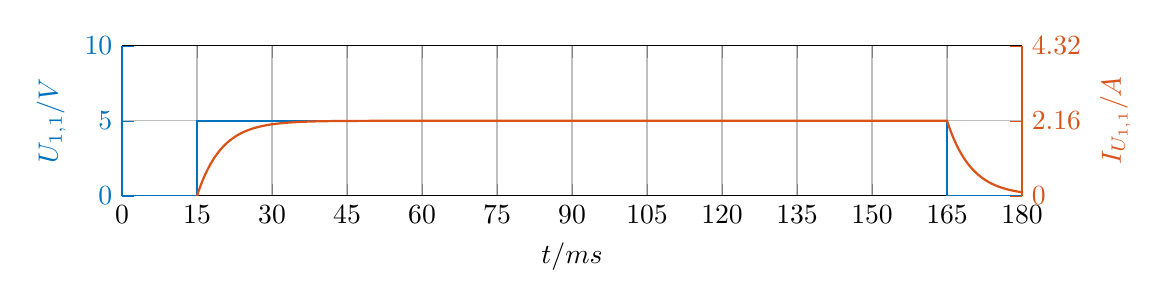
\begin{tikzpicture}
\pgfplotsset{
	width=4.5in,
	height=0.75in,
	every axis plot/.append style={thick}
}


\begin{axis}[%
scale only axis,
axis y line*=left,
ymin=0,
ymax=10,
xmin=0, xmax=180,
xtick={0,15,30,45,60,75,90,105,120,135,150,165,180},
xlabel={$ t/ms $},
ytick={ 0, 5, 10},
ylabel style={font=\color{mycolor1}},
ylabel={$ U_{1,1}/V $},
ytick style={mycolor1},
yticklabel style={mycolor1},
y axis line style={mycolor1},
xmajorgrids,
ymajorgrids
]
\addplot[const plot, color=mycolor1] table[row sep=crcr] {%
-1	0\\
-0.9	0\\
-0.8	0\\
-0.7	0\\
-0.6	0\\
-0.5	0\\
-0.4	0\\
-0.3	0\\
-0.2	0\\
-0.1	0\\
0	0\\
0.1	0\\
0.2	0\\
0.3	0\\
0.4	0\\
0.5	0\\
0.6	0\\
0.7	0\\
0.8	0\\
0.9	0\\
1	0\\
1.1	0\\
1.2	0\\
1.3	0\\
1.4	0\\
1.5	0\\
1.6	0\\
1.7	0\\
1.8	0\\
1.9	0\\
2	0\\
2.1	0\\
2.2	0\\
2.3	0\\
2.4	0\\
2.5	0\\
2.6	0\\
2.7	0\\
2.8	0\\
2.9	0\\
3	0\\
3.1	0\\
3.2	0\\
3.3	0\\
3.4	0\\
3.5	0\\
3.6	0\\
3.7	0\\
3.8	0\\
3.9	0\\
4	0\\
4.1	0\\
4.2	0\\
4.3	0\\
4.4	0\\
4.5	0\\
4.6	0\\
4.7	0\\
4.8	0\\
4.9	0\\
5	0\\
5.1	0\\
5.2	0\\
5.3	0\\
5.4	0\\
5.5	0\\
5.6	0\\
5.7	0\\
5.8	0\\
5.9	0\\
6	0\\
6.1	0\\
6.2	0\\
6.3	0\\
6.4	0\\
6.5	0\\
6.6	0\\
6.7	0\\
6.8	0\\
6.9	0\\
7	0\\
7.1	0\\
7.2	0\\
7.3	0\\
7.4	0\\
7.5	0\\
7.6	0\\
7.7	0\\
7.8	0\\
7.9	0\\
8	0\\
8.1	0\\
8.2	0\\
8.3	0\\
8.4	0\\
8.5	0\\
8.6	0\\
8.7	0\\
8.8	0\\
8.9	0\\
9	0\\
9.1	0\\
9.2	0\\
9.3	0\\
9.4	0\\
9.5	0\\
9.6	0\\
9.7	0\\
9.8	0\\
9.9	0\\
10	0\\
10.1	0\\
10.2	0\\
10.3	0\\
10.4	0\\
10.5	0\\
10.6	0\\
10.7	0\\
10.8	0\\
10.9	0\\
11	0\\
11.1	0\\
11.2	0\\
11.3	0\\
11.4	0\\
11.5	0\\
11.6	0\\
11.7	0\\
11.8	0\\
11.9	0\\
12	0\\
12.1	0\\
12.2	0\\
12.3	0\\
12.4	0\\
12.5	0\\
12.6	0\\
12.7	0\\
12.8	0\\
12.9	0\\
13	0\\
13.1	0\\
13.2	0\\
13.3	0\\
13.4	0\\
13.5	0\\
13.6	0\\
13.7	0\\
13.8	0\\
13.9	0\\
14	0\\
14.1	0\\
14.2	0\\
14.3	0\\
14.4	0\\
14.5	0\\
14.6	0\\
14.7	0\\
14.8	0\\
14.9	0\\
15	5\\
15.1	5\\
15.2	5\\
15.3	5\\
15.4	5\\
15.5	5\\
15.6	5\\
15.7	5\\
15.8	5\\
15.9	5\\
16	5\\
16.1	5\\
16.2	5\\
16.3	5\\
16.4	5\\
16.5	5\\
16.6	5\\
16.7	5\\
16.8	5\\
16.9	5\\
17	5\\
17.1	5\\
17.2	5\\
17.3	5\\
17.4	5\\
17.5	5\\
17.6	5\\
17.7	5\\
17.8	5\\
17.9	5\\
18	5\\
18.1	5\\
18.2	5\\
18.3	5\\
18.4	5\\
18.5	5\\
18.6	5\\
18.7	5\\
18.8	5\\
18.9	5\\
19	5\\
19.1	5\\
19.2	5\\
19.3	5\\
19.4	5\\
19.5	5\\
19.6	5\\
19.7	5\\
19.8	5\\
19.9	5\\
20	5\\
20.1	5\\
20.2	5\\
20.3	5\\
20.4	5\\
20.5	5\\
20.6	5\\
20.7	5\\
20.8	5\\
20.9	5\\
21	5\\
21.1	5\\
21.2	5\\
21.3	5\\
21.4	5\\
21.5	5\\
21.6	5\\
21.7	5\\
21.8	5\\
21.9	5\\
22	5\\
22.1	5\\
22.2	5\\
22.3	5\\
22.4	5\\
22.5	5\\
22.6	5\\
22.7	5\\
22.8	5\\
22.9	5\\
23	5\\
23.1	5\\
23.2	5\\
23.3	5\\
23.4	5\\
23.5	5\\
23.6	5\\
23.7	5\\
23.8	5\\
23.9	5\\
24	5\\
24.1	5\\
24.2	5\\
24.3	5\\
24.4	5\\
24.5	5\\
24.6	5\\
24.7	5\\
24.8	5\\
24.9	5\\
25	5\\
25.1	5\\
25.2	5\\
25.3	5\\
25.4	5\\
25.5	5\\
25.6	5\\
25.7	5\\
25.8	5\\
25.9	5\\
26	5\\
26.1	5\\
26.2	5\\
26.3	5\\
26.4	5\\
26.5	5\\
26.6	5\\
26.7	5\\
26.8	5\\
26.9	5\\
27	5\\
27.1	5\\
27.2	5\\
27.3	5\\
27.4	5\\
27.5	5\\
27.6	5\\
27.7	5\\
27.8	5\\
27.9	5\\
28	5\\
28.1	5\\
28.2	5\\
28.3	5\\
28.4	5\\
28.5	5\\
28.6	5\\
28.7	5\\
28.8	5\\
28.9	5\\
29	5\\
29.1	5\\
29.2	5\\
29.3	5\\
29.4	5\\
29.5	5\\
29.6	5\\
29.7	5\\
29.8	5\\
29.9	5\\
30	5\\
30.1	5\\
30.2	5\\
30.3	5\\
30.4	5\\
30.5	5\\
30.6	5\\
30.7	5\\
30.8	5\\
30.9	5\\
31	5\\
31.1	5\\
31.2	5\\
31.3	5\\
31.4	5\\
31.5	5\\
31.6	5\\
31.7	5\\
31.8	5\\
31.9	5\\
32	5\\
32.1	5\\
32.2	5\\
32.3	5\\
32.4	5\\
32.5	5\\
32.6	5\\
32.7	5\\
32.8	5\\
32.9	5\\
33	5\\
33.1	5\\
33.2	5\\
33.3	5\\
33.4	5\\
33.5	5\\
33.6	5\\
33.7	5\\
33.8	5\\
33.9	5\\
34	5\\
34.1	5\\
34.2	5\\
34.3	5\\
34.4	5\\
34.5	5\\
34.6	5\\
34.7	5\\
34.8	5\\
34.9	5\\
35	5\\
35.1	5\\
35.2	5\\
35.3	5\\
35.4	5\\
35.5	5\\
35.6	5\\
35.7	5\\
35.8	5\\
35.9	5\\
36	5\\
36.1	5\\
36.2	5\\
36.3	5\\
36.4	5\\
36.5	5\\
36.6	5\\
36.7	5\\
36.8	5\\
36.9	5\\
37	5\\
37.1	5\\
37.2	5\\
37.3	5\\
37.4	5\\
37.5	5\\
37.6	5\\
37.7	5\\
37.8	5\\
37.9	5\\
38	5\\
38.1	5\\
38.2	5\\
38.3	5\\
38.4	5\\
38.5	5\\
38.6	5\\
38.7	5\\
38.8	5\\
38.9	5\\
39	5\\
39.1	5\\
39.2	5\\
39.3	5\\
39.4	5\\
39.5	5\\
39.6	5\\
39.7	5\\
39.8	5\\
39.9	5\\
40	5\\
40.1	5\\
40.2	5\\
40.3	5\\
40.4	5\\
40.5	5\\
40.6	5\\
40.7	5\\
40.8	5\\
40.9	5\\
41	5\\
41.1	5\\
41.2	5\\
41.3	5\\
41.4	5\\
41.5	5\\
41.6	5\\
41.7	5\\
41.8	5\\
41.9	5\\
42	5\\
42.1	5\\
42.2	5\\
42.3	5\\
42.4	5\\
42.5	5\\
42.6	5\\
42.7	5\\
42.8	5\\
42.9	5\\
43	5\\
43.1	5\\
43.2	5\\
43.3	5\\
43.4	5\\
43.5	5\\
43.6	5\\
43.7	5\\
43.8	5\\
43.9	5\\
44	5\\
44.1	5\\
44.2	5\\
44.3	5\\
44.4	5\\
44.5	5\\
44.6	5\\
44.7	5\\
44.8	5\\
44.9	5\\
45	5\\
45.1	5\\
45.2	5\\
45.3	5\\
45.4	5\\
45.5	5\\
45.6	5\\
45.7	5\\
45.8	5\\
45.9	5\\
46	5\\
46.1	5\\
46.2	5\\
46.3	5\\
46.4	5\\
46.5	5\\
46.6	5\\
46.7	5\\
46.8	5\\
46.9	5\\
47	5\\
47.1	5\\
47.2	5\\
47.3	5\\
47.4	5\\
47.5	5\\
47.6	5\\
47.7	5\\
47.8	5\\
47.9	5\\
48	5\\
48.1	5\\
48.2	5\\
48.3	5\\
48.4	5\\
48.5	5\\
48.6	5\\
48.7	5\\
48.8	5\\
48.9	5\\
49	5\\
49.1	5\\
49.2	5\\
49.3	5\\
49.4	5\\
49.5	5\\
49.6	5\\
49.7	5\\
49.8	5\\
49.9	5\\
50	5\\
50.1	5\\
50.2	5\\
50.3	5\\
50.4	5\\
50.5	5\\
50.6	5\\
50.7	5\\
50.8	5\\
50.9	5\\
51	5\\
51.1	5\\
51.2	5\\
51.3	5\\
51.4	5\\
51.5	5\\
51.6	5\\
51.7	5\\
51.8	5\\
51.9	5\\
52	5\\
52.1	5\\
52.2	5\\
52.3	5\\
52.4	5\\
52.5	5\\
52.6	5\\
52.7	5\\
52.8	5\\
52.9	5\\
53	5\\
53.1	5\\
53.2	5\\
53.3	5\\
53.4	5\\
53.5	5\\
53.6	5\\
53.7	5\\
53.8	5\\
53.9	5\\
54	5\\
54.1	5\\
54.2	5\\
54.3	5\\
54.4	5\\
54.5	5\\
54.6	5\\
54.7	5\\
54.8	5\\
54.9	5\\
55	5\\
55.1	5\\
55.2	5\\
55.3	5\\
55.4	5\\
55.5	5\\
55.6	5\\
55.7	5\\
55.8	5\\
55.9	5\\
56	5\\
56.1	5\\
56.2	5\\
56.3	5\\
56.4	5\\
56.5	5\\
56.6	5\\
56.7	5\\
56.8	5\\
56.9	5\\
57	5\\
57.1	5\\
57.2	5\\
57.3	5\\
57.4	5\\
57.5	5\\
57.6	5\\
57.7	5\\
57.8	5\\
57.9	5\\
58	5\\
58.1	5\\
58.2	5\\
58.3	5\\
58.4	5\\
58.5	5\\
58.6	5\\
58.7	5\\
58.8	5\\
58.9	5\\
59	5\\
59.1	5\\
59.2	5\\
59.3	5\\
59.4	5\\
59.5	5\\
59.6	5\\
59.7	5\\
59.8	5\\
59.9	5\\
60	5\\
60.1	5\\
60.2	5\\
60.3	5\\
60.4	5\\
60.5	5\\
60.6	5\\
60.7	5\\
60.8	5\\
60.9	5\\
61	5\\
61.1	5\\
61.2	5\\
61.3	5\\
61.4	5\\
61.5	5\\
61.6	5\\
61.7	5\\
61.8	5\\
61.9	5\\
62	5\\
62.1	5\\
62.2	5\\
62.3	5\\
62.4	5\\
62.5	5\\
62.6	5\\
62.7	5\\
62.8	5\\
62.9	5\\
63	5\\
63.1	5\\
63.2	5\\
63.3	5\\
63.4	5\\
63.5	5\\
63.6	5\\
63.7	5\\
63.8	5\\
63.9	5\\
64	5\\
64.1	5\\
64.2	5\\
64.3	5\\
64.4	5\\
64.5	5\\
64.6	5\\
64.7	5\\
64.8	5\\
64.9	5\\
65	5\\
65.1	5\\
65.2	5\\
65.3	5\\
65.4	5\\
65.5	5\\
65.6	5\\
65.7	5\\
65.8	5\\
65.9	5\\
66	5\\
66.1	5\\
66.2	5\\
66.3	5\\
66.4	5\\
66.5	5\\
66.6	5\\
66.7	5\\
66.8	5\\
66.9	5\\
67	5\\
67.1	5\\
67.2	5\\
67.3	5\\
67.4	5\\
67.5	5\\
67.6	5\\
67.7	5\\
67.8	5\\
67.9	5\\
68	5\\
68.1	5\\
68.2	5\\
68.3	5\\
68.4	5\\
68.5	5\\
68.6	5\\
68.7	5\\
68.8	5\\
68.9	5\\
69	5\\
69.1	5\\
69.2	5\\
69.3	5\\
69.4	5\\
69.5	5\\
69.6	5\\
69.7	5\\
69.8	5\\
69.9	5\\
70	5\\
70.1	5\\
70.2	5\\
70.3	5\\
70.4	5\\
70.5	5\\
70.6	5\\
70.7	5\\
70.8	5\\
70.9	5\\
71	5\\
71.1	5\\
71.2	5\\
71.3	5\\
71.4	5\\
71.5	5\\
71.6	5\\
71.7	5\\
71.8	5\\
71.9	5\\
72	5\\
72.1	5\\
72.2	5\\
72.3	5\\
72.4	5\\
72.5	5\\
72.6	5\\
72.7	5\\
72.8	5\\
72.9	5\\
73	5\\
73.1	5\\
73.2	5\\
73.3	5\\
73.4	5\\
73.5	5\\
73.6	5\\
73.7	5\\
73.8	5\\
73.9	5\\
74	5\\
74.1	5\\
74.2	5\\
74.3	5\\
74.4	5\\
74.5	5\\
74.6	5\\
74.7	5\\
74.8	5\\
74.9	5\\
75	5\\
75.1	5\\
75.2	5\\
75.3	5\\
75.4	5\\
75.5	5\\
75.6	5\\
75.7	5\\
75.8	5\\
75.9	5\\
76	5\\
76.1	5\\
76.2	5\\
76.3	5\\
76.4	5\\
76.5	5\\
76.6	5\\
76.7	5\\
76.8	5\\
76.9	5\\
77	5\\
77.1	5\\
77.2	5\\
77.3	5\\
77.4	5\\
77.5	5\\
77.6	5\\
77.7	5\\
77.8	5\\
77.9	5\\
78	5\\
78.1	5\\
78.2	5\\
78.3	5\\
78.4	5\\
78.5	5\\
78.6	5\\
78.7	5\\
78.8	5\\
78.9	5\\
79	5\\
79.1	5\\
79.2	5\\
79.3	5\\
79.4	5\\
79.5	5\\
79.6	5\\
79.7	5\\
79.8	5\\
79.9	5\\
80	5\\
80.1	5\\
80.2	5\\
80.3	5\\
80.4	5\\
80.5	5\\
80.6	5\\
80.7	5\\
80.8	5\\
80.9	5\\
81	5\\
81.1	5\\
81.2	5\\
81.3	5\\
81.4	5\\
81.5	5\\
81.6	5\\
81.7	5\\
81.8	5\\
81.9	5\\
82	5\\
82.1	5\\
82.2	5\\
82.3	5\\
82.4	5\\
82.5	5\\
82.6	5\\
82.7	5\\
82.8	5\\
82.9	5\\
83	5\\
83.1	5\\
83.2	5\\
83.3	5\\
83.4	5\\
83.5	5\\
83.6	5\\
83.7	5\\
83.8	5\\
83.9	5\\
84	5\\
84.1	5\\
84.2	5\\
84.3	5\\
84.4	5\\
84.5	5\\
84.6	5\\
84.7	5\\
84.8	5\\
84.9	5\\
85	5\\
85.1	5\\
85.2	5\\
85.3	5\\
85.4	5\\
85.5	5\\
85.6	5\\
85.7	5\\
85.8	5\\
85.9	5\\
86	5\\
86.1	5\\
86.2	5\\
86.3	5\\
86.4	5\\
86.5	5\\
86.6	5\\
86.7	5\\
86.8	5\\
86.9	5\\
87	5\\
87.1	5\\
87.2	5\\
87.3	5\\
87.4	5\\
87.5	5\\
87.6	5\\
87.7	5\\
87.8	5\\
87.9	5\\
88	5\\
88.1	5\\
88.2	5\\
88.3	5\\
88.4	5\\
88.5	5\\
88.6	5\\
88.7	5\\
88.8	5\\
88.9	5\\
89	5\\
89.1	5\\
89.2	5\\
89.3	5\\
89.4	5\\
89.5	5\\
89.6	5\\
89.7	5\\
89.8	5\\
89.9	5\\
90	5\\
90.1	5\\
90.2	5\\
90.3	5\\
90.4	5\\
90.5	5\\
90.6	5\\
90.7	5\\
90.8	5\\
90.9	5\\
91	5\\
91.1	5\\
91.2	5\\
91.3	5\\
91.4	5\\
91.5	5\\
91.6	5\\
91.7	5\\
91.8	5\\
91.9	5\\
92	5\\
92.1	5\\
92.2	5\\
92.3	5\\
92.4	5\\
92.5	5\\
92.6	5\\
92.7	5\\
92.8	5\\
92.9	5\\
93	5\\
93.1	5\\
93.2	5\\
93.3	5\\
93.4	5\\
93.5	5\\
93.6	5\\
93.7	5\\
93.8	5\\
93.9	5\\
94	5\\
94.1	5\\
94.2	5\\
94.3	5\\
94.4	5\\
94.5	5\\
94.6	5\\
94.7	5\\
94.8	5\\
94.9	5\\
95	5\\
95.1	5\\
95.2	5\\
95.3	5\\
95.4	5\\
95.5	5\\
95.6	5\\
95.7	5\\
95.8	5\\
95.9	5\\
96	5\\
96.1	5\\
96.2	5\\
96.3	5\\
96.4	5\\
96.5	5\\
96.6	5\\
96.7	5\\
96.8	5\\
96.9	5\\
97	5\\
97.1	5\\
97.2	5\\
97.3	5\\
97.4	5\\
97.5	5\\
97.6	5\\
97.7	5\\
97.8	5\\
97.9	5\\
98	5\\
98.1	5\\
98.2	5\\
98.3	5\\
98.4	5\\
98.5	5\\
98.6	5\\
98.7	5\\
98.8	5\\
98.9	5\\
99	5\\
99.1	5\\
99.2	5\\
99.3	5\\
99.4	5\\
99.5	5\\
99.6	5\\
99.7	5\\
99.8	5\\
99.9	5\\
100	5\\
100.1	5\\
100.2	5\\
100.3	5\\
100.4	5\\
100.5	5\\
100.6	5\\
100.7	5\\
100.8	5\\
100.9	5\\
101	5\\
101.1	5\\
101.2	5\\
101.3	5\\
101.4	5\\
101.5	5\\
101.6	5\\
101.7	5\\
101.8	5\\
101.9	5\\
102	5\\
102.1	5\\
102.2	5\\
102.3	5\\
102.4	5\\
102.5	5\\
102.6	5\\
102.7	5\\
102.8	5\\
102.9	5\\
103	5\\
103.1	5\\
103.2	5\\
103.3	5\\
103.4	5\\
103.5	5\\
103.6	5\\
103.7	5\\
103.8	5\\
103.9	5\\
104	5\\
104.1	5\\
104.2	5\\
104.3	5\\
104.4	5\\
104.5	5\\
104.6	5\\
104.7	5\\
104.8	5\\
104.9	5\\
105	5\\
105.1	5\\
105.2	5\\
105.3	5\\
105.4	5\\
105.5	5\\
105.6	5\\
105.7	5\\
105.8	5\\
105.9	5\\
106	5\\
106.1	5\\
106.2	5\\
106.3	5\\
106.4	5\\
106.5	5\\
106.6	5\\
106.7	5\\
106.8	5\\
106.9	5\\
107	5\\
107.1	5\\
107.2	5\\
107.3	5\\
107.4	5\\
107.5	5\\
107.6	5\\
107.7	5\\
107.8	5\\
107.9	5\\
108	5\\
108.1	5\\
108.2	5\\
108.3	5\\
108.4	5\\
108.5	5\\
108.6	5\\
108.7	5\\
108.8	5\\
108.9	5\\
109	5\\
109.1	5\\
109.2	5\\
109.3	5\\
109.4	5\\
109.5	5\\
109.6	5\\
109.7	5\\
109.8	5\\
109.9	5\\
110	5\\
110.1	5\\
110.2	5\\
110.3	5\\
110.4	5\\
110.5	5\\
110.6	5\\
110.7	5\\
110.8	5\\
110.9	5\\
111	5\\
111.1	5\\
111.2	5\\
111.3	5\\
111.4	5\\
111.5	5\\
111.6	5\\
111.7	5\\
111.8	5\\
111.9	5\\
112	5\\
112.1	5\\
112.2	5\\
112.3	5\\
112.4	5\\
112.5	5\\
112.6	5\\
112.7	5\\
112.8	5\\
112.9	5\\
113	5\\
113.1	5\\
113.2	5\\
113.3	5\\
113.4	5\\
113.5	5\\
113.6	5\\
113.7	5\\
113.8	5\\
113.9	5\\
114	5\\
114.1	5\\
114.2	5\\
114.3	5\\
114.4	5\\
114.5	5\\
114.6	5\\
114.7	5\\
114.8	5\\
114.9	5\\
115	5\\
115.1	5\\
115.2	5\\
115.3	5\\
115.4	5\\
115.5	5\\
115.6	5\\
115.7	5\\
115.8	5\\
115.9	5\\
116	5\\
116.1	5\\
116.2	5\\
116.3	5\\
116.4	5\\
116.5	5\\
116.6	5\\
116.7	5\\
116.8	5\\
116.9	5\\
117	5\\
117.1	5\\
117.2	5\\
117.3	5\\
117.4	5\\
117.5	5\\
117.6	5\\
117.7	5\\
117.8	5\\
117.9	5\\
118	5\\
118.1	5\\
118.2	5\\
118.3	5\\
118.4	5\\
118.5	5\\
118.6	5\\
118.7	5\\
118.8	5\\
118.9	5\\
119	5\\
119.1	5\\
119.2	5\\
119.3	5\\
119.4	5\\
119.5	5\\
119.6	5\\
119.7	5\\
119.8	5\\
119.9	5\\
120	5\\
120.1	5\\
120.2	5\\
120.3	5\\
120.4	5\\
120.5	5\\
120.6	5\\
120.7	5\\
120.8	5\\
120.9	5\\
121	5\\
121.1	5\\
121.2	5\\
121.3	5\\
121.4	5\\
121.5	5\\
121.6	5\\
121.7	5\\
121.8	5\\
121.9	5\\
122	5\\
122.1	5\\
122.2	5\\
122.3	5\\
122.4	5\\
122.5	5\\
122.6	5\\
122.7	5\\
122.8	5\\
122.9	5\\
123	5\\
123.1	5\\
123.2	5\\
123.3	5\\
123.4	5\\
123.5	5\\
123.6	5\\
123.7	5\\
123.8	5\\
123.9	5\\
124	5\\
124.1	5\\
124.2	5\\
124.3	5\\
124.4	5\\
124.5	5\\
124.6	5\\
124.7	5\\
124.8	5\\
124.9	5\\
125	5\\
125.1	5\\
125.2	5\\
125.3	5\\
125.4	5\\
125.5	5\\
125.6	5\\
125.7	5\\
125.8	5\\
125.9	5\\
126	5\\
126.1	5\\
126.2	5\\
126.3	5\\
126.4	5\\
126.5	5\\
126.6	5\\
126.7	5\\
126.8	5\\
126.9	5\\
127	5\\
127.1	5\\
127.2	5\\
127.3	5\\
127.4	5\\
127.5	5\\
127.6	5\\
127.7	5\\
127.8	5\\
127.9	5\\
128	5\\
128.1	5\\
128.2	5\\
128.3	5\\
128.4	5\\
128.5	5\\
128.6	5\\
128.7	5\\
128.8	5\\
128.9	5\\
129	5\\
129.1	5\\
129.2	5\\
129.3	5\\
129.4	5\\
129.5	5\\
129.6	5\\
129.7	5\\
129.8	5\\
129.9	5\\
130	5\\
130.1	5\\
130.2	5\\
130.3	5\\
130.4	5\\
130.5	5\\
130.6	5\\
130.7	5\\
130.8	5\\
130.9	5\\
131	5\\
131.1	5\\
131.2	5\\
131.3	5\\
131.4	5\\
131.5	5\\
131.6	5\\
131.7	5\\
131.8	5\\
131.9	5\\
132	5\\
132.1	5\\
132.2	5\\
132.3	5\\
132.4	5\\
132.5	5\\
132.6	5\\
132.7	5\\
132.8	5\\
132.9	5\\
133	5\\
133.1	5\\
133.2	5\\
133.3	5\\
133.4	5\\
133.5	5\\
133.6	5\\
133.7	5\\
133.8	5\\
133.9	5\\
134	5\\
134.1	5\\
134.2	5\\
134.3	5\\
134.4	5\\
134.5	5\\
134.6	5\\
134.7	5\\
134.8	5\\
134.9	5\\
135	5\\
135.1	5\\
135.2	5\\
135.3	5\\
135.4	5\\
135.5	5\\
135.6	5\\
135.7	5\\
135.8	5\\
135.9	5\\
136	5\\
136.1	5\\
136.2	5\\
136.3	5\\
136.4	5\\
136.5	5\\
136.6	5\\
136.7	5\\
136.8	5\\
136.9	5\\
137	5\\
137.1	5\\
137.2	5\\
137.3	5\\
137.4	5\\
137.5	5\\
137.6	5\\
137.7	5\\
137.8	5\\
137.9	5\\
138	5\\
138.1	5\\
138.2	5\\
138.3	5\\
138.4	5\\
138.5	5\\
138.6	5\\
138.7	5\\
138.8	5\\
138.9	5\\
139	5\\
139.1	5\\
139.2	5\\
139.3	5\\
139.4	5\\
139.5	5\\
139.6	5\\
139.7	5\\
139.8	5\\
139.9	5\\
140	5\\
140.1	5\\
140.2	5\\
140.3	5\\
140.4	5\\
140.5	5\\
140.6	5\\
140.7	5\\
140.8	5\\
140.9	5\\
141	5\\
141.1	5\\
141.2	5\\
141.3	5\\
141.4	5\\
141.5	5\\
141.6	5\\
141.7	5\\
141.8	5\\
141.9	5\\
142	5\\
142.1	5\\
142.2	5\\
142.3	5\\
142.4	5\\
142.5	5\\
142.6	5\\
142.7	5\\
142.8	5\\
142.9	5\\
143	5\\
143.1	5\\
143.2	5\\
143.3	5\\
143.4	5\\
143.5	5\\
143.6	5\\
143.7	5\\
143.8	5\\
143.9	5\\
144	5\\
144.1	5\\
144.2	5\\
144.3	5\\
144.4	5\\
144.5	5\\
144.6	5\\
144.7	5\\
144.8	5\\
144.9	5\\
145	5\\
145.1	5\\
145.2	5\\
145.3	5\\
145.4	5\\
145.5	5\\
145.6	5\\
145.7	5\\
145.8	5\\
145.9	5\\
146	5\\
146.1	5\\
146.2	5\\
146.3	5\\
146.4	5\\
146.5	5\\
146.6	5\\
146.7	5\\
146.8	5\\
146.9	5\\
147	5\\
147.1	5\\
147.2	5\\
147.3	5\\
147.4	5\\
147.5	5\\
147.6	5\\
147.7	5\\
147.8	5\\
147.9	5\\
148	5\\
148.1	5\\
148.2	5\\
148.3	5\\
148.4	5\\
148.5	5\\
148.6	5\\
148.7	5\\
148.8	5\\
148.9	5\\
149	5\\
149.1	5\\
149.2	5\\
149.3	5\\
149.4	5\\
149.5	5\\
149.6	5\\
149.7	5\\
149.8	5\\
149.9	5\\
150	5\\
150.1	5\\
150.2	5\\
150.3	5\\
150.4	5\\
150.5	5\\
150.6	5\\
150.7	5\\
150.8	5\\
150.9	5\\
151	5\\
151.1	5\\
151.2	5\\
151.3	5\\
151.4	5\\
151.5	5\\
151.6	5\\
151.7	5\\
151.8	5\\
151.9	5\\
152	5\\
152.1	5\\
152.2	5\\
152.3	5\\
152.4	5\\
152.5	5\\
152.6	5\\
152.7	5\\
152.8	5\\
152.9	5\\
153	5\\
153.1	5\\
153.2	5\\
153.3	5\\
153.4	5\\
153.5	5\\
153.6	5\\
153.7	5\\
153.8	5\\
153.9	5\\
154	5\\
154.1	5\\
154.2	5\\
154.3	5\\
154.4	5\\
154.5	5\\
154.6	5\\
154.7	5\\
154.8	5\\
154.9	5\\
155	5\\
155.1	5\\
155.2	5\\
155.3	5\\
155.4	5\\
155.5	5\\
155.6	5\\
155.7	5\\
155.8	5\\
155.9	5\\
156	5\\
156.1	5\\
156.2	5\\
156.3	5\\
156.4	5\\
156.5	5\\
156.6	5\\
156.7	5\\
156.8	5\\
156.9	5\\
157	5\\
157.1	5\\
157.2	5\\
157.3	5\\
157.4	5\\
157.5	5\\
157.6	5\\
157.7	5\\
157.8	5\\
157.9	5\\
158	5\\
158.1	5\\
158.2	5\\
158.3	5\\
158.4	5\\
158.5	5\\
158.6	5\\
158.7	5\\
158.8	5\\
158.9	5\\
159	5\\
159.1	5\\
159.2	5\\
159.3	5\\
159.4	5\\
159.5	5\\
159.6	5\\
159.7	5\\
159.8	5\\
159.9	5\\
160	5\\
160.1	5\\
160.2	5\\
160.3	5\\
160.4	5\\
160.5	5\\
160.6	5\\
160.7	5\\
160.8	5\\
160.9	5\\
161	5\\
161.1	5\\
161.2	5\\
161.3	5\\
161.4	5\\
161.5	5\\
161.6	5\\
161.7	5\\
161.8	5\\
161.9	5\\
162	5\\
162.1	5\\
162.2	5\\
162.3	5\\
162.4	5\\
162.5	5\\
162.6	5\\
162.7	5\\
162.8	5\\
162.9	5\\
163	5\\
163.1	5\\
163.2	5\\
163.3	5\\
163.4	5\\
163.5	5\\
163.6	5\\
163.7	5\\
163.8	5\\
163.9	5\\
164	5\\
164.1	5\\
164.2	5\\
164.3	5\\
164.4	5\\
164.5	5\\
164.6	5\\
164.7	5\\
164.8	5\\
164.9	5\\
165	 0\\
165.1	0\\
165.2	0\\
165.3	0\\
165.4	0\\
165.5	0\\
165.6	0\\
165.7	0\\
165.8	0\\
165.9	0\\
166	0\\
166.1	0\\
166.2	0\\
166.3	0\\
166.4	0\\
166.5	0\\
166.6	0\\
166.7	0\\
166.8	0\\
166.9	0\\
167	0\\
167.1	0\\
167.2	0\\
167.3	0\\
167.4	0\\
167.5	0\\
167.6	0\\
167.7	0\\
167.8	0\\
167.9	0\\
168	0\\
168.1	0\\
168.2	0\\
168.3	0\\
168.4	0\\
168.5	0\\
168.6	0\\
168.7	0\\
168.8	0\\
168.9	0\\
169	0\\
169.1	0\\
169.2	0\\
169.3	0\\
169.4	0\\
169.5	0\\
169.6	0\\
169.7	0\\
169.8	0\\
169.9	0\\
170	0\\
170.1	0\\
170.2	0\\
170.3	0\\
170.4	0\\
170.5	0\\
170.6	0\\
170.7	0\\
170.8	0\\
170.9	0\\
171	0\\
171.1	0\\
171.2	0\\
171.3	0\\
171.4	0\\
171.5	0\\
171.6	0\\
171.7	0\\
171.8	0\\
171.9	0\\
172	0\\
172.1	0\\
172.2	0\\
172.3	0\\
172.4	0\\
172.5	0\\
172.6	0\\
172.7	0\\
172.8	0\\
172.9	0\\
173	0\\
173.1	0\\
173.2	0\\
173.3	0\\
173.4	0\\
173.5	0\\
173.6	0\\
173.7	0\\
173.8	0\\
173.9	0\\
174	0\\
174.1	0\\
174.2	0\\
174.3	0\\
174.4	0\\
174.5	0\\
174.6	0\\
174.7	0\\
174.8	0\\
174.9	0\\
175	0\\
175.1	0\\
175.2	0\\
175.3	0\\
175.4	0\\
175.5	0\\
175.6	0\\
175.7	0\\
175.8	0\\
175.9	0\\
176	0\\
176.1	0\\
176.2	0\\
176.3	0\\
176.4	0\\
176.5	0\\
176.6	0\\
176.7	0\\
176.8	0\\
176.9	0\\
177	0\\
177.1	0\\
177.2	0\\
177.3	0\\
177.4	0\\
177.5	0\\
177.6	0\\
177.7	0\\
177.8	0\\
177.9	0\\
178	0\\
178.1	0\\
178.2	0\\
178.3	0\\
178.4	0\\
178.5	0\\
178.6	0\\
178.7	0\\
178.8	0\\
178.9	0\\
179	0\\
179.1	0\\
179.2	0\\
179.3	0\\
179.4	0\\
179.5	0\\
179.6	0\\
179.7	0\\
179.8	0\\
179.9	0\\
180	0\\
};
\end{axis}

\begin{axis}[
scale only axis,
axis y line*=right,
axis x line=none,
xmin=0,
xmax=180,
ymin=0,
ymax=4.32,
ytick={   0, 2.16, 4.32},
ytick style={mycolor2},
ylabel style={font=\color{mycolor2}},
yticklabel style={mycolor2},
y axis line style={mycolor2},
ylabel={$ I_{U_{1,1}}/A $}
]
\addplot [color=mycolor2]
  table[row sep=crcr]{%
-1	-56.1914171888181\\
-0.9	-55.0585644770092\\
-0.8	-53.9485507561148\\
-0.7	-52.8609155783641\\
-0.6	-51.7952077788895\\
-0.5	-50.7509852885784\\
-0.4	-49.7278149506966\\
-0.3	-48.72527234121\\
-0.2	-47.7429415927277\\
-0.1	-46.7804152219955\\
0	-45.8372939608658\\
0.1	-44.9131865906768\\
0.2	-44.00770977997\\
0.3	-43.120487925479\\
0.4	-42.251152996325\\
0.5	-41.3993443813527\\
0.6	-40.564708739544\\
0.7	-39.7468998534483\\
0.8	-38.9455784855662\\
0.9	-38.1604122376303\\
1	-37.391075412722\\
1.1	-36.6372488801678\\
1.2	-35.8986199431604\\
1.3	-35.1748822090479\\
1.4	-34.4657354622381\\
1.5	-33.7708855396657\\
1.6	-33.0900442087691\\
1.7	-32.4229290479285\\
1.8	-31.7692633293133\\
1.9	-31.1287759040924\\
2	-30.5012010899576\\
2.1	-29.8862785609158\\
2.2	-29.2837532393024\\
2.3	-28.6933751899712\\
2.4	-28.1148995166191\\
2.5	-27.5480862601993\\
2.6	-26.9927002993835\\
2.7	-26.4485112530306\\
2.8	-25.9152933846216\\
2.9	-25.3928255086212\\
3	-24.8808908987275\\
3.1	-24.3792771979708\\
3.2	-23.8877763306256\\
3.3	-23.4061844158978\\
3.4	-22.9343016833525\\
3.5	-22.471932390047\\
3.6	-22.0188847393336\\
3.7	-21.5749708013002\\
3.8	-21.1400064348148\\
3.9	-20.713811211141\\
4	-20.2962083390941\\
4.1	-19.8870245917057\\
4.2	-19.4860902343675\\
4.3	-19.0932389544224\\
4.4	-18.7083077921765\\
4.5	-18.3311370733013\\
4.6	-17.9615703425985\\
4.7	-17.5994542991005\\
4.8	-17.2446387324794\\
4.9	-16.8969764607376\\
5	-16.5563232691551\\
5.1	-16.222537850467\\
5.2	-15.8954817462479\\
5.3	-15.5750192894774\\
5.4	-15.2610175482636\\
5.5	-14.9533462707014\\
5.6	-14.6518778308423\\
5.7	-14.3564871757537\\
5.8	-14.067051773645\\
5.9	-13.7834515630402\\
6	-13.5055689029748\\
6.1	-13.2332885241965\\
6.2	-12.9664974813508\\
6.3	-12.7050851061289\\
6.4	-12.4489429613619\\
6.5	-12.1979647960392\\
6.6	-11.9520465012343\\
6.7	-11.7110860669194\\
6.8	-11.4749835396498\\
6.9	-11.2436409811026\\
7	-11.0169624274501\\
7.1	-10.7948538495529\\
7.2	-10.5772231139558\\
7.3	-10.3639799446692\\
7.4	-10.1550358857215\\
7.5	-9.95030426446699\\
7.6	-9.74970015563223\\
7.7	-9.5531403460884\\
7.8	-9.36054330033332\\
7.9	-9.1718291266695\\
8	-8.986919544064\\
8.1	-8.80573784967657\\
8.2	-8.62820888704222\\
8.3	-8.45425901489547\\
8.4	-8.28381607662295\\
8.5	-8.11680937033194\\
8.6	-7.95316961952233\\
8.7	-7.79282894434988\\
8.8	-7.63572083346873\\
8.9	-7.48178011644172\\
9	-7.33094293670681\\
9.1	-7.18314672508861\\
9.2	-7.03833017384389\\
9.3	-6.89643321123032\\
9.4	-6.75739697658796\\
9.5	-6.62116379592313\\
9.6	-6.48767715798449\\
9.7	-6.35688169082148\\
9.8	-6.22872313881527\\
9.9	-6.10314834017293\\
10	-5.98010520487516\\
10.1	-5.85954269306875\\
10.2	-5.74141079389459\\
10.3	-5.62566050474248\\
10.4	-5.5122438109243\\
10.5	-5.40111366575686\\
10.6	-5.29222397104636\\
10.7	-5.18552955796626\\
10.8	-5.08098616832069\\
10.9	-4.97855043618558\\
11	-4.87817986991995\\
11.1	-4.77983283453978\\
11.2	-4.68346853444736\\
11.3	-4.58904699650871\\
11.4	-4.49652905347224\\
11.5	-4.40587632772168\\
11.6	-4.31705121535652\\
11.7	-4.23001687059349\\
11.8	-4.14473719048244\\
11.9	-4.06117679993034\\
12	-3.97930103702732\\
12.1	-3.89907593866839\\
12.2	-3.82046822646518\\
12.3	-3.74344529294158\\
12.4	-3.66797518800782\\
12.5	-3.59402660570708\\
12.6	-3.52156887122946\\
12.7	-3.45057192818763\\
12.8	-3.38100632614908\\
12.9	-3.31284320841972\\
13	-3.24605430007372\\
13.1	-3.18061189622473\\
13.2	-3.11648885053357\\
13.3	-3.05365856394753\\
13.4	-2.99209497366679\\
13.5	-2.93177254233322\\
13.6	-2.87266624743718\\
13.7	-2.81475157093781\\
13.8	-2.75800448909273\\
13.9	-2.70240146249258\\
14	-2.64791942629666\\
14.1	-2.5945357806653\\
14.2	-2.54222838138517\\
14.3	-2.49097553068357\\
14.4	-2.44075596822794\\
14.5	-2.39154886230677\\
14.6	-2.34333380118838\\
14.7	-2.29609078465385\\
14.8	-2.2498002157007\\
14.9	-2.20444289241375\\
15	-1.08\\
15.1	0.0435468970160487\\
15.2	0.0862158624396299\\
15.3	0.128024595898823\\
15.4	0.168990440186572\\
15.5	0.209130388454702\\
15.6	0.248461091262897\\
15.7	0.286998863485555\\
15.8	0.324759691079415\\
15.9	0.361759237714723\\
16	0.39801285127273\\
16.1	0.433535570212188\\
16.2	0.468342129807483\\
16.3	0.50244696826103\\
16.4	0.535864232692408\\
16.5	0.56860778500677\\
16.6	0.600691207644943\\
16.7	0.632127809217582\\
16.8	0.662930630025771\\
16.9	0.693112447470284\\
17	0.722685781351827\\
17.1	0.751662899064408\\
17.2	0.780055820684001\\
17.3	0.807876323954635\\
17.4	0.835135949173945\\
17.5	0.861846003980234\\
17.6	0.888017568043033\\
17.7	0.913661497659075\\
17.8	0.938788430255638\\
17.9	0.963408788803076\\
18	0.987532786138399\\
18.1	1.0111704292017\\
18.2	1.03433152318714\\
18.3	1.05702567561027\\
18.4	1.0792623002934\\
18.5	1.10105062127047\\
18.6	1.12239967661341\\
18.7	1.14331832218116\\
18.8	1.16381523529323\\
18.9	1.18389891832918\\
19	1.20357770225546\\
19.1	1.22285975008126\\
19.2	1.2417530602446\\
19.3	1.26026546993017\\
19.4	1.27840465832032\\
19.5	1.29617814978048\\
19.6	1.31359331698036\\
19.7	1.33065738395219\\
19.8	1.3473774290874\\
19.9	1.36376038807279\\
20	1.37981305676755\\
20.1	1.39554209402228\\
20.2	1.41095402444113\\
20.3	1.42605524108833\\
20.4	1.44085200814008\\
20.5	1.45535046348306\\
20.6	1.46955662126042\\
20.7	1.48347637436662\\
20.8	1.49711549689179\\
20.9	1.51047964651697\\
21	1.52357436686093\\
21.1	1.53640508977977\\
21.2	1.54897713762009\\
21.3	1.5612957254268\\
21.4	1.57336596310639\\
21.5	1.58519285754654\\
21.6	1.59678131469307\\
21.7	1.608136141585\\
21.8	1.61926204834856\\
21.9	1.63016365015098\\
22	1.64084546911498\\
22.1	1.65131193619454\\
22.2	1.66156739301298\\
22.3	1.67161609366386\\
22.4	1.68146220647568\\
22.5	1.6911098157409\\
22.6	1.70056292341024\\
22.7	1.70982545075265\\
22.8	1.71890123998197\\
22.9	1.72779405585068\\
23	1.7365075872116\\
23.1	1.74504544854807\\
23.2	1.75341118147326\\
23.3	1.76160825619931\\
23.4	1.76964007297678\\
23.5	1.77750996350514\\
23.6	1.78522119231482\\
23.7	1.79277695812133\\
23.8	1.80018039515217\\
23.9	1.80743457444692\\
24	1.81454250513117\\
24.1	1.82150713566473\\
24.2	1.82833135506467\\
24.3	1.83501799410377\\
24.4	1.84156982648471\\
24.5	1.84798956999067\\
24.6	1.85427988761268\\
24.7	1.86044338865428\\
24.8	1.86648262981389\\
24.9	1.87240011624533\\
25	1.87819830259704\\
25.1	1.88387959403026\\
25.2	1.88944634721674\\
25.3	1.89490087131631\\
25.4	1.90024542893475\\
25.5	1.90548223706235\\
25.6	1.91061346799356\\
25.7	1.91564125022804\\
25.8	1.92056766935363\\
25.9	1.92539476891149\\
26	1.93012455124373\\
26.1	1.93475897832406\\
26.2	1.93929997257161\\
26.3	1.9437494176484\\
26.4	1.94810915924068\\
26.5	1.95238100582456\\
26.6	1.9565667294162\\
26.7	1.96066806630682\\
26.8	1.964686717783\\
26.9	1.96862435083234\\
27	1.97248259883497\\
27.1	1.97626306224111\\
27.2	1.97996730923492\\
27.3	1.98359687638504\\
27.4	1.98715326928197\\
27.5	1.99063796316259\\
27.6	1.99405240352212\\
27.7	1.99739800671373\\
27.8	2.00067616053607\\
27.9	2.00388822480891\\
28	2.00703553193726\\
28.1	2.01011938746404\\
28.2	2.01314107061164\\
28.3	2.01610183481254\\
28.4	2.01900290822931\\
28.5	2.02184549426399\\
28.6	2.02463077205732\\
28.7	2.02735989697785\\
28.8	2.03003400110123\\
28.9	2.03265419367977\\
29	2.03522156160257\\
29.1	2.03773716984642\\
29.2	2.04020206191753\\
29.3	2.04261726028438\\
29.4	2.04498376680191\\
29.5	2.04730256312703\\
29.6	2.04957461112586\\
29.7	2.05180085327274\\
29.8	2.05398221304114\\
29.9	2.05611959528678\\
30	2.0582138866229\\
30.1	2.06026595578813\\
30.2	2.06227665400678\\
30.3	2.06424681534198\\
30.4	2.06617725704164\\
30.5	2.06806877987746\\
30.6	2.06992216847711\\
30.7	2.07173819164968\\
30.8	2.07351760270463\\
30.9	2.07526113976422\\
31	2.07696952606975\\
31.1	2.07864347028152\\
31.2	2.08028366677284\\
31.3	2.08189079591799\\
31.4	2.08346552437455\\
31.5	2.08500850535985\\
31.6	2.08652037892197\\
31.7	2.08800177220524\\
31.8	2.08945329971038\\
31.9	2.09087556354942\\
32	2.09226915369545\\
32.1	2.09363464822731\\
32.2	2.09497261356948\\
32.3	2.09628360472694\\
32.4	2.09756816551545\\
32.5	2.09882682878713\\
32.6	2.10006011665146\\
32.7	2.10126854069189\\
32.8	2.10245260217805\\
32.9	2.10361279227364\\
33	2.10474959224026\\
33.1	2.10586347363693\\
33.2	2.10695489851579\\
33.3	2.10802431961372\\
33.4	2.10907218054017\\
33.5	2.11009891596113\\
33.6	2.11110495177947\\
33.7	2.11209070531163\\
33.8	2.11305658546066\\
33.9	2.1140029928859\\
34	2.11493032016916\\
34.1	2.11583895197756\\
34.2	2.11672926522309\\
34.3	2.11760162921899\\
34.4	2.1184564058329\\
34.5	2.11929394963701\\
34.6	2.12011460805511\\
34.7	2.12091872150671\\
34.8	2.12170662354829\\
34.9	2.12247864101159\\
35	2.12323509413926\\
35.1	2.12397629671765\\
35.2	2.12470255620699\\
35.3	2.12541417386893\\
35.4	2.1261114448915\\
35.5	2.12679465851156\\
35.6	2.12746409813479\\
35.7	2.12812004145324\\
35.8	2.12876276056051\\
35.9	2.12939252206465\\
36	2.13000958719871\\
36.1	2.13061421192914\\
36.2	2.13120664706194\\
36.3	2.13178713834673\\
36.4	2.13235592657865\\
36.5	2.13291324769827\\
36.6	2.13345933288947\\
36.7	2.1339944086753\\
36.8	2.13451869701199\\
36.9	2.135032415381\\
37	2.13553577687921\\
37.1	2.13602899030737\\
37.2	2.13651226025666\\
37.3	2.13698578719357\\
37.4	2.13744976754311\\
37.5	2.13790439377018\\
37.6	2.13834985445953\\
37.7	2.1387863343939\\
37.8	2.1392140146307\\
37.9	2.13963307257711\\
38	2.14004368206369\\
38.1	2.14044601341647\\
38.2	2.14084023352758\\
38.3	2.14122650592454\\
38.4	2.14160499083803\\
38.5	2.14197584526839\\
38.6	2.14233922305075\\
38.7	2.14269527491882\\
38.8	2.14304414856743\\
38.9	2.1433859887138\\
39	2.14372093715755\\
39.1	2.14404913283955\\
39.2	2.14437071189953\\
39.3	2.14468580773256\\
39.4	2.14499455104439\\
39.5	2.14529706990566\\
39.6	2.14559348980504\\
39.7	2.14588393370125\\
39.8	2.14616852207412\\
39.9	2.14644737297449\\
40	2.14672060207328\\
40.1	2.14698832270937\\
40.2	2.14725064593667\\
40.3	2.1475076805702\\
40.4	2.14775953323117\\
40.5	2.14800630839127\\
40.6	2.14824810841596\\
40.7	2.14848503360696\\
40.8	2.14871718224384\\
40.9	2.1489446506248\\
41	2.14916753310661\\
41.1	2.14938592214376\\
41.2	2.14959990832678\\
41.3	2.14980958041986\\
41.4	2.15001502539764\\
41.5	2.15021632848131\\
41.6	2.15041357317393\\
41.7	2.15060684129511\\
41.8	2.15079621301491\\
41.9	2.15098176688713\\
42	2.15116357988187\\
42.1	2.15134172741746\\
42.2	2.15151628339176\\
42.3	2.1516873202128\\
42.4	2.15185490882883\\
42.5	2.15201911875773\\
42.6	2.15218001811585\\
42.7	2.15233767364631\\
42.8	2.1524921507466\\
42.9	2.15264351349579\\
43	2.15279182468106\\
43.1	2.15293714582379\\
43.2	2.15307953720502\\
43.3	2.1532190578905\\
43.4	2.15335576575518\\
43.5	2.15348971750722\\
43.6	2.15362096871151\\
43.7	2.1537495738127\\
43.8	2.15387558615783\\
43.9	2.15399905801842\\
44	2.15412004061216\\
44.1	2.15423858412416\\
44.2	2.15435473772778\\
44.3	2.154468549605\\
44.4	2.15458006696643\\
44.5	2.1546893360709\\
44.6	2.1547964022446\\
44.7	2.15490130989996\\
44.8	2.15500410255399\\
44.9	2.15510482284639\\
45	2.15520351255722\\
45.1	2.15530021262421\\
45.2	2.15539496315979\\
45.3	2.15548780346768\\
45.4	2.15557877205921\\
45.5	2.15566790666931\\
45.6	2.15575524427215\\
45.7	2.15584082109648\\
45.8	2.15592467264063\\
45.9	2.15600683368731\\
46	2.15608733831795\\
46.1	2.1561662199269\\
46.2	2.15624351123525\\
46.3	2.15631924430441\\
46.4	2.15639345054941\\
46.5	2.15646616075196\\
46.6	2.15653740507317\\
46.7	2.15660721306608\\
46.8	2.15667561368794\\
46.9	2.15674263531218\\
47	2.15680830574024\\
47.1	2.15687265221303\\
47.2	2.1569357014223\\
47.3	2.15699747952165\\
47.4	2.15705801213741\\
47.5	2.1571173243793\\
47.6	2.15717544085078\\
47.7	2.15723238565929\\
47.8	2.15728818242627\\
47.9	2.15734285429692\\
48	2.15739642394983\\
48.1	2.15744891360637\\
48.2	2.15750034503992\\
48.3	2.15755073958488\\
48.4	2.15760011814556\\
48.5	2.15764850120481\\
48.6	2.15769590883252\\
48.7	2.157742360694\\
48.8	2.15778787605805\\
48.9	2.15783247380504\\
49	2.15787617243466\\
49.1	2.15791899007367\\
49.2	2.15796094448337\\
49.3	2.15800205306698\\
49.4	2.15804233287686\\
49.5	2.15808180062158\\
49.6	2.15812047267287\\
49.7	2.15815836507239\\
49.8	2.15819549353838\\
49.9	2.1582318734722\\
50	2.1582675199647\\
50.1	2.15830244780252\\
50.2	2.15833667147415\\
50.3	2.15837020517601\\
50.4	2.15840306281831\\
50.5	2.1584352580308\\
50.6	2.15846680416848\\
50.7	2.15849771431708\\
50.8	2.15852800129853\\
50.9	2.15855767767624\\
51	2.15858675576036\\
51.1	2.15861524761284\\
51.2	2.15864316505247\\
51.3	2.15867051965975\\
51.4	2.15869732278173\\
51.5	2.15872358553667\\
51.6	2.1587493188187\\
51.7	2.15877453330231\\
51.8	2.15879923944679\\
51.9	2.15882344750056\\
52	2.15884716750544\\
52.1	2.15887040930077\\
52.2	2.15889318252755\\
52.3	2.15891549663241\\
52.4	2.15893736087151\\
52.5	2.15895878431442\\
52.6	2.15897977584786\\
52.7	2.15900034417939\\
52.8	2.15902049784099\\
52.9	2.15904024519268\\
53	2.1590595944259\\
53.1	2.15907855356696\\
53.2	2.15909713048035\\
53.3	2.15911533287201\\
53.4	2.15913316829253\\
53.5	2.15915064414026\\
53.6	2.15916776766441\\
53.7	2.15918454596802\\
53.8	2.15920098601096\\
53.9	2.15921709461277\\
54	2.15923287845548\\
54.1	2.15924834408646\\
54.2	2.15926349792102\\
54.3	2.15927834624518\\
54.4	2.15929289521821\\
54.5	2.1593071508752\\
54.6	2.1593211191296\\
54.7	2.15933480577559\\
54.8	2.15934821649059\\
54.9	2.15936135683751\\
55	2.15937423226715\\
55.1	2.1593868481204\\
55.2	2.15939920963047\\
55.3	2.15941132192508\\
55.4	2.15942319002856\\
55.5	2.15943481886394\\
55.6	2.15944621325501\\
55.7	2.15945737792833\\
55.8	2.15946831751512\\
55.9	2.15947903655327\\
56	2.15948953948918\\
56.1	2.1594998306796\\
56.2	2.15950991439343\\
56.3	2.15951979481354\\
56.4	2.15952947603845\\
56.5	2.15953896208405\\
56.6	2.15954825688528\\
56.7	2.15955736429773\\
56.8	2.15956628809928\\
56.9	2.15957503199163\\
57	2.15958359960186\\
57.1	2.15959199448392\\
57.2	2.15960022012012\\
57.3	2.15960827992255\\
57.4	2.15961617723453\\
57.5	2.15962391533196\\
57.6	2.15963149742469\\
57.7	2.15963892665788\\
57.8	2.15964620611328\\
57.9	2.15965333881047\\
58	2.15966032770822\\
58.1	2.15966717570558\\
58.2	2.15967388564321\\
58.3	2.15968046030446\\
58.4	2.1596869024166\\
58.5	2.15969321465189\\
58.6	2.15969939962872\\
58.7	2.15970545991271\\
58.8	2.15971139801773\\
58.9	2.15971721640699\\
59	2.15972291749403\\
59.1	2.15972850364373\\
59.2	2.15973397717329\\
59.3	2.15973934035322\\
59.4	2.15974459540822\\
59.5	2.15974974451815\\
59.6	2.15975478981894\\
59.7	2.15975973340343\\
59.8	2.15976457732229\\
59.9	2.15976932358483\\
60	2.15977397415988\\
60.1	2.15977853097654\\
60.2	2.15978299592504\\
60.3	2.15978737085749\\
60.4	2.15979165758868\\
60.5	2.1597958578968\\
60.6	2.15979997352418\\
60.7	2.15980400617804\\
60.8	2.15980795753118\\
60.9	2.15981182922267\\
61	2.15981562285853\\
61.1	2.15981934001242\\
61.2	2.15982298222625\\
61.3	2.15982655101086\\
61.4	2.15983004784663\\
61.5	2.15983347418409\\
61.6	2.15983683144454\\
61.7	2.15984012102059\\
61.8	2.15984334427682\\
61.9	2.15984650255027\\
62	2.15984959715102\\
62.1	2.15985262936277\\
62.2	2.15985560044331\\
62.3	2.15985851162508\\
62.4	2.15986136411568\\
62.5	2.15986415909835\\
62.6	2.1598668977325\\
62.7	2.15986958115414\\
62.8	2.15987221047638\\
62.9	2.15987478678991\\
63	2.15987731116341\\
63.1	2.15987978464403\\
63.2	2.15988220825779\\
63.3	2.15988458301005\\
63.4	2.15988690988587\\
63.5	2.15988918985048\\
63.6	2.15989142384963\\
63.7	2.15989361281002\\
63.8	2.15989575763965\\
63.9	2.15989785922823\\
64	2.15989991844752\\
64.1	2.15990193615171\\
64.2	2.15990391317778\\
64.3	2.15990585034581\\
64.4	2.15990774845937\\
64.5	2.15990960830583\\
64.6	2.15991143065666\\
64.7	2.15991321626781\\
64.8	2.15991496587996\\
64.9	2.15991668021888\\
65	2.1599183599957\\
65.1	2.15992000590721\\
65.2	2.15992161863615\\
65.3	2.15992319885151\\
65.4	2.15992474720878\\
65.5	2.15992626435024\\
65.6	2.15992775090521\\
65.7	2.15992920749035\\
65.8	2.15993063470985\\
65.9	2.15993203315575\\
66	2.15993340340815\\
66.1	2.15993474603543\\
66.2	2.15993606159454\\
66.3	2.15993735063118\\
66.4	2.15993861368008\\
66.5	2.15993985126515\\
66.6	2.15994106389976\\
66.7	2.15994225208693\\
66.8	2.15994341631953\\
66.9	2.15994455708051\\
67	2.15994567484306\\
67.1	2.15994677007084\\
67.2	2.15994784321818\\
67.3	2.15994889473022\\
67.4	2.15994992504314\\
67.5	2.15995093458434\\
67.6	2.15995192377258\\
67.7	2.1599528930182\\
67.8	2.15995384272324\\
67.9	2.15995477328165\\
68	2.15995568507945\\
68.1	2.15995657849486\\
68.2	2.15995745389848\\
68.3	2.15995831165343\\
68.4	2.15995915211553\\
68.5	2.15995997563341\\
68.6	2.15996078254867\\
68.7	2.15996157319604\\
68.8	2.15996234790348\\
68.9	2.15996310699236\\
69	2.15996385077754\\
69.1	2.15996457956758\\
69.2	2.15996529366476\\
69.3	2.15996599336532\\
69.4	2.1599666789595\\
69.5	2.15996735073168\\
69.6	2.15996800896054\\
69.7	2.1599686539191\\
69.8	2.15996928587491\\
69.9	2.15996990509012\\
70	2.15997051182157\\
70.1	2.15997110632096\\
70.2	2.15997168883488\\
70.3	2.15997225960496\\
70.4	2.15997281886799\\
70.5	2.15997336685593\\
70.6	2.15997390379611\\
70.7	2.15997442991125\\
70.8	2.15997494541959\\
70.9	2.15997545053498\\
71	2.15997594546693\\
71.1	2.15997643042076\\
71.2	2.15997690559763\\
71.3	2.15997737119465\\
71.4	2.15997782740496\\
71.5	2.15997827441779\\
71.6	2.15997871241857\\
71.7	2.15997914158899\\
71.8	2.15997956210708\\
71.9	2.15997997414728\\
72	2.15998037788049\\
72.1	2.1599807734742\\
72.2	2.15998116109251\\
72.3	2.1599815408962\\
72.4	2.15998191304281\\
72.5	2.15998227768673\\
72.6	2.15998263497921\\
72.7	2.15998298506845\\
72.8	2.15998332809969\\
72.9	2.15998366421521\\
73	2.15998399355444\\
73.1	2.159984316254\\
73.2	2.15998463244773\\
73.3	2.15998494226682\\
73.4	2.15998524583976\\
73.5	2.15998554329249\\
73.6	2.15998583474839\\
73.7	2.15998612032837\\
73.8	2.15998640015089\\
73.9	2.15998667433201\\
74	2.15998694298548\\
74.1	2.15998720622273\\
74.2	2.15998746415296\\
74.3	2.15998771688317\\
74.4	2.15998796451818\\
74.5	2.15998820716072\\
74.6	2.15998844491144\\
74.7	2.15998867786896\\
74.8	2.15998890612992\\
74.9	2.15998912978901\\
75	2.15998934893899\\
75.1	2.15998956367077\\
75.2	2.15998977407344\\
75.3	2.15998998023426\\
75.4	2.15999018223875\\
75.5	2.15999038017071\\
75.6	2.15999057411225\\
75.7	2.1599907641438\\
75.8	2.15999095034421\\
75.9	2.15999113279071\\
76	2.15999131155897\\
76.1	2.15999148672316\\
76.2	2.15999165835593\\
76.3	2.15999182652848\\
76.4	2.15999199131058\\
76.5	2.15999215277057\\
76.6	2.15999231097542\\
76.7	2.15999246599078\\
76.8	2.15999261788093\\
76.9	2.15999276670888\\
77	2.15999291253637\\
77.1	2.15999305542389\\
77.2	2.15999319543072\\
77.3	2.15999333261492\\
77.4	2.15999346703341\\
77.5	2.15999359874194\\
77.6	2.15999372779514\\
77.7	2.15999385424656\\
77.8	2.15999397814864\\
77.9	2.15999409955278\\
78	2.15999421850934\\
78.1	2.15999433506766\\
78.2	2.1599944492761\\
78.3	2.15999456118203\\
78.4	2.15999467083186\\
78.5	2.15999477827109\\
78.6	2.15999488354428\\
78.7	2.1599949866951\\
78.8	2.15999508776634\\
78.9	2.15999518679992\\
79	2.15999528383692\\
79.1	2.1599953789176\\
79.2	2.1599954720814\\
79.3	2.15999556336696\\
79.4	2.15999565281214\\
79.5	2.15999574045406\\
79.6	2.15999582632906\\
79.7	2.15999591047278\\
79.8	2.1599959929201\\
79.9	2.15999607370524\\
80	2.1599961528617\\
80.1	2.15999623042232\\
80.2	2.15999630641927\\
80.3	2.15999638088407\\
80.4	2.15999645384762\\
80.5	2.15999652534018\\
80.6	2.15999659539141\\
80.7	2.15999666403036\\
80.8	2.15999673128552\\
80.9	2.15999679718476\\
81	2.15999686175544\\
81.1	2.15999692502434\\
81.2	2.15999698701769\\
81.3	2.15999704776122\\
81.4	2.15999710728013\\
81.5	2.1599971655991\\
81.6	2.15999722274232\\
81.7	2.15999727873351\\
81.8	2.15999733359587\\
81.9	2.15999738735218\\
82	2.15999744002473\\
82.1	2.15999749163537\\
82.2	2.15999754220551\\
82.3	2.15999759175612\\
82.4	2.15999764030776\\
82.5	2.15999768788057\\
82.6	2.15999773449429\\
82.7	2.15999778016825\\
82.8	2.15999782492139\\
82.9	2.15999786877228\\
83	2.15999791173911\\
83.1	2.1599979538397\\
83.2	2.15999799509152\\
83.3	2.15999803551168\\
83.4	2.15999807511694\\
83.5	2.15999811392374\\
83.6	2.15999815194817\\
83.7	2.15999818920601\\
83.8	2.1599982257127\\
83.9	2.1599982614834\\
84	2.15999829653294\\
84.1	2.15999833087586\\
84.2	2.1599983645264\\
84.3	2.15999839749853\\
84.4	2.15999842980592\\
84.5	2.15999846146198\\
84.6	2.15999849247983\\
84.7	2.15999852287234\\
84.8	2.15999855265212\\
84.9	2.15999858183152\\
85	2.15999861042265\\
85.1	2.15999863843737\\
85.2	2.15999866588729\\
85.3	2.1599986927838\\
85.4	2.15999871913806\\
85.5	2.15999874496101\\
85.6	2.15999877026335\\
85.7	2.15999879505558\\
85.8	2.15999881934798\\
85.9	2.15999884315063\\
86	2.15999886647341\\
86.1	2.15999888932599\\
86.2	2.15999891171784\\
86.3	2.15999893365827\\
86.4	2.15999895515636\\
86.5	2.15999897622103\\
86.6	2.15999899686103\\
86.7	2.15999901708491\\
86.8	2.15999903690107\\
86.9	2.15999905631772\\
87	2.15999907534293\\
87.1	2.15999909398457\\
87.2	2.15999911225038\\
87.3	2.15999913014795\\
87.4	2.15999914768469\\
87.5	2.15999916486788\\
87.6	2.15999918170464\\
87.7	2.15999919820197\\
87.8	2.1599992143667\\
87.9	2.15999923020554\\
88	2.15999924572505\\
88.1	2.15999926093169\\
88.2	2.15999927583175\\
88.3	2.15999929043142\\
88.4	2.15999930473675\\
88.5	2.15999931875367\\
88.6	2.15999933248801\\
88.7	2.15999934594545\\
88.8	2.15999935913158\\
88.9	2.15999937205187\\
89	2.15999938471169\\
89.1	2.15999939711627\\
89.2	2.15999940927077\\
89.3	2.15999942118022\\
89.4	2.15999943284958\\
89.5	2.15999944428367\\
89.6	2.15999945548724\\
89.7	2.15999946646495\\
89.8	2.15999947722133\\
89.9	2.15999948776087\\
90	2.15999949808791\\
90.1	2.15999950820676\\
90.2	2.15999951812161\\
90.3	2.15999952783657\\
90.4	2.15999953735567\\
90.5	2.15999954668285\\
90.6	2.159999555822\\
90.7	2.1599995647769\\
90.8	2.15999957355125\\
90.9	2.15999958214872\\
91	2.15999959057285\\
91.1	2.15999959882715\\
91.2	2.15999960691503\\
91.3	2.15999961483986\\
91.4	2.15999962260492\\
91.5	2.15999963021343\\
91.6	2.15999963766855\\
91.7	2.15999964497337\\
91.8	2.15999965213092\\
91.9	2.15999965914417\\
92	2.15999966601603\\
92.1	2.15999967274935\\
92.2	2.15999967934692\\
92.3	2.15999968581148\\
92.4	2.1599996921457\\
92.5	2.15999969835223\\
92.6	2.15999970443363\\
92.7	2.15999971039243\\
92.8	2.15999971623109\\
92.9	2.15999972195204\\
93	2.15999972755766\\
93.1	2.15999973305026\\
93.2	2.15999973843212\\
93.3	2.15999974370549\\
93.4	2.15999974887254\\
93.5	2.15999975393542\\
93.6	2.15999975889623\\
93.7	2.15999976375703\\
93.8	2.15999976851983\\
93.9	2.15999977318661\\
94	2.1599997777593\\
94.1	2.15999978223981\\
94.2	2.15999978662998\\
94.3	2.15999979093165\\
94.4	2.15999979514659\\
94.5	2.15999979927656\\
94.6	2.15999980332327\\
94.7	2.15999980728839\\
94.8	2.15999981117357\\
94.9	2.15999981498042\\
95	2.15999981871053\\
95.1	2.15999982236543\\
95.2	2.15999982594665\\
95.3	2.15999982945567\\
95.4	2.15999983289395\\
95.5	2.15999983626291\\
95.6	2.15999983956395\\
95.7	2.15999984279843\\
95.8	2.15999984596771\\
95.9	2.15999984907309\\
96	2.15999985211587\\
96.1	2.1599998550973\\
96.2	2.15999985801863\\
96.3	2.15999986088106\\
96.4	2.15999986368578\\
96.5	2.15999986643396\\
96.6	2.15999986912673\\
96.7	2.15999987176521\\
96.8	2.1599998743505\\
96.9	2.15999987688367\\
97	2.15999987936577\\
97.1	2.15999988179783\\
97.2	2.15999988418086\\
97.3	2.15999988651584\\
97.4	2.15999988880375\\
97.5	2.15999989104553\\
97.6	2.15999989324212\\
97.7	2.15999989539442\\
97.8	2.15999989750333\\
97.9	2.15999989956973\\
98	2.15999990159446\\
98.1	2.15999990357838\\
98.2	2.1599999055223\\
98.3	2.15999990742702\\
98.4	2.15999990929335\\
98.5	2.15999991112205\\
98.6	2.15999991291388\\
98.7	2.15999991466959\\
98.8	2.1599999163899\\
98.9	2.15999991807553\\
99	2.15999991972718\\
99.1	2.15999992134553\\
99.2	2.15999992293125\\
99.3	2.159999924485\\
99.4	2.15999992600743\\
99.5	2.15999992749916\\
99.6	2.15999992896082\\
99.7	2.15999993039302\\
99.8	2.15999993179634\\
99.9	2.15999993317136\\
100	2.15999993451867\\
100.1	2.15999993583881\\
100.2	2.15999993713234\\
100.3	2.15999993839979\\
100.4	2.15999993964169\\
100.5	2.15999994085855\\
100.6	2.15999994205087\\
100.7	2.15999994321916\\
100.8	2.1599999443639\\
100.9	2.15999994548556\\
101	2.1599999465846\\
101.1	2.15999994766149\\
101.2	2.15999994871666\\
101.3	2.15999994975056\\
101.4	2.15999995076362\\
101.5	2.15999995175626\\
101.6	2.15999995272888\\
101.7	2.1599999536819\\
101.8	2.1599999546157\\
101.9	2.15999995553067\\
102	2.1599999564272\\
102.1	2.15999995730565\\
102.2	2.1599999581664\\
102.3	2.15999995900979\\
102.4	2.15999995983617\\
102.5	2.1599999606459\\
102.6	2.1599999614393\\
102.7	2.15999996221671\\
102.8	2.15999996297844\\
102.9	2.15999996372482\\
103	2.15999996445615\\
103.1	2.15999996517274\\
103.2	2.15999996587487\\
103.3	2.15999996656286\\
103.4	2.15999996723697\\
103.5	2.15999996789749\\
103.6	2.1599999685447\\
103.7	2.15999996917886\\
103.8	2.15999996980023\\
103.9	2.15999997040907\\
104	2.15999997100565\\
104.1	2.15999997159019\\
104.2	2.15999997216295\\
104.3	2.15999997272416\\
104.4	2.15999997327406\\
104.5	2.15999997381287\\
104.6	2.15999997434082\\
104.7	2.15999997485812\\
104.8	2.159999975365\\
104.9	2.15999997586165\\
105	2.1599999763483\\
105.1	2.15999997682513\\
105.2	2.15999997729235\\
105.3	2.15999997775015\\
105.4	2.15999997819872\\
105.5	2.15999997863825\\
105.6	2.15999997906891\\
105.7	2.15999997949089\\
105.8	2.15999997990437\\
105.9	2.15999998030951\\
106	2.15999998070648\\
106.1	2.15999998109545\\
106.2	2.15999998147658\\
106.3	2.15999998185002\\
106.4	2.15999998221594\\
106.5	2.15999998257447\\
106.6	2.15999998292578\\
106.7	2.15999998327001\\
106.8	2.1599999836073\\
106.9	2.15999998393778\\
107	2.15999998426161\\
107.1	2.1599999845789\\
107.2	2.1599999848898\\
107.3	2.15999998519443\\
107.4	2.15999998549292\\
107.5	2.15999998578539\\
107.6	2.15999998607197\\
107.7	2.15999998635276\\
107.8	2.1599999866279\\
107.9	2.15999998689749\\
108	2.15999998716164\\
108.1	2.15999998742047\\
108.2	2.15999998767408\\
108.3	2.15999998792258\\
108.4	2.15999998816607\\
108.5	2.15999998840465\\
108.6	2.15999998863842\\
108.7	2.15999998886748\\
108.8	2.15999998909191\\
108.9	2.15999998931183\\
109	2.15999998952731\\
109.1	2.15999998973844\\
109.2	2.15999998994532\\
109.3	2.15999999014803\\
109.4	2.15999999034665\\
109.5	2.15999999054127\\
109.6	2.15999999073196\\
109.7	2.15999999091881\\
109.8	2.15999999110189\\
109.9	2.15999999128129\\
110	2.15999999145706\\
110.1	2.15999999162929\\
110.2	2.15999999179805\\
110.3	2.15999999196341\\
110.4	2.15999999212543\\
110.5	2.15999999228418\\
110.6	2.15999999243974\\
110.7	2.15999999259216\\
110.8	2.15999999274151\\
110.9	2.15999999288784\\
111	2.15999999303123\\
111.1	2.15999999317172\\
111.2	2.15999999330938\\
111.3	2.15999999344427\\
111.4	2.15999999357644\\
111.5	2.15999999370594\\
111.6	2.15999999383283\\
111.7	2.15999999395717\\
111.8	2.15999999407899\\
111.9	2.15999999419836\\
112	2.15999999431533\\
112.1	2.15999999442994\\
112.2	2.15999999454223\\
112.3	2.15999999465226\\
112.4	2.15999999476008\\
112.5	2.15999999486572\\
112.6	2.15999999496923\\
112.7	2.15999999507065\\
112.8	2.15999999517003\\
112.9	2.1599999952674\\
113	2.15999999536282\\
113.1	2.1599999954563\\
113.2	2.15999999554791\\
113.3	2.15999999563767\\
113.4	2.15999999572561\\
113.5	2.15999999581179\\
113.6	2.15999999589622\\
113.7	2.15999999597896\\
113.8	2.15999999606002\\
113.9	2.15999999613946\\
114	2.15999999621729\\
114.1	2.15999999629355\\
114.2	2.15999999636827\\
114.3	2.15999999644149\\
114.4	2.15999999651323\\
114.5	2.15999999658353\\
114.6	2.15999999665241\\
114.7	2.1599999967199\\
114.8	2.15999999678603\\
114.9	2.15999999685082\\
115	2.15999999691431\\
115.1	2.15999999697652\\
115.2	2.15999999703747\\
115.3	2.1599999970972\\
115.4	2.15999999715572\\
115.5	2.15999999721307\\
115.6	2.15999999726925\\
115.7	2.15999999732431\\
115.8	2.15999999737825\\
115.9	2.1599999974311\\
116	2.1599999974829\\
116.1	2.15999999753364\\
116.2	2.15999999758337\\
116.3	2.15999999763209\\
116.4	2.15999999767982\\
116.5	2.1599999977266\\
116.6	2.15999999777243\\
116.7	2.15999999781734\\
116.8	2.15999999786135\\
116.9	2.15999999790446\\
117	2.15999999794671\\
117.1	2.15999999798811\\
117.2	2.15999999802867\\
117.3	2.15999999806841\\
117.4	2.15999999810735\\
117.5	2.15999999814551\\
117.6	2.1599999981829\\
117.7	2.15999999821953\\
117.8	2.15999999825543\\
117.9	2.1599999982906\\
118	2.15999999832506\\
118.1	2.15999999835883\\
118.2	2.15999999839191\\
118.3	2.15999999842434\\
118.4	2.1599999984561\\
118.5	2.15999999848723\\
118.6	2.15999999851773\\
118.7	2.15999999854761\\
118.8	2.15999999857689\\
118.9	2.15999999860558\\
119	2.15999999863369\\
119.1	2.15999999866124\\
119.2	2.15999999868823\\
119.3	2.15999999871468\\
119.4	2.15999999874059\\
119.5	2.15999999876598\\
119.6	2.15999999879086\\
119.7	2.15999999881523\\
119.8	2.15999999883912\\
119.9	2.15999999886252\\
120	2.15999999888546\\
120.1	2.15999999890793\\
120.2	2.15999999892994\\
120.3	2.15999999895152\\
120.4	2.15999999897265\\
120.5	2.15999999899337\\
120.6	2.15999999901366\\
120.7	2.15999999903355\\
120.8	2.15999999905303\\
120.9	2.15999999907212\\
121	2.15999999909083\\
121.1	2.15999999910916\\
121.2	2.15999999912712\\
121.3	2.15999999914471\\
121.4	2.15999999916196\\
121.5	2.15999999917885\\
121.6	2.15999999919541\\
121.7	2.15999999921163\\
121.8	2.15999999922752\\
121.9	2.1599999992431\\
122	2.15999999925836\\
122.1	2.15999999927331\\
122.2	2.15999999928796\\
122.3	2.15999999930231\\
122.4	2.15999999931638\\
122.5	2.15999999933016\\
122.6	2.15999999934367\\
122.7	2.1599999993569\\
122.8	2.15999999936986\\
122.9	2.15999999938257\\
123	2.15999999939502\\
123.1	2.15999999940721\\
123.2	2.15999999941916\\
123.3	2.15999999943087\\
123.4	2.15999999944235\\
123.5	2.15999999945359\\
123.6	2.15999999946461\\
123.7	2.1599999994754\\
123.8	2.15999999948598\\
123.9	2.15999999949634\\
124	2.15999999950649\\
124.1	2.15999999951644\\
124.2	2.15999999952619\\
124.3	2.15999999953574\\
124.4	2.1599999995451\\
124.5	2.15999999955427\\
124.6	2.15999999956326\\
124.7	2.15999999957207\\
124.8	2.15999999958069\\
124.9	2.15999999958915\\
125	2.15999999959743\\
125.1	2.15999999960555\\
125.2	2.1599999996135\\
125.3	2.15999999962129\\
125.4	2.15999999962892\\
125.5	2.15999999963641\\
125.6	2.15999999964374\\
125.7	2.15999999965092\\
125.8	2.15999999965796\\
125.9	2.15999999966485\\
126	2.15999999967161\\
126.1	2.15999999967823\\
126.2	2.15999999968472\\
126.3	2.15999999969107\\
126.4	2.1599999996973\\
126.5	2.1599999997034\\
126.6	2.15999999970938\\
126.7	2.15999999971524\\
126.8	2.15999999972098\\
126.9	2.15999999972661\\
127	2.15999999973212\\
127.1	2.15999999973752\\
127.2	2.15999999974281\\
127.3	2.159999999748\\
127.4	2.15999999975308\\
127.5	2.15999999975806\\
127.6	2.15999999976293\\
127.7	2.15999999976771\\
127.8	2.1599999997724\\
127.9	2.15999999977699\\
128	2.15999999978148\\
128.1	2.15999999978589\\
128.2	2.1599999997902\\
128.3	2.15999999979443\\
128.4	2.15999999979858\\
128.5	2.15999999980264\\
128.6	2.15999999980662\\
128.7	2.15999999981052\\
128.8	2.15999999981434\\
128.9	2.15999999981808\\
129	2.15999999982175\\
129.1	2.15999999982534\\
129.2	2.15999999982886\\
129.3	2.15999999983231\\
129.4	2.15999999983569\\
129.5	2.15999999983901\\
129.6	2.15999999984225\\
129.7	2.15999999984543\\
129.8	2.15999999984855\\
129.9	2.1599999998516\\
130	2.15999999985459\\
130.1	2.15999999985752\\
130.2	2.1599999998604\\
130.3	2.15999999986321\\
130.4	2.15999999986597\\
130.5	2.15999999986867\\
130.6	2.15999999987132\\
130.7	2.15999999987391\\
130.8	2.15999999987645\\
130.9	2.15999999987895\\
131	2.15999999988139\\
131.1	2.15999999988378\\
131.2	2.15999999988612\\
131.3	2.15999999988842\\
131.4	2.15999999989067\\
131.5	2.15999999989287\\
131.6	2.15999999989503\\
131.7	2.15999999989715\\
131.8	2.15999999989922\\
131.9	2.15999999990125\\
132	2.15999999990324\\
132.1	2.15999999990519\\
132.2	2.1599999999071\\
132.3	2.15999999990898\\
132.4	2.15999999991081\\
132.5	2.15999999991261\\
132.6	2.15999999991437\\
132.7	2.1599999999161\\
132.8	2.15999999991779\\
132.9	2.15999999991945\\
133	2.15999999992107\\
133.1	2.15999999992266\\
133.2	2.15999999992422\\
133.3	2.15999999992575\\
133.4	2.15999999992725\\
133.5	2.15999999992871\\
133.6	2.15999999993015\\
133.7	2.15999999993156\\
133.8	2.15999999993294\\
133.9	2.15999999993429\\
134	2.15999999993562\\
134.1	2.15999999993691\\
134.2	2.15999999993819\\
134.3	2.15999999993943\\
134.4	2.15999999994065\\
134.5	2.15999999994185\\
134.6	2.15999999994302\\
134.7	2.15999999994417\\
134.8	2.1599999999453\\
134.9	2.1599999999464\\
135	2.15999999994748\\
135.1	2.15999999994854\\
135.2	2.15999999994958\\
135.3	2.15999999995059\\
135.4	2.15999999995159\\
135.5	2.15999999995256\\
135.6	2.15999999995352\\
135.7	2.15999999995446\\
135.8	2.15999999995538\\
135.9	2.15999999995628\\
136	2.15999999995716\\
136.1	2.15999999995802\\
136.2	2.15999999995887\\
136.3	2.1599999999597\\
136.4	2.15999999996051\\
136.5	2.15999999996131\\
136.6	2.15999999996209\\
136.7	2.15999999996285\\
136.8	2.1599999999636\\
136.9	2.15999999996433\\
137	2.15999999996505\\
137.1	2.15999999996576\\
137.2	2.15999999996645\\
137.3	2.15999999996712\\
137.4	2.15999999996779\\
137.5	2.15999999996844\\
137.6	2.15999999996907\\
137.7	2.1599999999697\\
137.8	2.15999999997031\\
137.9	2.1599999999709\\
138	2.15999999997149\\
138.1	2.15999999997207\\
138.2	2.15999999997263\\
138.3	2.15999999997318\\
138.4	2.15999999997372\\
138.5	2.15999999997425\\
138.6	2.15999999997477\\
138.7	2.15999999997528\\
138.8	2.15999999997578\\
138.9	2.15999999997627\\
139	2.15999999997674\\
139.1	2.15999999997721\\
139.2	2.15999999997767\\
139.3	2.15999999997812\\
139.4	2.15999999997856\\
139.5	2.159999999979\\
139.6	2.15999999997942\\
139.7	2.15999999997983\\
139.8	2.15999999998024\\
139.9	2.15999999998064\\
140	2.15999999998103\\
140.1	2.15999999998141\\
140.2	2.15999999998179\\
140.3	2.15999999998215\\
140.4	2.15999999998251\\
140.5	2.15999999998287\\
140.6	2.15999999998321\\
140.7	2.15999999998355\\
140.8	2.15999999998388\\
140.9	2.15999999998421\\
141	2.15999999998453\\
141.1	2.15999999998484\\
141.2	2.15999999998514\\
141.3	2.15999999998544\\
141.4	2.15999999998574\\
141.5	2.15999999998602\\
141.6	2.15999999998631\\
141.7	2.15999999998658\\
141.8	2.15999999998685\\
141.9	2.15999999998712\\
142	2.15999999998738\\
142.1	2.15999999998763\\
142.2	2.15999999998788\\
142.3	2.15999999998813\\
142.4	2.15999999998836\\
142.5	2.1599999999886\\
142.6	2.15999999998883\\
142.7	2.15999999998905\\
142.8	2.15999999998927\\
142.9	2.15999999998949\\
143	2.1599999999897\\
143.1	2.15999999998991\\
143.2	2.15999999999011\\
143.3	2.15999999999031\\
143.4	2.15999999999051\\
143.5	2.1599999999907\\
143.6	2.15999999999089\\
143.7	2.15999999999107\\
143.8	2.15999999999125\\
143.9	2.15999999999143\\
144	2.1599999999916\\
144.1	2.15999999999177\\
144.2	2.15999999999194\\
144.3	2.1599999999921\\
144.4	2.15999999999226\\
144.5	2.15999999999241\\
144.6	2.15999999999257\\
144.7	2.15999999999272\\
144.8	2.15999999999286\\
144.9	2.15999999999301\\
145	2.15999999999315\\
145.1	2.15999999999329\\
145.2	2.15999999999342\\
145.3	2.15999999999355\\
145.4	2.15999999999368\\
145.5	2.15999999999381\\
145.6	2.15999999999394\\
145.7	2.15999999999406\\
145.8	2.15999999999418\\
145.9	2.1599999999943\\
146	2.15999999999441\\
146.1	2.15999999999452\\
146.2	2.15999999999463\\
146.3	2.15999999999474\\
146.4	2.15999999999485\\
146.5	2.15999999999495\\
146.6	2.15999999999505\\
146.7	2.15999999999515\\
146.8	2.15999999999525\\
146.9	2.15999999999535\\
147	2.15999999999544\\
147.1	2.15999999999553\\
147.2	2.15999999999562\\
147.3	2.15999999999571\\
147.4	2.1599999999958\\
147.5	2.15999999999588\\
147.6	2.15999999999597\\
147.7	2.15999999999605\\
147.8	2.15999999999613\\
147.9	2.1599999999962\\
148	2.15999999999628\\
148.1	2.15999999999636\\
148.2	2.15999999999643\\
148.3	2.1599999999965\\
148.4	2.15999999999657\\
148.5	2.15999999999664\\
148.6	2.15999999999671\\
148.7	2.15999999999678\\
148.8	2.15999999999684\\
148.9	2.1599999999969\\
149	2.15999999999697\\
149.1	2.15999999999703\\
149.2	2.15999999999709\\
149.3	2.15999999999715\\
149.4	2.1599999999972\\
149.5	2.15999999999726\\
149.6	2.15999999999732\\
149.7	2.15999999999737\\
149.8	2.15999999999742\\
149.9	2.15999999999747\\
150	2.15999999999753\\
150.1	2.15999999999758\\
150.2	2.15999999999762\\
150.3	2.15999999999767\\
150.4	2.15999999999772\\
150.5	2.15999999999777\\
150.6	2.15999999999781\\
150.7	2.15999999999785\\
150.8	2.1599999999979\\
150.9	2.15999999999794\\
151	2.15999999999798\\
151.1	2.15999999999802\\
151.2	2.15999999999806\\
151.3	2.1599999999981\\
151.4	2.15999999999814\\
151.5	2.15999999999818\\
151.6	2.15999999999821\\
151.7	2.15999999999825\\
151.8	2.15999999999828\\
151.9	2.15999999999832\\
152	2.15999999999835\\
152.1	2.15999999999839\\
152.2	2.15999999999842\\
152.3	2.15999999999845\\
152.4	2.15999999999848\\
152.5	2.15999999999851\\
152.6	2.15999999999854\\
152.7	2.15999999999857\\
152.8	2.1599999999986\\
152.9	2.15999999999863\\
153	2.15999999999866\\
153.1	2.15999999999868\\
153.2	2.15999999999871\\
153.3	2.15999999999874\\
153.4	2.15999999999876\\
153.5	2.15999999999879\\
153.6	2.15999999999881\\
153.7	2.15999999999884\\
153.8	2.15999999999886\\
153.9	2.15999999999888\\
154	2.1599999999989\\
154.1	2.15999999999893\\
154.2	2.15999999999895\\
154.3	2.15999999999897\\
154.4	2.15999999999899\\
154.5	2.15999999999901\\
154.6	2.15999999999903\\
154.7	2.15999999999905\\
154.8	2.15999999999907\\
154.9	2.15999999999909\\
155	2.15999999999911\\
155.1	2.15999999999912\\
155.2	2.15999999999914\\
155.3	2.15999999999916\\
155.4	2.15999999999918\\
155.5	2.15999999999919\\
155.6	2.15999999999921\\
155.7	2.15999999999923\\
155.8	2.15999999999924\\
155.9	2.15999999999926\\
156	2.15999999999927\\
156.1	2.15999999999929\\
156.2	2.1599999999993\\
156.3	2.15999999999931\\
156.4	2.15999999999933\\
156.5	2.15999999999934\\
156.6	2.15999999999935\\
156.7	2.15999999999937\\
156.8	2.15999999999938\\
156.9	2.15999999999939\\
157	2.15999999999941\\
157.1	2.15999999999942\\
157.2	2.15999999999943\\
157.3	2.15999999999944\\
157.4	2.15999999999945\\
157.5	2.15999999999946\\
157.6	2.15999999999947\\
157.7	2.15999999999948\\
157.8	2.15999999999949\\
157.9	2.1599999999995\\
158	2.15999999999952\\
158.1	2.15999999999952\\
158.2	2.15999999999953\\
158.3	2.15999999999954\\
158.4	2.15999999999955\\
158.5	2.15999999999956\\
158.6	2.15999999999957\\
158.7	2.15999999999958\\
158.8	2.15999999999959\\
158.9	2.1599999999996\\
159	2.1599999999996\\
159.1	2.15999999999961\\
159.2	2.15999999999962\\
159.3	2.15999999999963\\
159.4	2.15999999999964\\
159.5	2.15999999999964\\
159.6	2.15999999999965\\
159.7	2.15999999999966\\
159.8	2.15999999999966\\
159.9	2.15999999999967\\
160	2.15999999999968\\
160.1	2.15999999999968\\
160.2	2.15999999999969\\
160.3	2.1599999999997\\
160.4	2.1599999999997\\
160.5	2.15999999999971\\
160.6	2.15999999999971\\
160.7	2.15999999999972\\
160.8	2.15999999999973\\
160.9	2.15999999999973\\
161	2.15999999999974\\
161.1	2.15999999999974\\
161.2	2.15999999999975\\
161.3	2.15999999999975\\
161.4	2.15999999999976\\
161.5	2.15999999999976\\
161.6	2.15999999999977\\
161.7	2.15999999999977\\
161.8	2.15999999999978\\
161.9	2.15999999999978\\
162	2.15999999999979\\
162.1	2.15999999999979\\
162.2	2.15999999999979\\
162.3	2.1599999999998\\
162.4	2.1599999999998\\
162.5	2.15999999999981\\
162.6	2.15999999999981\\
162.7	2.15999999999981\\
162.8	2.15999999999982\\
162.9	2.15999999999982\\
163	2.15999999999982\\
163.1	2.15999999999983\\
163.2	2.15999999999983\\
163.3	2.15999999999983\\
163.4	2.15999999999984\\
163.5	2.15999999999984\\
163.6	2.15999999999985\\
163.7	2.15999999999985\\
163.8	2.15999999999985\\
163.9	2.15999999999985\\
164	2.15999999999986\\
164.1	2.15999999999986\\
164.2	2.15999999999986\\
164.3	2.15999999999987\\
164.4	2.15999999999987\\
164.5	2.15999999999987\\
164.6	2.15999999999987\\
164.7	2.15999999999988\\
164.8	2.15999999999988\\
164.9	2.15999999999988\\
165	2.15999999999988\\
165.1	2.11645310298384\\
165.2	2.07378413756026\\
165.3	2.03197540410106\\
165.4	1.99100955981332\\
165.5	1.95086961154519\\
165.6	1.911538908737\\
165.7	1.87300113651435\\
165.8	1.83524030892048\\
165.9	1.79824076228518\\
166	1.76198714872717\\
166.1	1.72646442978772\\
166.2	1.69165787019243\\
166.3	1.65755303173888\\
166.4	1.6241357673075\\
166.5	1.59139221499314\\
166.6	1.55930879235498\\
166.7	1.52787219078234\\
166.8	1.49706936997415\\
166.9	1.46688755252964\\
167	1.4373142186481\\
167.1	1.40833710093552\\
167.2	1.37994417931593\\
167.3	1.35212367604529\\
167.4	1.32486405082598\\
167.5	1.2981539960197\\
167.6	1.2719824319569\\
167.7	1.24633850234086\\
167.8	1.22121156974429\\
167.9	1.19659121119686\\
168	1.17246721386154\\
168.1	1.14882957079824\\
168.2	1.12566847681281\\
168.3	1.10297432438966\\
168.4	1.08073769970654\\
168.5	1.05894937872947\\
168.6	1.03760032338654\\
168.7	1.01668167781879\\
168.8	0.996184764706713\\
168.9	0.97610108167077\\
169	0.956422297744489\\
169.1	0.937140249918688\\
169.2	0.918246939755355\\
169.3	0.899734530069782\\
169.4	0.88159534167963\\
169.5	0.863821850219469\\
169.6	0.8464066830196\\
169.7	0.829342616047772\\
169.8	0.812622570912559\\
169.9	0.796239611927169\\
170	0.780186943232405\\
170.1	0.764457905977681\\
170.2	0.749045975558833\\
170.3	0.733944758911632\\
170.4	0.719147991859877\\
170.5	0.704649536516906\\
170.6	0.690443378739542\\
170.7	0.676523625633347\\
170.8	0.662884503108168\\
170.9	0.649520353482991\\
171	0.636425633139033\\
171.1	0.623594910220201\\
171.2	0.611022862379881\\
171.3	0.598704274573162\\
171.4	0.586634036893577\\
171.5	0.574807142453433\\
171.6	0.563218685306902\\
171.7	0.55186385841497\\
171.8	0.540737951651414\\
171.9	0.529836349848992\\
172	0.519154530884996\\
172.1	0.50868806380543\\
172.2	0.498432606986992\\
172.3	0.488383906336108\\
172.4	0.478537793524297\\
172.5	0.468890184259071\\
172.6	0.459437076589736\\
172.7	0.450174549247325\\
172.8	0.441098760018009\\
172.9	0.432205944149301\\
173	0.423492412788378\\
173.1	0.41495455145191\\
173.2	0.406588818526717\\
173.3	0.398391743800669\\
173.4	0.390359927023201\\
173.5	0.382490036494836\\
173.6	0.374778807685158\\
173.7	0.367223041878647\\
173.8	0.359819604847808\\
173.9	0.352565425553057\\
174	0.345457494868809\\
174.1	0.338492864335256\\
174.2	0.331668644935315\\
174.3	0.324982005896216\\
174.4	0.318430173515276\\
174.5	0.312010430009317\\
174.6	0.305720112387304\\
174.7	0.2995566113457\\
174.8	0.293517370186094\\
174.9	0.287599883754652\\
175	0.281801697402943\\
175.1	0.276120405969724\\
175.2	0.270553652783247\\
175.3	0.265099128683677\\
175.4	0.259754571065236\\
175.5	0.254517762937632\\
175.6	0.249386532006429\\
175.7	0.244358749771951\\
175.8	0.239432330646353\\
175.9	0.234605231088497\\
176	0.229875448756258\\
176.1	0.225241021675931\\
176.2	0.22070002742838\\
176.3	0.21625058235159\\
176.4	0.211890840759311\\
176.5	0.207618994175427\\
176.6	0.203433270583791\\
176.7	0.199331933693167\\
176.8	0.195313282216987\\
176.9	0.191375649167649\\
177	0.187517401165019\\
177.1	0.183736937758885\\
177.2	0.180032690765074\\
177.3	0.176403123614949\\
177.4	0.172846730718019\\
177.5	0.1693620368374\\
177.6	0.165947596477869\\
177.7	0.162601993286257\\
177.8	0.159323839463923\\
177.9	0.156111775191082\\
178	0.152964468062731\\
178.1	0.149880612535952\\
178.2	0.146858929388357\\
178.3	0.143898165187448\\
178.4	0.140997091770682\\
178.5	0.138154505736006\\
178.6	0.135369227942678\\
178.7	0.13264010302214\\
178.8	0.129965998898759\\
178.9	0.127345806320225\\
179	0.124778438397423\\
179.1	0.122262830153574\\
179.2	0.119797938082468\\
179.3	0.11738273971561\\
179.4	0.115016233198084\\
179.5	0.112697436872968\\
179.6	0.110425388874135\\
179.7	0.108199146727256\\
179.8	0.10601778695885\\
179.9	0.103880404713217\\
180	0.101786113377091\\
};

\end{axis}
\end{tikzpicture}%
	\caption{Stromverlauf bei Anregungspuls von 150ms}
	\label{fig:2:150}
\end{figure}
\begin{figure}[h]
	\centering
	% This file was created by matlab2tikz.
%
%The latest updates can be retrieved from
%  http://www.mathworks.com/matlabcentral/fileexchange/22022-matlab2tikz-matlab2tikz
%where you can also make suggestions and rate matlab2tikz.
%
\definecolor{mycolor1}{rgb}{0.00000,0.44700,0.74100}%
\definecolor{mycolor2}{rgb}{0.85000,0.32500,0.09800}%
%
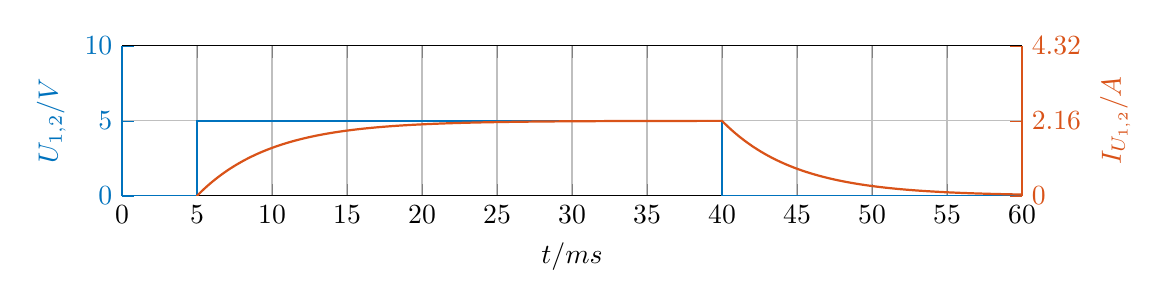
\begin{tikzpicture}
\pgfplotsset{
	width=4.5in,
	height=0.75in,
	every axis plot/.append style={thick}
}


\begin{axis}[%
scale only axis,
axis y line*=left,
ymin=0,
ymax=10,
xmin=0, xmax=60,
xlabel={$ t/ms $},
ytick={ 0, 5, 10},
ylabel style={font=\color{mycolor1}},
ylabel={$ U_{1,2}/V $},
ytick style={mycolor1},
yticklabel style={mycolor1},
y axis line style={mycolor1},
xmajorgrids,
ymajorgrids
]
\addplot[const plot, color=mycolor1] table[row sep=crcr] {%
-1	0\\
-0.99	0\\
-0.98	0\\
-0.97	0\\
-0.96	0\\
-0.95	0\\
-0.94	0\\
-0.93	0\\
-0.92	0\\
-0.91	0\\
-0.9	0\\
-0.89	0\\
-0.88	0\\
-0.87	0\\
-0.86	0\\
-0.85	0\\
-0.84	0\\
-0.83	0\\
-0.82	0\\
-0.81	0\\
-0.8	0\\
-0.79	0\\
-0.78	0\\
-0.77	0\\
-0.76	0\\
-0.75	0\\
-0.74	0\\
-0.73	0\\
-0.72	0\\
-0.71	0\\
-0.7	0\\
-0.69	0\\
-0.68	0\\
-0.67	0\\
-0.66	0\\
-0.65	0\\
-0.64	0\\
-0.63	0\\
-0.62	0\\
-0.61	0\\
-0.6	0\\
-0.59	0\\
-0.58	0\\
-0.57	0\\
-0.56	0\\
-0.55	0\\
-0.54	0\\
-0.53	0\\
-0.52	0\\
-0.51	0\\
-0.5	0\\
-0.49	0\\
-0.48	0\\
-0.47	0\\
-0.46	0\\
-0.45	0\\
-0.44	0\\
-0.43	0\\
-0.42	0\\
-0.41	0\\
-0.4	0\\
-0.39	0\\
-0.38	0\\
-0.37	0\\
-0.36	0\\
-0.35	0\\
-0.34	0\\
-0.33	0\\
-0.32	0\\
-0.31	0\\
-0.3	0\\
-0.29	0\\
-0.28	0\\
-0.27	0\\
-0.26	0\\
-0.25	0\\
-0.24	0\\
-0.23	0\\
-0.22	0\\
-0.21	0\\
-0.2	0\\
-0.19	0\\
-0.18	0\\
-0.17	0\\
-0.16	0\\
-0.15	0\\
-0.14	0\\
-0.13	0\\
-0.12	0\\
-0.11	0\\
-0.1	0\\
-0.09	0\\
-0.08	0\\
-0.07	0\\
-0.0599999999999999	0\\
-0.0499999999999999	0\\
-0.04	0\\
-0.03	0\\
-0.02	0\\
-0.01	0\\
0	0\\
0.01	0\\
0.02	0\\
0.03	0\\
0.04	0\\
0.05	0\\
0.0600000000000001	0\\
0.0700000000000001	0\\
0.0800000000000001	0\\
0.0900000000000001	0\\
0.1	0\\
0.11	0\\
0.12	0\\
0.13	0\\
0.14	0\\
0.15	0\\
0.16	0\\
0.17	0\\
0.18	0\\
0.19	0\\
0.2	0\\
0.21	0\\
0.22	0\\
0.23	0\\
0.24	0\\
0.25	0\\
0.26	0\\
0.27	0\\
0.28	0\\
0.29	0\\
0.3	0\\
0.31	0\\
0.32	0\\
0.33	0\\
0.34	0\\
0.35	0\\
0.36	0\\
0.37	0\\
0.38	0\\
0.39	0\\
0.4	0\\
0.41	0\\
0.42	0\\
0.43	0\\
0.44	0\\
0.45	0\\
0.46	0\\
0.47	0\\
0.48	0\\
0.49	0\\
0.5	0\\
0.51	0\\
0.52	0\\
0.53	0\\
0.54	0\\
0.55	0\\
0.56	0\\
0.57	0\\
0.58	0\\
0.59	0\\
0.6	0\\
0.61	0\\
0.62	0\\
0.63	0\\
0.64	0\\
0.65	0\\
0.66	0\\
0.67	0\\
0.68	0\\
0.69	0\\
0.7	0\\
0.71	0\\
0.72	0\\
0.73	0\\
0.74	0\\
0.75	0\\
0.76	0\\
0.77	0\\
0.78	0\\
0.79	0\\
0.8	0\\
0.81	0\\
0.82	0\\
0.83	0\\
0.84	0\\
0.85	0\\
0.86	0\\
0.87	0\\
0.88	0\\
0.89	0\\
0.9	0\\
0.91	0\\
0.92	0\\
0.93	0\\
0.94	0\\
0.95	0\\
0.96	0\\
0.97	0\\
0.98	0\\
0.99	0\\
1	0\\
1.01	0\\
1.02	0\\
1.03	0\\
1.04	0\\
1.05	0\\
1.06	0\\
1.07	0\\
1.08	0\\
1.09	0\\
1.1	0\\
1.11	0\\
1.12	0\\
1.13	0\\
1.14	0\\
1.15	0\\
1.16	0\\
1.17	0\\
1.18	0\\
1.19	0\\
1.2	0\\
1.21	0\\
1.22	0\\
1.23	0\\
1.24	0\\
1.25	0\\
1.26	0\\
1.27	0\\
1.28	0\\
1.29	0\\
1.3	0\\
1.31	0\\
1.32	0\\
1.33	0\\
1.34	0\\
1.35	0\\
1.36	0\\
1.37	0\\
1.38	0\\
1.39	0\\
1.4	0\\
1.41	0\\
1.42	0\\
1.43	0\\
1.44	0\\
1.45	0\\
1.46	0\\
1.47	0\\
1.48	0\\
1.49	0\\
1.5	0\\
1.51	0\\
1.52	0\\
1.53	0\\
1.54	0\\
1.55	0\\
1.56	0\\
1.57	0\\
1.58	0\\
1.59	0\\
1.6	0\\
1.61	0\\
1.62	0\\
1.63	0\\
1.64	0\\
1.65	0\\
1.66	0\\
1.67	0\\
1.68	0\\
1.69	0\\
1.7	0\\
1.71	0\\
1.72	0\\
1.73	0\\
1.74	0\\
1.75	0\\
1.76	0\\
1.77	0\\
1.78	0\\
1.79	0\\
1.8	0\\
1.81	0\\
1.82	0\\
1.83	0\\
1.84	0\\
1.85	0\\
1.86	0\\
1.87	0\\
1.88	0\\
1.89	0\\
1.9	0\\
1.91	0\\
1.92	0\\
1.93	0\\
1.94	0\\
1.95	0\\
1.96	0\\
1.97	0\\
1.98	0\\
1.99	0\\
2	0\\
2.01	0\\
2.02	0\\
2.03	0\\
2.04	0\\
2.05	0\\
2.06	0\\
2.07	0\\
2.08	0\\
2.09	0\\
2.1	0\\
2.11	0\\
2.12	0\\
2.13	0\\
2.14	0\\
2.15	0\\
2.16	0\\
2.17	0\\
2.18	0\\
2.19	0\\
2.2	0\\
2.21	0\\
2.22	0\\
2.23	0\\
2.24	0\\
2.25	0\\
2.26	0\\
2.27	0\\
2.28	0\\
2.29	0\\
2.3	0\\
2.31	0\\
2.32	0\\
2.33	0\\
2.34	0\\
2.35	0\\
2.36	0\\
2.37	0\\
2.38	0\\
2.39	0\\
2.4	0\\
2.41	0\\
2.42	0\\
2.43	0\\
2.44	0\\
2.45	0\\
2.46	0\\
2.47	0\\
2.48	0\\
2.49	0\\
2.5	0\\
2.51	0\\
2.52	0\\
2.53	0\\
2.54	0\\
2.55	0\\
2.56	0\\
2.57	0\\
2.58	0\\
2.59	0\\
2.6	0\\
2.61	0\\
2.62	0\\
2.63	0\\
2.64	0\\
2.65	0\\
2.66	0\\
2.67	0\\
2.68	0\\
2.69	0\\
2.7	0\\
2.71	0\\
2.72	0\\
2.73	0\\
2.74	0\\
2.75	0\\
2.76	0\\
2.77	0\\
2.78	0\\
2.79	0\\
2.8	0\\
2.81	0\\
2.82	0\\
2.83	0\\
2.84	0\\
2.85	0\\
2.86	0\\
2.87	0\\
2.88	0\\
2.89	0\\
2.9	0\\
2.91	0\\
2.92	0\\
2.93	0\\
2.94	0\\
2.95	0\\
2.96	0\\
2.97	0\\
2.98	0\\
2.99	0\\
3	0\\
3.01	0\\
3.02	0\\
3.03	0\\
3.04	0\\
3.05	0\\
3.06	0\\
3.07	0\\
3.08	0\\
3.09	0\\
3.1	0\\
3.11	0\\
3.12	0\\
3.13	0\\
3.14	0\\
3.15	0\\
3.16	0\\
3.17	0\\
3.18	0\\
3.19	0\\
3.2	0\\
3.21	0\\
3.22	0\\
3.23	0\\
3.24	0\\
3.25	0\\
3.26	0\\
3.27	0\\
3.28	0\\
3.29	0\\
3.3	0\\
3.31	0\\
3.32	0\\
3.33	0\\
3.34	0\\
3.35	0\\
3.36	0\\
3.37	0\\
3.38	0\\
3.39	0\\
3.4	0\\
3.41	0\\
3.42	0\\
3.43	0\\
3.44	0\\
3.45	0\\
3.46	0\\
3.47	0\\
3.48	0\\
3.49	0\\
3.5	0\\
3.51	0\\
3.52	0\\
3.53	0\\
3.54	0\\
3.55	0\\
3.56	0\\
3.57	0\\
3.58	0\\
3.59	0\\
3.6	0\\
3.61	0\\
3.62	0\\
3.63	0\\
3.64	0\\
3.65	0\\
3.66	0\\
3.67	0\\
3.68	0\\
3.69	0\\
3.7	0\\
3.71	0\\
3.72	0\\
3.73	0\\
3.74	0\\
3.75	0\\
3.76	0\\
3.77	0\\
3.78	0\\
3.79	0\\
3.8	0\\
3.81	0\\
3.82	0\\
3.83	0\\
3.84	0\\
3.85	0\\
3.86	0\\
3.87	0\\
3.88	0\\
3.89	0\\
3.9	0\\
3.91	0\\
3.92	0\\
3.93	0\\
3.94	0\\
3.95	0\\
3.96	0\\
3.97	0\\
3.98	0\\
3.99	0\\
4	0\\
4.01	0\\
4.02	0\\
4.03	0\\
4.04	0\\
4.05	0\\
4.06	0\\
4.07	0\\
4.08	0\\
4.09	0\\
4.1	0\\
4.11	0\\
4.12	0\\
4.13	0\\
4.14	0\\
4.15	0\\
4.16	0\\
4.17	0\\
4.18	0\\
4.19	0\\
4.2	0\\
4.21	0\\
4.22	0\\
4.23	0\\
4.24	0\\
4.25	0\\
4.26	0\\
4.27	0\\
4.28	0\\
4.29	0\\
4.3	0\\
4.31	0\\
4.32	0\\
4.33	0\\
4.34	0\\
4.35	0\\
4.36	0\\
4.37	0\\
4.38	0\\
4.39	0\\
4.4	0\\
4.41	0\\
4.42	0\\
4.43	0\\
4.44	0\\
4.45	0\\
4.46	0\\
4.47	0\\
4.48	0\\
4.49	0\\
4.5	0\\
4.51	0\\
4.52	0\\
4.53	0\\
4.54	0\\
4.55	0\\
4.56	0\\
4.57	0\\
4.58	0\\
4.59	0\\
4.6	0\\
4.61	0\\
4.62	0\\
4.63	0\\
4.64	0\\
4.65	0\\
4.66	0\\
4.67	0\\
4.68	0\\
4.69	0\\
4.7	0\\
4.71	0\\
4.72	0\\
4.73	0\\
4.74	0\\
4.75	0\\
4.76	0\\
4.77	0\\
4.78	0\\
4.79	0\\
4.8	0\\
4.81	0\\
4.82	0\\
4.83	0\\
4.84	0\\
4.85	0\\
4.86	0\\
4.87	0\\
4.88	0\\
4.89	0\\
4.9	0\\
4.91	0\\
4.92	0\\
4.93	0\\
4.94	0\\
4.95	0\\
4.96	0\\
4.97	0\\
4.98	0\\
4.99	0\\
5	5\\
5.01	5\\
5.02	5\\
5.03	5\\
5.04	5\\
5.05	5\\
5.06	5\\
5.07	5\\
5.08	5\\
5.09	5\\
5.1	5\\
5.11	5\\
5.12	5\\
5.13	5\\
5.14	5\\
5.15	5\\
5.16	5\\
5.17	5\\
5.18	5\\
5.19	5\\
5.2	5\\
5.21	5\\
5.22	5\\
5.23	5\\
5.24	5\\
5.25	5\\
5.26	5\\
5.27	5\\
5.28	5\\
5.29	5\\
5.3	5\\
5.31	5\\
5.32	5\\
5.33	5\\
5.34	5\\
5.35	5\\
5.36	5\\
5.37	5\\
5.38	5\\
5.39	5\\
5.4	5\\
5.41	5\\
5.42	5\\
5.43	5\\
5.44	5\\
5.45	5\\
5.46	5\\
5.47	5\\
5.48	5\\
5.49	5\\
5.5	5\\
5.51	5\\
5.52	5\\
5.53	5\\
5.54	5\\
5.55	5\\
5.56	5\\
5.57	5\\
5.58	5\\
5.59	5\\
5.6	5\\
5.61	5\\
5.62	5\\
5.63	5\\
5.64	5\\
5.65	5\\
5.66	5\\
5.67	5\\
5.68	5\\
5.69	5\\
5.7	5\\
5.71	5\\
5.72	5\\
5.73	5\\
5.74	5\\
5.75	5\\
5.76	5\\
5.77	5\\
5.78	5\\
5.79	5\\
5.8	5\\
5.81	5\\
5.82	5\\
5.83	5\\
5.84	5\\
5.85	5\\
5.86	5\\
5.87	5\\
5.88	5\\
5.89	5\\
5.9	5\\
5.91	5\\
5.92	5\\
5.93	5\\
5.94	5\\
5.95	5\\
5.96	5\\
5.97	5\\
5.98	5\\
5.99	5\\
6	5\\
6.01	5\\
6.02	5\\
6.03	5\\
6.04	5\\
6.05	5\\
6.06	5\\
6.07	5\\
6.08	5\\
6.09	5\\
6.1	5\\
6.11	5\\
6.12	5\\
6.13	5\\
6.14	5\\
6.15	5\\
6.16	5\\
6.17	5\\
6.18	5\\
6.19	5\\
6.2	5\\
6.21	5\\
6.22	5\\
6.23	5\\
6.24	5\\
6.25	5\\
6.26	5\\
6.27	5\\
6.28	5\\
6.29	5\\
6.3	5\\
6.31	5\\
6.32	5\\
6.33	5\\
6.34	5\\
6.35	5\\
6.36	5\\
6.37	5\\
6.38	5\\
6.39	5\\
6.4	5\\
6.41	5\\
6.42	5\\
6.43	5\\
6.44	5\\
6.45	5\\
6.46	5\\
6.47	5\\
6.48	5\\
6.49	5\\
6.5	5\\
6.51	5\\
6.52	5\\
6.53	5\\
6.54	5\\
6.55	5\\
6.56	5\\
6.57	5\\
6.58	5\\
6.59	5\\
6.6	5\\
6.61	5\\
6.62	5\\
6.63	5\\
6.64	5\\
6.65	5\\
6.66	5\\
6.67	5\\
6.68	5\\
6.69	5\\
6.7	5\\
6.71	5\\
6.72	5\\
6.73	5\\
6.74	5\\
6.75	5\\
6.76	5\\
6.77	5\\
6.78	5\\
6.79	5\\
6.8	5\\
6.81	5\\
6.82	5\\
6.83	5\\
6.84	5\\
6.85	5\\
6.86	5\\
6.87	5\\
6.88	5\\
6.89	5\\
6.9	5\\
6.91	5\\
6.92	5\\
6.93	5\\
6.94	5\\
6.95	5\\
6.96	5\\
6.97	5\\
6.98	5\\
6.99	5\\
7	5\\
7.01	5\\
7.02	5\\
7.03	5\\
7.04	5\\
7.05	5\\
7.06	5\\
7.07	5\\
7.08	5\\
7.09	5\\
7.1	5\\
7.11	5\\
7.12	5\\
7.13	5\\
7.14	5\\
7.15	5\\
7.16	5\\
7.17	5\\
7.18	5\\
7.19	5\\
7.2	5\\
7.21	5\\
7.22	5\\
7.23	5\\
7.24	5\\
7.25	5\\
7.26	5\\
7.27	5\\
7.28	5\\
7.29	5\\
7.3	5\\
7.31	5\\
7.32	5\\
7.33	5\\
7.34	5\\
7.35	5\\
7.36	5\\
7.37	5\\
7.38	5\\
7.39	5\\
7.4	5\\
7.41	5\\
7.42	5\\
7.43	5\\
7.44	5\\
7.45	5\\
7.46	5\\
7.47	5\\
7.48	5\\
7.49	5\\
7.5	5\\
7.51	5\\
7.52	5\\
7.53	5\\
7.54	5\\
7.55	5\\
7.56	5\\
7.57	5\\
7.58	5\\
7.59	5\\
7.6	5\\
7.61	5\\
7.62	5\\
7.63	5\\
7.64	5\\
7.65	5\\
7.66	5\\
7.67	5\\
7.68	5\\
7.69	5\\
7.7	5\\
7.71	5\\
7.72	5\\
7.73	5\\
7.74	5\\
7.75	5\\
7.76	5\\
7.77	5\\
7.78	5\\
7.79	5\\
7.8	5\\
7.81	5\\
7.82	5\\
7.83	5\\
7.84	5\\
7.85	5\\
7.86	5\\
7.87	5\\
7.88	5\\
7.89	5\\
7.9	5\\
7.91	5\\
7.92	5\\
7.93	5\\
7.94	5\\
7.95	5\\
7.96	5\\
7.97	5\\
7.98	5\\
7.99	5\\
8	5\\
8.01	5\\
8.02	5\\
8.03	5\\
8.04	5\\
8.05	5\\
8.06	5\\
8.07	5\\
8.08	5\\
8.09	5\\
8.1	5\\
8.11	5\\
8.12	5\\
8.13	5\\
8.14	5\\
8.15	5\\
8.16	5\\
8.17	5\\
8.18	5\\
8.19	5\\
8.2	5\\
8.21	5\\
8.22	5\\
8.23	5\\
8.24	5\\
8.25	5\\
8.26	5\\
8.27	5\\
8.28	5\\
8.29	5\\
8.3	5\\
8.31	5\\
8.32	5\\
8.33	5\\
8.34	5\\
8.35	5\\
8.36	5\\
8.37	5\\
8.38	5\\
8.39	5\\
8.4	5\\
8.41	5\\
8.42	5\\
8.43	5\\
8.44	5\\
8.45	5\\
8.46	5\\
8.47	5\\
8.48	5\\
8.49	5\\
8.5	5\\
8.51	5\\
8.52	5\\
8.53	5\\
8.54	5\\
8.55	5\\
8.56	5\\
8.57	5\\
8.58	5\\
8.59	5\\
8.6	5\\
8.61	5\\
8.62	5\\
8.63	5\\
8.64	5\\
8.65	5\\
8.66	5\\
8.67	5\\
8.68	5\\
8.69	5\\
8.7	5\\
8.71	5\\
8.72	5\\
8.73	5\\
8.74	5\\
8.75	5\\
8.76	5\\
8.77	5\\
8.78	5\\
8.79	5\\
8.8	5\\
8.81	5\\
8.82	5\\
8.83	5\\
8.84	5\\
8.85	5\\
8.86	5\\
8.87	5\\
8.88	5\\
8.89	5\\
8.9	5\\
8.91	5\\
8.92	5\\
8.93	5\\
8.94	5\\
8.95	5\\
8.96	5\\
8.97	5\\
8.98	5\\
8.99	5\\
9	5\\
9.01	5\\
9.02	5\\
9.03	5\\
9.04	5\\
9.05	5\\
9.06	5\\
9.07	5\\
9.08	5\\
9.09	5\\
9.1	5\\
9.11	5\\
9.12	5\\
9.13	5\\
9.14	5\\
9.15	5\\
9.16	5\\
9.17	5\\
9.18	5\\
9.19	5\\
9.2	5\\
9.21	5\\
9.22	5\\
9.23	5\\
9.24	5\\
9.25	5\\
9.26	5\\
9.27	5\\
9.28	5\\
9.29	5\\
9.3	5\\
9.31	5\\
9.32	5\\
9.33	5\\
9.34	5\\
9.35	5\\
9.36	5\\
9.37	5\\
9.38	5\\
9.39	5\\
9.4	5\\
9.41	5\\
9.42	5\\
9.43	5\\
9.44	5\\
9.45	5\\
9.46	5\\
9.47	5\\
9.48	5\\
9.49	5\\
9.5	5\\
9.51	5\\
9.52	5\\
9.53	5\\
9.54	5\\
9.55	5\\
9.56	5\\
9.57	5\\
9.58	5\\
9.59	5\\
9.6	5\\
9.61	5\\
9.62	5\\
9.63	5\\
9.64	5\\
9.65	5\\
9.66	5\\
9.67	5\\
9.68	5\\
9.69	5\\
9.7	5\\
9.71	5\\
9.72	5\\
9.73	5\\
9.74	5\\
9.75	5\\
9.76	5\\
9.77	5\\
9.78	5\\
9.79	5\\
9.8	5\\
9.81	5\\
9.82	5\\
9.83	5\\
9.84	5\\
9.85	5\\
9.86	5\\
9.87	5\\
9.88	5\\
9.89	5\\
9.9	5\\
9.91	5\\
9.92	5\\
9.93	5\\
9.94	5\\
9.95	5\\
9.96	5\\
9.97	5\\
9.98	5\\
9.99	5\\
10	5\\
10.01	5\\
10.02	5\\
10.03	5\\
10.04	5\\
10.05	5\\
10.06	5\\
10.07	5\\
10.08	5\\
10.09	5\\
10.1	5\\
10.11	5\\
10.12	5\\
10.13	5\\
10.14	5\\
10.15	5\\
10.16	5\\
10.17	5\\
10.18	5\\
10.19	5\\
10.2	5\\
10.21	5\\
10.22	5\\
10.23	5\\
10.24	5\\
10.25	5\\
10.26	5\\
10.27	5\\
10.28	5\\
10.29	5\\
10.3	5\\
10.31	5\\
10.32	5\\
10.33	5\\
10.34	5\\
10.35	5\\
10.36	5\\
10.37	5\\
10.38	5\\
10.39	5\\
10.4	5\\
10.41	5\\
10.42	5\\
10.43	5\\
10.44	5\\
10.45	5\\
10.46	5\\
10.47	5\\
10.48	5\\
10.49	5\\
10.5	5\\
10.51	5\\
10.52	5\\
10.53	5\\
10.54	5\\
10.55	5\\
10.56	5\\
10.57	5\\
10.58	5\\
10.59	5\\
10.6	5\\
10.61	5\\
10.62	5\\
10.63	5\\
10.64	5\\
10.65	5\\
10.66	5\\
10.67	5\\
10.68	5\\
10.69	5\\
10.7	5\\
10.71	5\\
10.72	5\\
10.73	5\\
10.74	5\\
10.75	5\\
10.76	5\\
10.77	5\\
10.78	5\\
10.79	5\\
10.8	5\\
10.81	5\\
10.82	5\\
10.83	5\\
10.84	5\\
10.85	5\\
10.86	5\\
10.87	5\\
10.88	5\\
10.89	5\\
10.9	5\\
10.91	5\\
10.92	5\\
10.93	5\\
10.94	5\\
10.95	5\\
10.96	5\\
10.97	5\\
10.98	5\\
10.99	5\\
11	5\\
11.01	5\\
11.02	5\\
11.03	5\\
11.04	5\\
11.05	5\\
11.06	5\\
11.07	5\\
11.08	5\\
11.09	5\\
11.1	5\\
11.11	5\\
11.12	5\\
11.13	5\\
11.14	5\\
11.15	5\\
11.16	5\\
11.17	5\\
11.18	5\\
11.19	5\\
11.2	5\\
11.21	5\\
11.22	5\\
11.23	5\\
11.24	5\\
11.25	5\\
11.26	5\\
11.27	5\\
11.28	5\\
11.29	5\\
11.3	5\\
11.31	5\\
11.32	5\\
11.33	5\\
11.34	5\\
11.35	5\\
11.36	5\\
11.37	5\\
11.38	5\\
11.39	5\\
11.4	5\\
11.41	5\\
11.42	5\\
11.43	5\\
11.44	5\\
11.45	5\\
11.46	5\\
11.47	5\\
11.48	5\\
11.49	5\\
11.5	5\\
11.51	5\\
11.52	5\\
11.53	5\\
11.54	5\\
11.55	5\\
11.56	5\\
11.57	5\\
11.58	5\\
11.59	5\\
11.6	5\\
11.61	5\\
11.62	5\\
11.63	5\\
11.64	5\\
11.65	5\\
11.66	5\\
11.67	5\\
11.68	5\\
11.69	5\\
11.7	5\\
11.71	5\\
11.72	5\\
11.73	5\\
11.74	5\\
11.75	5\\
11.76	5\\
11.77	5\\
11.78	5\\
11.79	5\\
11.8	5\\
11.81	5\\
11.82	5\\
11.83	5\\
11.84	5\\
11.85	5\\
11.86	5\\
11.87	5\\
11.88	5\\
11.89	5\\
11.9	5\\
11.91	5\\
11.92	5\\
11.93	5\\
11.94	5\\
11.95	5\\
11.96	5\\
11.97	5\\
11.98	5\\
11.99	5\\
12	5\\
12.01	5\\
12.02	5\\
12.03	5\\
12.04	5\\
12.05	5\\
12.06	5\\
12.07	5\\
12.08	5\\
12.09	5\\
12.1	5\\
12.11	5\\
12.12	5\\
12.13	5\\
12.14	5\\
12.15	5\\
12.16	5\\
12.17	5\\
12.18	5\\
12.19	5\\
12.2	5\\
12.21	5\\
12.22	5\\
12.23	5\\
12.24	5\\
12.25	5\\
12.26	5\\
12.27	5\\
12.28	5\\
12.29	5\\
12.3	5\\
12.31	5\\
12.32	5\\
12.33	5\\
12.34	5\\
12.35	5\\
12.36	5\\
12.37	5\\
12.38	5\\
12.39	5\\
12.4	5\\
12.41	5\\
12.42	5\\
12.43	5\\
12.44	5\\
12.45	5\\
12.46	5\\
12.47	5\\
12.48	5\\
12.49	5\\
12.5	5\\
12.51	5\\
12.52	5\\
12.53	5\\
12.54	5\\
12.55	5\\
12.56	5\\
12.57	5\\
12.58	5\\
12.59	5\\
12.6	5\\
12.61	5\\
12.62	5\\
12.63	5\\
12.64	5\\
12.65	5\\
12.66	5\\
12.67	5\\
12.68	5\\
12.69	5\\
12.7	5\\
12.71	5\\
12.72	5\\
12.73	5\\
12.74	5\\
12.75	5\\
12.76	5\\
12.77	5\\
12.78	5\\
12.79	5\\
12.8	5\\
12.81	5\\
12.82	5\\
12.83	5\\
12.84	5\\
12.85	5\\
12.86	5\\
12.87	5\\
12.88	5\\
12.89	5\\
12.9	5\\
12.91	5\\
12.92	5\\
12.93	5\\
12.94	5\\
12.95	5\\
12.96	5\\
12.97	5\\
12.98	5\\
12.99	5\\
13	5\\
13.01	5\\
13.02	5\\
13.03	5\\
13.04	5\\
13.05	5\\
13.06	5\\
13.07	5\\
13.08	5\\
13.09	5\\
13.1	5\\
13.11	5\\
13.12	5\\
13.13	5\\
13.14	5\\
13.15	5\\
13.16	5\\
13.17	5\\
13.18	5\\
13.19	5\\
13.2	5\\
13.21	5\\
13.22	5\\
13.23	5\\
13.24	5\\
13.25	5\\
13.26	5\\
13.27	5\\
13.28	5\\
13.29	5\\
13.3	5\\
13.31	5\\
13.32	5\\
13.33	5\\
13.34	5\\
13.35	5\\
13.36	5\\
13.37	5\\
13.38	5\\
13.39	5\\
13.4	5\\
13.41	5\\
13.42	5\\
13.43	5\\
13.44	5\\
13.45	5\\
13.46	5\\
13.47	5\\
13.48	5\\
13.49	5\\
13.5	5\\
13.51	5\\
13.52	5\\
13.53	5\\
13.54	5\\
13.55	5\\
13.56	5\\
13.57	5\\
13.58	5\\
13.59	5\\
13.6	5\\
13.61	5\\
13.62	5\\
13.63	5\\
13.64	5\\
13.65	5\\
13.66	5\\
13.67	5\\
13.68	5\\
13.69	5\\
13.7	5\\
13.71	5\\
13.72	5\\
13.73	5\\
13.74	5\\
13.75	5\\
13.76	5\\
13.77	5\\
13.78	5\\
13.79	5\\
13.8	5\\
13.81	5\\
13.82	5\\
13.83	5\\
13.84	5\\
13.85	5\\
13.86	5\\
13.87	5\\
13.88	5\\
13.89	5\\
13.9	5\\
13.91	5\\
13.92	5\\
13.93	5\\
13.94	5\\
13.95	5\\
13.96	5\\
13.97	5\\
13.98	5\\
13.99	5\\
14	5\\
14.01	5\\
14.02	5\\
14.03	5\\
14.04	5\\
14.05	5\\
14.06	5\\
14.07	5\\
14.08	5\\
14.09	5\\
14.1	5\\
14.11	5\\
14.12	5\\
14.13	5\\
14.14	5\\
14.15	5\\
14.16	5\\
14.17	5\\
14.18	5\\
14.19	5\\
14.2	5\\
14.21	5\\
14.22	5\\
14.23	5\\
14.24	5\\
14.25	5\\
14.26	5\\
14.27	5\\
14.28	5\\
14.29	5\\
14.3	5\\
14.31	5\\
14.32	5\\
14.33	5\\
14.34	5\\
14.35	5\\
14.36	5\\
14.37	5\\
14.38	5\\
14.39	5\\
14.4	5\\
14.41	5\\
14.42	5\\
14.43	5\\
14.44	5\\
14.45	5\\
14.46	5\\
14.47	5\\
14.48	5\\
14.49	5\\
14.5	5\\
14.51	5\\
14.52	5\\
14.53	5\\
14.54	5\\
14.55	5\\
14.56	5\\
14.57	5\\
14.58	5\\
14.59	5\\
14.6	5\\
14.61	5\\
14.62	5\\
14.63	5\\
14.64	5\\
14.65	5\\
14.66	5\\
14.67	5\\
14.68	5\\
14.69	5\\
14.7	5\\
14.71	5\\
14.72	5\\
14.73	5\\
14.74	5\\
14.75	5\\
14.76	5\\
14.77	5\\
14.78	5\\
14.79	5\\
14.8	5\\
14.81	5\\
14.82	5\\
14.83	5\\
14.84	5\\
14.85	5\\
14.86	5\\
14.87	5\\
14.88	5\\
14.89	5\\
14.9	5\\
14.91	5\\
14.92	5\\
14.93	5\\
14.94	5\\
14.95	5\\
14.96	5\\
14.97	5\\
14.98	5\\
14.99	5\\
15	5\\
15.01	5\\
15.02	5\\
15.03	5\\
15.04	5\\
15.05	5\\
15.06	5\\
15.07	5\\
15.08	5\\
15.09	5\\
15.1	5\\
15.11	5\\
15.12	5\\
15.13	5\\
15.14	5\\
15.15	5\\
15.16	5\\
15.17	5\\
15.18	5\\
15.19	5\\
15.2	5\\
15.21	5\\
15.22	5\\
15.23	5\\
15.24	5\\
15.25	5\\
15.26	5\\
15.27	5\\
15.28	5\\
15.29	5\\
15.3	5\\
15.31	5\\
15.32	5\\
15.33	5\\
15.34	5\\
15.35	5\\
15.36	5\\
15.37	5\\
15.38	5\\
15.39	5\\
15.4	5\\
15.41	5\\
15.42	5\\
15.43	5\\
15.44	5\\
15.45	5\\
15.46	5\\
15.47	5\\
15.48	5\\
15.49	5\\
15.5	5\\
15.51	5\\
15.52	5\\
15.53	5\\
15.54	5\\
15.55	5\\
15.56	5\\
15.57	5\\
15.58	5\\
15.59	5\\
15.6	5\\
15.61	5\\
15.62	5\\
15.63	5\\
15.64	5\\
15.65	5\\
15.66	5\\
15.67	5\\
15.68	5\\
15.69	5\\
15.7	5\\
15.71	5\\
15.72	5\\
15.73	5\\
15.74	5\\
15.75	5\\
15.76	5\\
15.77	5\\
15.78	5\\
15.79	5\\
15.8	5\\
15.81	5\\
15.82	5\\
15.83	5\\
15.84	5\\
15.85	5\\
15.86	5\\
15.87	5\\
15.88	5\\
15.89	5\\
15.9	5\\
15.91	5\\
15.92	5\\
15.93	5\\
15.94	5\\
15.95	5\\
15.96	5\\
15.97	5\\
15.98	5\\
15.99	5\\
16	5\\
16.01	5\\
16.02	5\\
16.03	5\\
16.04	5\\
16.05	5\\
16.06	5\\
16.07	5\\
16.08	5\\
16.09	5\\
16.1	5\\
16.11	5\\
16.12	5\\
16.13	5\\
16.14	5\\
16.15	5\\
16.16	5\\
16.17	5\\
16.18	5\\
16.19	5\\
16.2	5\\
16.21	5\\
16.22	5\\
16.23	5\\
16.24	5\\
16.25	5\\
16.26	5\\
16.27	5\\
16.28	5\\
16.29	5\\
16.3	5\\
16.31	5\\
16.32	5\\
16.33	5\\
16.34	5\\
16.35	5\\
16.36	5\\
16.37	5\\
16.38	5\\
16.39	5\\
16.4	5\\
16.41	5\\
16.42	5\\
16.43	5\\
16.44	5\\
16.45	5\\
16.46	5\\
16.47	5\\
16.48	5\\
16.49	5\\
16.5	5\\
16.51	5\\
16.52	5\\
16.53	5\\
16.54	5\\
16.55	5\\
16.56	5\\
16.57	5\\
16.58	5\\
16.59	5\\
16.6	5\\
16.61	5\\
16.62	5\\
16.63	5\\
16.64	5\\
16.65	5\\
16.66	5\\
16.67	5\\
16.68	5\\
16.69	5\\
16.7	5\\
16.71	5\\
16.72	5\\
16.73	5\\
16.74	5\\
16.75	5\\
16.76	5\\
16.77	5\\
16.78	5\\
16.79	5\\
16.8	5\\
16.81	5\\
16.82	5\\
16.83	5\\
16.84	5\\
16.85	5\\
16.86	5\\
16.87	5\\
16.88	5\\
16.89	5\\
16.9	5\\
16.91	5\\
16.92	5\\
16.93	5\\
16.94	5\\
16.95	5\\
16.96	5\\
16.97	5\\
16.98	5\\
16.99	5\\
17	5\\
17.01	5\\
17.02	5\\
17.03	5\\
17.04	5\\
17.05	5\\
17.06	5\\
17.07	5\\
17.08	5\\
17.09	5\\
17.1	5\\
17.11	5\\
17.12	5\\
17.13	5\\
17.14	5\\
17.15	5\\
17.16	5\\
17.17	5\\
17.18	5\\
17.19	5\\
17.2	5\\
17.21	5\\
17.22	5\\
17.23	5\\
17.24	5\\
17.25	5\\
17.26	5\\
17.27	5\\
17.28	5\\
17.29	5\\
17.3	5\\
17.31	5\\
17.32	5\\
17.33	5\\
17.34	5\\
17.35	5\\
17.36	5\\
17.37	5\\
17.38	5\\
17.39	5\\
17.4	5\\
17.41	5\\
17.42	5\\
17.43	5\\
17.44	5\\
17.45	5\\
17.46	5\\
17.47	5\\
17.48	5\\
17.49	5\\
17.5	5\\
17.51	5\\
17.52	5\\
17.53	5\\
17.54	5\\
17.55	5\\
17.56	5\\
17.57	5\\
17.58	5\\
17.59	5\\
17.6	5\\
17.61	5\\
17.62	5\\
17.63	5\\
17.64	5\\
17.65	5\\
17.66	5\\
17.67	5\\
17.68	5\\
17.69	5\\
17.7	5\\
17.71	5\\
17.72	5\\
17.73	5\\
17.74	5\\
17.75	5\\
17.76	5\\
17.77	5\\
17.78	5\\
17.79	5\\
17.8	5\\
17.81	5\\
17.82	5\\
17.83	5\\
17.84	5\\
17.85	5\\
17.86	5\\
17.87	5\\
17.88	5\\
17.89	5\\
17.9	5\\
17.91	5\\
17.92	5\\
17.93	5\\
17.94	5\\
17.95	5\\
17.96	5\\
17.97	5\\
17.98	5\\
17.99	5\\
18	5\\
18.01	5\\
18.02	5\\
18.03	5\\
18.04	5\\
18.05	5\\
18.06	5\\
18.07	5\\
18.08	5\\
18.09	5\\
18.1	5\\
18.11	5\\
18.12	5\\
18.13	5\\
18.14	5\\
18.15	5\\
18.16	5\\
18.17	5\\
18.18	5\\
18.19	5\\
18.2	5\\
18.21	5\\
18.22	5\\
18.23	5\\
18.24	5\\
18.25	5\\
18.26	5\\
18.27	5\\
18.28	5\\
18.29	5\\
18.3	5\\
18.31	5\\
18.32	5\\
18.33	5\\
18.34	5\\
18.35	5\\
18.36	5\\
18.37	5\\
18.38	5\\
18.39	5\\
18.4	5\\
18.41	5\\
18.42	5\\
18.43	5\\
18.44	5\\
18.45	5\\
18.46	5\\
18.47	5\\
18.48	5\\
18.49	5\\
18.5	5\\
18.51	5\\
18.52	5\\
18.53	5\\
18.54	5\\
18.55	5\\
18.56	5\\
18.57	5\\
18.58	5\\
18.59	5\\
18.6	5\\
18.61	5\\
18.62	5\\
18.63	5\\
18.64	5\\
18.65	5\\
18.66	5\\
18.67	5\\
18.68	5\\
18.69	5\\
18.7	5\\
18.71	5\\
18.72	5\\
18.73	5\\
18.74	5\\
18.75	5\\
18.76	5\\
18.77	5\\
18.78	5\\
18.79	5\\
18.8	5\\
18.81	5\\
18.82	5\\
18.83	5\\
18.84	5\\
18.85	5\\
18.86	5\\
18.87	5\\
18.88	5\\
18.89	5\\
18.9	5\\
18.91	5\\
18.92	5\\
18.93	5\\
18.94	5\\
18.95	5\\
18.96	5\\
18.97	5\\
18.98	5\\
18.99	5\\
19	5\\
19.01	5\\
19.02	5\\
19.03	5\\
19.04	5\\
19.05	5\\
19.06	5\\
19.07	5\\
19.08	5\\
19.09	5\\
19.1	5\\
19.11	5\\
19.12	5\\
19.13	5\\
19.14	5\\
19.15	5\\
19.16	5\\
19.17	5\\
19.18	5\\
19.19	5\\
19.2	5\\
19.21	5\\
19.22	5\\
19.23	5\\
19.24	5\\
19.25	5\\
19.26	5\\
19.27	5\\
19.28	5\\
19.29	5\\
19.3	5\\
19.31	5\\
19.32	5\\
19.33	5\\
19.34	5\\
19.35	5\\
19.36	5\\
19.37	5\\
19.38	5\\
19.39	5\\
19.4	5\\
19.41	5\\
19.42	5\\
19.43	5\\
19.44	5\\
19.45	5\\
19.46	5\\
19.47	5\\
19.48	5\\
19.49	5\\
19.5	5\\
19.51	5\\
19.52	5\\
19.53	5\\
19.54	5\\
19.55	5\\
19.56	5\\
19.57	5\\
19.58	5\\
19.59	5\\
19.6	5\\
19.61	5\\
19.62	5\\
19.63	5\\
19.64	5\\
19.65	5\\
19.66	5\\
19.67	5\\
19.68	5\\
19.69	5\\
19.7	5\\
19.71	5\\
19.72	5\\
19.73	5\\
19.74	5\\
19.75	5\\
19.76	5\\
19.77	5\\
19.78	5\\
19.79	5\\
19.8	5\\
19.81	5\\
19.82	5\\
19.83	5\\
19.84	5\\
19.85	5\\
19.86	5\\
19.87	5\\
19.88	5\\
19.89	5\\
19.9	5\\
19.91	5\\
19.92	5\\
19.93	5\\
19.94	5\\
19.95	5\\
19.96	5\\
19.97	5\\
19.98	5\\
19.99	5\\
20	5\\
20.01	5\\
20.02	5\\
20.03	5\\
20.04	5\\
20.05	5\\
20.06	5\\
20.07	5\\
20.08	5\\
20.09	5\\
20.1	5\\
20.11	5\\
20.12	5\\
20.13	5\\
20.14	5\\
20.15	5\\
20.16	5\\
20.17	5\\
20.18	5\\
20.19	5\\
20.2	5\\
20.21	5\\
20.22	5\\
20.23	5\\
20.24	5\\
20.25	5\\
20.26	5\\
20.27	5\\
20.28	5\\
20.29	5\\
20.3	5\\
20.31	5\\
20.32	5\\
20.33	5\\
20.34	5\\
20.35	5\\
20.36	5\\
20.37	5\\
20.38	5\\
20.39	5\\
20.4	5\\
20.41	5\\
20.42	5\\
20.43	5\\
20.44	5\\
20.45	5\\
20.46	5\\
20.47	5\\
20.48	5\\
20.49	5\\
20.5	5\\
20.51	5\\
20.52	5\\
20.53	5\\
20.54	5\\
20.55	5\\
20.56	5\\
20.57	5\\
20.58	5\\
20.59	5\\
20.6	5\\
20.61	5\\
20.62	5\\
20.63	5\\
20.64	5\\
20.65	5\\
20.66	5\\
20.67	5\\
20.68	5\\
20.69	5\\
20.7	5\\
20.71	5\\
20.72	5\\
20.73	5\\
20.74	5\\
20.75	5\\
20.76	5\\
20.77	5\\
20.78	5\\
20.79	5\\
20.8	5\\
20.81	5\\
20.82	5\\
20.83	5\\
20.84	5\\
20.85	5\\
20.86	5\\
20.87	5\\
20.88	5\\
20.89	5\\
20.9	5\\
20.91	5\\
20.92	5\\
20.93	5\\
20.94	5\\
20.95	5\\
20.96	5\\
20.97	5\\
20.98	5\\
20.99	5\\
21	5\\
21.01	5\\
21.02	5\\
21.03	5\\
21.04	5\\
21.05	5\\
21.06	5\\
21.07	5\\
21.08	5\\
21.09	5\\
21.1	5\\
21.11	5\\
21.12	5\\
21.13	5\\
21.14	5\\
21.15	5\\
21.16	5\\
21.17	5\\
21.18	5\\
21.19	5\\
21.2	5\\
21.21	5\\
21.22	5\\
21.23	5\\
21.24	5\\
21.25	5\\
21.26	5\\
21.27	5\\
21.28	5\\
21.29	5\\
21.3	5\\
21.31	5\\
21.32	5\\
21.33	5\\
21.34	5\\
21.35	5\\
21.36	5\\
21.37	5\\
21.38	5\\
21.39	5\\
21.4	5\\
21.41	5\\
21.42	5\\
21.43	5\\
21.44	5\\
21.45	5\\
21.46	5\\
21.47	5\\
21.48	5\\
21.49	5\\
21.5	5\\
21.51	5\\
21.52	5\\
21.53	5\\
21.54	5\\
21.55	5\\
21.56	5\\
21.57	5\\
21.58	5\\
21.59	5\\
21.6	5\\
21.61	5\\
21.62	5\\
21.63	5\\
21.64	5\\
21.65	5\\
21.66	5\\
21.67	5\\
21.68	5\\
21.69	5\\
21.7	5\\
21.71	5\\
21.72	5\\
21.73	5\\
21.74	5\\
21.75	5\\
21.76	5\\
21.77	5\\
21.78	5\\
21.79	5\\
21.8	5\\
21.81	5\\
21.82	5\\
21.83	5\\
21.84	5\\
21.85	5\\
21.86	5\\
21.87	5\\
21.88	5\\
21.89	5\\
21.9	5\\
21.91	5\\
21.92	5\\
21.93	5\\
21.94	5\\
21.95	5\\
21.96	5\\
21.97	5\\
21.98	5\\
21.99	5\\
22	5\\
22.01	5\\
22.02	5\\
22.03	5\\
22.04	5\\
22.05	5\\
22.06	5\\
22.07	5\\
22.08	5\\
22.09	5\\
22.1	5\\
22.11	5\\
22.12	5\\
22.13	5\\
22.14	5\\
22.15	5\\
22.16	5\\
22.17	5\\
22.18	5\\
22.19	5\\
22.2	5\\
22.21	5\\
22.22	5\\
22.23	5\\
22.24	5\\
22.25	5\\
22.26	5\\
22.27	5\\
22.28	5\\
22.29	5\\
22.3	5\\
22.31	5\\
22.32	5\\
22.33	5\\
22.34	5\\
22.35	5\\
22.36	5\\
22.37	5\\
22.38	5\\
22.39	5\\
22.4	5\\
22.41	5\\
22.42	5\\
22.43	5\\
22.44	5\\
22.45	5\\
22.46	5\\
22.47	5\\
22.48	5\\
22.49	5\\
22.5	5\\
22.51	5\\
22.52	5\\
22.53	5\\
22.54	5\\
22.55	5\\
22.56	5\\
22.57	5\\
22.58	5\\
22.59	5\\
22.6	5\\
22.61	5\\
22.62	5\\
22.63	5\\
22.64	5\\
22.65	5\\
22.66	5\\
22.67	5\\
22.68	5\\
22.69	5\\
22.7	5\\
22.71	5\\
22.72	5\\
22.73	5\\
22.74	5\\
22.75	5\\
22.76	5\\
22.77	5\\
22.78	5\\
22.79	5\\
22.8	5\\
22.81	5\\
22.82	5\\
22.83	5\\
22.84	5\\
22.85	5\\
22.86	5\\
22.87	5\\
22.88	5\\
22.89	5\\
22.9	5\\
22.91	5\\
22.92	5\\
22.93	5\\
22.94	5\\
22.95	5\\
22.96	5\\
22.97	5\\
22.98	5\\
22.99	5\\
23	5\\
23.01	5\\
23.02	5\\
23.03	5\\
23.04	5\\
23.05	5\\
23.06	5\\
23.07	5\\
23.08	5\\
23.09	5\\
23.1	5\\
23.11	5\\
23.12	5\\
23.13	5\\
23.14	5\\
23.15	5\\
23.16	5\\
23.17	5\\
23.18	5\\
23.19	5\\
23.2	5\\
23.21	5\\
23.22	5\\
23.23	5\\
23.24	5\\
23.25	5\\
23.26	5\\
23.27	5\\
23.28	5\\
23.29	5\\
23.3	5\\
23.31	5\\
23.32	5\\
23.33	5\\
23.34	5\\
23.35	5\\
23.36	5\\
23.37	5\\
23.38	5\\
23.39	5\\
23.4	5\\
23.41	5\\
23.42	5\\
23.43	5\\
23.44	5\\
23.45	5\\
23.46	5\\
23.47	5\\
23.48	5\\
23.49	5\\
23.5	5\\
23.51	5\\
23.52	5\\
23.53	5\\
23.54	5\\
23.55	5\\
23.56	5\\
23.57	5\\
23.58	5\\
23.59	5\\
23.6	5\\
23.61	5\\
23.62	5\\
23.63	5\\
23.64	5\\
23.65	5\\
23.66	5\\
23.67	5\\
23.68	5\\
23.69	5\\
23.7	5\\
23.71	5\\
23.72	5\\
23.73	5\\
23.74	5\\
23.75	5\\
23.76	5\\
23.77	5\\
23.78	5\\
23.79	5\\
23.8	5\\
23.81	5\\
23.82	5\\
23.83	5\\
23.84	5\\
23.85	5\\
23.86	5\\
23.87	5\\
23.88	5\\
23.89	5\\
23.9	5\\
23.91	5\\
23.92	5\\
23.93	5\\
23.94	5\\
23.95	5\\
23.96	5\\
23.97	5\\
23.98	5\\
23.99	5\\
24	5\\
24.01	5\\
24.02	5\\
24.03	5\\
24.04	5\\
24.05	5\\
24.06	5\\
24.07	5\\
24.08	5\\
24.09	5\\
24.1	5\\
24.11	5\\
24.12	5\\
24.13	5\\
24.14	5\\
24.15	5\\
24.16	5\\
24.17	5\\
24.18	5\\
24.19	5\\
24.2	5\\
24.21	5\\
24.22	5\\
24.23	5\\
24.24	5\\
24.25	5\\
24.26	5\\
24.27	5\\
24.28	5\\
24.29	5\\
24.3	5\\
24.31	5\\
24.32	5\\
24.33	5\\
24.34	5\\
24.35	5\\
24.36	5\\
24.37	5\\
24.38	5\\
24.39	5\\
24.4	5\\
24.41	5\\
24.42	5\\
24.43	5\\
24.44	5\\
24.45	5\\
24.46	5\\
24.47	5\\
24.48	5\\
24.49	5\\
24.5	5\\
24.51	5\\
24.52	5\\
24.53	5\\
24.54	5\\
24.55	5\\
24.56	5\\
24.57	5\\
24.58	5\\
24.59	5\\
24.6	5\\
24.61	5\\
24.62	5\\
24.63	5\\
24.64	5\\
24.65	5\\
24.66	5\\
24.67	5\\
24.68	5\\
24.69	5\\
24.7	5\\
24.71	5\\
24.72	5\\
24.73	5\\
24.74	5\\
24.75	5\\
24.76	5\\
24.77	5\\
24.78	5\\
24.79	5\\
24.8	5\\
24.81	5\\
24.82	5\\
24.83	5\\
24.84	5\\
24.85	5\\
24.86	5\\
24.87	5\\
24.88	5\\
24.89	5\\
24.9	5\\
24.91	5\\
24.92	5\\
24.93	5\\
24.94	5\\
24.95	5\\
24.96	5\\
24.97	5\\
24.98	5\\
24.99	5\\
25	5\\
25.01	5\\
25.02	5\\
25.03	5\\
25.04	5\\
25.05	5\\
25.06	5\\
25.07	5\\
25.08	5\\
25.09	5\\
25.1	5\\
25.11	5\\
25.12	5\\
25.13	5\\
25.14	5\\
25.15	5\\
25.16	5\\
25.17	5\\
25.18	5\\
25.19	5\\
25.2	5\\
25.21	5\\
25.22	5\\
25.23	5\\
25.24	5\\
25.25	5\\
25.26	5\\
25.27	5\\
25.28	5\\
25.29	5\\
25.3	5\\
25.31	5\\
25.32	5\\
25.33	5\\
25.34	5\\
25.35	5\\
25.36	5\\
25.37	5\\
25.38	5\\
25.39	5\\
25.4	5\\
25.41	5\\
25.42	5\\
25.43	5\\
25.44	5\\
25.45	5\\
25.46	5\\
25.47	5\\
25.48	5\\
25.49	5\\
25.5	5\\
25.51	5\\
25.52	5\\
25.53	5\\
25.54	5\\
25.55	5\\
25.56	5\\
25.57	5\\
25.58	5\\
25.59	5\\
25.6	5\\
25.61	5\\
25.62	5\\
25.63	5\\
25.64	5\\
25.65	5\\
25.66	5\\
25.67	5\\
25.68	5\\
25.69	5\\
25.7	5\\
25.71	5\\
25.72	5\\
25.73	5\\
25.74	5\\
25.75	5\\
25.76	5\\
25.77	5\\
25.78	5\\
25.79	5\\
25.8	5\\
25.81	5\\
25.82	5\\
25.83	5\\
25.84	5\\
25.85	5\\
25.86	5\\
25.87	5\\
25.88	5\\
25.89	5\\
25.9	5\\
25.91	5\\
25.92	5\\
25.93	5\\
25.94	5\\
25.95	5\\
25.96	5\\
25.97	5\\
25.98	5\\
25.99	5\\
26	5\\
26.01	5\\
26.02	5\\
26.03	5\\
26.04	5\\
26.05	5\\
26.06	5\\
26.07	5\\
26.08	5\\
26.09	5\\
26.1	5\\
26.11	5\\
26.12	5\\
26.13	5\\
26.14	5\\
26.15	5\\
26.16	5\\
26.17	5\\
26.18	5\\
26.19	5\\
26.2	5\\
26.21	5\\
26.22	5\\
26.23	5\\
26.24	5\\
26.25	5\\
26.26	5\\
26.27	5\\
26.28	5\\
26.29	5\\
26.3	5\\
26.31	5\\
26.32	5\\
26.33	5\\
26.34	5\\
26.35	5\\
26.36	5\\
26.37	5\\
26.38	5\\
26.39	5\\
26.4	5\\
26.41	5\\
26.42	5\\
26.43	5\\
26.44	5\\
26.45	5\\
26.46	5\\
26.47	5\\
26.48	5\\
26.49	5\\
26.5	5\\
26.51	5\\
26.52	5\\
26.53	5\\
26.54	5\\
26.55	5\\
26.56	5\\
26.57	5\\
26.58	5\\
26.59	5\\
26.6	5\\
26.61	5\\
26.62	5\\
26.63	5\\
26.64	5\\
26.65	5\\
26.66	5\\
26.67	5\\
26.68	5\\
26.69	5\\
26.7	5\\
26.71	5\\
26.72	5\\
26.73	5\\
26.74	5\\
26.75	5\\
26.76	5\\
26.77	5\\
26.78	5\\
26.79	5\\
26.8	5\\
26.81	5\\
26.82	5\\
26.83	5\\
26.84	5\\
26.85	5\\
26.86	5\\
26.87	5\\
26.88	5\\
26.89	5\\
26.9	5\\
26.91	5\\
26.92	5\\
26.93	5\\
26.94	5\\
26.95	5\\
26.96	5\\
26.97	5\\
26.98	5\\
26.99	5\\
27	5\\
27.01	5\\
27.02	5\\
27.03	5\\
27.04	5\\
27.05	5\\
27.06	5\\
27.07	5\\
27.08	5\\
27.09	5\\
27.1	5\\
27.11	5\\
27.12	5\\
27.13	5\\
27.14	5\\
27.15	5\\
27.16	5\\
27.17	5\\
27.18	5\\
27.19	5\\
27.2	5\\
27.21	5\\
27.22	5\\
27.23	5\\
27.24	5\\
27.25	5\\
27.26	5\\
27.27	5\\
27.28	5\\
27.29	5\\
27.3	5\\
27.31	5\\
27.32	5\\
27.33	5\\
27.34	5\\
27.35	5\\
27.36	5\\
27.37	5\\
27.38	5\\
27.39	5\\
27.4	5\\
27.41	5\\
27.42	5\\
27.43	5\\
27.44	5\\
27.45	5\\
27.46	5\\
27.47	5\\
27.48	5\\
27.49	5\\
27.5	5\\
27.51	5\\
27.52	5\\
27.53	5\\
27.54	5\\
27.55	5\\
27.56	5\\
27.57	5\\
27.58	5\\
27.59	5\\
27.6	5\\
27.61	5\\
27.62	5\\
27.63	5\\
27.64	5\\
27.65	5\\
27.66	5\\
27.67	5\\
27.68	5\\
27.69	5\\
27.7	5\\
27.71	5\\
27.72	5\\
27.73	5\\
27.74	5\\
27.75	5\\
27.76	5\\
27.77	5\\
27.78	5\\
27.79	5\\
27.8	5\\
27.81	5\\
27.82	5\\
27.83	5\\
27.84	5\\
27.85	5\\
27.86	5\\
27.87	5\\
27.88	5\\
27.89	5\\
27.9	5\\
27.91	5\\
27.92	5\\
27.93	5\\
27.94	5\\
27.95	5\\
27.96	5\\
27.97	5\\
27.98	5\\
27.99	5\\
28	5\\
28.01	5\\
28.02	5\\
28.03	5\\
28.04	5\\
28.05	5\\
28.06	5\\
28.07	5\\
28.08	5\\
28.09	5\\
28.1	5\\
28.11	5\\
28.12	5\\
28.13	5\\
28.14	5\\
28.15	5\\
28.16	5\\
28.17	5\\
28.18	5\\
28.19	5\\
28.2	5\\
28.21	5\\
28.22	5\\
28.23	5\\
28.24	5\\
28.25	5\\
28.26	5\\
28.27	5\\
28.28	5\\
28.29	5\\
28.3	5\\
28.31	5\\
28.32	5\\
28.33	5\\
28.34	5\\
28.35	5\\
28.36	5\\
28.37	5\\
28.38	5\\
28.39	5\\
28.4	5\\
28.41	5\\
28.42	5\\
28.43	5\\
28.44	5\\
28.45	5\\
28.46	5\\
28.47	5\\
28.48	5\\
28.49	5\\
28.5	5\\
28.51	5\\
28.52	5\\
28.53	5\\
28.54	5\\
28.55	5\\
28.56	5\\
28.57	5\\
28.58	5\\
28.59	5\\
28.6	5\\
28.61	5\\
28.62	5\\
28.63	5\\
28.64	5\\
28.65	5\\
28.66	5\\
28.67	5\\
28.68	5\\
28.69	5\\
28.7	5\\
28.71	5\\
28.72	5\\
28.73	5\\
28.74	5\\
28.75	5\\
28.76	5\\
28.77	5\\
28.78	5\\
28.79	5\\
28.8	5\\
28.81	5\\
28.82	5\\
28.83	5\\
28.84	5\\
28.85	5\\
28.86	5\\
28.87	5\\
28.88	5\\
28.89	5\\
28.9	5\\
28.91	5\\
28.92	5\\
28.93	5\\
28.94	5\\
28.95	5\\
28.96	5\\
28.97	5\\
28.98	5\\
28.99	5\\
29	5\\
29.01	5\\
29.02	5\\
29.03	5\\
29.04	5\\
29.05	5\\
29.06	5\\
29.07	5\\
29.08	5\\
29.09	5\\
29.1	5\\
29.11	5\\
29.12	5\\
29.13	5\\
29.14	5\\
29.15	5\\
29.16	5\\
29.17	5\\
29.18	5\\
29.19	5\\
29.2	5\\
29.21	5\\
29.22	5\\
29.23	5\\
29.24	5\\
29.25	5\\
29.26	5\\
29.27	5\\
29.28	5\\
29.29	5\\
29.3	5\\
29.31	5\\
29.32	5\\
29.33	5\\
29.34	5\\
29.35	5\\
29.36	5\\
29.37	5\\
29.38	5\\
29.39	5\\
29.4	5\\
29.41	5\\
29.42	5\\
29.43	5\\
29.44	5\\
29.45	5\\
29.46	5\\
29.47	5\\
29.48	5\\
29.49	5\\
29.5	5\\
29.51	5\\
29.52	5\\
29.53	5\\
29.54	5\\
29.55	5\\
29.56	5\\
29.57	5\\
29.58	5\\
29.59	5\\
29.6	5\\
29.61	5\\
29.62	5\\
29.63	5\\
29.64	5\\
29.65	5\\
29.66	5\\
29.67	5\\
29.68	5\\
29.69	5\\
29.7	5\\
29.71	5\\
29.72	5\\
29.73	5\\
29.74	5\\
29.75	5\\
29.76	5\\
29.77	5\\
29.78	5\\
29.79	5\\
29.8	5\\
29.81	5\\
29.82	5\\
29.83	5\\
29.84	5\\
29.85	5\\
29.86	5\\
29.87	5\\
29.88	5\\
29.89	5\\
29.9	5\\
29.91	5\\
29.92	5\\
29.93	5\\
29.94	5\\
29.95	5\\
29.96	5\\
29.97	5\\
29.98	5\\
29.99	5\\
30	5\\
30.01	5\\
30.02	5\\
30.03	5\\
30.04	5\\
30.05	5\\
30.06	5\\
30.07	5\\
30.08	5\\
30.09	5\\
30.1	5\\
30.11	5\\
30.12	5\\
30.13	5\\
30.14	5\\
30.15	5\\
30.16	5\\
30.17	5\\
30.18	5\\
30.19	5\\
30.2	5\\
30.21	5\\
30.22	5\\
30.23	5\\
30.24	5\\
30.25	5\\
30.26	5\\
30.27	5\\
30.28	5\\
30.29	5\\
30.3	5\\
30.31	5\\
30.32	5\\
30.33	5\\
30.34	5\\
30.35	5\\
30.36	5\\
30.37	5\\
30.38	5\\
30.39	5\\
30.4	5\\
30.41	5\\
30.42	5\\
30.43	5\\
30.44	5\\
30.45	5\\
30.46	5\\
30.47	5\\
30.48	5\\
30.49	5\\
30.5	5\\
30.51	5\\
30.52	5\\
30.53	5\\
30.54	5\\
30.55	5\\
30.56	5\\
30.57	5\\
30.58	5\\
30.59	5\\
30.6	5\\
30.61	5\\
30.62	5\\
30.63	5\\
30.64	5\\
30.65	5\\
30.66	5\\
30.67	5\\
30.68	5\\
30.69	5\\
30.7	5\\
30.71	5\\
30.72	5\\
30.73	5\\
30.74	5\\
30.75	5\\
30.76	5\\
30.77	5\\
30.78	5\\
30.79	5\\
30.8	5\\
30.81	5\\
30.82	5\\
30.83	5\\
30.84	5\\
30.85	5\\
30.86	5\\
30.87	5\\
30.88	5\\
30.89	5\\
30.9	5\\
30.91	5\\
30.92	5\\
30.93	5\\
30.94	5\\
30.95	5\\
30.96	5\\
30.97	5\\
30.98	5\\
30.99	5\\
31	5\\
31.01	5\\
31.02	5\\
31.03	5\\
31.04	5\\
31.05	5\\
31.06	5\\
31.07	5\\
31.08	5\\
31.09	5\\
31.1	5\\
31.11	5\\
31.12	5\\
31.13	5\\
31.14	5\\
31.15	5\\
31.16	5\\
31.17	5\\
31.18	5\\
31.19	5\\
31.2	5\\
31.21	5\\
31.22	5\\
31.23	5\\
31.24	5\\
31.25	5\\
31.26	5\\
31.27	5\\
31.28	5\\
31.29	5\\
31.3	5\\
31.31	5\\
31.32	5\\
31.33	5\\
31.34	5\\
31.35	5\\
31.36	5\\
31.37	5\\
31.38	5\\
31.39	5\\
31.4	5\\
31.41	5\\
31.42	5\\
31.43	5\\
31.44	5\\
31.45	5\\
31.46	5\\
31.47	5\\
31.48	5\\
31.49	5\\
31.5	5\\
31.51	5\\
31.52	5\\
31.53	5\\
31.54	5\\
31.55	5\\
31.56	5\\
31.57	5\\
31.58	5\\
31.59	5\\
31.6	5\\
31.61	5\\
31.62	5\\
31.63	5\\
31.64	5\\
31.65	5\\
31.66	5\\
31.67	5\\
31.68	5\\
31.69	5\\
31.7	5\\
31.71	5\\
31.72	5\\
31.73	5\\
31.74	5\\
31.75	5\\
31.76	5\\
31.77	5\\
31.78	5\\
31.79	5\\
31.8	5\\
31.81	5\\
31.82	5\\
31.83	5\\
31.84	5\\
31.85	5\\
31.86	5\\
31.87	5\\
31.88	5\\
31.89	5\\
31.9	5\\
31.91	5\\
31.92	5\\
31.93	5\\
31.94	5\\
31.95	5\\
31.96	5\\
31.97	5\\
31.98	5\\
31.99	5\\
32	5\\
32.01	5\\
32.02	5\\
32.03	5\\
32.04	5\\
32.05	5\\
32.06	5\\
32.07	5\\
32.08	5\\
32.09	5\\
32.1	5\\
32.11	5\\
32.12	5\\
32.13	5\\
32.14	5\\
32.15	5\\
32.16	5\\
32.17	5\\
32.18	5\\
32.19	5\\
32.2	5\\
32.21	5\\
32.22	5\\
32.23	5\\
32.24	5\\
32.25	5\\
32.26	5\\
32.27	5\\
32.28	5\\
32.29	5\\
32.3	5\\
32.31	5\\
32.32	5\\
32.33	5\\
32.34	5\\
32.35	5\\
32.36	5\\
32.37	5\\
32.38	5\\
32.39	5\\
32.4	5\\
32.41	5\\
32.42	5\\
32.43	5\\
32.44	5\\
32.45	5\\
32.46	5\\
32.47	5\\
32.48	5\\
32.49	5\\
32.5	5\\
32.51	5\\
32.52	5\\
32.53	5\\
32.54	5\\
32.55	5\\
32.56	5\\
32.57	5\\
32.58	5\\
32.59	5\\
32.6	5\\
32.61	5\\
32.62	5\\
32.63	5\\
32.64	5\\
32.65	5\\
32.66	5\\
32.67	5\\
32.68	5\\
32.69	5\\
32.7	5\\
32.71	5\\
32.72	5\\
32.73	5\\
32.74	5\\
32.75	5\\
32.76	5\\
32.77	5\\
32.78	5\\
32.79	5\\
32.8	5\\
32.81	5\\
32.82	5\\
32.83	5\\
32.84	5\\
32.85	5\\
32.86	5\\
32.87	5\\
32.88	5\\
32.89	5\\
32.9	5\\
32.91	5\\
32.92	5\\
32.93	5\\
32.94	5\\
32.95	5\\
32.96	5\\
32.97	5\\
32.98	5\\
32.99	5\\
33	5\\
33.01	5\\
33.02	5\\
33.03	5\\
33.04	5\\
33.05	5\\
33.06	5\\
33.07	5\\
33.08	5\\
33.09	5\\
33.1	5\\
33.11	5\\
33.12	5\\
33.13	5\\
33.14	5\\
33.15	5\\
33.16	5\\
33.17	5\\
33.18	5\\
33.19	5\\
33.2	5\\
33.21	5\\
33.22	5\\
33.23	5\\
33.24	5\\
33.25	5\\
33.26	5\\
33.27	5\\
33.28	5\\
33.29	5\\
33.3	5\\
33.31	5\\
33.32	5\\
33.33	5\\
33.34	5\\
33.35	5\\
33.36	5\\
33.37	5\\
33.38	5\\
33.39	5\\
33.4	5\\
33.41	5\\
33.42	5\\
33.43	5\\
33.44	5\\
33.45	5\\
33.46	5\\
33.47	5\\
33.48	5\\
33.49	5\\
33.5	5\\
33.51	5\\
33.52	5\\
33.53	5\\
33.54	5\\
33.55	5\\
33.56	5\\
33.57	5\\
33.58	5\\
33.59	5\\
33.6	5\\
33.61	5\\
33.62	5\\
33.63	5\\
33.64	5\\
33.65	5\\
33.66	5\\
33.67	5\\
33.68	5\\
33.69	5\\
33.7	5\\
33.71	5\\
33.72	5\\
33.73	5\\
33.74	5\\
33.75	5\\
33.76	5\\
33.77	5\\
33.78	5\\
33.79	5\\
33.8	5\\
33.81	5\\
33.82	5\\
33.83	5\\
33.84	5\\
33.85	5\\
33.86	5\\
33.87	5\\
33.88	5\\
33.89	5\\
33.9	5\\
33.91	5\\
33.92	5\\
33.93	5\\
33.94	5\\
33.95	5\\
33.96	5\\
33.97	5\\
33.98	5\\
33.99	5\\
34	5\\
34.01	5\\
34.02	5\\
34.03	5\\
34.04	5\\
34.05	5\\
34.06	5\\
34.07	5\\
34.08	5\\
34.09	5\\
34.1	5\\
34.11	5\\
34.12	5\\
34.13	5\\
34.14	5\\
34.15	5\\
34.16	5\\
34.17	5\\
34.18	5\\
34.19	5\\
34.2	5\\
34.21	5\\
34.22	5\\
34.23	5\\
34.24	5\\
34.25	5\\
34.26	5\\
34.27	5\\
34.28	5\\
34.29	5\\
34.3	5\\
34.31	5\\
34.32	5\\
34.33	5\\
34.34	5\\
34.35	5\\
34.36	5\\
34.37	5\\
34.38	5\\
34.39	5\\
34.4	5\\
34.41	5\\
34.42	5\\
34.43	5\\
34.44	5\\
34.45	5\\
34.46	5\\
34.47	5\\
34.48	5\\
34.49	5\\
34.5	5\\
34.51	5\\
34.52	5\\
34.53	5\\
34.54	5\\
34.55	5\\
34.56	5\\
34.57	5\\
34.58	5\\
34.59	5\\
34.6	5\\
34.61	5\\
34.62	5\\
34.63	5\\
34.64	5\\
34.65	5\\
34.66	5\\
34.67	5\\
34.68	5\\
34.69	5\\
34.7	5\\
34.71	5\\
34.72	5\\
34.73	5\\
34.74	5\\
34.75	5\\
34.76	5\\
34.77	5\\
34.78	5\\
34.79	5\\
34.8	5\\
34.81	5\\
34.82	5\\
34.83	5\\
34.84	5\\
34.85	5\\
34.86	5\\
34.87	5\\
34.88	5\\
34.89	5\\
34.9	5\\
34.91	5\\
34.92	5\\
34.93	5\\
34.94	5\\
34.95	5\\
34.96	5\\
34.97	5\\
34.98	5\\
34.99	5\\
35	5\\
35.01	5\\
35.02	5\\
35.03	5\\
35.04	5\\
35.05	5\\
35.06	5\\
35.07	5\\
35.08	5\\
35.09	5\\
35.1	5\\
35.11	5\\
35.12	5\\
35.13	5\\
35.14	5\\
35.15	5\\
35.16	5\\
35.17	5\\
35.18	5\\
35.19	5\\
35.2	5\\
35.21	5\\
35.22	5\\
35.23	5\\
35.24	5\\
35.25	5\\
35.26	5\\
35.27	5\\
35.28	5\\
35.29	5\\
35.3	5\\
35.31	5\\
35.32	5\\
35.33	5\\
35.34	5\\
35.35	5\\
35.36	5\\
35.37	5\\
35.38	5\\
35.39	5\\
35.4	5\\
35.41	5\\
35.42	5\\
35.43	5\\
35.44	5\\
35.45	5\\
35.46	5\\
35.47	5\\
35.48	5\\
35.49	5\\
35.5	5\\
35.51	5\\
35.52	5\\
35.53	5\\
35.54	5\\
35.55	5\\
35.56	5\\
35.57	5\\
35.58	5\\
35.59	5\\
35.6	5\\
35.61	5\\
35.62	5\\
35.63	5\\
35.64	5\\
35.65	5\\
35.66	5\\
35.67	5\\
35.68	5\\
35.69	5\\
35.7	5\\
35.71	5\\
35.72	5\\
35.73	5\\
35.74	5\\
35.75	5\\
35.76	5\\
35.77	5\\
35.78	5\\
35.79	5\\
35.8	5\\
35.81	5\\
35.82	5\\
35.83	5\\
35.84	5\\
35.85	5\\
35.86	5\\
35.87	5\\
35.88	5\\
35.89	5\\
35.9	5\\
35.91	5\\
35.92	5\\
35.93	5\\
35.94	5\\
35.95	5\\
35.96	5\\
35.97	5\\
35.98	5\\
35.99	5\\
36	5\\
36.01	5\\
36.02	5\\
36.03	5\\
36.04	5\\
36.05	5\\
36.06	5\\
36.07	5\\
36.08	5\\
36.09	5\\
36.1	5\\
36.11	5\\
36.12	5\\
36.13	5\\
36.14	5\\
36.15	5\\
36.16	5\\
36.17	5\\
36.18	5\\
36.19	5\\
36.2	5\\
36.21	5\\
36.22	5\\
36.23	5\\
36.24	5\\
36.25	5\\
36.26	5\\
36.27	5\\
36.28	5\\
36.29	5\\
36.3	5\\
36.31	5\\
36.32	5\\
36.33	5\\
36.34	5\\
36.35	5\\
36.36	5\\
36.37	5\\
36.38	5\\
36.39	5\\
36.4	5\\
36.41	5\\
36.42	5\\
36.43	5\\
36.44	5\\
36.45	5\\
36.46	5\\
36.47	5\\
36.48	5\\
36.49	5\\
36.5	5\\
36.51	5\\
36.52	5\\
36.53	5\\
36.54	5\\
36.55	5\\
36.56	5\\
36.57	5\\
36.58	5\\
36.59	5\\
36.6	5\\
36.61	5\\
36.62	5\\
36.63	5\\
36.64	5\\
36.65	5\\
36.66	5\\
36.67	5\\
36.68	5\\
36.69	5\\
36.7	5\\
36.71	5\\
36.72	5\\
36.73	5\\
36.74	5\\
36.75	5\\
36.76	5\\
36.77	5\\
36.78	5\\
36.79	5\\
36.8	5\\
36.81	5\\
36.82	5\\
36.83	5\\
36.84	5\\
36.85	5\\
36.86	5\\
36.87	5\\
36.88	5\\
36.89	5\\
36.9	5\\
36.91	5\\
36.92	5\\
36.93	5\\
36.94	5\\
36.95	5\\
36.96	5\\
36.97	5\\
36.98	5\\
36.99	5\\
37	5\\
37.01	5\\
37.02	5\\
37.03	5\\
37.04	5\\
37.05	5\\
37.06	5\\
37.07	5\\
37.08	5\\
37.09	5\\
37.1	5\\
37.11	5\\
37.12	5\\
37.13	5\\
37.14	5\\
37.15	5\\
37.16	5\\
37.17	5\\
37.18	5\\
37.19	5\\
37.2	5\\
37.21	5\\
37.22	5\\
37.23	5\\
37.24	5\\
37.25	5\\
37.26	5\\
37.27	5\\
37.28	5\\
37.29	5\\
37.3	5\\
37.31	5\\
37.32	5\\
37.33	5\\
37.34	5\\
37.35	5\\
37.36	5\\
37.37	5\\
37.38	5\\
37.39	5\\
37.4	5\\
37.41	5\\
37.42	5\\
37.43	5\\
37.44	5\\
37.45	5\\
37.46	5\\
37.47	5\\
37.48	5\\
37.49	5\\
37.5	5\\
37.51	5\\
37.52	5\\
37.53	5\\
37.54	5\\
37.55	5\\
37.56	5\\
37.57	5\\
37.58	5\\
37.59	5\\
37.6	5\\
37.61	5\\
37.62	5\\
37.63	5\\
37.64	5\\
37.65	5\\
37.66	5\\
37.67	5\\
37.68	5\\
37.69	5\\
37.7	5\\
37.71	5\\
37.72	5\\
37.73	5\\
37.74	5\\
37.75	5\\
37.76	5\\
37.77	5\\
37.78	5\\
37.79	5\\
37.8	5\\
37.81	5\\
37.82	5\\
37.83	5\\
37.84	5\\
37.85	5\\
37.86	5\\
37.87	5\\
37.88	5\\
37.89	5\\
37.9	5\\
37.91	5\\
37.92	5\\
37.93	5\\
37.94	5\\
37.95	5\\
37.96	5\\
37.97	5\\
37.98	5\\
37.99	5\\
38	5\\
38.01	5\\
38.02	5\\
38.03	5\\
38.04	5\\
38.05	5\\
38.06	5\\
38.07	5\\
38.08	5\\
38.09	5\\
38.1	5\\
38.11	5\\
38.12	5\\
38.13	5\\
38.14	5\\
38.15	5\\
38.16	5\\
38.17	5\\
38.18	5\\
38.19	5\\
38.2	5\\
38.21	5\\
38.22	5\\
38.23	5\\
38.24	5\\
38.25	5\\
38.26	5\\
38.27	5\\
38.28	5\\
38.29	5\\
38.3	5\\
38.31	5\\
38.32	5\\
38.33	5\\
38.34	5\\
38.35	5\\
38.36	5\\
38.37	5\\
38.38	5\\
38.39	5\\
38.4	5\\
38.41	5\\
38.42	5\\
38.43	5\\
38.44	5\\
38.45	5\\
38.46	5\\
38.47	5\\
38.48	5\\
38.49	5\\
38.5	5\\
38.51	5\\
38.52	5\\
38.53	5\\
38.54	5\\
38.55	5\\
38.56	5\\
38.57	5\\
38.58	5\\
38.59	5\\
38.6	5\\
38.61	5\\
38.62	5\\
38.63	5\\
38.64	5\\
38.65	5\\
38.66	5\\
38.67	5\\
38.68	5\\
38.69	5\\
38.7	5\\
38.71	5\\
38.72	5\\
38.73	5\\
38.74	5\\
38.75	5\\
38.76	5\\
38.77	5\\
38.78	5\\
38.79	5\\
38.8	5\\
38.81	5\\
38.82	5\\
38.83	5\\
38.84	5\\
38.85	5\\
38.86	5\\
38.87	5\\
38.88	5\\
38.89	5\\
38.9	5\\
38.91	5\\
38.92	5\\
38.93	5\\
38.94	5\\
38.95	5\\
38.96	5\\
38.97	5\\
38.98	5\\
38.99	5\\
39	5\\
39.01	5\\
39.02	5\\
39.03	5\\
39.04	5\\
39.05	5\\
39.06	5\\
39.07	5\\
39.08	5\\
39.09	5\\
39.1	5\\
39.11	5\\
39.12	5\\
39.13	5\\
39.14	5\\
39.15	5\\
39.16	5\\
39.17	5\\
39.18	5\\
39.19	5\\
39.2	5\\
39.21	5\\
39.22	5\\
39.23	5\\
39.24	5\\
39.25	5\\
39.26	5\\
39.27	5\\
39.28	5\\
39.29	5\\
39.3	5\\
39.31	5\\
39.32	5\\
39.33	5\\
39.34	5\\
39.35	5\\
39.36	5\\
39.37	5\\
39.38	5\\
39.39	5\\
39.4	5\\
39.41	5\\
39.42	5\\
39.43	5\\
39.44	5\\
39.45	5\\
39.46	5\\
39.47	5\\
39.48	5\\
39.49	5\\
39.5	5\\
39.51	5\\
39.52	5\\
39.53	5\\
39.54	5\\
39.55	5\\
39.56	5\\
39.57	5\\
39.58	5\\
39.59	5\\
39.6	5\\
39.61	5\\
39.62	5\\
39.63	5\\
39.64	5\\
39.65	5\\
39.66	5\\
39.67	5\\
39.68	5\\
39.69	5\\
39.7	5\\
39.71	5\\
39.72	5\\
39.73	5\\
39.74	5\\
39.75	5\\
39.76	5\\
39.77	5\\
39.78	5\\
39.79	5\\
39.8	5\\
39.81	5\\
39.82	5\\
39.83	5\\
39.84	5\\
39.85	5\\
39.86	5\\
39.87	5\\
39.88	5\\
39.89	5\\
39.9	5\\
39.91	5\\
39.92	5\\
39.93	5\\
39.94	5\\
39.95	5\\
39.96	5\\
39.97	5\\
39.98	5\\
39.99	5\\
40	0\\
40.01	0\\
40.02	0\\
40.03	0\\
40.04	0\\
40.05	0\\
40.06	0\\
40.07	0\\
40.08	0\\
40.09	0\\
40.1	0\\
40.11	0\\
40.12	0\\
40.13	0\\
40.14	0\\
40.15	0\\
40.16	0\\
40.17	0\\
40.18	0\\
40.19	0\\
40.2	0\\
40.21	0\\
40.22	0\\
40.23	0\\
40.24	0\\
40.25	0\\
40.26	0\\
40.27	0\\
40.28	0\\
40.29	0\\
40.3	0\\
40.31	0\\
40.32	0\\
40.33	0\\
40.34	0\\
40.35	0\\
40.36	0\\
40.37	0\\
40.38	0\\
40.39	0\\
40.4	0\\
40.41	0\\
40.42	0\\
40.43	0\\
40.44	0\\
40.45	0\\
40.46	0\\
40.47	0\\
40.48	0\\
40.49	0\\
40.5	0\\
40.51	0\\
40.52	0\\
40.53	0\\
40.54	0\\
40.55	0\\
40.56	0\\
40.57	0\\
40.58	0\\
40.59	0\\
40.6	0\\
40.61	0\\
40.62	0\\
40.63	0\\
40.64	0\\
40.65	0\\
40.66	0\\
40.67	0\\
40.68	0\\
40.69	0\\
40.7	0\\
40.71	0\\
40.72	0\\
40.73	0\\
40.74	0\\
40.75	0\\
40.76	0\\
40.77	0\\
40.78	0\\
40.79	0\\
40.8	0\\
40.81	0\\
40.82	0\\
40.83	0\\
40.84	0\\
40.85	0\\
40.86	0\\
40.87	0\\
40.88	0\\
40.89	0\\
40.9	0\\
40.91	0\\
40.92	0\\
40.93	0\\
40.94	0\\
40.95	0\\
40.96	0\\
40.97	0\\
40.98	0\\
40.99	0\\
41	0\\
41.01	0\\
41.02	0\\
41.03	0\\
41.04	0\\
41.05	0\\
41.06	0\\
41.07	0\\
41.08	0\\
41.09	0\\
41.1	0\\
41.11	0\\
41.12	0\\
41.13	0\\
41.14	0\\
41.15	0\\
41.16	0\\
41.17	0\\
41.18	0\\
41.19	0\\
41.2	0\\
41.21	0\\
41.22	0\\
41.23	0\\
41.24	0\\
41.25	0\\
41.26	0\\
41.27	0\\
41.28	0\\
41.29	0\\
41.3	0\\
41.31	0\\
41.32	0\\
41.33	0\\
41.34	0\\
41.35	0\\
41.36	0\\
41.37	0\\
41.38	0\\
41.39	0\\
41.4	0\\
41.41	0\\
41.42	0\\
41.43	0\\
41.44	0\\
41.45	0\\
41.46	0\\
41.47	0\\
41.48	0\\
41.49	0\\
41.5	0\\
41.51	0\\
41.52	0\\
41.53	0\\
41.54	0\\
41.55	0\\
41.56	0\\
41.57	0\\
41.58	0\\
41.59	0\\
41.6	0\\
41.61	0\\
41.62	0\\
41.63	0\\
41.64	0\\
41.65	0\\
41.66	0\\
41.67	0\\
41.68	0\\
41.69	0\\
41.7	0\\
41.71	0\\
41.72	0\\
41.73	0\\
41.74	0\\
41.75	0\\
41.76	0\\
41.77	0\\
41.78	0\\
41.79	0\\
41.8	0\\
41.81	0\\
41.82	0\\
41.83	0\\
41.84	0\\
41.85	0\\
41.86	0\\
41.87	0\\
41.88	0\\
41.89	0\\
41.9	0\\
41.91	0\\
41.92	0\\
41.93	0\\
41.94	0\\
41.95	0\\
41.96	0\\
41.97	0\\
41.98	0\\
41.99	0\\
42	0\\
42.01	0\\
42.02	0\\
42.03	0\\
42.04	0\\
42.05	0\\
42.06	0\\
42.07	0\\
42.08	0\\
42.09	0\\
42.1	0\\
42.11	0\\
42.12	0\\
42.13	0\\
42.14	0\\
42.15	0\\
42.16	0\\
42.17	0\\
42.18	0\\
42.19	0\\
42.2	0\\
42.21	0\\
42.22	0\\
42.23	0\\
42.24	0\\
42.25	0\\
42.26	0\\
42.27	0\\
42.28	0\\
42.29	0\\
42.3	0\\
42.31	0\\
42.32	0\\
42.33	0\\
42.34	0\\
42.35	0\\
42.36	0\\
42.37	0\\
42.38	0\\
42.39	0\\
42.4	0\\
42.41	0\\
42.42	0\\
42.43	0\\
42.44	0\\
42.45	0\\
42.46	0\\
42.47	0\\
42.48	0\\
42.49	0\\
42.5	0\\
42.51	0\\
42.52	0\\
42.53	0\\
42.54	0\\
42.55	0\\
42.56	0\\
42.57	0\\
42.58	0\\
42.59	0\\
42.6	0\\
42.61	0\\
42.62	0\\
42.63	0\\
42.64	0\\
42.65	0\\
42.66	0\\
42.67	0\\
42.68	0\\
42.69	0\\
42.7	0\\
42.71	0\\
42.72	0\\
42.73	0\\
42.74	0\\
42.75	0\\
42.76	0\\
42.77	0\\
42.78	0\\
42.79	0\\
42.8	0\\
42.81	0\\
42.82	0\\
42.83	0\\
42.84	0\\
42.85	0\\
42.86	0\\
42.87	0\\
42.88	0\\
42.89	0\\
42.9	0\\
42.91	0\\
42.92	0\\
42.93	0\\
42.94	0\\
42.95	0\\
42.96	0\\
42.97	0\\
42.98	0\\
42.99	0\\
43	0\\
43.01	0\\
43.02	0\\
43.03	0\\
43.04	0\\
43.05	0\\
43.06	0\\
43.07	0\\
43.08	0\\
43.09	0\\
43.1	0\\
43.11	0\\
43.12	0\\
43.13	0\\
43.14	0\\
43.15	0\\
43.16	0\\
43.17	0\\
43.18	0\\
43.19	0\\
43.2	0\\
43.21	0\\
43.22	0\\
43.23	0\\
43.24	0\\
43.25	0\\
43.26	0\\
43.27	0\\
43.28	0\\
43.29	0\\
43.3	0\\
43.31	0\\
43.32	0\\
43.33	0\\
43.34	0\\
43.35	0\\
43.36	0\\
43.37	0\\
43.38	0\\
43.39	0\\
43.4	0\\
43.41	0\\
43.42	0\\
43.43	0\\
43.44	0\\
43.45	0\\
43.46	0\\
43.47	0\\
43.48	0\\
43.49	0\\
43.5	0\\
43.51	0\\
43.52	0\\
43.53	0\\
43.54	0\\
43.55	0\\
43.56	0\\
43.57	0\\
43.58	0\\
43.59	0\\
43.6	0\\
43.61	0\\
43.62	0\\
43.63	0\\
43.64	0\\
43.65	0\\
43.66	0\\
43.67	0\\
43.68	0\\
43.69	0\\
43.7	0\\
43.71	0\\
43.72	0\\
43.73	0\\
43.74	0\\
43.75	0\\
43.76	0\\
43.77	0\\
43.78	0\\
43.79	0\\
43.8	0\\
43.81	0\\
43.82	0\\
43.83	0\\
43.84	0\\
43.85	0\\
43.86	0\\
43.87	0\\
43.88	0\\
43.89	0\\
43.9	0\\
43.91	0\\
43.92	0\\
43.93	0\\
43.94	0\\
43.95	0\\
43.96	0\\
43.97	0\\
43.98	0\\
43.99	0\\
44	0\\
44.01	0\\
44.02	0\\
44.03	0\\
44.04	0\\
44.05	0\\
44.06	0\\
44.07	0\\
44.08	0\\
44.09	0\\
44.1	0\\
44.11	0\\
44.12	0\\
44.13	0\\
44.14	0\\
44.15	0\\
44.16	0\\
44.17	0\\
44.18	0\\
44.19	0\\
44.2	0\\
44.21	0\\
44.22	0\\
44.23	0\\
44.24	0\\
44.25	0\\
44.26	0\\
44.27	0\\
44.28	0\\
44.29	0\\
44.3	0\\
44.31	0\\
44.32	0\\
44.33	0\\
44.34	0\\
44.35	0\\
44.36	0\\
44.37	0\\
44.38	0\\
44.39	0\\
44.4	0\\
44.41	0\\
44.42	0\\
44.43	0\\
44.44	0\\
44.45	0\\
44.46	0\\
44.47	0\\
44.48	0\\
44.49	0\\
44.5	0\\
44.51	0\\
44.52	0\\
44.53	0\\
44.54	0\\
44.55	0\\
44.56	0\\
44.57	0\\
44.58	0\\
44.59	0\\
44.6	0\\
44.61	0\\
44.62	0\\
44.63	0\\
44.64	0\\
44.65	0\\
44.66	0\\
44.67	0\\
44.68	0\\
44.69	0\\
44.7	0\\
44.71	0\\
44.72	0\\
44.73	0\\
44.74	0\\
44.75	0\\
44.76	0\\
44.77	0\\
44.78	0\\
44.79	0\\
44.8	0\\
44.81	0\\
44.82	0\\
44.83	0\\
44.84	0\\
44.85	0\\
44.86	0\\
44.87	0\\
44.88	0\\
44.89	0\\
44.9	0\\
44.91	0\\
44.92	0\\
44.93	0\\
44.94	0\\
44.95	0\\
44.96	0\\
44.97	0\\
44.98	0\\
44.99	0\\
45	0\\
45.01	0\\
45.02	0\\
45.03	0\\
45.04	0\\
45.05	0\\
45.06	0\\
45.07	0\\
45.08	0\\
45.09	0\\
45.1	0\\
45.11	0\\
45.12	0\\
45.13	0\\
45.14	0\\
45.15	0\\
45.16	0\\
45.17	0\\
45.18	0\\
45.19	0\\
45.2	0\\
45.21	0\\
45.22	0\\
45.23	0\\
45.24	0\\
45.25	0\\
45.26	0\\
45.27	0\\
45.28	0\\
45.29	0\\
45.3	0\\
45.31	0\\
45.32	0\\
45.33	0\\
45.34	0\\
45.35	0\\
45.36	0\\
45.37	0\\
45.38	0\\
45.39	0\\
45.4	0\\
45.41	0\\
45.42	0\\
45.43	0\\
45.44	0\\
45.45	0\\
45.46	0\\
45.47	0\\
45.48	0\\
45.49	0\\
45.5	0\\
45.51	0\\
45.52	0\\
45.53	0\\
45.54	0\\
45.55	0\\
45.56	0\\
45.57	0\\
45.58	0\\
45.59	0\\
45.6	0\\
45.61	0\\
45.62	0\\
45.63	0\\
45.64	0\\
45.65	0\\
45.66	0\\
45.67	0\\
45.68	0\\
45.69	0\\
45.7	0\\
45.71	0\\
45.72	0\\
45.73	0\\
45.74	0\\
45.75	0\\
45.76	0\\
45.77	0\\
45.78	0\\
45.79	0\\
45.8	0\\
45.81	0\\
45.82	0\\
45.83	0\\
45.84	0\\
45.85	0\\
45.86	0\\
45.87	0\\
45.88	0\\
45.89	0\\
45.9	0\\
45.91	0\\
45.92	0\\
45.93	0\\
45.94	0\\
45.95	0\\
45.96	0\\
45.97	0\\
45.98	0\\
45.99	0\\
46	0\\
46.01	0\\
46.02	0\\
46.03	0\\
46.04	0\\
46.05	0\\
46.06	0\\
46.07	0\\
46.08	0\\
46.09	0\\
46.1	0\\
46.11	0\\
46.12	0\\
46.13	0\\
46.14	0\\
46.15	0\\
46.16	0\\
46.17	0\\
46.18	0\\
46.19	0\\
46.2	0\\
46.21	0\\
46.22	0\\
46.23	0\\
46.24	0\\
46.25	0\\
46.26	0\\
46.27	0\\
46.28	0\\
46.29	0\\
46.3	0\\
46.31	0\\
46.32	0\\
46.33	0\\
46.34	0\\
46.35	0\\
46.36	0\\
46.37	0\\
46.38	0\\
46.39	0\\
46.4	0\\
46.41	0\\
46.42	0\\
46.43	0\\
46.44	0\\
46.45	0\\
46.46	0\\
46.47	0\\
46.48	0\\
46.49	0\\
46.5	0\\
46.51	0\\
46.52	0\\
46.53	0\\
46.54	0\\
46.55	0\\
46.56	0\\
46.57	0\\
46.58	0\\
46.59	0\\
46.6	0\\
46.61	0\\
46.62	0\\
46.63	0\\
46.64	0\\
46.65	0\\
46.66	0\\
46.67	0\\
46.68	0\\
46.69	0\\
46.7	0\\
46.71	0\\
46.72	0\\
46.73	0\\
46.74	0\\
46.75	0\\
46.76	0\\
46.77	0\\
46.78	0\\
46.79	0\\
46.8	0\\
46.81	0\\
46.82	0\\
46.83	0\\
46.84	0\\
46.85	0\\
46.86	0\\
46.87	0\\
46.88	0\\
46.89	0\\
46.9	0\\
46.91	0\\
46.92	0\\
46.93	0\\
46.94	0\\
46.95	0\\
46.96	0\\
46.97	0\\
46.98	0\\
46.99	0\\
47	0\\
47.01	0\\
47.02	0\\
47.03	0\\
47.04	0\\
47.05	0\\
47.06	0\\
47.07	0\\
47.08	0\\
47.09	0\\
47.1	0\\
47.11	0\\
47.12	0\\
47.13	0\\
47.14	0\\
47.15	0\\
47.16	0\\
47.17	0\\
47.18	0\\
47.19	0\\
47.2	0\\
47.21	0\\
47.22	0\\
47.23	0\\
47.24	0\\
47.25	0\\
47.26	0\\
47.27	0\\
47.28	0\\
47.29	0\\
47.3	0\\
47.31	0\\
47.32	0\\
47.33	0\\
47.34	0\\
47.35	0\\
47.36	0\\
47.37	0\\
47.38	0\\
47.39	0\\
47.4	0\\
47.41	0\\
47.42	0\\
47.43	0\\
47.44	0\\
47.45	0\\
47.46	0\\
47.47	0\\
47.48	0\\
47.49	0\\
47.5	0\\
47.51	0\\
47.52	0\\
47.53	0\\
47.54	0\\
47.55	0\\
47.56	0\\
47.57	0\\
47.58	0\\
47.59	0\\
47.6	0\\
47.61	0\\
47.62	0\\
47.63	0\\
47.64	0\\
47.65	0\\
47.66	0\\
47.67	0\\
47.68	0\\
47.69	0\\
47.7	0\\
47.71	0\\
47.72	0\\
47.73	0\\
47.74	0\\
47.75	0\\
47.76	0\\
47.77	0\\
47.78	0\\
47.79	0\\
47.8	0\\
47.81	0\\
47.82	0\\
47.83	0\\
47.84	0\\
47.85	0\\
47.86	0\\
47.87	0\\
47.88	0\\
47.89	0\\
47.9	0\\
47.91	0\\
47.92	0\\
47.93	0\\
47.94	0\\
47.95	0\\
47.96	0\\
47.97	0\\
47.98	0\\
47.99	0\\
48	0\\
48.01	0\\
48.02	0\\
48.03	0\\
48.04	0\\
48.05	0\\
48.06	0\\
48.07	0\\
48.08	0\\
48.09	0\\
48.1	0\\
48.11	0\\
48.12	0\\
48.13	0\\
48.14	0\\
48.15	0\\
48.16	0\\
48.17	0\\
48.18	0\\
48.19	0\\
48.2	0\\
48.21	0\\
48.22	0\\
48.23	0\\
48.24	0\\
48.25	0\\
48.26	0\\
48.27	0\\
48.28	0\\
48.29	0\\
48.3	0\\
48.31	0\\
48.32	0\\
48.33	0\\
48.34	0\\
48.35	0\\
48.36	0\\
48.37	0\\
48.38	0\\
48.39	0\\
48.4	0\\
48.41	0\\
48.42	0\\
48.43	0\\
48.44	0\\
48.45	0\\
48.46	0\\
48.47	0\\
48.48	0\\
48.49	0\\
48.5	0\\
48.51	0\\
48.52	0\\
48.53	0\\
48.54	0\\
48.55	0\\
48.56	0\\
48.57	0\\
48.58	0\\
48.59	0\\
48.6	0\\
48.61	0\\
48.62	0\\
48.63	0\\
48.64	0\\
48.65	0\\
48.66	0\\
48.67	0\\
48.68	0\\
48.69	0\\
48.7	0\\
48.71	0\\
48.72	0\\
48.73	0\\
48.74	0\\
48.75	0\\
48.76	0\\
48.77	0\\
48.78	0\\
48.79	0\\
48.8	0\\
48.81	0\\
48.82	0\\
48.83	0\\
48.84	0\\
48.85	0\\
48.86	0\\
48.87	0\\
48.88	0\\
48.89	0\\
48.9	0\\
48.91	0\\
48.92	0\\
48.93	0\\
48.94	0\\
48.95	0\\
48.96	0\\
48.97	0\\
48.98	0\\
48.99	0\\
49	0\\
49.01	0\\
49.02	0\\
49.03	0\\
49.04	0\\
49.05	0\\
49.06	0\\
49.07	0\\
49.08	0\\
49.09	0\\
49.1	0\\
49.11	0\\
49.12	0\\
49.13	0\\
49.14	0\\
49.15	0\\
49.16	0\\
49.17	0\\
49.18	0\\
49.19	0\\
49.2	0\\
49.21	0\\
49.22	0\\
49.23	0\\
49.24	0\\
49.25	0\\
49.26	0\\
49.27	0\\
49.28	0\\
49.29	0\\
49.3	0\\
49.31	0\\
49.32	0\\
49.33	0\\
49.34	0\\
49.35	0\\
49.36	0\\
49.37	0\\
49.38	0\\
49.39	0\\
49.4	0\\
49.41	0\\
49.42	0\\
49.43	0\\
49.44	0\\
49.45	0\\
49.46	0\\
49.47	0\\
49.48	0\\
49.49	0\\
49.5	0\\
49.51	0\\
49.52	0\\
49.53	0\\
49.54	0\\
49.55	0\\
49.56	0\\
49.57	0\\
49.58	0\\
49.59	0\\
49.6	0\\
49.61	0\\
49.62	0\\
49.63	0\\
49.64	0\\
49.65	0\\
49.66	0\\
49.67	0\\
49.68	0\\
49.69	0\\
49.7	0\\
49.71	0\\
49.72	0\\
49.73	0\\
49.74	0\\
49.75	0\\
49.76	0\\
49.77	0\\
49.78	0\\
49.79	0\\
49.8	0\\
49.81	0\\
49.82	0\\
49.83	0\\
49.84	0\\
49.85	0\\
49.86	0\\
49.87	0\\
49.88	0\\
49.89	0\\
49.9	0\\
49.91	0\\
49.92	0\\
49.93	0\\
49.94	0\\
49.95	0\\
49.96	0\\
49.97	0\\
49.98	0\\
49.99	0\\
50	0\\
50.01	0\\
50.02	0\\
50.03	0\\
50.04	0\\
50.05	0\\
50.06	0\\
50.07	0\\
50.08	0\\
50.09	0\\
50.1	0\\
50.11	0\\
50.12	0\\
50.13	0\\
50.14	0\\
50.15	0\\
50.16	0\\
50.17	0\\
50.18	0\\
50.19	0\\
50.2	0\\
50.21	0\\
50.22	0\\
50.23	0\\
50.24	0\\
50.25	0\\
50.26	0\\
50.27	0\\
50.28	0\\
50.29	0\\
50.3	0\\
50.31	0\\
50.32	0\\
50.33	0\\
50.34	0\\
50.35	0\\
50.36	0\\
50.37	0\\
50.38	0\\
50.39	0\\
50.4	0\\
50.41	0\\
50.42	0\\
50.43	0\\
50.44	0\\
50.45	0\\
50.46	0\\
50.47	0\\
50.48	0\\
50.49	0\\
50.5	0\\
50.51	0\\
50.52	0\\
50.53	0\\
50.54	0\\
50.55	0\\
50.56	0\\
50.57	0\\
50.58	0\\
50.59	0\\
50.6	0\\
50.61	0\\
50.62	0\\
50.63	0\\
50.64	0\\
50.65	0\\
50.66	0\\
50.67	0\\
50.68	0\\
50.69	0\\
50.7	0\\
50.71	0\\
50.72	0\\
50.73	0\\
50.74	0\\
50.75	0\\
50.76	0\\
50.77	0\\
50.78	0\\
50.79	0\\
50.8	0\\
50.81	0\\
50.82	0\\
50.83	0\\
50.84	0\\
50.85	0\\
50.86	0\\
50.87	0\\
50.88	0\\
50.89	0\\
50.9	0\\
50.91	0\\
50.92	0\\
50.93	0\\
50.94	0\\
50.95	0\\
50.96	0\\
50.97	0\\
50.98	0\\
50.99	0\\
51	0\\
51.01	0\\
51.02	0\\
51.03	0\\
51.04	0\\
51.05	0\\
51.06	0\\
51.07	0\\
51.08	0\\
51.09	0\\
51.1	0\\
51.11	0\\
51.12	0\\
51.13	0\\
51.14	0\\
51.15	0\\
51.16	0\\
51.17	0\\
51.18	0\\
51.19	0\\
51.2	0\\
51.21	0\\
51.22	0\\
51.23	0\\
51.24	0\\
51.25	0\\
51.26	0\\
51.27	0\\
51.28	0\\
51.29	0\\
51.3	0\\
51.31	0\\
51.32	0\\
51.33	0\\
51.34	0\\
51.35	0\\
51.36	0\\
51.37	0\\
51.38	0\\
51.39	0\\
51.4	0\\
51.41	0\\
51.42	0\\
51.43	0\\
51.44	0\\
51.45	0\\
51.46	0\\
51.47	0\\
51.48	0\\
51.49	0\\
51.5	0\\
51.51	0\\
51.52	0\\
51.53	0\\
51.54	0\\
51.55	0\\
51.56	0\\
51.57	0\\
51.58	0\\
51.59	0\\
51.6	0\\
51.61	0\\
51.62	0\\
51.63	0\\
51.64	0\\
51.65	0\\
51.66	0\\
51.67	0\\
51.68	0\\
51.69	0\\
51.7	0\\
51.71	0\\
51.72	0\\
51.73	0\\
51.74	0\\
51.75	0\\
51.76	0\\
51.77	0\\
51.78	0\\
51.79	0\\
51.8	0\\
51.81	0\\
51.82	0\\
51.83	0\\
51.84	0\\
51.85	0\\
51.86	0\\
51.87	0\\
51.88	0\\
51.89	0\\
51.9	0\\
51.91	0\\
51.92	0\\
51.93	0\\
51.94	0\\
51.95	0\\
51.96	0\\
51.97	0\\
51.98	0\\
51.99	0\\
52	0\\
52.01	0\\
52.02	0\\
52.03	0\\
52.04	0\\
52.05	0\\
52.06	0\\
52.07	0\\
52.08	0\\
52.09	0\\
52.1	0\\
52.11	0\\
52.12	0\\
52.13	0\\
52.14	0\\
52.15	0\\
52.16	0\\
52.17	0\\
52.18	0\\
52.19	0\\
52.2	0\\
52.21	0\\
52.22	0\\
52.23	0\\
52.24	0\\
52.25	0\\
52.26	0\\
52.27	0\\
52.28	0\\
52.29	0\\
52.3	0\\
52.31	0\\
52.32	0\\
52.33	0\\
52.34	0\\
52.35	0\\
52.36	0\\
52.37	0\\
52.38	0\\
52.39	0\\
52.4	0\\
52.41	0\\
52.42	0\\
52.43	0\\
52.44	0\\
52.45	0\\
52.46	0\\
52.47	0\\
52.48	0\\
52.49	0\\
52.5	0\\
52.51	0\\
52.52	0\\
52.53	0\\
52.54	0\\
52.55	0\\
52.56	0\\
52.57	0\\
52.58	0\\
52.59	0\\
52.6	0\\
52.61	0\\
52.62	0\\
52.63	0\\
52.64	0\\
52.65	0\\
52.66	0\\
52.67	0\\
52.68	0\\
52.69	0\\
52.7	0\\
52.71	0\\
52.72	0\\
52.73	0\\
52.74	0\\
52.75	0\\
52.76	0\\
52.77	0\\
52.78	0\\
52.79	0\\
52.8	0\\
52.81	0\\
52.82	0\\
52.83	0\\
52.84	0\\
52.85	0\\
52.86	0\\
52.87	0\\
52.88	0\\
52.89	0\\
52.9	0\\
52.91	0\\
52.92	0\\
52.93	0\\
52.94	0\\
52.95	0\\
52.96	0\\
52.97	0\\
52.98	0\\
52.99	0\\
53	0\\
53.01	0\\
53.02	0\\
53.03	0\\
53.04	0\\
53.05	0\\
53.06	0\\
53.07	0\\
53.08	0\\
53.09	0\\
53.1	0\\
53.11	0\\
53.12	0\\
53.13	0\\
53.14	0\\
53.15	0\\
53.16	0\\
53.17	0\\
53.18	0\\
53.19	0\\
53.2	0\\
53.21	0\\
53.22	0\\
53.23	0\\
53.24	0\\
53.25	0\\
53.26	0\\
53.27	0\\
53.28	0\\
53.29	0\\
53.3	0\\
53.31	0\\
53.32	0\\
53.33	0\\
53.34	0\\
53.35	0\\
53.36	0\\
53.37	0\\
53.38	0\\
53.39	0\\
53.4	0\\
53.41	0\\
53.42	0\\
53.43	0\\
53.44	0\\
53.45	0\\
53.46	0\\
53.47	0\\
53.48	0\\
53.49	0\\
53.5	0\\
53.51	0\\
53.52	0\\
53.53	0\\
53.54	0\\
53.55	0\\
53.56	0\\
53.57	0\\
53.58	0\\
53.59	0\\
53.6	0\\
53.61	0\\
53.62	0\\
53.63	0\\
53.64	0\\
53.65	0\\
53.66	0\\
53.67	0\\
53.68	0\\
53.69	0\\
53.7	0\\
53.71	0\\
53.72	0\\
53.73	0\\
53.74	0\\
53.75	0\\
53.76	0\\
53.77	0\\
53.78	0\\
53.79	0\\
53.8	0\\
53.81	0\\
53.82	0\\
53.83	0\\
53.84	0\\
53.85	0\\
53.86	0\\
53.87	0\\
53.88	0\\
53.89	0\\
53.9	0\\
53.91	0\\
53.92	0\\
53.93	0\\
53.94	0\\
53.95	0\\
53.96	0\\
53.97	0\\
53.98	0\\
53.99	0\\
54	0\\
54.01	0\\
54.02	0\\
54.03	0\\
54.04	0\\
54.05	0\\
54.06	0\\
54.07	0\\
54.08	0\\
54.09	0\\
54.1	0\\
54.11	0\\
54.12	0\\
54.13	0\\
54.14	0\\
54.15	0\\
54.16	0\\
54.17	0\\
54.18	0\\
54.19	0\\
54.2	0\\
54.21	0\\
54.22	0\\
54.23	0\\
54.24	0\\
54.25	0\\
54.26	0\\
54.27	0\\
54.28	0\\
54.29	0\\
54.3	0\\
54.31	0\\
54.32	0\\
54.33	0\\
54.34	0\\
54.35	0\\
54.36	0\\
54.37	0\\
54.38	0\\
54.39	0\\
54.4	0\\
54.41	0\\
54.42	0\\
54.43	0\\
54.44	0\\
54.45	0\\
54.46	0\\
54.47	0\\
54.48	0\\
54.49	0\\
54.5	0\\
54.51	0\\
54.52	0\\
54.53	0\\
54.54	0\\
54.55	0\\
54.56	0\\
54.57	0\\
54.58	0\\
54.59	0\\
54.6	0\\
54.61	0\\
54.62	0\\
54.63	0\\
54.64	0\\
54.65	0\\
54.66	0\\
54.67	0\\
54.68	0\\
54.69	0\\
54.7	0\\
54.71	0\\
54.72	0\\
54.73	0\\
54.74	0\\
54.75	0\\
54.76	0\\
54.77	0\\
54.78	0\\
54.79	0\\
54.8	0\\
54.81	0\\
54.82	0\\
54.83	0\\
54.84	0\\
54.85	0\\
54.86	0\\
54.87	0\\
54.88	0\\
54.89	0\\
54.9	0\\
54.91	0\\
54.92	0\\
54.93	0\\
54.94	0\\
54.95	0\\
54.96	0\\
54.97	0\\
54.98	0\\
54.99	0\\
55	0\\
55.01	0\\
55.02	0\\
55.03	0\\
55.04	0\\
55.05	0\\
55.06	0\\
55.07	0\\
55.08	0\\
55.09	0\\
55.1	0\\
55.11	0\\
55.12	0\\
55.13	0\\
55.14	0\\
55.15	0\\
55.16	0\\
55.17	0\\
55.18	0\\
55.19	0\\
55.2	0\\
55.21	0\\
55.22	0\\
55.23	0\\
55.24	0\\
55.25	0\\
55.26	0\\
55.27	0\\
55.28	0\\
55.29	0\\
55.3	0\\
55.31	0\\
55.32	0\\
55.33	0\\
55.34	0\\
55.35	0\\
55.36	0\\
55.37	0\\
55.38	0\\
55.39	0\\
55.4	0\\
55.41	0\\
55.42	0\\
55.43	0\\
55.44	0\\
55.45	0\\
55.46	0\\
55.47	0\\
55.48	0\\
55.49	0\\
55.5	0\\
55.51	0\\
55.52	0\\
55.53	0\\
55.54	0\\
55.55	0\\
55.56	0\\
55.57	0\\
55.58	0\\
55.59	0\\
55.6	0\\
55.61	0\\
55.62	0\\
55.63	0\\
55.64	0\\
55.65	0\\
55.66	0\\
55.67	0\\
55.68	0\\
55.69	0\\
55.7	0\\
55.71	0\\
55.72	0\\
55.73	0\\
55.74	0\\
55.75	0\\
55.76	0\\
55.77	0\\
55.78	0\\
55.79	0\\
55.8	0\\
55.81	0\\
55.82	0\\
55.83	0\\
55.84	0\\
55.85	0\\
55.86	0\\
55.87	0\\
55.88	0\\
55.89	0\\
55.9	0\\
55.91	0\\
55.92	0\\
55.93	0\\
55.94	0\\
55.95	0\\
55.96	0\\
55.97	0\\
55.98	0\\
55.99	0\\
56	0\\
56.01	0\\
56.02	0\\
56.03	0\\
56.04	0\\
56.05	0\\
56.06	0\\
56.07	0\\
56.08	0\\
56.09	0\\
56.1	0\\
56.11	0\\
56.12	0\\
56.13	0\\
56.14	0\\
56.15	0\\
56.16	0\\
56.17	0\\
56.18	0\\
56.19	0\\
56.2	0\\
56.21	0\\
56.22	0\\
56.23	0\\
56.24	0\\
56.25	0\\
56.26	0\\
56.27	0\\
56.28	0\\
56.29	0\\
56.3	0\\
56.31	0\\
56.32	0\\
56.33	0\\
56.34	0\\
56.35	0\\
56.36	0\\
56.37	0\\
56.38	0\\
56.39	0\\
56.4	0\\
56.41	0\\
56.42	0\\
56.43	0\\
56.44	0\\
56.45	0\\
56.46	0\\
56.47	0\\
56.48	0\\
56.49	0\\
56.5	0\\
56.51	0\\
56.52	0\\
56.53	0\\
56.54	0\\
56.55	0\\
56.56	0\\
56.57	0\\
56.58	0\\
56.59	0\\
56.6	0\\
56.61	0\\
56.62	0\\
56.63	0\\
56.64	0\\
56.65	0\\
56.66	0\\
56.67	0\\
56.68	0\\
56.69	0\\
56.7	0\\
56.71	0\\
56.72	0\\
56.73	0\\
56.74	0\\
56.75	0\\
56.76	0\\
56.77	0\\
56.78	0\\
56.79	0\\
56.8	0\\
56.81	0\\
56.82	0\\
56.83	0\\
56.84	0\\
56.85	0\\
56.86	0\\
56.87	0\\
56.88	0\\
56.89	0\\
56.9	0\\
56.91	0\\
56.92	0\\
56.93	0\\
56.94	0\\
56.95	0\\
56.96	0\\
56.97	0\\
56.98	0\\
56.99	0\\
57	0\\
57.01	0\\
57.02	0\\
57.03	0\\
57.04	0\\
57.05	0\\
57.06	0\\
57.07	0\\
57.08	0\\
57.09	0\\
57.1	0\\
57.11	0\\
57.12	0\\
57.13	0\\
57.14	0\\
57.15	0\\
57.16	0\\
57.17	0\\
57.18	0\\
57.19	0\\
57.2	0\\
57.21	0\\
57.22	0\\
57.23	0\\
57.24	0\\
57.25	0\\
57.26	0\\
57.27	0\\
57.28	0\\
57.29	0\\
57.3	0\\
57.31	0\\
57.32	0\\
57.33	0\\
57.34	0\\
57.35	0\\
57.36	0\\
57.37	0\\
57.38	0\\
57.39	0\\
57.4	0\\
57.41	0\\
57.42	0\\
57.43	0\\
57.44	0\\
57.45	0\\
57.46	0\\
57.47	0\\
57.48	0\\
57.49	0\\
57.5	0\\
57.51	0\\
57.52	0\\
57.53	0\\
57.54	0\\
57.55	0\\
57.56	0\\
57.57	0\\
57.58	0\\
57.59	0\\
57.6	0\\
57.61	0\\
57.62	0\\
57.63	0\\
57.64	0\\
57.65	0\\
57.66	0\\
57.67	0\\
57.68	0\\
57.69	0\\
57.7	0\\
57.71	0\\
57.72	0\\
57.73	0\\
57.74	0\\
57.75	0\\
57.76	0\\
57.77	0\\
57.78	0\\
57.79	0\\
57.8	0\\
57.81	0\\
57.82	0\\
57.83	0\\
57.84	0\\
57.85	0\\
57.86	0\\
57.87	0\\
57.88	0\\
57.89	0\\
57.9	0\\
57.91	0\\
57.92	0\\
57.93	0\\
57.94	0\\
57.95	0\\
57.96	0\\
57.97	0\\
57.98	0\\
57.99	0\\
58	0\\
58.01	0\\
58.02	0\\
58.03	0\\
58.04	0\\
58.05	0\\
58.06	0\\
58.07	0\\
58.08	0\\
58.09	0\\
58.1	0\\
58.11	0\\
58.12	0\\
58.13	0\\
58.14	0\\
58.15	0\\
58.16	0\\
58.17	0\\
58.18	0\\
58.19	0\\
58.2	0\\
58.21	0\\
58.22	0\\
58.23	0\\
58.24	0\\
58.25	0\\
58.26	0\\
58.27	0\\
58.28	0\\
58.29	0\\
58.3	0\\
58.31	0\\
58.32	0\\
58.33	0\\
58.34	0\\
58.35	0\\
58.36	0\\
58.37	0\\
58.38	0\\
58.39	0\\
58.4	0\\
58.41	0\\
58.42	0\\
58.43	0\\
58.44	0\\
58.45	0\\
58.46	0\\
58.47	0\\
58.48	0\\
58.49	0\\
58.5	0\\
58.51	0\\
58.52	0\\
58.53	0\\
58.54	0\\
58.55	0\\
58.56	0\\
58.57	0\\
58.58	0\\
58.59	0\\
58.6	0\\
58.61	0\\
58.62	0\\
58.63	0\\
58.64	0\\
58.65	0\\
58.66	0\\
58.67	0\\
58.68	0\\
58.69	0\\
58.7	0\\
58.71	0\\
58.72	0\\
58.73	0\\
58.74	0\\
58.75	0\\
58.76	0\\
58.77	0\\
58.78	0\\
58.79	0\\
58.8	0\\
58.81	0\\
58.82	0\\
58.83	0\\
58.84	0\\
58.85	0\\
58.86	0\\
58.87	0\\
58.88	0\\
58.89	0\\
58.9	0\\
58.91	0\\
58.92	0\\
58.93	0\\
58.94	0\\
58.95	0\\
58.96	0\\
58.97	0\\
58.98	0\\
58.99	0\\
59	0\\
59.01	0\\
59.02	0\\
59.03	0\\
59.04	0\\
59.05	0\\
59.06	0\\
59.07	0\\
59.08	0\\
59.09	0\\
59.1	0\\
59.11	0\\
59.12	0\\
59.13	0\\
59.14	0\\
59.15	0\\
59.16	0\\
59.17	0\\
59.18	0\\
59.19	0\\
59.2	0\\
59.21	0\\
59.22	0\\
59.23	0\\
59.24	0\\
59.25	0\\
59.26	0\\
59.27	0\\
59.28	0\\
59.29	0\\
59.3	0\\
59.31	0\\
59.32	0\\
59.33	0\\
59.34	0\\
59.35	0\\
59.36	0\\
59.37	0\\
59.38	0\\
59.39	0\\
59.4	0\\
59.41	0\\
59.42	0\\
59.43	0\\
59.44	0\\
59.45	0\\
59.46	0\\
59.47	0\\
59.48	0\\
59.49	0\\
59.5	0\\
59.51	0\\
59.52	0\\
59.53	0\\
59.54	0\\
59.55	0\\
59.56	0\\
59.57	0\\
59.58	0\\
59.59	0\\
59.6	0\\
59.61	0\\
59.62	0\\
59.63	0\\
59.64	0\\
59.65	0\\
59.66	0\\
59.67	0\\
59.68	0\\
59.69	0\\
59.7	0\\
59.71	0\\
59.72	0\\
59.73	0\\
59.74	0\\
59.75	0\\
59.76	0\\
59.77	0\\
59.78	0\\
59.79	0\\
59.8	0\\
59.81	0\\
59.82	0\\
59.83	0\\
59.84	0\\
59.85	0\\
59.86	0\\
59.87	0\\
59.88	0\\
59.89	0\\
59.9	0\\
59.91	0\\
59.92	0\\
59.93	0\\
59.94	0\\
59.95	0\\
59.96	0\\
59.97	0\\
59.98	0\\
59.99	0\\
60	0\\
};
\end{axis}

\begin{axis}[
scale only axis,
axis y line*=right,
axis x line=none,
xmin=0,
xmax=60,
ymin=0,
ymax=4.32,
ytick={   0, 2.16, 4.32},
ytick style={mycolor2},
ylabel style={font=\color{mycolor2}},
yticklabel style={mycolor2},
y axis line style={mycolor2},
ylabel={$ I_{U_{1,2}}/A $}
]
\addplot [color=mycolor2, forget plot]
  table[row sep=crcr]{%
-1	-7.33094293670681\\
-0.99	-7.31602749335944\\
-0.98	-7.30114239678357\\
-0.97	-7.28628758523606\\
-0.96	-7.27146299709938\\
-0.95	-7.25666857088134\\
-0.94	-7.2419042452149\\
-0.93	-7.22716995885785\\
-0.92	-7.21246565069261\\
-0.91	-7.19779125972591\\
-0.9	-7.18314672508862\\
-0.89	-7.16853198603541\\
-0.88	-7.15394698194457\\
-0.87	-7.13939165231774\\
-0.86	-7.12486593677961\\
-0.85	-7.11036977507775\\
-0.84	-7.09590310708228\\
-0.83	-7.0814658727857\\
-0.82	-7.06705801230256\\
-0.81	-7.05267946586929\\
-0.8	-7.03833017384389\\
-0.79	-7.02401007670572\\
-0.78	-7.00971911505522\\
-0.77	-6.9954572296137\\
-0.76	-6.98122436122309\\
-0.75	-6.96702045084565\\
-0.74	-6.95284543956378\\
-0.73	-6.93869926857974\\
-0.72	-6.92458187921544\\
-0.71	-6.91049321291216\\
-0.7	-6.89643321123032\\
-0.69	-6.88240181584924\\
-0.68	-6.86839896856692\\
-0.67	-6.85442461129974\\
-0.66	-6.8404786860823\\
-0.65	-6.82656113506709\\
-0.64	-6.81267190052434\\
-0.63	-6.7988109248417\\
-0.62	-6.78497815052406\\
-0.61	-6.77117352019328\\
-0.6	-6.75739697658796\\
-0.59	-6.7436484625632\\
-0.58	-6.72992792109038\\
-0.57	-6.7162352952569\\
-0.56	-6.70257052826596\\
-0.55	-6.6889335634363\\
-0.54	-6.675324344202\\
-0.53	-6.66174281411223\\
-0.52	-6.648188916831\\
-0.51	-6.63466259613696\\
-0.5	-6.62116379592313\\
-0.49	-6.60769246019669\\
-0.48	-6.59424853307874\\
-0.47	-6.58083195880408\\
-0.46	-6.56744268172096\\
-0.45	-6.55408064629086\\
-0.44	-6.54074579708826\\
-0.43	-6.5274380788004\\
-0.42	-6.51415743622708\\
-0.41	-6.50090381428039\\
-0.4	-6.48767715798449\\
-0.39	-6.47447741247544\\
-0.38	-6.46130452300086\\
-0.37	-6.44815843491984\\
-0.36	-6.43503909370258\\
-0.35	-6.42194644493025\\
-0.34	-6.40888043429476\\
-0.33	-6.39584100759848\\
-0.32	-6.38282811075407\\
-0.31	-6.36984168978423\\
-0.3	-6.35688169082148\\
-0.29	-6.34394806010794\\
-0.28	-6.33104074399511\\
-0.27	-6.31815968894363\\
-0.26	-6.30530484152308\\
-0.25	-6.29247614841176\\
-0.24	-6.27967355639643\\
-0.23	-6.26689701237213\\
-0.22	-6.25414646334197\\
-0.21	-6.24142185641684\\
-0.2	-6.22872313881527\\
-0.19	-6.21605025786318\\
-0.18	-6.20340316099364\\
-0.17	-6.19078179574669\\
-0.16	-6.1781861097691\\
-0.15	-6.16561605081415\\
-0.14	-6.15307156674143\\
-0.13	-6.1405526055166\\
-0.12	-6.12805911521121\\
-0.11	-6.11559104400244\\
-0.1	-6.10314834017293\\
-0.09	-6.09073095211052\\
-0.08	-6.07833882830808\\
-0.07	-6.06597191736327\\
-0.0599999999999999	-6.05363016797832\\
-0.0499999999999999	-6.04131352895985\\
-0.04	-6.02902194921862\\
-0.03	-6.01675537776935\\
-0.02	-6.00451376373049\\
-0.01	-5.992297056324\\
0	-5.98010520487516\\
0.01	-5.96793815881236\\
0.02	-5.95579586766689\\
0.03	-5.94367828107268\\
0.04	-5.93158534876619\\
0.05	-5.91951702058611\\
0.0600000000000001	-5.9074732464732\\
0.0700000000000001	-5.89545397647006\\
0.0800000000000001	-5.88345916072094\\
0.0900000000000001	-5.87148874947154\\
0.1	-5.85954269306876\\
0.11	-5.84762094196054\\
0.12	-5.83572344669564\\
0.13	-5.82385015792343\\
0.14	-5.81200102639368\\
0.15	-5.80017600295639\\
0.16	-5.78837503856152\\
0.17	-5.77659808425886\\
0.18	-5.76484509119778\\
0.19	-5.75311601062704\\
0.2	-5.74141079389459\\
0.21	-5.72972939244737\\
0.22	-5.7180717578311\\
0.23	-5.7064378416901\\
0.24	-5.69482759576705\\
0.25	-5.68324097190282\\
0.26	-5.67167792203629\\
0.27	-5.66013839820408\\
0.28	-5.64862235254043\\
0.29	-5.63712973727697\\
0.3	-5.62566050474248\\
0.31	-5.61421460736277\\
0.32	-5.60279199766044\\
0.33	-5.59139262825466\\
0.34	-5.58001645186102\\
0.35	-5.56866342129133\\
0.36	-5.55733348945337\\
0.37	-5.54602660935076\\
0.38	-5.53474273408274\\
0.39	-5.52348181684396\\
0.4	-5.5122438109243\\
0.41	-5.50102866970869\\
0.42	-5.48983634667689\\
0.43	-5.47866679540332\\
0.44	-5.46751996955684\\
0.45	-5.45639582290058\\
0.46	-5.44529430929177\\
0.47	-5.43421538268147\\
0.48	-5.42315899711449\\
0.49	-5.41212510672909\\
0.5	-5.40111366575686\\
0.51	-5.39012462852252\\
0.52	-5.3791579494437\\
0.53	-5.36821358303078\\
0.54	-5.35729148388671\\
0.55	-5.34639160670676\\
0.56	-5.33551390627843\\
0.57	-5.32465833748117\\
0.58	-5.31382485528625\\
0.59	-5.30301341475654\\
0.6	-5.29222397104636\\
0.61	-5.28145647940125\\
0.62	-5.27071089515783\\
0.63	-5.25998717374357\\
0.64	-5.24928527067663\\
0.65	-5.23860514156569\\
0.66	-5.22794674210973\\
0.67	-5.21731002809787\\
0.68	-5.20669495540918\\
0.69	-5.1961014800125\\
0.7	-5.18552955796626\\
0.71	-5.17497914541828\\
0.72	-5.16445019860561\\
0.73	-5.15394267385433\\
0.74	-5.1434565275794\\
0.75	-5.13299171628444\\
0.76	-5.12254819656156\\
0.77	-5.11212592509121\\
0.78	-5.10172485864197\\
0.79	-5.09134495407035\\
0.8	-5.08098616832069\\
0.81	-5.07064845842488\\
0.82	-5.06033178150228\\
0.83	-5.05003609475945\\
0.84	-5.03976135549004\\
0.85	-5.02950752107459\\
0.86	-5.01927454898035\\
0.87	-5.00906239676111\\
0.88	-4.99887102205702\\
0.89	-4.98870038259439\\
0.9	-4.97855043618558\\
0.91	-4.96842114072877\\
0.92	-4.95831245420778\\
0.93	-4.94822433469194\\
0.94	-4.93815674033588\\
0.95	-4.92810962937937\\
0.96	-4.91808296014715\\
0.97	-4.90807669104875\\
0.98	-4.8980907805783\\
0.99	-4.88812518731441\\
1	-4.87817986991995\\
1.01	-4.86825478714188\\
1.02	-4.85834989781112\\
1.03	-4.84846516084234\\
1.04	-4.83860053523379\\
1.05	-4.82875598006716\\
1.06	-4.81893145450738\\
1.07	-4.80912691780247\\
1.08	-4.79934232928335\\
1.09	-4.7895776483637\\
1.1	-4.77983283453978\\
1.11	-4.77010784739024\\
1.12	-4.76040264657598\\
1.13	-4.75071719183998\\
1.14	-4.74105144300712\\
1.15	-4.73140535998401\\
1.16	-4.72177890275885\\
1.17	-4.71217203140124\\
1.18	-4.70258470606202\\
1.19	-4.69301688697312\\
1.2	-4.68346853444736\\
1.21	-4.67393960887832\\
1.22	-4.66443007074016\\
1.23	-4.65493988058747\\
1.24	-4.64546899905507\\
1.25	-4.6360173868579\\
1.26	-4.6265850047908\\
1.27	-4.6171718137284\\
1.28	-4.60777777462493\\
1.29	-4.59840284851405\\
1.3	-4.58904699650871\\
1.31	-4.57971017980098\\
1.32	-4.57039235966189\\
1.33	-4.56109349744125\\
1.34	-4.55181355456753\\
1.35	-4.54255249254766\\
1.36	-4.5333102729669\\
1.37	-4.52408685748866\\
1.38	-4.51488220785436\\
1.39	-4.50569628588324\\
1.4	-4.49652905347224\\
1.41	-4.48738047259582\\
1.42	-4.47825050530581\\
1.43	-4.46913911373123\\
1.44	-4.46004626007817\\
1.45	-4.45097190662962\\
1.46	-4.44191601574529\\
1.47	-4.43287854986148\\
1.48	-4.42385947149092\\
1.49	-4.41485874322262\\
1.5	-4.40587632772168\\
1.51	-4.39691218772918\\
1.52	-4.387966286062\\
1.53	-4.37903858561269\\
1.54	-4.37012904934927\\
1.55	-4.36123764031512\\
1.56	-4.35236432162881\\
1.57	-4.34350905648395\\
1.58	-4.33467180814903\\
1.59	-4.32585253996729\\
1.6	-4.31705121535652\\
1.61	-4.30826779780897\\
1.62	-4.29950225089115\\
1.63	-4.29075453824372\\
1.64	-4.28202462358128\\
1.65	-4.27331247069229\\
1.66	-4.26461804343886\\
1.67	-4.25594130575664\\
1.68	-4.24728222165467\\
1.69	-4.23864075521517\\
1.7	-4.23001687059349\\
1.71	-4.22141053201789\\
1.72	-4.21282170378938\\
1.73	-4.20425035028166\\
1.74	-4.19569643594087\\
1.75	-4.18715992528551\\
1.76	-4.17864078290626\\
1.77	-4.17013897346584\\
1.78	-4.16165446169888\\
1.79	-4.15318721241176\\
1.8	-4.14473719048244\\
1.81	-4.13630436086036\\
1.82	-4.12788868856629\\
1.83	-4.11949013869213\\
1.84	-4.11110867640082\\
1.85	-4.10274426692619\\
1.86	-4.0943968755728\\
1.87	-4.08606646771578\\
1.88	-4.07775300880075\\
1.89	-4.06945646434358\\
1.9	-4.06117679993034\\
1.91	-4.05291398121712\\
1.92	-4.04466797392985\\
1.93	-4.03643874386423\\
1.94	-4.02822625688554\\
1.95	-4.0200304789285\\
1.96	-4.01185137599715\\
1.97	-4.0036889141647\\
1.98	-3.99554305957337\\
1.99	-3.98741377843429\\
2	-3.97930103702732\\
2.01	-3.97120480170093\\
2.02	-3.96312503887206\\
2.03	-3.95506171502597\\
2.04	-3.94701479671613\\
2.05	-3.93898425056402\\
2.06	-3.93097004325908\\
2.07	-3.92297214155848\\
2.08	-3.91499051228706\\
2.09	-3.90702512233714\\
2.1	-3.89907593866839\\
2.11	-3.89114292830773\\
2.12	-3.88322605834915\\
2.13	-3.87532529595359\\
2.14	-3.8674406083488\\
2.15	-3.85957196282923\\
2.16	-3.85171932675585\\
2.17	-3.84388266755604\\
2.18	-3.83606195272347\\
2.19	-3.82825714981791\\
2.2	-3.82046822646518\\
2.21	-3.81269515035693\\
2.22	-3.80493788925055\\
2.23	-3.79719641096906\\
2.24	-3.78947068340091\\
2.25	-3.7817606744999\\
2.26	-3.77406635228504\\
2.27	-3.76638768484038\\
2.28	-3.75872464031493\\
2.29	-3.75107718692251\\
2.3	-3.74344529294158\\
2.31	-3.73582892671518\\
2.32	-3.72822805665072\\
2.33	-3.7206426512199\\
2.34	-3.7130726789586\\
2.35	-3.70551810846667\\
2.36	-3.69797890840787\\
2.37	-3.69045504750971\\
2.38	-3.68294649456333\\
2.39	-3.67545321842336\\
2.4	-3.66797518800782\\
2.41	-3.66051237229794\\
2.42	-3.65306474033807\\
2.43	-3.64563226123556\\
2.44	-3.63821490416058\\
2.45	-3.63081263834607\\
2.46	-3.62342543308752\\
2.47	-3.61605325774292\\
2.48	-3.6086960817326\\
2.49	-3.60135387453911\\
2.5	-3.59402660570708\\
2.51	-3.58671424484311\\
2.52	-3.57941676161564\\
2.53	-3.57213412575481\\
2.54	-3.56486630705237\\
2.55	-3.55761327536152\\
2.56	-3.55037500059678\\
2.57	-3.5431514527339\\
2.58	-3.53594260180972\\
2.59	-3.52874841792203\\
2.6	-3.52156887122946\\
2.61	-3.51440393195136\\
2.62	-3.50725357036768\\
2.63	-3.50011775681882\\
2.64	-3.49299646170553\\
2.65	-3.48588965548879\\
2.66	-3.47879730868968\\
2.67	-3.47171939188924\\
2.68	-3.46465587572839\\
2.69	-3.45760673090777\\
2.7	-3.45057192818763\\
2.71	-3.44355143838771\\
2.72	-3.43654523238714\\
2.73	-3.42955328112427\\
2.74	-3.42257555559659\\
2.75	-3.41561202686061\\
2.76	-3.40866266603171\\
2.77	-3.40172744428405\\
2.78	-3.39480633285043\\
2.79	-3.3878993030222\\
2.8	-3.38100632614909\\
2.81	-3.37412737363913\\
2.82	-3.36726241695855\\
2.83	-3.36041142763159\\
2.84	-3.35357437724047\\
2.85	-3.3467512374252\\
2.86	-3.3399419798835\\
2.87	-3.33314657637067\\
2.88	-3.32636499869948\\
2.89	-3.31959721874005\\
2.9	-3.31284320841972\\
2.91	-3.30610293972298\\
2.92	-3.29937638469128\\
2.93	-3.29266351542297\\
2.94	-3.28596430407318\\
2.95	-3.27927872285368\\
2.96	-3.27260674403278\\
2.97	-3.2659483399352\\
2.98	-3.259303482942\\
2.99	-3.2526721454904\\
3	-3.24605430007372\\
3.01	-3.23944991924123\\
3.02	-3.23285897559807\\
3.03	-3.22628144180509\\
3.04	-3.21971729057879\\
3.05	-3.21316649469117\\
3.06	-3.20662902696962\\
3.07	-3.20010486029683\\
3.08	-3.19359396761065\\
3.09	-3.18709632190399\\
3.1	-3.18061189622473\\
3.11	-3.17414066367556\\
3.12	-3.16768259741391\\
3.13	-3.16123767065182\\
3.14	-3.15480585665582\\
3.15	-3.14838712874685\\
3.16	-3.14198146030012\\
3.17	-3.13558882474502\\
3.18	-3.12920919556499\\
3.19	-3.12284254629743\\
3.2	-3.11648885053357\\
3.21	-3.11014808191837\\
3.22	-3.10382021415044\\
3.23	-3.09750522098185\\
3.24	-3.09120307621812\\
3.25	-3.08491375371805\\
3.26	-3.07863722739363\\
3.27	-3.07237347120991\\
3.28	-3.06612245918493\\
3.29	-3.05988416538958\\
3.3	-3.05365856394753\\
3.31	-3.04744562903506\\
3.32	-3.04124533488102\\
3.33	-3.03505765576668\\
3.34	-3.02888256602564\\
3.35	-3.02272004004373\\
3.36	-3.01657005225887\\
3.37	-3.01043257716101\\
3.38	-3.004307589292\\
3.39	-2.99819506324548\\
3.4	-2.99209497366679\\
3.41	-2.98600729525284\\
3.42	-2.97993200275204\\
3.43	-2.97386907096416\\
3.44	-2.96781847474026\\
3.45	-2.96178018898256\\
3.46	-2.95575418864433\\
3.47	-2.94974044872981\\
3.48	-2.94373894429412\\
3.49	-2.93774965044309\\
3.5	-2.93177254233322\\
3.51	-2.92580759517157\\
3.52	-2.91985478421562\\
3.53	-2.9139140847732\\
3.54	-2.90798547220237\\
3.55	-2.90206892191135\\
3.56	-2.89616440935838\\
3.57	-2.89027191005162\\
3.58	-2.88439139954907\\
3.59	-2.87852285345847\\
3.6	-2.87266624743718\\
3.61	-2.86682155719208\\
3.62	-2.86098875847948\\
3.63	-2.85516782710503\\
3.64	-2.8493587389236\\
3.65	-2.84356146983916\\
3.66	-2.83777599580473\\
3.67	-2.83200229282227\\
3.68	-2.82624033694252\\
3.69	-2.820490104265\\
3.7	-2.81475157093781\\
3.71	-2.80902471315762\\
3.72	-2.80330950716949\\
3.73	-2.79760592926685\\
3.74	-2.79191395579133\\
3.75	-2.78623356313273\\
3.76	-2.78056472772884\\
3.77	-2.77490742606544\\
3.78	-2.76926163467612\\
3.79	-2.76362733014222\\
3.8	-2.75800448909273\\
3.81	-2.75239308820419\\
3.82	-2.74679310420059\\
3.83	-2.7412045138533\\
3.84	-2.73562729398091\\
3.85	-2.73006142144921\\
3.86	-2.72450687317104\\
3.87	-2.71896362610621\\
3.88	-2.71343165726143\\
3.89	-2.70791094369016\\
3.9	-2.70240146249258\\
3.91	-2.69690319081543\\
3.92	-2.69141610585198\\
3.93	-2.68594018484187\\
3.94	-2.68047540507106\\
3.95	-2.67502174387174\\
3.96	-2.6695791786222\\
3.97	-2.66414768674675\\
3.98	-2.65872724571566\\
3.99	-2.65331783304502\\
4	-2.64791942629666\\
4.01	-2.64253200307808\\
4.02	-2.63715554104232\\
4.03	-2.6317900178879\\
4.04	-2.62643541135871\\
4.05	-2.62109169924393\\
4.06	-2.61575885937792\\
4.07	-2.61043686964013\\
4.08	-2.60512570795504\\
4.09	-2.59982535229203\\
4.1	-2.5945357806653\\
4.11	-2.58925697113379\\
4.12	-2.58398890180108\\
4.13	-2.57873155081529\\
4.14	-2.57348489636902\\
4.15	-2.56824891669921\\
4.16	-2.56302359008711\\
4.17	-2.55780889485813\\
4.18	-2.55260480938181\\
4.19	-2.54741131207167\\
4.2	-2.54222838138517\\
4.21	-2.53705599582358\\
4.22	-2.53189413393194\\
4.23	-2.52674277429891\\
4.24	-2.52160189555673\\
4.25	-2.51647147638112\\
4.26	-2.51135149549117\\
4.27	-2.50624193164928\\
4.28	-2.50114276366106\\
4.29	-2.49605397037524\\
4.3	-2.49097553068357\\
4.31	-2.48590742352077\\
4.32	-2.48084962786441\\
4.33	-2.47580212273482\\
4.34	-2.47076488719503\\
4.35	-2.46573790035066\\
4.36	-2.46072114134985\\
4.37	-2.45571458938316\\
4.38	-2.45071822368348\\
4.39	-2.44573202352597\\
4.4	-2.44075596822794\\
4.41	-2.43579003714879\\
4.42	-2.43083420968991\\
4.43	-2.42588846529461\\
4.44	-2.42095278344801\\
4.45	-2.41602714367698\\
4.46	-2.41111152555005\\
4.47	-2.40620590867729\\
4.48	-2.40131027271029\\
4.49	-2.39642459734201\\
4.5	-2.39154886230677\\
4.51	-2.38668304738007\\
4.52	-2.38182713237859\\
4.53	-2.37698109716007\\
4.54	-2.37214492162323\\
4.55	-2.36731858570769\\
4.56	-2.36250206939387\\
4.57	-2.35769535270295\\
4.58	-2.35289841569672\\
4.59	-2.34811123847758\\
4.6	-2.34333380118838\\
4.61	-2.33856608401238\\
4.62	-2.33380806717316\\
4.63	-2.32905973093455\\
4.64	-2.32432105560052\\
4.65	-2.3195920215151\\
4.66	-2.31487260906235\\
4.67	-2.3101627986662\\
4.68	-2.30546257079044\\
4.69	-2.30077190593859\\
4.7	-2.29609078465385\\
4.71	-2.29141918751899\\
4.72	-2.28675709515631\\
4.73	-2.2821044882275\\
4.74	-2.27746134743363\\
4.75	-2.27282765351503\\
4.76	-2.26820338725119\\
4.77	-2.26358852946073\\
4.78	-2.25898306100129\\
4.79	-2.25438696276946\\
4.8	-2.2498002157007\\
4.81	-2.24522280076923\\
4.82	-2.24065469898802\\
4.83	-2.23609589140866\\
4.84	-2.23154635912126\\
4.85	-2.22700608325445\\
4.86	-2.22247504497522\\
4.87	-2.21795322548891\\
4.88	-2.21344060603906\\
4.89	-2.20893716790741\\
4.9	-2.20444289241375\\
4.91	-2.19995776091591\\
4.92	-2.19548175480962\\
4.93	-2.19101485552848\\
4.94	-2.18655704454386\\
4.95	-2.18210830336482\\
4.96	-2.17766861353806\\
4.97	-2.17323795664781\\
4.98	-2.16881631431576\\
4.99	-2.16440366820102\\
5	-1.08\\
5.01	0.00439470855365768\\
5.02	0.00878047568913453\\
5.03	0.0131573195985256\\
5.04	0.0175252584369137\\
5.05	0.0218843103224427\\
5.06	0.0262344933363949\\
5.07	0.0305758255232626\\
5.08	0.0349083248908268\\
5.09	0.0392320094102293\\
5.1	0.0435468970160482\\
5.11	0.047853005606372\\
5.12	0.052150353042874\\
5.13	0.0564389571508863\\
5.14	0.0607188357194748\\
5.15	0.0649900065015102\\
5.16	0.0692524872137446\\
5.17	0.0735062955368837\\
5.18	0.0777514491156602\\
5.19	0.0819879655589072\\
5.2	0.0862158624396304\\
5.21	0.0904351572950825\\
5.22	0.0946458676268345\\
5.23	0.0988480109008502\\
5.24	0.103041604547555\\
5.25	0.107226665961913\\
5.26	0.111403212503495\\
5.27	0.115571261496554\\
5.28	0.119730830230094\\
5.29	0.123881935957942\\
5.3	0.128024595898823\\
5.31	0.132158827236427\\
5.32	0.136284647119485\\
5.33	0.140402072661833\\
5.34	0.144511120942492\\
5.35	0.148611809005731\\
5.36	0.152704153861142\\
5.37	0.156788172483711\\
5.38	0.160863881813884\\
5.39	0.164931298757643\\
5.4	0.168990440186571\\
5.41	0.173041322937926\\
5.42	0.177083963814708\\
5.43	0.181118379585731\\
5.44	0.18514458698569\\
5.45	0.189162602715232\\
5.46	0.193172443441026\\
5.47	0.197174125795832\\
5.48	0.201167666378566\\
5.49	0.205153081754375\\
5.5	0.209130388454702\\
5.51	0.213099602977354\\
5.52	0.217060741786575\\
5.53	0.221013821313106\\
5.54	0.224958857954263\\
5.55	0.228895868073998\\
5.56	0.232824868002971\\
5.57	0.236745874038611\\
5.58	0.240658902445195\\
5.59	0.244563969453904\\
5.6	0.248461091262897\\
5.61	0.252350284037377\\
5.62	0.256231563909656\\
5.63	0.260104946979226\\
5.64	0.26397044931282\\
5.65	0.267828086944483\\
5.66	0.271677875875639\\
5.67	0.275519832075153\\
5.68	0.279353971479402\\
5.69	0.283180309992338\\
5.7	0.286998863485556\\
5.71	0.290809647798357\\
5.72	0.294612678737818\\
5.73	0.298407972078853\\
5.74	0.302195543564282\\
5.75	0.305975408904894\\
5.76	0.309747583779513\\
5.77	0.313512083835064\\
5.78	0.317268924686637\\
5.79	0.321018121917549\\
5.8	0.324759691079415\\
5.81	0.328493647692207\\
5.82	0.332220007244321\\
5.83	0.335938785192639\\
5.84	0.339649996962597\\
5.85	0.343353657948246\\
5.86	0.347049783512313\\
5.87	0.350738388986273\\
5.88	0.354419489670406\\
5.89	0.358093100833861\\
5.9	0.361759237714723\\
5.91	0.36541791552007\\
5.92	0.369069149426045\\
5.93	0.372712954577909\\
5.94	0.376349346090113\\
5.95	0.379978339046351\\
5.96	0.383599948499633\\
5.97	0.38721418947234\\
5.98	0.390821076956289\\
5.99	0.394420625912794\\
6	0.39801285127273\\
6.01	0.401597767936595\\
6.02	0.405175390774567\\
6.03	0.408745734626573\\
6.04	0.412308814302344\\
6.05	0.415864644581482\\
6.06	0.419413240213517\\
6.07	0.422954615917969\\
6.08	0.426488786384412\\
6.09	0.430015766272532\\
6.1	0.433535570212187\\
6.11	0.437048212803472\\
6.12	0.440553708616774\\
6.13	0.444052072192837\\
6.14	0.447543318042822\\
6.15	0.451027460648361\\
6.16	0.454504514461627\\
6.17	0.457974493905387\\
6.18	0.461437413373062\\
6.19	0.46489328722879\\
6.2	0.468342129807484\\
6.21	0.47178395541489\\
6.22	0.475218778327649\\
6.23	0.478646612793356\\
6.24	0.482067473030614\\
6.25	0.485481373229102\\
6.26	0.488888327549625\\
6.27	0.492288350124178\\
6.28	0.495681455056004\\
6.29	0.499067656419651\\
6.3	0.50244696826103\\
6.31	0.505819404597477\\
6.32	0.509184979417806\\
6.33	0.51254370668237\\
6.34	0.51589560032312\\
6.35	0.519240674243661\\
6.36	0.522578942319307\\
6.37	0.525910418397144\\
6.38	0.529235116296085\\
6.39	0.532553049806927\\
6.4	0.535864232692408\\
6.41	0.539168678687263\\
6.42	0.542466401498286\\
6.43	0.545757414804381\\
6.44	0.549041732256621\\
6.45	0.552319367478305\\
6.46	0.555590334065015\\
6.47	0.55885464558467\\
6.48	0.562112315577586\\
6.49	0.565363357556529\\
6.5	0.56860778500677\\
6.51	0.571845611386148\\
6.52	0.575076850125116\\
6.53	0.578301514626804\\
6.54	0.581519618267071\\
6.55	0.584731174394563\\
6.56	0.587936196330766\\
6.57	0.591134697370063\\
6.58	0.594326690779787\\
6.59	0.59751218980028\\
6.6	0.600691207644942\\
6.61	0.603863757500292\\
6.62	0.607029852526019\\
6.63	0.610189505855038\\
6.64	0.613342730593541\\
6.65	0.616489539821059\\
6.66	0.619629946590507\\
6.67	0.622763963928246\\
6.68	0.625891604834133\\
6.69	0.629012882281575\\
6.7	0.632127809217583\\
6.71	0.635236398562827\\
6.72	0.638338663211689\\
6.73	0.641434616032316\\
6.74	0.644524269866673\\
6.75	0.647607637530598\\
6.76	0.650684731813853\\
6.77	0.653755565480179\\
6.78	0.656820151267348\\
6.79	0.659878501887214\\
6.8	0.662930630025771\\
6.81	0.665976548343199\\
6.82	0.669016269473922\\
6.83	0.672049806026657\\
6.84	0.675077170584468\\
6.85	0.678098375704817\\
6.86	0.681113433919618\\
6.87	0.684122357735286\\
6.88	0.687125159632792\\
6.89	0.690121852067713\\
6.9	0.693112447470284\\
6.91	0.696096958245449\\
6.92	0.699075396772914\\
6.93	0.702047775407197\\
6.94	0.705014106477679\\
6.95	0.707974402288658\\
6.96	0.710928675119395\\
6.97	0.71387693722417\\
6.98	0.716819200832329\\
6.99	0.719755478148336\\
7	0.722685781351827\\
7.01	0.725610122597654\\
7.02	0.728528514015942\\
7.03	0.731440967712132\\
7.04	0.73434749576704\\
7.05	0.7372481102369\\
7.06	0.740142823153416\\
7.07	0.743031646523814\\
7.08	0.74591459233089\\
7.09	0.748791672533059\\
7.1	0.751662899064407\\
7.11	0.754528283834739\\
7.12	0.757387838729626\\
7.13	0.760241575610459\\
7.14	0.763089506314496\\
7.15	0.76593164265491\\
7.16	0.768767996420839\\
7.17	0.771598579377437\\
7.18	0.774423403265919\\
7.19	0.777242479803611\\
7.2	0.780055820684001\\
7.21	0.782863437576784\\
7.22	0.785665342127912\\
7.23	0.788461545959643\\
7.24	0.791252060670588\\
7.25	0.79403689783576\\
7.26	0.796816069006622\\
7.27	0.799589585711134\\
7.28	0.802357459453801\\
7.29	0.805119701715722\\
7.3	0.807876323954635\\
7.31	0.810627337604968\\
7.32	0.813372754077885\\
7.33	0.81611258476133\\
7.34	0.818846841020081\\
7.35	0.821575534195792\\
7.36	0.824298675607039\\
7.37	0.827016276549374\\
7.38	0.829728348295362\\
7.39	0.832434902094637\\
7.4	0.835135949173944\\
7.41	0.837831500737184\\
7.42	0.840521567965466\\
7.43	0.843206162017146\\
7.44	0.84588529402788\\
7.45	0.848558975110669\\
7.46	0.8512272163559\\
7.47	0.853890028831398\\
7.48	0.856547423582468\\
7.49	0.859199411631945\\
7.5	0.861846003980234\\
7.51	0.86448721160536\\
7.52	0.867123045463014\\
7.53	0.869753516486593\\
7.54	0.872378635587252\\
7.55	0.874998413653945\\
7.56	0.877612861553472\\
7.57	0.880221990130524\\
7.58	0.882825810207726\\
7.59	0.885424332585685\\
7.6	0.888017568043032\\
7.61	0.890605527336469\\
7.62	0.893188221200812\\
7.63	0.895765660349036\\
7.64	0.898337855472319\\
7.65	0.900904817240089\\
7.66	0.903466556300063\\
7.67	0.906023083278297\\
7.68	0.908574408779225\\
7.69	0.911120543385709\\
7.7	0.913661497659075\\
7.71	0.916197282139164\\
7.72	0.91872790734437\\
7.73	0.921253383771689\\
7.74	0.92377372189676\\
7.75	0.926288932173907\\
7.76	0.928799025036184\\
7.77	0.931304010895418\\
7.78	0.933803900142252\\
7.79	0.936298703146191\\
7.8	0.938788430255638\\
7.81	0.941273091797944\\
7.82	0.943752698079448\\
7.83	0.946227259385519\\
7.84	0.9486967859806\\
7.85	0.95116128810825\\
7.86	0.953620775991187\\
7.87	0.956075259831329\\
7.88	0.958524749809838\\
7.89	0.960969256087162\\
7.9	0.963408788803075\\
7.91	0.965843358076723\\
7.92	0.968272974006661\\
7.93	0.970697646670901\\
7.94	0.973117386126948\\
7.95	0.975532202411844\\
7.96	0.977942105542211\\
7.97	0.980347105514291\\
7.98	0.982747212303987\\
7.99	0.985142435866906\\
8	0.987532786138399\\
8.01	0.989918273033603\\
8.02	0.992298906447482\\
8.03	0.994674696254867\\
8.04	0.997045652310498\\
8.05	0.999411784449065\\
8.06	1.00177310248525\\
8.07	1.00412961621376\\
8.08	1.00648133540938\\
8.09	1.00882826982701\\
8.1	1.0111704292017\\
8.11	1.01350782324868\\
8.12	1.01584046166344\\
8.13	1.01816835412171\\
8.14	1.02049151027957\\
8.15	1.02280993977343\\
8.16	1.02512365222011\\
8.17	1.02743265721683\\
8.18	1.02973696434133\\
8.19	1.03203658315184\\
8.2	1.03433152318714\\
8.21	1.03662179396659\\
8.22	1.03890740499023\\
8.23	1.04118836573871\\
8.24	1.04346468567345\\
8.25	1.04573637423656\\
8.26	1.04800344085099\\
8.27	1.0502658949205\\
8.28	1.0525237458297\\
8.29	1.05477700294414\\
8.3	1.05702567561027\\
8.31	1.05926977315558\\
8.32	1.06150930488854\\
8.33	1.06374428009868\\
8.34	1.06597470805667\\
8.35	1.06820059801427\\
8.36	1.07042195920445\\
8.37	1.07263880084138\\
8.38	1.07485113212048\\
8.39	1.07705896221847\\
8.4	1.0792623002934\\
8.41	1.08146115548468\\
8.42	1.08365553691312\\
8.43	1.085845453681\\
8.44	1.08803091487204\\
8.45	1.09021192955152\\
8.46	1.09238850676624\\
8.47	1.09456065554462\\
8.48	1.09672838489669\\
8.49	1.09889170381417\\
8.5	1.10105062127047\\
8.51	1.10320514622075\\
8.52	1.10535528760194\\
8.53	1.10750105433279\\
8.54	1.10964245531392\\
8.55	1.11177949942782\\
8.56	1.11391219553893\\
8.57	1.11604055249362\\
8.58	1.1181645791203\\
8.59	1.1202842842294\\
8.6	1.12239967661341\\
8.61	1.12451076504696\\
8.62	1.1266175582868\\
8.63	1.1287200650719\\
8.64	1.1308182941234\\
8.65	1.13291225414473\\
8.66	1.13500195382162\\
8.67	1.13708740182209\\
8.68	1.13916860679656\\
8.69	1.14124557737783\\
8.7	1.14331832218116\\
8.71	1.14538684980424\\
8.72	1.1474511688273\\
8.73	1.14951128781311\\
8.74	1.15156721530701\\
8.75	1.15361895983696\\
8.76	1.15566652991355\\
8.77	1.15770993403009\\
8.78	1.15974918066257\\
8.79	1.16178427826977\\
8.8	1.16381523529323\\
8.81	1.16584206015734\\
8.82	1.16786476126934\\
8.83	1.16988334701936\\
8.84	1.17189782578045\\
8.85	1.17390820590866\\
8.86	1.17591449574301\\
8.87	1.17791670360555\\
8.88	1.17991483780141\\
8.89	1.18190890661883\\
8.9	1.18389891832918\\
8.91	1.18588488118698\\
8.92	1.18786680342999\\
8.93	1.18984469327918\\
8.94	1.19181855893882\\
8.95	1.19378840859647\\
8.96	1.19575425042304\\
8.97	1.1977160925728\\
8.98	1.19967394318346\\
8.99	1.20162781037614\\
9	1.20357770225546\\
9.01	1.20552362690954\\
9.02	1.20746559241004\\
9.03	1.20940360681221\\
9.04	1.2113376781549\\
9.05	1.21326781446062\\
9.06	1.21519402373553\\
9.07	1.21711631396953\\
9.08	1.21903469313625\\
9.09	1.22094916919308\\
9.1	1.22285975008126\\
9.11	1.22476644372584\\
9.12	1.22666925803576\\
9.13	1.22856820090387\\
9.14	1.23046328020694\\
9.15	1.23235450380574\\
9.16	1.23424187954504\\
9.17	1.23612541525364\\
9.18	1.23800511874443\\
9.19	1.23988099781437\\
9.2	1.2417530602446\\
9.21	1.24362131380039\\
9.22	1.24548576623124\\
9.23	1.24734642527086\\
9.24	1.24920329863725\\
9.25	1.25105639403267\\
9.26	1.25290571914375\\
9.27	1.25475128164146\\
9.28	1.25659308918117\\
9.29	1.25843114940265\\
9.3	1.26026546993017\\
9.31	1.26209605837244\\
9.32	1.26392292232274\\
9.33	1.26574606935885\\
9.34	1.26756550704317\\
9.35	1.2693812429227\\
9.36	1.27119328452907\\
9.37	1.27300163937863\\
9.38	1.27480631497238\\
9.39	1.2766073187961\\
9.4	1.27840465832032\\
9.41	1.28019834100039\\
9.42	1.28198837427647\\
9.43	1.28377476557359\\
9.44	1.28555752230167\\
9.45	1.28733665185557\\
9.46	1.28911216161509\\
9.47	1.29088405894501\\
9.48	1.29265235119513\\
9.49	1.29441704570032\\
9.5	1.29617814978048\\
9.51	1.29793567074067\\
9.52	1.29968961587104\\
9.53	1.30143999244693\\
9.54	1.30318680772889\\
9.55	1.30493006896267\\
9.56	1.30666978337929\\
9.57	1.30840595819507\\
9.58	1.31013860061162\\
9.59	1.31186771781594\\
9.6	1.31359331698036\\
9.61	1.31531540526264\\
9.62	1.31703398980599\\
9.63	1.31874907773907\\
9.64	1.32046067617603\\
9.65	1.32216879221656\\
9.66	1.32387343294589\\
9.67	1.32557460543486\\
9.68	1.3272723167399\\
9.69	1.32896657390309\\
9.7	1.33065738395219\\
9.71	1.33234475390064\\
9.72	1.33402869074763\\
9.73	1.33570920147812\\
9.74	1.33738629306283\\
9.75	1.3390599724583\\
9.76	1.34073024660695\\
9.77	1.34239712243704\\
9.78	1.34406060686274\\
9.79	1.34572070678417\\
9.8	1.3473774290874\\
9.81	1.34903078064447\\
9.82	1.35068076831348\\
9.83	1.35232739893854\\
9.84	1.35397067934985\\
9.85	1.35561061636373\\
9.86	1.35724721678259\\
9.87	1.35888048739503\\
9.88	1.36051043497584\\
9.89	1.36213706628601\\
9.9	1.36376038807279\\
9.91	1.36538040706968\\
9.92	1.36699712999652\\
9.93	1.36861056355942\\
9.94	1.3702207144509\\
9.95	1.37182758934984\\
9.96	1.37343119492153\\
9.97	1.37503153781769\\
9.98	1.37662862467654\\
9.99	1.37822246212275\\
10	1.37981305676755\\
10.01	1.3814004152087\\
10.02	1.38298454403053\\
10.03	1.38456544980399\\
10.04	1.38614313908665\\
10.05	1.38771761842275\\
10.06	1.38928889434319\\
10.07	1.39085697336561\\
10.08	1.39242186199438\\
10.09	1.39398356672062\\
10.1	1.39554209402228\\
10.11	1.39709745036409\\
10.12	1.39864964219765\\
10.13	1.40019867596143\\
10.14	1.4017445580808\\
10.15	1.40328729496805\\
10.16	1.40482689302243\\
10.17	1.40636335863017\\
10.18	1.40789669816452\\
10.19	1.40942691798572\\
10.2	1.41095402444113\\
10.21	1.41247802386514\\
10.22	1.41399892257929\\
10.23	1.41551672689225\\
10.24	1.41703144309983\\
10.25	1.41854307748507\\
10.26	1.42005163631819\\
10.27	1.42155712585668\\
10.28	1.42305955234528\\
10.29	1.42455892201605\\
10.3	1.42605524108833\\
10.31	1.42754851576884\\
10.32	1.42903875225166\\
10.33	1.43052595671826\\
10.34	1.43201013533756\\
10.35	1.4334912942659\\
10.36	1.4349694396471\\
10.37	1.43644457761249\\
10.38	1.43791671428092\\
10.39	1.43938585575879\\
10.4	1.44085200814008\\
10.41	1.44231517750637\\
10.42	1.44377536992685\\
10.43	1.44523259145839\\
10.44	1.44668684814551\\
10.45	1.44813814602047\\
10.46	1.4495864911032\\
10.47	1.45103188940143\\
10.48	1.45247434691065\\
10.49	1.45391386961416\\
10.5	1.45535046348306\\
10.51	1.45678413447633\\
10.52	1.45821488854081\\
10.53	1.45964273161125\\
10.54	1.46106766961033\\
10.55	1.46248970844866\\
10.56	1.46390885402484\\
10.57	1.46532511222546\\
10.58	1.46673848892514\\
10.59	1.46814898998655\\
10.6	1.46955662126042\\
10.61	1.47096138858559\\
10.62	1.47236329778901\\
10.63	1.47376235468577\\
10.64	1.47515856507916\\
10.65	1.47655193476061\\
10.66	1.47794246950982\\
10.67	1.4793301750947\\
10.68	1.48071505727142\\
10.69	1.48209712178447\\
10.7	1.48347637436662\\
10.71	1.48485282073899\\
10.72	1.48622646661106\\
10.73	1.4875973176807\\
10.74	1.48896537963417\\
10.75	1.49033065814617\\
10.76	1.49169315887986\\
10.77	1.49305288748686\\
10.78	1.49440984960733\\
10.79	1.4957640508699\\
10.8	1.49711549689179\\
10.81	1.49846419327878\\
10.82	1.49981014562524\\
10.83	1.50115335951416\\
10.84	1.50249384051716\\
10.85	1.50383159419455\\
10.86	1.50516662609531\\
10.87	1.50649894175712\\
10.88	1.50782854670642\\
10.89	1.50915544645839\\
10.9	1.51047964651697\\
10.91	1.51180115237495\\
10.92	1.5131199695139\\
10.93	1.51443610340425\\
10.94	1.51574955950532\\
10.95	1.51706034326529\\
10.96	1.51836846012128\\
10.97	1.51967391549934\\
10.98	1.52097671481447\\
10.99	1.52227686347067\\
11	1.52357436686093\\
11.01	1.52486923036729\\
11.02	1.5261614593608\\
11.03	1.52745105920163\\
11.04	1.52873803523901\\
11.05	1.53002239281129\\
11.06	1.53130413724598\\
11.07	1.53258327385973\\
11.08	1.53385980795837\\
11.09	1.53513374483696\\
11.1	1.53640508977977\\
11.11	1.5376738480603\\
11.12	1.53894002494137\\
11.13	1.54020362567504\\
11.14	1.54146465550271\\
11.15	1.54272311965512\\
11.16	1.54397902335235\\
11.17	1.54523237180388\\
11.18	1.54648317020858\\
11.19	1.54773142375473\\
11.2	1.54897713762009\\
11.21	1.55022031697184\\
11.22	1.55146096696668\\
11.23	1.5526990927508\\
11.24	1.55393469945993\\
11.25	1.55516779221936\\
11.26	1.55639837614393\\
11.27	1.55762645633807\\
11.28	1.55885203789587\\
11.29	1.56007512590099\\
11.3	1.5612957254268\\
11.31	1.56251384153633\\
11.32	1.5637294792823\\
11.33	1.56494264370716\\
11.34	1.56615333984309\\
11.35	1.56736157271205\\
11.36	1.56856734732577\\
11.37	1.56977066868578\\
11.38	1.57097154178344\\
11.39	1.57216997159995\\
11.4	1.57336596310639\\
11.41	1.57455952126371\\
11.42	1.57575065102276\\
11.43	1.57693935732435\\
11.44	1.57812564509919\\
11.45	1.57930951926801\\
11.46	1.58049098474148\\
11.47	1.58167004642031\\
11.48	1.58284670919523\\
11.49	1.58402097794703\\
11.5	1.58519285754654\\
11.51	1.5863623528547\\
11.52	1.58752946872258\\
11.53	1.58869420999134\\
11.54	1.58985658149231\\
11.55	1.591016588047\\
11.56	1.5921742344671\\
11.57	1.59332952555449\\
11.58	1.59448246610132\\
11.59	1.59563306088996\\
11.6	1.59678131469307\\
11.61	1.59792723227358\\
11.62	1.59907081838474\\
11.63	1.60021207777013\\
11.64	1.60135101516367\\
11.65	1.60248763528967\\
11.66	1.6036219428628\\
11.67	1.60475394258815\\
11.68	1.60588363916125\\
11.69	1.60701103726806\\
11.7	1.608136141585\\
11.71	1.609258956779\\
11.72	1.61037948750747\\
11.73	1.61149773841835\\
11.74	1.61261371415015\\
11.75	1.6137274193319\\
11.76	1.61483885858324\\
11.77	1.6159480365144\\
11.78	1.61705495772623\\
11.79	1.61815962681023\\
11.8	1.61926204834856\\
11.81	1.62036222691402\\
11.82	1.62146016707016\\
11.83	1.62255587337121\\
11.84	1.62364935036214\\
11.85	1.62474060257868\\
11.86	1.62582963454732\\
11.87	1.62691645078536\\
11.88	1.62800105580089\\
11.89	1.62908345409284\\
11.9	1.63016365015098\\
11.91	1.63124164845594\\
11.92	1.63231745347925\\
11.93	1.63339106968333\\
11.94	1.63446250152152\\
11.95	1.63553175343811\\
11.96	1.63659882986834\\
11.97	1.63766373523842\\
11.98	1.63872647396556\\
11.99	1.639787050458\\
12	1.64084546911498\\
12.01	1.6419017343268\\
12.02	1.64295585047486\\
12.03	1.64400782193159\\
12.04	1.64505765306056\\
12.05	1.64610534821645\\
12.06	1.6471509117451\\
12.07	1.64819434798347\\
12.08	1.64923566125973\\
12.09	1.65027485589324\\
12.1	1.65131193619454\\
12.11	1.65234690646545\\
12.12	1.65337977099899\\
12.13	1.65441053407947\\
12.14	1.65543919998249\\
12.15	1.65646577297493\\
12.16	1.65749025731501\\
12.17	1.65851265725227\\
12.18	1.6595329770276\\
12.19	1.66055122087329\\
12.2	1.66156739301298\\
12.21	1.66258149766176\\
12.22	1.66359353902609\\
12.23	1.66460352130393\\
12.24	1.66561144868466\\
12.25	1.66661732534915\\
12.26	1.66762115546976\\
12.27	1.66862294321036\\
12.28	1.66962269272636\\
12.29	1.67062040816469\\
12.3	1.67161609366386\\
12.31	1.67260975335398\\
12.32	1.67360139135671\\
12.33	1.67459101178536\\
12.34	1.67557861874487\\
12.35	1.6765642163318\\
12.36	1.67754780863441\\
12.37	1.67852939973262\\
12.38	1.67950899369805\\
12.39	1.68048659459404\\
12.4	1.68146220647568\\
12.41	1.68243583338977\\
12.42	1.68340747937492\\
12.43	1.6843771484615\\
12.44	1.68534484467167\\
12.45	1.68631057201943\\
12.46	1.6872743345106\\
12.47	1.68823613614285\\
12.48	1.68919598090572\\
12.49	1.69015387278063\\
12.5	1.6911098157409\\
12.51	1.69206381375178\\
12.52	1.69301587077042\\
12.53	1.69396599074595\\
12.54	1.69491417761946\\
12.55	1.69586043532399\\
12.56	1.69680476778463\\
12.57	1.69774717891844\\
12.58	1.69868767263453\\
12.59	1.69962625283406\\
12.6	1.70056292341024\\
12.61	1.70149768824837\\
12.62	1.70243055122583\\
12.63	1.70336151621214\\
12.64	1.70429058706891\\
12.65	1.70521776764993\\
12.66	1.70614306180111\\
12.67	1.70706647336058\\
12.68	1.70798800615861\\
12.69	1.70890766401773\\
12.7	1.70982545075265\\
12.71	1.71074137017034\\
12.72	1.71165542607003\\
12.73	1.71256762224319\\
12.74	1.71347796247361\\
12.75	1.71438645053737\\
12.76	1.71529309020286\\
12.77	1.7161978852308\\
12.78	1.71710083937428\\
12.79	1.71800195637872\\
12.8	1.71890123998197\\
12.81	1.71979869391422\\
12.82	1.7206943218981\\
12.83	1.72158812764867\\
12.84	1.72248011487341\\
12.85	1.72337028727228\\
12.86	1.7242586485377\\
12.87	1.72514520235458\\
12.88	1.72602995240032\\
12.89	1.72691290234487\\
12.9	1.72779405585068\\
12.91	1.72867341657276\\
12.92	1.72955098815869\\
12.93	1.73042677424862\\
12.94	1.7313007784753\\
12.95	1.73217300446409\\
12.96	1.73304345583296\\
12.97	1.73391213619254\\
12.98	1.7347790491461\\
12.99	1.73564419828958\\
13	1.7365075872116\\
13.01	1.73736921949349\\
13.02	1.73822909870929\\
13.03	1.73908722842577\\
13.04	1.73994361220243\\
13.05	1.74079825359153\\
13.06	1.74165115613813\\
13.07	1.74250232338005\\
13.08	1.7433517588479\\
13.09	1.74419946606515\\
13.1	1.74504544854807\\
13.11	1.74588970980577\\
13.12	1.74673225334025\\
13.13	1.74757308264636\\
13.14	1.74841220121185\\
13.15	1.74924961251737\\
13.16	1.75008532003648\\
13.17	1.7509193272357\\
13.18	1.75175163757446\\
13.19	1.75258225450519\\
13.2	1.75341118147326\\
13.21	1.75423842191706\\
13.22	1.75506397926796\\
13.23	1.75588785695037\\
13.24	1.75671005838171\\
13.25	1.75753058697246\\
13.26	1.75834944612617\\
13.27	1.75916663923946\\
13.28	1.75998216970202\\
13.29	1.76079604089666\\
13.3	1.76160825619931\\
13.31	1.76241881897902\\
13.32	1.76322773259801\\
13.33	1.76403500041162\\
13.34	1.7648406257684\\
13.35	1.76564461201006\\
13.36	1.76644696247154\\
13.37	1.76724768048096\\
13.38	1.76804676935969\\
13.39	1.76884423242234\\
13.4	1.76964007297678\\
13.41	1.77043429432414\\
13.42	1.77122689975883\\
13.43	1.77201789256858\\
13.44	1.77280727603441\\
13.45	1.77359505343068\\
13.46	1.77438122802506\\
13.47	1.7751658030786\\
13.48	1.77594878184571\\
13.49	1.77673016757416\\
13.5	1.77750996350514\\
13.51	1.77828817287323\\
13.52	1.77906479890643\\
13.53	1.77983984482617\\
13.54	1.78061331384733\\
13.55	1.78138520917824\\
13.56	1.78215553402073\\
13.57	1.78292429157008\\
13.58	1.78369148501508\\
13.59	1.78445711753805\\
13.6	1.78522119231482\\
13.61	1.78598371251476\\
13.62	1.78674468130079\\
13.63	1.78750410182939\\
13.64	1.78826197725064\\
13.65	1.78901831070818\\
13.66	1.78977310533929\\
13.67	1.79052636427482\\
13.68	1.7912780906393\\
13.69	1.79202828755087\\
13.7	1.79277695812133\\
13.71	1.79352410545617\\
13.72	1.79426973265453\\
13.73	1.79501384280927\\
13.74	1.79575643900694\\
13.75	1.79649752432783\\
13.76	1.79723710184593\\
13.77	1.79797517462902\\
13.78	1.7987117457386\\
13.79	1.79944681822996\\
13.8	1.80018039515217\\
13.81	1.8009124795481\\
13.82	1.80164307445441\\
13.83	1.80237218290162\\
13.84	1.80309980791404\\
13.85	1.80382595250985\\
13.86	1.8045506197011\\
13.87	1.80527381249369\\
13.88	1.80599553388741\\
13.89	1.80671578687596\\
13.9	1.80743457444692\\
13.91	1.80815189958183\\
13.92	1.80886776525614\\
13.93	1.80958217443923\\
13.94	1.81029513009449\\
13.95	1.81100663517922\\
13.96	1.81171669264475\\
13.97	1.81242530543639\\
13.98	1.81313247649344\\
13.99	1.81383820874925\\
14	1.81454250513117\\
14.01	1.81524536856063\\
14.02	1.81594680195308\\
14.03	1.81664680821807\\
14.04	1.8173453902592\\
14.05	1.81804255097419\\
14.06	1.81873829325485\\
14.07	1.8194326199871\\
14.08	1.82012553405101\\
14.09	1.82081703832077\\
14.1	1.82150713566473\\
14.11	1.8221958289454\\
14.12	1.82288312101947\\
14.13	1.82356901473782\\
14.14	1.82425351294553\\
14.15	1.82493661848188\\
14.16	1.82561833418038\\
14.17	1.82629866286879\\
14.18	1.8269776073691\\
14.19	1.82765517049755\\
14.2	1.82833135506467\\
14.21	1.82900616387526\\
14.22	1.82967959972842\\
14.23	1.83035166541755\\
14.24	1.83102236373037\\
14.25	1.83169169744892\\
14.26	1.8323596693496\\
14.27	1.83302628220313\\
14.28	1.83369153877462\\
14.29	1.83435544182355\\
14.3	1.83501799410377\\
14.31	1.83567919836353\\
14.32	1.83633905734551\\
14.33	1.8369975737868\\
14.34	1.83765475041889\\
14.35	1.83831058996777\\
14.36	1.83896509515383\\
14.37	1.83961826869195\\
14.38	1.8402701132915\\
14.39	1.8409206316563\\
14.4	1.84156982648471\\
14.41	1.84221770046956\\
14.42	1.84286425629824\\
14.43	1.84350949665265\\
14.44	1.84415342420923\\
14.45	1.84479604163898\\
14.46	1.84543735160748\\
14.47	1.84607735677487\\
14.48	1.84671605979587\\
14.49	1.84735346331982\\
14.5	1.84798956999067\\
14.51	1.84862438244696\\
14.52	1.84925790332189\\
14.53	1.84989013524331\\
14.54	1.85052108083369\\
14.55	1.85115074271019\\
14.56	1.85177912348463\\
14.57	1.85240622576354\\
14.58	1.85303205214812\\
14.59	1.85365660523428\\
14.6	1.85427988761268\\
14.61	1.85490190186867\\
14.62	1.85552265058235\\
14.63	1.8561421363286\\
14.64	1.85676036167701\\
14.65	1.85737732919198\\
14.66	1.85799304143269\\
14.67	1.8586075009531\\
14.68	1.85922071030197\\
14.69	1.8598326720229\\
14.7	1.86044338865428\\
14.71	1.86105286272937\\
14.72	1.86166109677625\\
14.73	1.86226809331786\\
14.74	1.86287385487202\\
14.75	1.86347838395143\\
14.76	1.86408168306365\\
14.77	1.86468375471116\\
14.78	1.86528460139135\\
14.79	1.86588422559651\\
14.8	1.86648262981389\\
14.81	1.86707981652565\\
14.82	1.86767578820892\\
14.83	1.86827054733577\\
14.84	1.86886409637326\\
14.85	1.86945643778342\\
14.86	1.87004757402327\\
14.87	1.87063750754484\\
14.88	1.87122624079517\\
14.89	1.8718137762163\\
14.9	1.87240011624533\\
14.91	1.87298526331439\\
14.92	1.87356921985066\\
14.93	1.87415198827638\\
14.94	1.87473357100886\\
14.95	1.87531397046051\\
14.96	1.87589318903881\\
14.97	1.87647122914635\\
14.98	1.87704809318083\\
14.99	1.87762378353508\\
15	1.87819830259704\\
15.01	1.87877165274983\\
15.02	1.87934383637167\\
15.03	1.87991485583599\\
15.04	1.88048471351137\\
15.05	1.88105341176156\\
15.06	1.88162095294552\\
15.07	1.88218733941739\\
15.08	1.88275257352655\\
15.09	1.88331665761757\\
15.1	1.88387959403026\\
15.11	1.88444138509968\\
15.12	1.88500203315614\\
15.13	1.88556154052518\\
15.14	1.88611990952763\\
15.15	1.88667714247961\\
15.16	1.88723324169251\\
15.17	1.88778820947301\\
15.18	1.88834204812312\\
15.19	1.88889475994015\\
15.2	1.88944634721674\\
15.21	1.88999681224086\\
15.22	1.89054615729585\\
15.23	1.89109438466036\\
15.24	1.89164149660844\\
15.25	1.89218749540951\\
15.26	1.89273238332835\\
15.27	1.89327616262516\\
15.28	1.89381883555552\\
15.29	1.89436040437043\\
15.3	1.89490087131631\\
15.31	1.89544023863501\\
15.32	1.89597850856382\\
15.33	1.89651568333547\\
15.34	1.89705176517815\\
15.35	1.89758675631553\\
15.36	1.89812065896674\\
15.37	1.8986534753464\\
15.38	1.89918520766463\\
15.39	1.89971585812703\\
15.4	1.90024542893475\\
15.41	1.90077392228443\\
15.42	1.90130134036826\\
15.43	1.90182768537395\\
15.44	1.90235295948479\\
15.45	1.90287716487959\\
15.46	1.90340030373276\\
15.47	1.90392237821427\\
15.48	1.90444339048967\\
15.49	1.90496334272011\\
15.5	1.90548223706235\\
15.51	1.90600007566876\\
15.52	1.90651686068732\\
15.53	1.90703259426165\\
15.54	1.907547278531\\
15.55	1.90806091563027\\
15.56	1.90857350769003\\
15.57	1.9090850568365\\
15.58	1.90959556519157\\
15.59	1.91010503487284\\
15.6	1.91061346799356\\
15.61	1.91112086666271\\
15.62	1.91162723298498\\
15.63	1.91213256906077\\
15.64	1.9126368769862\\
15.65	1.91314015885313\\
15.66	1.91364241674916\\
15.67	1.91414365275767\\
15.68	1.91464386895776\\
15.69	1.91514306742433\\
15.7	1.91564125022804\\
15.71	1.91613841943534\\
15.72	1.9166345771085\\
15.73	1.91712972530556\\
15.74	1.91762386608039\\
15.75	1.91811700148267\\
15.76	1.91860913355794\\
15.77	1.91910026434753\\
15.78	1.91959039588866\\
15.79	1.92007953021439\\
15.8	1.92056766935363\\
15.81	1.92105481533119\\
15.82	1.92154097016772\\
15.83	1.92202613587981\\
15.84	1.9225103144799\\
15.85	1.92299350797636\\
15.86	1.92347571837348\\
15.87	1.92395694767144\\
15.88	1.9244371978664\\
15.89	1.92491647095041\\
15.9	1.92539476891149\\
15.91	1.92587209373362\\
15.92	1.92634844739673\\
15.93	1.92682383187673\\
15.94	1.92729824914551\\
15.95	1.92777170117094\\
15.96	1.9282441899169\\
15.97	1.92871571734325\\
15.98	1.9291862854059\\
15.99	1.92965589605675\\
16	1.93012455124373\\
16.01	1.93059225291083\\
16.02	1.93105900299805\\
16.03	1.93152480344148\\
16.04	1.93198965617325\\
16.05	1.93245356312155\\
16.06	1.93291652621067\\
16.07	1.93337854736098\\
16.08	1.93383962848892\\
16.09	1.93429977150706\\
16.1	1.93475897832406\\
16.11	1.9352172508447\\
16.12	1.9356745909699\\
16.13	1.93613100059669\\
16.14	1.93658648161825\\
16.15	1.93704103592392\\
16.16	1.93749466539917\\
16.17	1.93794737192565\\
16.18	1.93839915738119\\
16.19	1.93885002363978\\
16.2	1.93929997257161\\
16.21	1.93974900604306\\
16.22	1.94019712591671\\
16.23	1.94064433405137\\
16.24	1.94109063230203\\
16.25	1.94153602251995\\
16.26	1.94198050655259\\
16.27	1.94242408624366\\
16.28	1.94286676343313\\
16.29	1.94330853995721\\
16.3	1.9437494176484\\
16.31	1.94418939833543\\
16.32	1.94462848384335\\
16.33	1.94506667599348\\
16.34	1.94550397660342\\
16.35	1.9459403874871\\
16.36	1.94637591045474\\
16.37	1.94681054731288\\
16.38	1.9472442998644\\
16.39	1.94767716990848\\
16.4	1.94810915924068\\
16.41	1.94854026965287\\
16.42	1.94897050293329\\
16.43	1.94939986086654\\
16.44	1.9498283452336\\
16.45	1.95025595781182\\
16.46	1.95068270037491\\
16.47	1.95110857469301\\
16.48	1.95153358253263\\
16.49	1.9519577256567\\
16.5	1.95238100582456\\
16.51	1.95280342479197\\
16.52	1.95322498431112\\
16.53	1.95364568613062\\
16.54	1.95406553199555\\
16.55	1.95448452364742\\
16.56	1.95490266282419\\
16.57	1.95531995126031\\
16.58	1.95573639068668\\
16.59	1.95615198283069\\
16.6	1.9565667294162\\
16.61	1.95698063216357\\
16.62	1.95739369278968\\
16.63	1.95780591300789\\
16.64	1.95821729452807\\
16.65	1.95862783905664\\
16.66	1.95903754829654\\
16.67	1.95944642394722\\
16.68	1.95985446770469\\
16.69	1.96026168126152\\
16.7	1.96066806630682\\
16.71	1.96107362452628\\
16.72	1.96147835760213\\
16.73	1.96188226721321\\
16.74	1.96228535503493\\
16.75	1.96268762273928\\
16.76	1.96308907199488\\
16.77	1.96348970446692\\
16.78	1.96388952181723\\
16.79	1.96428852570424\\
16.8	1.964686717783\\
16.81	1.96508409970523\\
16.82	1.96548067311924\\
16.83	1.96587643967002\\
16.84	1.96627140099921\\
16.85	1.9666655587451\\
16.86	1.96705891454265\\
16.87	1.96745147002349\\
16.88	1.96784322681593\\
16.89	1.96823418654498\\
16.9	1.96862435083234\\
16.91	1.9690137212964\\
16.92	1.96940229955225\\
16.93	1.96979008721173\\
16.94	1.97017708588336\\
16.95	1.97056329717241\\
16.96	1.97094872268088\\
16.97	1.9713333640075\\
16.98	1.97171722274777\\
16.99	1.97210030049393\\
17	1.97248259883497\\
17.01	1.97286411935667\\
17.02	1.97324486364155\\
17.03	1.97362483326896\\
17.04	1.97400402981499\\
17.05	1.97438245485254\\
17.06	1.97476010995132\\
17.07	1.97513699667784\\
17.08	1.97551311659541\\
17.09	1.97588847126418\\
17.1	1.97626306224111\\
17.11	1.97663689107999\\
17.12	1.97700995933147\\
17.13	1.97738226854303\\
17.14	1.97775382025899\\
17.15	1.97812461602056\\
17.16	1.97849465736578\\
17.17	1.97886394582958\\
17.18	1.97923248294376\\
17.19	1.97960027023702\\
17.2	1.97996730923492\\
17.21	1.98033360145994\\
17.22	1.98069914843145\\
17.23	1.98106395166574\\
17.24	1.981428012676\\
17.25	1.98179133297236\\
17.26	1.98215391406187\\
17.27	1.98251575744849\\
17.28	1.98287686463316\\
17.29	1.98323723711373\\
17.3	1.98359687638504\\
17.31	1.98395578393886\\
17.32	1.98431396126392\\
17.33	1.98467140984596\\
17.34	1.98502813116765\\
17.35	1.98538412670867\\
17.36	1.98573939794569\\
17.37	1.98609394635236\\
17.38	1.98644777339935\\
17.39	1.98680088055433\\
17.4	1.98715326928197\\
17.41	1.98750494104399\\
17.42	1.98785589729911\\
17.43	1.98820613950309\\
17.44	1.98855566910873\\
17.45	1.98890448756588\\
17.46	1.98925259632143\\
17.47	1.98959999681933\\
17.48	1.98994669050059\\
17.49	1.99029267880329\\
17.5	1.99063796316259\\
17.51	1.99098254501072\\
17.52	1.991326425777\\
17.53	1.99166960688784\\
17.54	1.99201208976675\\
17.55	1.99235387583435\\
17.56	1.99269496650835\\
17.57	1.99303536320361\\
17.58	1.99337506733208\\
17.59	1.99371408030284\\
17.6	1.99405240352212\\
17.61	1.99439003839328\\
17.62	1.99472698631682\\
17.63	1.99506324869039\\
17.64	1.99539882690882\\
17.65	1.99573372236406\\
17.66	1.99606793644527\\
17.67	1.99640147053875\\
17.68	1.996734326028\\
17.69	1.99706650429371\\
17.7	1.99739800671373\\
17.71	1.99772883466315\\
17.72	1.99805898951422\\
17.73	1.99838847263643\\
17.74	1.99871728539647\\
17.75	1.99904542915824\\
17.76	1.99937290528288\\
17.77	1.99969971512876\\
17.78	2.00002586005148\\
17.79	2.00035134140389\\
17.8	2.00067616053607\\
17.81	2.00100031879537\\
17.82	2.0013238175264\\
17.83	2.00164665807102\\
17.84	2.00196884176837\\
17.85	2.00229036995486\\
17.86	2.00261124396419\\
17.87	2.00293146512734\\
17.88	2.00325103477258\\
17.89	2.00356995422548\\
17.9	2.00388822480891\\
17.91	2.00420584784306\\
17.92	2.00452282464542\\
17.93	2.0048391565308\\
17.94	2.00515484481135\\
17.95	2.00546989079653\\
17.96	2.00578429579316\\
17.97	2.00609806110538\\
17.98	2.00641118803468\\
17.99	2.0067236778799\\
18	2.00703553193726\\
18.01	2.00734675150032\\
18.02	2.00765733786\\
18.03	2.00796729230463\\
18.04	2.00827661611988\\
18.05	2.00858531058883\\
18.06	2.00889337699194\\
18.07	2.00920081660705\\
18.08	2.00950763070943\\
18.09	2.00981382057174\\
18.1	2.01011938746404\\
18.11	2.01042433265383\\
18.12	2.01072865740601\\
18.13	2.01103236298291\\
18.14	2.01133545064431\\
18.15	2.0116379216474\\
18.16	2.01193977724683\\
18.17	2.0122410186947\\
18.18	2.01254164724054\\
18.19	2.01284166413136\\
18.2	2.01314107061164\\
18.21	2.01343986792329\\
18.22	2.01373805730572\\
18.23	2.01403563999583\\
18.24	2.01433261722798\\
18.25	2.01462899023402\\
18.26	2.01492476024332\\
18.27	2.01521992848271\\
18.28	2.01551449617655\\
18.29	2.0158084645467\\
18.3	2.01610183481254\\
18.31	2.01639460819097\\
18.32	2.0166867858964\\
18.33	2.01697836914079\\
18.34	2.01726935913361\\
18.35	2.01755975708189\\
18.36	2.0178495641902\\
18.37	2.01813878166064\\
18.38	2.01842741069289\\
18.39	2.01871545248419\\
18.4	2.01900290822931\\
18.41	2.01928977912063\\
18.42	2.01957606634807\\
18.43	2.01986177109917\\
18.44	2.020146894559\\
18.45	2.02043143791027\\
18.46	2.02071540233325\\
18.47	2.02099878900582\\
18.48	2.02128159910347\\
18.49	2.02156383379929\\
18.5	2.02184549426399\\
18.51	2.02212658166588\\
18.52	2.02240709717091\\
18.53	2.02268704194266\\
18.54	2.02296641714234\\
18.55	2.02324522392879\\
18.56	2.02352346345849\\
18.57	2.02380113688558\\
18.58	2.02407824536184\\
18.59	2.02435479003672\\
18.6	2.02463077205732\\
18.61	2.0249061925684\\
18.62	2.02518105271241\\
18.63	2.02545535362947\\
18.64	2.02572909645736\\
18.65	2.02600228233158\\
18.66	2.02627491238529\\
18.67	2.02654698774935\\
18.68	2.02681850955234\\
18.69	2.02708947892051\\
18.7	2.02735989697785\\
18.71	2.02762976484605\\
18.72	2.02789908364451\\
18.73	2.02816785449037\\
18.74	2.02843607849848\\
18.75	2.02870375678143\\
18.76	2.02897089044955\\
18.77	2.02923748061091\\
18.78	2.0295035283713\\
18.79	2.02976903483431\\
18.8	2.03003400110123\\
18.81	2.03029842827116\\
18.82	2.03056231744093\\
18.83	2.03082566970515\\
18.84	2.03108848615619\\
18.85	2.03135076788423\\
18.86	2.03161251597719\\
18.87	2.03187373152081\\
18.88	2.0321344155986\\
18.89	2.03239456929189\\
18.9	2.03265419367977\\
18.91	2.03291328983917\\
18.92	2.03317185884482\\
18.93	2.03342990176925\\
18.94	2.03368741968283\\
18.95	2.03394441365374\\
18.96	2.03420088474797\\
18.97	2.03445683402938\\
18.98	2.03471226255963\\
18.99	2.03496717139824\\
19	2.03522156160257\\
19.01	2.03547543422782\\
19.02	2.03572879032705\\
19.03	2.03598163095118\\
19.04	2.03623395714899\\
19.05	2.03648576996713\\
19.06	2.0367370704501\\
19.07	2.0369878596403\\
19.08	2.03723813857801\\
19.09	2.03748790830137\\
19.1	2.03773716984642\\
19.11	2.0379859242471\\
19.12	2.03823417253524\\
19.13	2.03848191574056\\
19.14	2.03872915489071\\
19.15	2.03897589101123\\
19.16	2.03922212512556\\
19.17	2.0394678582551\\
19.18	2.03971309141914\\
19.19	2.0399578256349\\
19.2	2.04020206191753\\
19.21	2.04044580128012\\
19.22	2.0406890447337\\
19.23	2.04093179328725\\
19.24	2.04117404794767\\
19.25	2.04141580971983\\
19.26	2.04165707960657\\
19.27	2.04189785860866\\
19.28	2.04213814772486\\
19.29	2.04237794795187\\
19.3	2.04261726028438\\
19.31	2.04285608571507\\
19.32	2.04309442523457\\
19.33	2.04333227983151\\
19.34	2.04356965049251\\
19.35	2.04380653820218\\
19.36	2.04404294394312\\
19.37	2.04427886869595\\
19.38	2.04451431343928\\
19.39	2.04474927914972\\
19.4	2.04498376680191\\
19.41	2.04521777736851\\
19.42	2.04545131182017\\
19.43	2.04568437112562\\
19.44	2.04591695625156\\
19.45	2.04614906816276\\
19.46	2.04638070782201\\
19.47	2.04661187619015\\
19.48	2.04684257422608\\
19.49	2.0470728028867\\
19.5	2.04730256312703\\
19.51	2.04753185590008\\
19.52	2.04776068215698\\
19.53	2.04798904284687\\
19.54	2.04821693891702\\
19.55	2.04844437131271\\
19.56	2.04867134097734\\
19.57	2.04889784885237\\
19.58	2.04912389587736\\
19.59	2.04934948298995\\
19.6	2.04957461112586\\
19.61	2.04979928121893\\
19.62	2.05002349420108\\
19.63	2.05024725100234\\
19.64	2.05047055255087\\
19.65	2.0506933997729\\
19.66	2.0509157935928\\
19.67	2.05113773493306\\
19.68	2.05135922471429\\
19.69	2.05158026385523\\
19.7	2.05180085327274\\
19.71	2.05202099388182\\
19.72	2.05224068659562\\
19.73	2.05245993232541\\
19.74	2.05267873198063\\
19.75	2.05289708646885\\
19.76	2.0531149966958\\
19.77	2.05333246356538\\
19.78	2.05354948797962\\
19.79	2.05376607083875\\
19.8	2.05398221304114\\
19.81	2.05419791548336\\
19.82	2.05441317906013\\
19.83	2.05462800466436\\
19.84	2.05484239318715\\
19.85	2.05505634551777\\
19.86	2.0552698625437\\
19.87	2.0554829451506\\
19.88	2.05569559422233\\
19.89	2.05590781064097\\
19.9	2.05611959528678\\
19.91	2.05633094903824\\
19.92	2.05654187277204\\
19.93	2.05675236736309\\
19.94	2.05696243368452\\
19.95	2.05717207260769\\
19.96	2.05738128500216\\
19.97	2.05759007173576\\
19.98	2.05779843367452\\
19.99	2.05800637168273\\
20	2.0582138866229\\
20.01	2.05842097935582\\
20.02	2.0586276507405\\
20.03	2.0588339016342\\
20.04	2.05903973289245\\
20.05	2.05924514536904\\
20.06	2.05945013991602\\
20.07	2.05965471738369\\
20.08	2.05985887862065\\
20.09	2.06006262447376\\
20.1	2.06026595578813\\
20.11	2.0604688734072\\
20.12	2.06067137817266\\
20.13	2.0608734709245\\
20.14	2.06107515250099\\
20.15	2.06127642373871\\
20.16	2.06147728547253\\
20.17	2.06167773853561\\
20.18	2.06187778375944\\
20.19	2.0620774219738\\
20.2	2.06227665400678\\
20.21	2.06247548068481\\
20.22	2.0626739028326\\
20.23	2.06287192127321\\
20.24	2.06306953682801\\
20.25	2.06326675031672\\
20.26	2.06346356255737\\
20.27	2.06365997436634\\
20.28	2.06385598655834\\
20.29	2.06405159994642\\
20.3	2.06424681534198\\
20.31	2.06444163355479\\
20.32	2.06463605539293\\
20.33	2.06483008166287\\
20.34	2.06502371316943\\
20.35	2.06521695071579\\
20.36	2.06540979510349\\
20.37	2.06560224713245\\
20.38	2.06579430760095\\
20.39	2.06598597730567\\
20.4	2.06617725704164\\
20.41	2.06636814760229\\
20.42	2.06655864977944\\
20.43	2.06674876436327\\
20.44	2.06693849214239\\
20.45	2.06712783390377\\
20.46	2.06731679043282\\
20.47	2.06750536251331\\
20.48	2.06769355092745\\
20.49	2.06788135645583\\
20.5	2.06806877987746\\
20.51	2.06825582196979\\
20.52	2.06844248350865\\
20.53	2.06862876526831\\
20.54	2.06881466802147\\
20.55	2.06900019253926\\
20.56	2.06918533959122\\
20.57	2.06937010994534\\
20.58	2.06955450436804\\
20.59	2.06973852362419\\
20.6	2.06992216847711\\
20.61	2.07010543968854\\
20.62	2.07028833801869\\
20.63	2.07047086422622\\
20.64	2.07065301906825\\
20.65	2.07083480330036\\
20.66	2.07101621767657\\
20.67	2.0711972629494\\
20.68	2.07137793986982\\
20.69	2.07155824918727\\
20.7	2.07173819164968\\
20.71	2.07191776800344\\
20.72	2.07209697899343\\
20.73	2.07227582536302\\
20.74	2.07245430785406\\
20.75	2.07263242720688\\
20.76	2.07281018416034\\
20.77	2.07298757945176\\
20.78	2.07316461381697\\
20.79	2.07334128799031\\
20.8	2.07351760270463\\
20.81	2.07369355869126\\
20.82	2.07386915668008\\
20.83	2.07404439739947\\
20.84	2.07421928157631\\
20.85	2.07439380993603\\
20.86	2.07456798320257\\
20.87	2.07474180209839\\
20.88	2.0749152673445\\
20.89	2.07508837966042\\
20.9	2.07526113976422\\
20.91	2.07543354837251\\
20.92	2.07560560620043\\
20.93	2.07577731396169\\
20.94	2.07594867236852\\
20.95	2.07611968213171\\
20.96	2.0762903439606\\
20.97	2.07646065856311\\
20.98	2.0766306266457\\
20.99	2.07680024891338\\
21	2.07696952606975\\
21.01	2.07713845881697\\
21.02	2.07730704785577\\
21.03	2.07747529388545\\
21.04	2.0776431976039\\
21.05	2.07781075970758\\
21.06	2.07797798089153\\
21.07	2.07814486184938\\
21.08	2.07831140327336\\
21.09	2.07847760585427\\
21.1	2.07864347028152\\
21.11	2.07880899724312\\
21.12	2.07897418742567\\
21.13	2.07913904151436\\
21.14	2.07930356019303\\
21.15	2.07946774414408\\
21.16	2.07963159404855\\
21.17	2.07979511058609\\
21.18	2.07995829443495\\
21.19	2.08012114627203\\
21.2	2.08028366677284\\
21.21	2.08044585661149\\
21.22	2.08060771646077\\
21.23	2.08076924699205\\
21.24	2.08093044887536\\
21.25	2.08109132277937\\
21.26	2.08125186937138\\
21.27	2.08141208931733\\
21.28	2.08157198328182\\
21.29	2.08173155192808\\
21.3	2.08189079591799\\
21.31	2.08204971591211\\
21.32	2.08220831256963\\
21.33	2.08236658654841\\
21.34	2.08252453850496\\
21.35	2.08268216909446\\
21.36	2.08283947897077\\
21.37	2.08299646878641\\
21.38	2.08315313919256\\
21.39	2.08330949083909\\
21.4	2.08346552437455\\
21.41	2.08362124044616\\
21.42	2.08377663969983\\
21.43	2.08393172278016\\
21.44	2.08408649033042\\
21.45	2.08424094299259\\
21.46	2.08439508140733\\
21.47	2.08454890621401\\
21.48	2.0847024180507\\
21.49	2.08485561755416\\
21.5	2.08500850535985\\
21.51	2.08516108210195\\
21.52	2.08531334841336\\
21.53	2.08546530492566\\
21.54	2.08561695226917\\
21.55	2.08576829107293\\
21.56	2.08591932196467\\
21.57	2.08607004557089\\
21.58	2.08622046251677\\
21.59	2.08637057342624\\
21.6	2.08652037892197\\
21.61	2.08666987962533\\
21.62	2.08681907615647\\
21.63	2.08696796913423\\
21.64	2.08711655917624\\
21.65	2.08726484689884\\
21.66	2.08741283291712\\
21.67	2.08756051784493\\
21.68	2.08770790229486\\
21.69	2.08785498687826\\
21.7	2.08800177220524\\
21.71	2.08814825888465\\
21.72	2.08829444752413\\
21.73	2.08844033873006\\
21.74	2.0885859331076\\
21.75	2.08873123126066\\
21.76	2.08887623379195\\
21.77	2.08902094130294\\
21.78	2.08916535439386\\
21.79	2.08930947366374\\
21.8	2.08945329971038\\
21.81	2.08959683313038\\
21.82	2.0897400745191\\
21.83	2.08988302447072\\
21.84	2.09002568357818\\
21.85	2.09016805243323\\
21.86	2.09031013162642\\
21.87	2.09045192174709\\
21.88	2.09059342338338\\
21.89	2.09073463712224\\
21.9	2.09087556354942\\
21.91	2.09101620324949\\
21.92	2.0911565568058\\
21.93	2.09129662480056\\
21.94	2.09143640781475\\
21.95	2.0915759064282\\
21.96	2.09171512121954\\
21.97	2.09185405276623\\
21.98	2.09199270164457\\
21.99	2.09213106842966\\
22	2.09226915369545\\
22.01	2.09240695801471\\
22.02	2.09254448195905\\
22.03	2.09268172609892\\
22.04	2.09281869100361\\
22.05	2.09295537724125\\
22.06	2.0930917853788\\
22.07	2.09322791598209\\
22.08	2.09336376961578\\
22.09	2.0934993468434\\
22.1	2.09363464822731\\
22.11	2.09376967432875\\
22.12	2.0939044257078\\
22.13	2.0940389029234\\
22.14	2.09417310653337\\
22.15	2.09430703709437\\
22.16	2.09444069516197\\
22.17	2.09457408129055\\
22.18	2.09470719603341\\
22.19	2.09484003994271\\
22.2	2.09497261356948\\
22.21	2.09510491746363\\
22.22	2.09523695217396\\
22.23	2.09536871824815\\
22.24	2.09550021623275\\
22.25	2.09563144667323\\
22.26	2.09576241011392\\
22.27	2.09589310709806\\
22.28	2.09602353816778\\
22.29	2.09615370386409\\
22.3	2.09628360472694\\
22.31	2.09641324129514\\
22.32	2.09654261410643\\
22.33	2.09667172369744\\
22.34	2.09680057060371\\
22.35	2.09692915535971\\
22.36	2.0970574784988\\
22.37	2.09718554055325\\
22.38	2.09731334205428\\
22.39	2.097440883532\\
22.4	2.09756816551545\\
22.41	2.0976951885326\\
22.42	2.09782195311032\\
22.43	2.09794845977445\\
22.44	2.09807470904973\\
22.45	2.09820070145983\\
22.46	2.09832643752738\\
22.47	2.09845191777392\\
22.48	2.09857714271995\\
22.49	2.0987021128849\\
22.5	2.09882682878713\\
22.51	2.09895129094397\\
22.52	2.0990754998717\\
22.53	2.09919945608551\\
22.54	2.09932316009959\\
22.55	2.09944661242705\\
22.56	2.09956981357998\\
22.57	2.0996927640694\\
22.58	2.09981546440533\\
22.59	2.0999379150967\\
22.6	2.10006011665146\\
22.61	2.10018206957649\\
22.62	2.10030377437764\\
22.63	2.10042523155975\\
22.64	2.10054644162663\\
22.65	2.10066740508104\\
22.66	2.10078812242474\\
22.67	2.10090859415847\\
22.68	2.10102882078195\\
22.69	2.10114880279386\\
22.7	2.10126854069189\\
22.71	2.10138803497272\\
22.72	2.101507286132\\
22.73	2.10162629466439\\
22.74	2.10174506106354\\
22.75	2.10186358582207\\
22.76	2.10198186943164\\
22.77	2.10209991238288\\
22.78	2.10221771516543\\
22.79	2.10233527826793\\
22.8	2.10245260217805\\
22.81	2.10256968738242\\
22.82	2.10268653436673\\
22.83	2.10280314361564\\
22.84	2.10291951561286\\
22.85	2.10303565084109\\
22.86	2.10315154978207\\
22.87	2.10326721291653\\
22.88	2.10338264072424\\
22.89	2.10349783368401\\
22.9	2.10361279227364\\
22.91	2.10372751696999\\
22.92	2.10384200824893\\
22.93	2.10395626658537\\
22.94	2.10407029245325\\
22.95	2.10418408632554\\
22.96	2.10429764867427\\
22.97	2.10441097997049\\
22.98	2.10452408068429\\
22.99	2.10463695128482\\
23	2.10474959224026\\
23.01	2.10486200401784\\
23.02	2.10497418708384\\
23.03	2.10508614190361\\
23.04	2.10519786894152\\
23.05	2.10530936866102\\
23.06	2.10542064152461\\
23.07	2.10553168799385\\
23.08	2.10564250852934\\
23.09	2.10575310359079\\
23.1	2.10586347363693\\
23.11	2.10597361912557\\
23.12	2.10608354051361\\
23.13	2.10619323825698\\
23.14	2.10630271281072\\
23.15	2.10641196462892\\
23.16	2.10652099416476\\
23.17	2.1066298018705\\
23.18	2.10673838819746\\
23.19	2.10684675359605\\
23.2	2.10695489851579\\
23.21	2.10706282340524\\
23.22	2.10717052871209\\
23.23	2.10727801488309\\
23.24	2.10738528236409\\
23.25	2.10749233160003\\
23.26	2.10759916303496\\
23.27	2.10770577711201\\
23.28	2.10781217427342\\
23.29	2.10791835496051\\
23.3	2.10802431961372\\
23.31	2.1081300686726\\
23.32	2.10823560257579\\
23.33	2.10834092176103\\
23.34	2.10844602666521\\
23.35	2.10855091772428\\
23.36	2.10865559537333\\
23.37	2.10876006004657\\
23.38	2.10886431217731\\
23.39	2.10896835219799\\
23.4	2.10907218054017\\
23.41	2.10917579763452\\
23.42	2.10927920391085\\
23.43	2.10938239979808\\
23.44	2.10948538572427\\
23.45	2.1095881621166\\
23.46	2.1096907294014\\
23.47	2.10979308800409\\
23.48	2.10989523834928\\
23.49	2.10999718086067\\
23.5	2.11009891596113\\
23.51	2.11020044407264\\
23.52	2.11030176561634\\
23.53	2.11040288101252\\
23.54	2.1105037906806\\
23.55	2.11060449503915\\
23.56	2.11070499450589\\
23.57	2.1108052894977\\
23.58	2.11090538043059\\
23.59	2.11100526771973\\
23.6	2.11110495177947\\
23.61	2.11120443302329\\
23.62	2.11130371186383\\
23.63	2.11140278871291\\
23.64	2.11150166398149\\
23.65	2.1116003380797\\
23.66	2.11169881141684\\
23.67	2.11179708440139\\
23.68	2.11189515744097\\
23.69	2.11199303094239\\
23.7	2.11209070531163\\
23.71	2.11218818095383\\
23.72	2.11228545827334\\
23.73	2.11238253767364\\
23.74	2.11247941955743\\
23.75	2.11257610432658\\
23.76	2.11267259238211\\
23.77	2.11276888412428\\
23.78	2.11286497995249\\
23.79	2.11296088026535\\
23.8	2.11305658546066\\
23.81	2.11315209593539\\
23.82	2.11324741208572\\
23.83	2.11334253430702\\
23.84	2.11343746299386\\
23.85	2.11353219854\\
23.86	2.1136267413384\\
23.87	2.11372109178122\\
23.88	2.11381525025984\\
23.89	2.1139092171648\\
23.9	2.1140029928859\\
23.91	2.11409657781211\\
23.92	2.11418997233161\\
23.93	2.11428317683182\\
23.94	2.11437619169933\\
23.95	2.11446901731997\\
23.96	2.11456165407879\\
23.97	2.11465410236003\\
23.98	2.11474636254717\\
23.99	2.11483843502291\\
24	2.11493032016916\\
24.01	2.11502201836706\\
24.02	2.11511352999697\\
24.03	2.11520485543849\\
24.04	2.11529599507041\\
24.05	2.11538694927081\\
24.06	2.11547771841694\\
24.07	2.11556830288532\\
24.08	2.11565870305169\\
24.09	2.11574891929103\\
24.1	2.11583895197756\\
24.11	2.11592880148473\\
24.12	2.11601846818523\\
24.13	2.116107952451\\
24.14	2.11619725465323\\
24.15	2.11628637516232\\
24.16	2.11637531434796\\
24.17	2.11646407257907\\
24.18	2.1165526502238\\
24.19	2.11664104764959\\
24.2	2.11672926522309\\
24.21	2.11681730331025\\
24.22	2.11690516227622\\
24.23	2.11699284248547\\
24.24	2.11708034430167\\
24.25	2.11716766808779\\
24.26	2.11725481420604\\
24.27	2.11734178301791\\
24.28	2.11742857488414\\
24.29	2.11751519016474\\
24.3	2.11760162921899\\
24.31	2.11768789240544\\
24.32	2.11777398008191\\
24.33	2.11785989260548\\
24.34	2.11794563033253\\
24.35	2.11803119361869\\
24.36	2.11811658281887\\
24.37	2.11820179828727\\
24.38	2.11828684037736\\
24.39	2.11837170944189\\
24.4	2.1184564058329\\
24.41	2.11854092990172\\
24.42	2.11862528199893\\
24.43	2.11870946247444\\
24.44	2.11879347167743\\
24.45	2.11887730995636\\
24.46	2.11896097765899\\
24.47	2.11904447513238\\
24.48	2.11912780272287\\
24.49	2.1192109607761\\
24.5	2.11929394963701\\
24.51	2.11937676964984\\
24.52	2.11945942115813\\
24.53	2.1195419045047\\
24.54	2.11962422003171\\
24.55	2.1197063680806\\
24.56	2.1197883489921\\
24.57	2.11987016310629\\
24.58	2.11995181076252\\
24.59	2.12003329229946\\
24.6	2.12011460805511\\
24.61	2.12019575836675\\
24.62	2.120276743571\\
24.63	2.12035756400378\\
24.64	2.12043822000033\\
24.65	2.12051871189522\\
24.66	2.12059904002233\\
24.67	2.12067920471484\\
24.68	2.1207592063053\\
24.69	2.12083904512553\\
24.7	2.12091872150671\\
24.71	2.12099823577934\\
24.72	2.12107758827325\\
24.73	2.12115677931757\\
24.74	2.12123580924081\\
24.75	2.12131467837076\\
24.76	2.12139338703459\\
24.77	2.12147193555877\\
24.78	2.12155032426912\\
24.79	2.12162855349079\\
24.8	2.12170662354829\\
24.81	2.12178453476544\\
24.82	2.12186228746541\\
24.83	2.12193988197073\\
24.84	2.12201731860326\\
24.85	2.1220945976842\\
24.86	2.1221717195341\\
24.87	2.12224868447286\\
24.88	2.12232549281974\\
24.89	2.12240214489334\\
24.9	2.12247864101159\\
24.91	2.12255498149182\\
24.92	2.12263116665068\\
24.93	2.12270719680418\\
24.94	2.12278307226769\\
24.95	2.12285879335596\\
24.96	2.12293436038305\\
24.97	2.12300977366244\\
24.98	2.12308503350692\\
24.99	2.12316014022868\\
25	2.12323509413926\\
25.01	2.12330989554957\\
25.02	2.12338454476988\\
25.03	2.12345904210983\\
25.04	2.12353338787844\\
25.05	2.12360758238409\\
25.06	2.12368162593455\\
25.07	2.12375551883694\\
25.08	2.12382926139777\\
25.09	2.12390285392292\\
25.1	2.12397629671765\\
25.11	2.12404959008661\\
25.12	2.12412273433381\\
25.13	2.12419572976266\\
25.14	2.12426857667593\\
25.15	2.1243412753758\\
25.16	2.12441382616382\\
25.17	2.12448622934092\\
25.18	2.12455848520745\\
25.19	2.1246305940631\\
25.2	2.12470255620699\\
25.21	2.12477437193762\\
25.22	2.12484604155288\\
25.23	2.12491756535005\\
25.24	2.12498894362581\\
25.25	2.12506017667623\\
25.26	2.1251312647968\\
25.27	2.12520220828238\\
25.28	2.12527300742725\\
25.29	2.12534366252507\\
25.3	2.12541417386893\\
25.31	2.12548454175131\\
25.32	2.12555476646408\\
25.33	2.12562484829855\\
25.34	2.12569478754541\\
25.35	2.12576458449477\\
25.36	2.12583423943614\\
25.37	2.12590375265845\\
25.38	2.12597312445004\\
25.39	2.12604235509867\\
25.4	2.1261114448915\\
25.41	2.12618039411511\\
25.42	2.12624920305551\\
25.43	2.12631787199812\\
25.44	2.12638640122776\\
25.45	2.12645479102871\\
25.46	2.12652304168463\\
25.47	2.12659115347864\\
25.48	2.12665912669326\\
25.49	2.12672696161044\\
25.5	2.12679465851156\\
25.51	2.12686221767742\\
25.52	2.12692963938827\\
25.53	2.12699692392375\\
25.54	2.12706407156298\\
25.55	2.12713108258447\\
25.56	2.12719795726619\\
25.57	2.12726469588554\\
25.58	2.12733129871933\\
25.59	2.12739776604385\\
25.6	2.12746409813479\\
25.61	2.1275302952673\\
25.62	2.12759635771597\\
25.63	2.12766228575482\\
25.64	2.12772807965732\\
25.65	2.12779373969638\\
25.66	2.12785926614436\\
25.67	2.12792465927306\\
25.68	2.12798991935374\\
25.69	2.12805504665708\\
25.7	2.12812004145324\\
25.71	2.12818490401181\\
25.72	2.12824963460185\\
25.73	2.12831423349184\\
25.74	2.12837870094976\\
25.75	2.12844303724301\\
25.76	2.12850724263845\\
25.77	2.12857131740241\\
25.78	2.12863526180067\\
25.79	2.12869907609847\\
25.8	2.12876276056051\\
25.81	2.12882631545096\\
25.82	2.12888974103343\\
25.83	2.12895303757101\\
25.84	2.12901620532627\\
25.85	2.12907924456121\\
25.86	2.12914215553733\\
25.87	2.12920493851557\\
25.88	2.12926759375637\\
25.89	2.12933012151961\\
25.9	2.12939252206465\\
25.91	2.12945479565034\\
25.92	2.12951694253498\\
25.93	2.12957896297636\\
25.94	2.12964085723174\\
25.95	2.12970262555786\\
25.96	2.12976426821092\\
25.97	2.12982578544662\\
25.98	2.12988717752014\\
25.99	2.12994844468612\\
26	2.13000958719871\\
26.01	2.13007060531152\\
26.02	2.13013149927765\\
26.03	2.13019226934969\\
26.04	2.13025291577972\\
26.05	2.13031343881929\\
26.06	2.13037383871945\\
26.07	2.13043411573074\\
26.08	2.13049427010319\\
26.09	2.13055430208632\\
26.1	2.13061421192914\\
26.11	2.13067399988015\\
26.12	2.13073366618736\\
26.13	2.13079321109826\\
26.14	2.13085263485984\\
26.15	2.13091193771859\\
26.16	2.1309711199205\\
26.17	2.13103018171105\\
26.18	2.13108912333523\\
26.19	2.13114794503753\\
26.2	2.13120664706194\\
26.21	2.13126522965197\\
26.22	2.13132369305059\\
26.23	2.13138203750033\\
26.24	2.1314402632432\\
26.25	2.1314983705207\\
26.26	2.13155635957388\\
26.27	2.13161423064327\\
26.28	2.13167198396892\\
26.29	2.13172961979038\\
26.3	2.13178713834673\\
26.31	2.13184453987656\\
26.32	2.13190182461797\\
26.33	2.13195899280857\\
26.34	2.13201604468549\\
26.35	2.13207298048539\\
26.36	2.13212980044444\\
26.37	2.13218650479832\\
26.38	2.13224309378224\\
26.39	2.13229956763093\\
26.4	2.13235592657865\\
26.41	2.13241217085917\\
26.42	2.13246830070579\\
26.43	2.13252431635134\\
26.44	2.13258021802817\\
26.45	2.13263600596815\\
26.46	2.13269168040271\\
26.47	2.13274724156276\\
26.48	2.13280268967879\\
26.49	2.13285802498078\\
26.5	2.13291324769827\\
26.51	2.13296835806032\\
26.52	2.13302335629553\\
26.53	2.13307824263203\\
26.54	2.13313301729749\\
26.55	2.1331876805191\\
26.56	2.13324223252363\\
26.57	2.13329667353733\\
26.58	2.13335100378604\\
26.59	2.13340522349512\\
26.6	2.13345933288947\\
26.61	2.13351333219353\\
26.62	2.13356722163129\\
26.63	2.13362100142629\\
26.64	2.1336746718016\\
26.65	2.13372823297984\\
26.66	2.1337816851832\\
26.67	2.13383502863338\\
26.68	2.13388826355165\\
26.69	2.13394139015884\\
26.7	2.1339944086753\\
26.71	2.13404731932097\\
26.72	2.1341001223153\\
26.73	2.13415281787734\\
26.74	2.13420540622566\\
26.75	2.13425788757839\\
26.76	2.13431026215323\\
26.77	2.13436253016742\\
26.78	2.13441469183777\\
26.79	2.13446674738066\\
26.8	2.13451869701199\\
26.81	2.13457054094727\\
26.82	2.13462227940154\\
26.83	2.1346739125894\\
26.84	2.13472544072504\\
26.85	2.13477686402218\\
26.86	2.13482818269414\\
26.87	2.13487939695378\\
26.88	2.13493050701354\\
26.89	2.13498151308542\\
26.9	2.135032415381\\
26.91	2.13508321411141\\
26.92	2.13513390948737\\
26.93	2.13518450171917\\
26.94	2.13523499101665\\
26.95	2.13528537758924\\
26.96	2.13533566164596\\
26.97	2.13538584339537\\
26.98	2.13543592304564\\
26.99	2.13548590080448\\
27	2.13553577687921\\
27.01	2.13558555147672\\
27.02	2.13563522480346\\
27.03	2.13568479706548\\
27.04	2.1357342684684\\
27.05	2.13578363921744\\
27.06	2.13583290951738\\
27.07	2.1358820795726\\
27.08	2.13593114958704\\
27.09	2.13598011976426\\
27.1	2.13602899030737\\
27.11	2.1360777614191\\
27.12	2.13612643330175\\
27.13	2.1361750061572\\
27.14	2.13622348018693\\
27.15	2.13627185559203\\
27.16	2.13632013257313\\
27.17	2.13636831133051\\
27.18	2.136416392064\\
27.19	2.13646437497304\\
27.2	2.13651226025666\\
27.21	2.13656004811349\\
27.22	2.13660773874175\\
27.23	2.13665533233927\\
27.24	2.13670282910346\\
27.25	2.13675022923134\\
27.26	2.13679753291952\\
27.27	2.13684474036422\\
27.28	2.13689185176124\\
27.29	2.13693886730603\\
27.3	2.13698578719357\\
27.31	2.13703261161852\\
27.32	2.13707934077508\\
27.33	2.13712597485709\\
27.34	2.137172514058\\
27.35	2.13721895857083\\
27.36	2.13726530858826\\
27.37	2.13731156430252\\
27.38	2.1373577259055\\
27.39	2.13740379358866\\
27.4	2.13744976754311\\
27.41	2.13749564795952\\
27.42	2.13754143502823\\
27.43	2.13758712893915\\
27.44	2.13763272988182\\
27.45	2.13767823804539\\
27.46	2.13772365361863\\
27.47	2.13776897678992\\
27.48	2.13781420774726\\
27.49	2.13785934667827\\
27.5	2.13790439377018\\
27.51	2.13794934920986\\
27.52	2.13799421318377\\
27.53	2.138038985878\\
27.54	2.13808366747828\\
27.55	2.13812825816995\\
27.56	2.13817275813796\\
27.57	2.1382171675669\\
27.58	2.13826148664098\\
27.59	2.13830571554404\\
27.6	2.13834985445953\\
27.61	2.13839390357055\\
27.62	2.1384378630598\\
27.63	2.13848173310964\\
27.64	2.13852551390203\\
27.65	2.13856920561858\\
27.66	2.13861280844051\\
27.67	2.1386563225487\\
27.68	2.13869974812364\\
27.69	2.13874308534545\\
27.7	2.1387863343939\\
27.71	2.13882949544839\\
27.72	2.13887256868794\\
27.73	2.13891555429123\\
27.74	2.13895845243656\\
27.75	2.13900126330186\\
27.76	2.13904398706473\\
27.77	2.13908662390236\\
27.78	2.13912917399163\\
27.79	2.13917163750903\\
27.8	2.1392140146307\\
27.81	2.13925630553241\\
27.82	2.13929851038959\\
27.83	2.13934062937731\\
27.84	2.13938266267026\\
27.85	2.13942461044282\\
27.86	2.13946647286897\\
27.87	2.13950825012236\\
27.88	2.13954994237628\\
27.89	2.13959154980367\\
27.9	2.13963307257711\\
27.91	2.13967451086885\\
27.92	2.13971586485077\\
27.93	2.1397571346944\\
27.94	2.13979832057093\\
27.95	2.1398394226512\\
27.96	2.1398804411057\\
27.97	2.13992137610458\\
27.98	2.13996222781762\\
27.99	2.14000299641429\\
28	2.14004368206369\\
28.01	2.14008428493459\\
28.02	2.1401248051954\\
28.03	2.1401652430142\\
28.04	2.14020559855873\\
28.05	2.14024587199639\\
28.06	2.14028606349421\\
28.07	2.14032617321893\\
28.08	2.14036620133691\\
28.09	2.14040614801419\\
28.1	2.14044601341647\\
28.11	2.14048579770911\\
28.12	2.14052550105713\\
28.13	2.14056512362522\\
28.14	2.14060466557774\\
28.15	2.14064412707871\\
28.16	2.1406835082918\\
28.17	2.14072280938039\\
28.18	2.14076203050747\\
28.19	2.14080117183575\\
28.2	2.14084023352758\\
28.21	2.14087921574499\\
28.22	2.14091811864968\\
28.23	2.140956942403\\
28.24	2.14099568716602\\
28.25	2.14103435309943\\
28.26	2.14107294036362\\
28.27	2.14111144911866\\
28.28	2.14114987952427\\
28.29	2.14118823173987\\
28.3	2.14122650592454\\
28.31	2.14126470223704\\
28.32	2.1413028208358\\
28.33	2.14134086187895\\
28.34	2.14137882552428\\
28.35	2.14141671192925\\
28.36	2.14145452125103\\
28.37	2.14149225364644\\
28.38	2.141529909272\\
28.39	2.14156748828391\\
28.4	2.14160499083803\\
28.41	2.14164241708993\\
28.42	2.14167976719486\\
28.43	2.14171704130773\\
28.44	2.14175423958317\\
28.45	2.14179136217547\\
28.46	2.14182840923862\\
28.47	2.14186538092628\\
28.48	2.14190227739182\\
28.49	2.14193909878828\\
28.5	2.14197584526839\\
28.51	2.14201251698458\\
28.52	2.14204911408896\\
28.53	2.14208563673334\\
28.54	2.14212208506921\\
28.55	2.14215845924776\\
28.56	2.14219475941987\\
28.57	2.14223098573611\\
28.58	2.14226713834675\\
28.59	2.14230321740174\\
28.6	2.14233922305075\\
28.61	2.14237515544312\\
28.62	2.14241101472791\\
28.63	2.14244680105384\\
28.64	2.14248251456938\\
28.65	2.14251815542265\\
28.66	2.14255372376149\\
28.67	2.14258921973344\\
28.68	2.14262464348574\\
28.69	2.14265999516532\\
28.7	2.14269527491882\\
28.71	2.14273048289259\\
28.72	2.14276561923266\\
28.73	2.14280068408477\\
28.74	2.14283567759439\\
28.75	2.14287059990666\\
28.76	2.14290545116643\\
28.77	2.14294023151827\\
28.78	2.14297494110645\\
28.79	2.14300958007495\\
28.8	2.14304414856743\\
28.81	2.14307864672731\\
28.82	2.14311307469766\\
28.83	2.14314743262131\\
28.84	2.14318172064075\\
28.85	2.14321593889824\\
28.86	2.14325008753568\\
28.87	2.14328416669475\\
28.88	2.14331817651679\\
28.89	2.14335211714288\\
28.9	2.1433859887138\\
28.91	2.14341979137006\\
28.92	2.14345352525186\\
28.93	2.14348719049913\\
28.94	2.14352078725152\\
28.95	2.14355431564838\\
28.96	2.14358777582879\\
28.97	2.14362116793155\\
28.98	2.14365449209515\\
28.99	2.14368774845784\\
29	2.14372093715755\\
29.01	2.14375405833196\\
29.02	2.14378711211845\\
29.03	2.14382009865412\\
29.04	2.1438530180758\\
29.05	2.14388587052005\\
29.06	2.14391865612314\\
29.07	2.14395137502105\\
29.08	2.14398402734951\\
29.09	2.14401661324395\\
29.1	2.14404913283955\\
29.11	2.14408158627119\\
29.12	2.1441139736735\\
29.13	2.1441462951808\\
29.14	2.14417855092718\\
29.15	2.14421074104643\\
29.16	2.14424286567207\\
29.17	2.14427492493735\\
29.18	2.14430691897526\\
29.19	2.14433884791851\\
29.2	2.14437071189953\\
29.21	2.1444025110505\\
29.22	2.14443424550333\\
29.23	2.14446591538964\\
29.24	2.1444975208408\\
29.25	2.14452906198791\\
29.26	2.14456053896181\\
29.27	2.14459195189305\\
29.28	2.14462330091195\\
29.29	2.14465458614853\\
29.3	2.14468580773256\\
29.31	2.14471696579356\\
29.32	2.14474806046076\\
29.33	2.14477909186314\\
29.34	2.14481006012943\\
29.35	2.14484096538808\\
29.36	2.14487180776728\\
29.37	2.14490258739497\\
29.38	2.14493330439882\\
29.39	2.14496395890624\\
29.4	2.14499455104439\\
29.41	2.14502508094017\\
29.42	2.1450555487202\\
29.43	2.14508595451089\\
29.44	2.14511629843833\\
29.45	2.14514658062841\\
29.46	2.14517680120672\\
29.47	2.14520696029863\\
29.48	2.14523705802924\\
29.49	2.14526709452339\\
29.5	2.14529706990566\\
29.51	2.14532698430041\\
29.52	2.14535683783171\\
29.53	2.14538663062339\\
29.54	2.14541636279904\\
29.55	2.14544603448198\\
29.56	2.14547564579529\\
29.57	2.1455051968618\\
29.58	2.14553468780408\\
29.59	2.14556411874447\\
29.6	2.14559348980504\\
29.61	2.14562280110762\\
29.62	2.1456520527738\\
29.63	2.14568124492492\\
29.64	2.14571037768205\\
29.65	2.14573945116604\\
29.66	2.1457684654975\\
29.67	2.14579742079676\\
29.68	2.14582631718394\\
29.69	2.1458551547789\\
29.7	2.14588393370125\\
29.71	2.14591265407038\\
29.72	2.1459413160054\\
29.73	2.14596991962522\\
29.74	2.14599846504847\\
29.75	2.14602695239357\\
29.76	2.14605538177868\\
29.77	2.14608375332173\\
29.78	2.14611206714039\\
29.79	2.14614032335212\\
29.8	2.14616852207412\\
29.81	2.14619666342335\\
29.82	2.14622474751656\\
29.83	2.14625277447022\\
29.84	2.1462807444006\\
29.85	2.14630865742372\\
29.86	2.14633651365536\\
29.87	2.14636431321106\\
29.88	2.14639205620613\\
29.89	2.14641974275566\\
29.9	2.14644737297449\\
29.91	2.14647494697723\\
29.92	2.14650246487825\\
29.93	2.1465299267917\\
29.94	2.14655733283149\\
29.95	2.1465846831113\\
29.96	2.14661197774458\\
29.97	2.14663921684455\\
29.98	2.14666640052418\\
29.99	2.14669352889625\\
30	2.14672060207328\\
30.01	2.14674762016756\\
30.02	2.14677458329118\\
30.03	2.14680149155596\\
30.04	2.14682834507354\\
30.05	2.14685514395528\\
30.06	2.14688188831236\\
30.07	2.14690857825572\\
30.08	2.14693521389605\\
30.09	2.14696179534385\\
30.1	2.14698832270937\\
30.11	2.14701479610265\\
30.12	2.1470412156335\\
30.13	2.14706758141151\\
30.14	2.14709389354604\\
30.15	2.14712015214624\\
30.16	2.14714635732102\\
30.17	2.14717250917909\\
30.18	2.14719860782892\\
30.19	2.14722465337877\\
30.2	2.14725064593667\\
30.21	2.14727658561045\\
30.22	2.1473024725077\\
30.23	2.14732830673579\\
30.24	2.14735408840189\\
30.25	2.14737981761294\\
30.26	2.14740549447566\\
30.27	2.14743111909657\\
30.28	2.14745669158195\\
30.29	2.14748221203787\\
30.3	2.1475076805702\\
30.31	2.14753309728458\\
30.32	2.14755846228643\\
30.33	2.14758377568097\\
30.34	2.1476090375732\\
30.35	2.14763424806791\\
30.36	2.14765940726966\\
30.37	2.14768451528282\\
30.38	2.14770957221154\\
30.39	2.14773457815975\\
30.4	2.14775953323117\\
30.41	2.14778443752933\\
30.42	2.14780929115751\\
30.43	2.14783409421882\\
30.44	2.14785884681613\\
30.45	2.14788354905213\\
30.46	2.14790820102927\\
30.47	2.14793280284981\\
30.48	2.14795735461579\\
30.49	2.14798185642907\\
30.5	2.14800630839127\\
30.51	2.14803071060382\\
30.52	2.14805506316793\\
30.53	2.14807936618463\\
30.54	2.14810361975472\\
30.55	2.14812782397881\\
30.56	2.14815197895728\\
30.57	2.14817608479035\\
30.58	2.14820014157799\\
30.59	2.14822414942\\
30.6	2.14824810841596\\
30.61	2.14827201866525\\
30.62	2.14829588026705\\
30.63	2.14831969332034\\
30.64	2.14834345792389\\
30.65	2.14836717417628\\
30.66	2.14839084217589\\
30.67	2.14841446202089\\
30.68	2.14843803380924\\
30.69	2.14846155763874\\
30.7	2.14848503360696\\
30.71	2.14850846181126\\
30.72	2.14853184234884\\
30.73	2.14855517531668\\
30.74	2.14857846081155\\
30.75	2.14860169893006\\
30.76	2.14862488976858\\
30.77	2.14864803342332\\
30.78	2.14867112999027\\
30.79	2.14869417956524\\
30.8	2.14871718224384\\
30.81	2.14874013812148\\
30.82	2.14876304729338\\
30.83	2.14878590985457\\
30.84	2.14880872589989\\
30.85	2.14883149552397\\
30.86	2.14885421882126\\
30.87	2.14887689588602\\
30.88	2.14889952681232\\
30.89	2.14892211169401\\
30.9	2.1489446506248\\
30.91	2.14896714369816\\
30.92	2.1489895910074\\
30.93	2.14901199264563\\
30.94	2.14903434870578\\
30.95	2.14905665928056\\
30.96	2.14907892446254\\
30.97	2.14910114434406\\
30.98	2.14912331901729\\
30.99	2.14914544857421\\
31	2.14916753310661\\
31.01	2.14918957270611\\
31.02	2.14921156746412\\
31.03	2.14923351747187\\
31.04	2.14925542282042\\
31.05	2.14927728360062\\
31.06	2.14929909990316\\
31.07	2.14932087181852\\
31.08	2.14934259943702\\
31.09	2.14936428284879\\
31.1	2.14938592214376\\
31.11	2.1494075174117\\
31.12	2.14942906874218\\
31.13	2.14945057622459\\
31.14	2.14947203994816\\
31.15	2.1494934600019\\
31.16	2.14951483647468\\
31.17	2.14953616945516\\
31.18	2.14955745903182\\
31.19	2.14957870529299\\
31.2	2.14959990832678\\
31.21	2.14962106822115\\
31.22	2.14964218506386\\
31.23	2.14966325894252\\
31.24	2.14968428994453\\
31.25	2.14970527815713\\
31.26	2.14972622366738\\
31.27	2.14974712656216\\
31.28	2.14976798692818\\
31.29	2.14978880485196\\
31.3	2.14980958041986\\
31.31	2.14983031371805\\
31.32	2.14985100483254\\
31.33	2.14987165384915\\
31.34	2.14989226085353\\
31.35	2.14991282593116\\
31.36	2.14993334916735\\
31.37	2.14995383064722\\
31.38	2.14997427045573\\
31.39	2.14999466867767\\
31.4	2.15001502539764\\
31.41	2.15003534070009\\
31.42	2.15005561466929\\
31.43	2.15007584738932\\
31.44	2.15009603894412\\
31.45	2.15011618941744\\
31.46	2.15013629889286\\
31.47	2.1501563674538\\
31.48	2.15017639518349\\
31.49	2.15019638216503\\
31.5	2.15021632848131\\
31.51	2.15023623421506\\
31.52	2.15025609944886\\
31.53	2.15027592426511\\
31.54	2.15029570874604\\
31.55	2.15031545297372\\
31.56	2.15033515703004\\
31.57	2.15035482099674\\
31.58	2.15037444495538\\
31.59	2.15039402898736\\
31.6	2.15041357317393\\
31.61	2.15043307759614\\
31.62	2.1504525423349\\
31.63	2.15047196747095\\
31.64	2.15049135308486\\
31.65	2.15051069925705\\
31.66	2.15053000606776\\
31.67	2.15054927359709\\
31.68	2.15056850192494\\
31.69	2.15058769113108\\
31.7	2.15060684129511\\
31.71	2.15062595249645\\
31.72	2.15064502481439\\
31.73	2.15066405832803\\
31.74	2.15068305311633\\
31.75	2.15070200925807\\
31.76	2.15072092683189\\
31.77	2.15073980591625\\
31.78	2.15075864658947\\
31.79	2.15077744892969\\
31.8	2.15079621301491\\
31.81	2.15081493892296\\
31.82	2.15083362673152\\
31.83	2.1508522765181\\
31.84	2.15087088836006\\
31.85	2.1508894623346\\
31.86	2.15090799851877\\
31.87	2.15092649698945\\
31.88	2.15094495782338\\
31.89	2.15096338109714\\
31.9	2.15098176688713\\
31.91	2.15100011526963\\
31.92	2.15101842632075\\
31.93	2.15103670011643\\
31.94	2.15105493673248\\
31.95	2.15107313624454\\
31.96	2.15109129872811\\
31.97	2.15110942425851\\
31.98	2.15112751291095\\
31.99	2.15114556476044\\
32	2.15116357988187\\
32.01	2.15118155834996\\
32.02	2.15119950023929\\
32.03	2.15121740562428\\
32.04	2.1512352745792\\
32.05	2.15125310717817\\
32.06	2.15127090349516\\
32.07	2.15128866360399\\
32.08	2.15130638757833\\
32.09	2.1513240754917\\
32.1	2.15134172741746\\
32.11	2.15135934342884\\
32.12	2.1513769235989\\
32.13	2.15139446800058\\
32.14	2.15141197670664\\
32.15	2.15142944978971\\
32.16	2.15144688732226\\
32.17	2.15146428937663\\
32.18	2.15148165602501\\
32.19	2.15149898733942\\
32.2	2.15151628339176\\
32.21	2.15153354425377\\
32.22	2.15155076999705\\
32.23	2.15156796069306\\
32.24	2.15158511641309\\
32.25	2.15160223722831\\
32.26	2.15161932320974\\
32.27	2.15163637442824\\
32.28	2.15165339095456\\
32.29	2.15167037285926\\
32.3	2.1516873202128\\
32.31	2.15170423308547\\
32.32	2.15172111154742\\
32.33	2.15173795566867\\
32.34	2.15175476551909\\
32.35	2.15177154116839\\
32.36	2.15178828268618\\
32.37	2.15180499014188\\
32.38	2.1518216636048\\
32.39	2.15183830314412\\
32.4	2.15185490882883\\
32.41	2.15187148072783\\
32.42	2.15188801890986\\
32.43	2.15190452344351\\
32.44	2.15192099439724\\
32.45	2.15193743183938\\
32.46	2.15195383583811\\
32.47	2.15197020646148\\
32.48	2.15198654377738\\
32.49	2.15200284785359\\
32.5	2.15201911875773\\
32.51	2.15203535655729\\
32.52	2.15205156131964\\
32.53	2.15206773311198\\
32.54	2.1520838720014\\
32.55	2.15209997805484\\
32.56	2.1521160513391\\
32.57	2.15213209192087\\
32.58	2.15214809986667\\
32.59	2.15216407524291\\
32.6	2.15218001811585\\
32.61	2.15219592855163\\
32.62	2.15221180661624\\
32.63	2.15222765237553\\
32.64	2.15224346589525\\
32.65	2.15225924724098\\
32.66	2.15227499647818\\
32.67	2.15229071367219\\
32.68	2.15230639888819\\
32.69	2.15232205219126\\
32.7	2.15233767364631\\
32.71	2.15235326331814\\
32.72	2.15236882127143\\
32.73	2.15238434757071\\
32.74	2.15239984228037\\
32.75	2.15241530546469\\
32.76	2.15243073718782\\
32.77	2.15244613751376\\
32.78	2.15246150650639\\
32.79	2.15247684422946\\
32.8	2.1524921507466\\
32.81	2.15250742612129\\
32.82	2.1525226704169\\
32.83	2.15253788369666\\
32.84	2.15255306602367\\
32.85	2.15256821746091\\
32.86	2.15258333807123\\
32.87	2.15259842791735\\
32.88	2.15261348706186\\
32.89	2.15262851556723\\
32.9	2.15264351349579\\
32.91	2.15265848090975\\
32.92	2.15267341787121\\
32.93	2.15268832444211\\
32.94	2.15270320068429\\
32.95	2.15271804665946\\
32.96	2.1527328624292\\
32.97	2.15274764805496\\
32.98	2.15276240359808\\
32.99	2.15277712911975\\
33	2.15279182468106\\
33.01	2.15280649034298\\
33.02	2.15282112616632\\
33.03	2.1528357322118\\
33.04	2.15285030854001\\
33.05	2.15286485521141\\
33.06	2.15287937228633\\
33.07	2.152893859825\\
33.08	2.1529083178875\\
33.09	2.15292274653382\\
33.1	2.15293714582379\\
33.11	2.15295151581715\\
33.12	2.15296585657351\\
33.13	2.15298016815234\\
33.14	2.15299445061302\\
33.15	2.15300870401479\\
33.16	2.15302292841676\\
33.17	2.15303712387795\\
33.18	2.15305129045723\\
33.19	2.15306542821338\\
33.2	2.15307953720502\\
33.21	2.15309361749068\\
33.22	2.15310766912878\\
33.23	2.15312169217759\\
33.24	2.15313568669529\\
33.25	2.15314965273992\\
33.26	2.15316359036941\\
33.27	2.15317749964157\\
33.28	2.15319138061411\\
33.29	2.1532052333446\\
33.3	2.1532190578905\\
33.31	2.15323285430915\\
33.32	2.15324662265778\\
33.33	2.15326036299351\\
33.34	2.15327407537333\\
33.35	2.15328775985411\\
33.36	2.15330141649262\\
33.37	2.15331504534551\\
33.38	2.1533286464693\\
33.39	2.15334221992043\\
33.4	2.15335576575518\\
33.41	2.15336928402975\\
33.42	2.15338277480021\\
33.43	2.15339623812252\\
33.44	2.15340967405252\\
33.45	2.15342308264595\\
33.46	2.15343646395843\\
33.47	2.15344981804546\\
33.48	2.15346314496243\\
33.49	2.15347644476463\\
33.5	2.15348971750722\\
33.51	2.15350296324526\\
33.52	2.15351618203368\\
33.53	2.15352937392733\\
33.54	2.15354253898092\\
33.55	2.15355567724905\\
33.56	2.15356878878624\\
33.57	2.15358187364685\\
33.58	2.15359493188518\\
33.59	2.15360796355538\\
33.6	2.15362096871151\\
33.61	2.15363394740751\\
33.62	2.15364689969722\\
33.63	2.15365982563437\\
33.64	2.15367272527258\\
33.65	2.15368559866534\\
33.66	2.15369844586606\\
33.67	2.15371126692803\\
33.68	2.15372406190443\\
33.69	2.15373683084833\\
33.7	2.1537495738127\\
33.71	2.1537622908504\\
33.72	2.15377498201418\\
33.73	2.15378764735667\\
33.74	2.15380028693042\\
33.75	2.15381290078786\\
33.76	2.1538254889813\\
33.77	2.15383805156296\\
33.78	2.15385058858495\\
33.79	2.15386310009928\\
33.8	2.15387558615783\\
33.81	2.15388804681242\\
33.82	2.15390048211471\\
33.83	2.1539128921163\\
33.84	2.15392527686865\\
33.85	2.15393763642314\\
33.86	2.15394997083104\\
33.87	2.15396228014352\\
33.88	2.15397456441162\\
33.89	2.1539868236863\\
33.9	2.15399905801842\\
33.91	2.15401126745873\\
33.92	2.15402345205786\\
33.93	2.15403561186636\\
33.94	2.15404774693467\\
33.95	2.15405985731312\\
33.96	2.15407194305195\\
33.97	2.15408400420129\\
33.98	2.15409604081117\\
33.99	2.15410805293152\\
34	2.15412004061216\\
34.01	2.15413200390281\\
34.02	2.15414394285311\\
34.03	2.15415585751257\\
34.04	2.15416774793062\\
34.05	2.15417961415657\\
34.06	2.15419145623965\\
34.07	2.15420327422898\\
34.08	2.15421506817357\\
34.09	2.15422683812236\\
34.1	2.15423858412416\\
34.11	2.15425030622769\\
34.12	2.15426200448158\\
34.13	2.15427367893435\\
34.14	2.15428532963443\\
34.15	2.15429695663014\\
34.16	2.15430855996972\\
34.17	2.15432013970128\\
34.18	2.15433169587287\\
34.19	2.15434322853243\\
34.2	2.15435473772778\\
34.21	2.15436622350666\\
34.22	2.15437768591673\\
34.23	2.15438912500552\\
34.24	2.15440054082049\\
34.25	2.15441193340899\\
34.26	2.15442330281827\\
34.27	2.15443464909549\\
34.28	2.15444597228773\\
34.29	2.15445727244194\\
34.3	2.154468549605\\
34.31	2.15447980382368\\
34.32	2.15449103514468\\
34.33	2.15450224361458\\
34.34	2.15451342927986\\
34.35	2.15452459218693\\
34.36	2.15453573238209\\
34.37	2.15454684991156\\
34.38	2.15455794482143\\
34.39	2.15456901715775\\
34.4	2.15458006696643\\
34.41	2.15459109429331\\
34.42	2.15460209918413\\
34.43	2.15461308168455\\
34.44	2.1546240418401\\
34.45	2.15463497969626\\
34.46	2.1546458952984\\
34.47	2.15465678869179\\
34.48	2.15466765992163\\
34.49	2.15467850903299\\
34.5	2.1546893360709\\
34.51	2.15470014108025\\
34.52	2.15471092410586\\
34.53	2.15472168519247\\
34.54	2.15473242438471\\
34.55	2.15474314172712\\
34.56	2.15475383726417\\
34.57	2.15476451104021\\
34.58	2.15477516309952\\
34.59	2.15478579348629\\
34.6	2.1547964022446\\
34.61	2.15480698941848\\
34.62	2.15481755505182\\
34.63	2.15482809918846\\
34.64	2.15483862187214\\
34.65	2.15484912314649\\
34.66	2.15485960305509\\
34.67	2.15487006164139\\
34.68	2.15488049894879\\
34.69	2.15489091502058\\
34.7	2.15490130989996\\
34.71	2.15491168363005\\
34.72	2.15492203625388\\
34.73	2.1549323678144\\
34.74	2.15494267835445\\
34.75	2.15495296791681\\
34.76	2.15496323654415\\
34.77	2.15497348427908\\
34.78	2.15498371116409\\
34.79	2.15499391724162\\
34.8	2.15500410255399\\
34.81	2.15501426714345\\
34.82	2.15502441105217\\
34.83	2.15503453432222\\
34.84	2.15504463699559\\
34.85	2.1550547191142\\
34.86	2.15506478071985\\
34.87	2.15507482185429\\
34.88	2.15508484255916\\
34.89	2.15509484287603\\
34.9	2.15510482284639\\
34.91	2.15511478251163\\
34.92	2.15512472191305\\
34.93	2.1551346410919\\
34.94	2.15514454008931\\
34.95	2.15515441894635\\
34.96	2.15516427770399\\
34.97	2.15517411640313\\
34.98	2.15518393508457\\
34.99	2.15519373378905\\
35	2.15520351255722\\
35.01	2.15521327142962\\
35.02	2.15522301044675\\
35.03	2.15523272964899\\
35.04	2.15524242907667\\
35.05	2.15525210877002\\
35.06	2.15526176876919\\
35.07	2.15527140911424\\
35.08	2.15528102984517\\
35.09	2.15529063100189\\
35.1	2.15530021262421\\
35.11	2.15530977475189\\
35.12	2.15531931742458\\
35.13	2.15532884068187\\
35.14	2.15533834456327\\
35.15	2.15534782910818\\
35.16	2.15535729435597\\
35.17	2.15536674034588\\
35.18	2.1553761671171\\
35.19	2.15538557470873\\
35.2	2.15539496315979\\
35.21	2.15540433250923\\
35.22	2.15541368279591\\
35.23	2.15542301405862\\
35.24	2.15543232633606\\
35.25	2.15544161966685\\
35.26	2.15545089408956\\
35.27	2.15546014964264\\
35.28	2.15546938636449\\
35.29	2.15547860429342\\
35.3	2.15548780346768\\
35.31	2.15549698392541\\
35.32	2.15550614570469\\
35.33	2.15551528884354\\
35.34	2.15552441337987\\
35.35	2.15553351935154\\
35.36	2.15554260679632\\
35.37	2.15555167575189\\
35.38	2.15556072625588\\
35.39	2.15556975834583\\
35.4	2.15557877205921\\
35.41	2.1555877674334\\
35.42	2.15559674450571\\
35.43	2.15560570331339\\
35.44	2.15561464389359\\
35.45	2.1556235662834\\
35.46	2.15563247051983\\
35.47	2.15564135663982\\
35.48	2.15565022468021\\
35.49	2.15565907467781\\
35.5	2.15566790666931\\
35.51	2.15567672069136\\
35.52	2.1556855167805\\
35.53	2.15569429497324\\
35.54	2.15570305530597\\
35.55	2.15571179781505\\
35.56	2.15572052253673\\
35.57	2.1557292295072\\
35.58	2.15573791876257\\
35.59	2.1557465903389\\
35.6	2.15575524427215\\
35.61	2.15576388059822\\
35.62	2.15577249935293\\
35.63	2.15578110057203\\
35.64	2.15578968429119\\
35.65	2.15579825054604\\
35.66	2.15580679937209\\
35.67	2.1558153308048\\
35.68	2.15582384487957\\
35.69	2.15583234163172\\
35.7	2.15584082109648\\
35.71	2.15584928330902\\
35.72	2.15585772830446\\
35.73	2.15586615611782\\
35.74	2.15587456678405\\
35.75	2.15588296033805\\
35.76	2.15589133681464\\
35.77	2.15589969624855\\
35.78	2.15590803867446\\
35.79	2.15591636412698\\
35.8	2.15592467264063\\
35.81	2.1559329642499\\
35.82	2.15594123898915\\
35.83	2.15594949689273\\
35.84	2.15595773799489\\
35.85	2.1559659623298\\
35.86	2.15597416993158\\
35.87	2.15598236083429\\
35.88	2.15599053507188\\
35.89	2.15599869267828\\
35.9	2.15600683368731\\
35.91	2.15601495813275\\
35.92	2.1560230660483\\
35.93	2.15603115746758\\
35.94	2.15603923242417\\
35.95	2.15604729095155\\
35.96	2.15605533308316\\
35.97	2.15606335885234\\
35.98	2.1560713682924\\
35.99	2.15607936143655\\
36	2.15608733831795\\
36.01	2.1560952989697\\
36.02	2.1561032434248\\
36.03	2.15611117171621\\
36.04	2.15611908387682\\
36.05	2.15612697993945\\
36.06	2.15613485993686\\
36.07	2.15614272390171\\
36.08	2.15615057186665\\
36.09	2.15615840386422\\
36.1	2.1561662199269\\
36.11	2.15617402008712\\
36.12	2.15618180437724\\
36.13	2.15618957282954\\
36.14	2.15619732547624\\
36.15	2.15620506234951\\
36.16	2.15621278348143\\
36.17	2.15622048890404\\
36.18	2.15622817864929\\
36.19	2.15623585274908\\
36.2	2.15624351123525\\
36.21	2.15625115413956\\
36.22	2.15625878149371\\
36.23	2.15626639332934\\
36.24	2.15627398967803\\
36.25	2.15628157057129\\
36.26	2.15628913604056\\
36.27	2.15629668611722\\
36.28	2.15630422083258\\
36.29	2.15631174021792\\
36.3	2.15631924430441\\
36.31	2.15632673312317\\
36.32	2.15633420670529\\
36.33	2.15634166508174\\
36.34	2.15634910828348\\
36.35	2.15635653634138\\
36.36	2.15636394928624\\
36.37	2.15637134714882\\
36.38	2.15637872995981\\
36.39	2.15638609774982\\
36.4	2.15639345054941\\
36.41	2.1564007883891\\
36.42	2.15640811129931\\
36.43	2.15641541931042\\
36.44	2.15642271245274\\
36.45	2.15642999075653\\
36.46	2.15643725425197\\
36.47	2.1564445029692\\
36.48	2.15645173693828\\
36.49	2.15645895618922\\
36.5	2.15646616075196\\
36.51	2.15647335065639\\
36.52	2.15648052593234\\
36.53	2.15648768660955\\
36.54	2.15649483271775\\
36.55	2.15650196428656\\
36.56	2.15650908134558\\
36.57	2.15651618392431\\
36.58	2.15652327205223\\
36.59	2.15653034575874\\
36.6	2.15653740507317\\
36.61	2.15654445002481\\
36.62	2.15655148064288\\
36.63	2.15655849695655\\
36.64	2.15656549899491\\
36.65	2.15657248678701\\
36.66	2.15657946036184\\
36.67	2.15658641974833\\
36.68	2.15659336497533\\
36.69	2.15660029607167\\
36.7	2.15660721306608\\
36.71	2.15661411598726\\
36.72	2.15662100486385\\
36.73	2.15662787972442\\
36.74	2.15663474059749\\
36.75	2.15664158751151\\
36.76	2.15664842049488\\
36.77	2.15665523957595\\
36.78	2.15666204478301\\
36.79	2.15666883614428\\
36.8	2.15667561368794\\
36.81	2.15668237744208\\
36.82	2.15668912743479\\
36.83	2.15669586369404\\
36.84	2.15670258624778\\
36.85	2.1567092951239\\
36.86	2.15671599035023\\
36.87	2.15672267195453\\
36.88	2.15672933996453\\
36.89	2.15673599440788\\
36.9	2.15674263531218\\
36.91	2.15674926270499\\
36.92	2.15675587661378\\
36.93	2.156762477066\\
36.94	2.15676906408902\\
36.95	2.15677563771017\\
36.96	2.15678219795672\\
36.97	2.15678874485587\\
36.98	2.15679527843478\\
36.99	2.15680179872056\\
37	2.15680830574024\\
37.01	2.15681479952082\\
37.02	2.15682128008925\\
37.03	2.15682774747239\\
37.04	2.15683420169707\\
37.05	2.15684064279007\\
37.06	2.15684707077811\\
37.07	2.15685348568784\\
37.08	2.15685988754587\\
37.09	2.15686627637877\\
37.1	2.15687265221303\\
37.11	2.1568790150751\\
37.12	2.15688536499137\\
37.13	2.15689170198819\\
37.14	2.15689802609183\\
37.15	2.15690433732852\\
37.16	2.15691063572446\\
37.17	2.15691692130576\\
37.18	2.15692319409849\\
37.19	2.15692945412869\\
37.2	2.1569357014223\\
37.21	2.15694193600525\\
37.22	2.15694815790339\\
37.23	2.15695436714255\\
37.24	2.15696056374846\\
37.25	2.15696674774683\\
37.26	2.15697291916333\\
37.27	2.15697907802353\\
37.28	2.156985224353\\
37.29	2.15699135817722\\
37.3	2.15699747952165\\
37.31	2.15700358841166\\
37.32	2.1570096848726\\
37.33	2.15701576892976\\
37.34	2.15702184060838\\
37.35	2.15702789993364\\
37.36	2.15703394693067\\
37.37	2.15703998162455\\
37.38	2.15704600404033\\
37.39	2.15705201420297\\
37.4	2.15705801213741\\
37.41	2.15706399786854\\
37.42	2.15706997142117\\
37.43	2.15707593282008\\
37.44	2.15708188209001\\
37.45	2.15708781925563\\
37.46	2.15709374434157\\
37.47	2.1570996573724\\
37.48	2.15710555837266\\
37.49	2.15711144736682\\
37.5	2.1571173243793\\
37.51	2.15712318943449\\
37.52	2.15712904255671\\
37.53	2.15713488377025\\
37.54	2.15714071309932\\
37.55	2.15714653056812\\
37.56	2.15715233620076\\
37.57	2.15715813002135\\
37.58	2.15716391205389\\
37.59	2.15716968232239\\
37.6	2.15717544085078\\
37.61	2.15718118766293\\
37.62	2.15718692278269\\
37.63	2.15719264623386\\
37.64	2.15719835804016\\
37.65	2.15720405822529\\
37.66	2.1572097468129\\
37.67	2.15721542382658\\
37.68	2.15722108928988\\
37.69	2.1572267432263\\
37.7	2.15723238565929\\
37.71	2.15723801661226\\
37.72	2.15724363610856\\
37.73	2.15724924417151\\
37.74	2.15725484082437\\
37.75	2.15726042609035\\
37.76	2.15726599999261\\
37.77	2.15727156255429\\
37.78	2.15727711379845\\
37.79	2.15728265374811\\
37.8	2.15728818242627\\
37.81	2.15729369985584\\
37.82	2.15729920605973\\
37.83	2.15730470106076\\
37.84	2.15731018488174\\
37.85	2.1573156575454\\
37.86	2.15732111907445\\
37.87	2.15732656949154\\
37.88	2.15733200881928\\
37.89	2.15733743708024\\
37.9	2.15734285429692\\
37.91	2.1573482604918\\
37.92	2.15735365568731\\
37.93	2.15735903990583\\
37.94	2.15736441316968\\
37.95	2.15736977550115\\
37.96	2.15737512692249\\
37.97	2.1573804674559\\
37.98	2.15738579712353\\
37.99	2.15739111594749\\
38	2.15739642394983\\
38.01	2.15740172115258\\
38.02	2.15740700757771\\
38.03	2.15741228324714\\
38.04	2.15741754818277\\
38.05	2.15742280240642\\
38.06	2.1574280459399\\
38.07	2.15743327880495\\
38.08	2.15743850102327\\
38.09	2.15744371261654\\
38.1	2.15744891360637\\
38.11	2.15745410401433\\
38.12	2.15745928386196\\
38.13	2.15746445317073\\
38.14	2.15746961196209\\
38.15	2.15747476025744\\
38.16	2.15747989807813\\
38.17	2.15748502544548\\
38.18	2.15749014238075\\
38.19	2.15749524890517\\
38.2	2.15750034503992\\
38.21	2.15750543080614\\
38.22	2.15751050622492\\
38.23	2.15751557131733\\
38.24	2.15752062610435\\
38.25	2.15752567060698\\
38.26	2.15753070484612\\
38.27	2.15753572884267\\
38.28	2.15754074261745\\
38.29	2.15754574619127\\
38.3	2.15755073958488\\
38.31	2.157555722819\\
38.32	2.1575606959143\\
38.33	2.15756565889139\\
38.34	2.15757061177088\\
38.35	2.1575755545733\\
38.36	2.15758048731916\\
38.37	2.15758541002892\\
38.38	2.15759032272299\\
38.39	2.15759522542176\\
38.4	2.15760011814556\\
38.41	2.15760500091469\\
38.42	2.15760987374939\\
38.43	2.15761473666989\\
38.44	2.15761958969636\\
38.45	2.15762443284891\\
38.46	2.15762926614765\\
38.47	2.15763408961263\\
38.48	2.15763890326384\\
38.49	2.15764370712125\\
38.5	2.15764850120481\\
38.51	2.15765328553437\\
38.52	2.15765806012981\\
38.53	2.15766282501091\\
38.54	2.15766758019744\\
38.55	2.15767232570914\\
38.56	2.15767706156567\\
38.57	2.15768178778669\\
38.58	2.15768650439181\\
38.59	2.15769121140057\\
38.6	2.15769590883252\\
38.61	2.15770059670713\\
38.62	2.15770527504386\\
38.63	2.15770994386209\\
38.64	2.15771460318121\\
38.65	2.15771925302054\\
38.66	2.15772389339936\\
38.67	2.15772852433693\\
38.68	2.15773314585245\\
38.69	2.1577377579651\\
38.7	2.157742360694\\
38.71	2.15774695405824\\
38.72	2.15775153807689\\
38.73	2.15775611276894\\
38.74	2.15776067815339\\
38.75	2.15776523424917\\
38.76	2.15776978107517\\
38.77	2.15777431865025\\
38.78	2.15777884699325\\
38.79	2.15778336612293\\
38.8	2.15778787605805\\
38.81	2.15779237681731\\
38.82	2.15779686841939\\
38.83	2.15780135088291\\
38.84	2.15780582422647\\
38.85	2.15781028846861\\
38.86	2.15781474362787\\
38.87	2.15781918972272\\
38.88	2.1578236267716\\
38.89	2.15782805479292\\
38.9	2.15783247380504\\
38.91	2.15783688382629\\
38.92	2.15784128487497\\
38.93	2.15784567696933\\
38.94	2.1578500601276\\
38.95	2.15785443436794\\
38.96	2.15785879970852\\
38.97	2.15786315616742\\
38.98	2.15786750376273\\
38.99	2.15787184251248\\
39	2.15787617243466\\
};
\addplot [color=mycolor2]
  table[row sep=crcr]{%
39	2.15787617243466\\
39.01	2.15788049354724\\
39.02	2.15788480586814\\
39.03	2.15788910941524\\
39.04	2.1578934042064\\
39.05	2.15789769025944\\
39.06	2.15790196759212\\
39.07	2.1579062362222\\
39.08	2.15791049616738\\
39.09	2.15791474744532\\
39.1	2.15791899007367\\
39.11	2.15792322407003\\
39.12	2.15792744945195\\
39.13	2.15793166623696\\
39.14	2.15793587444255\\
39.15	2.15794007408618\\
39.16	2.15794426518527\\
39.17	2.1579484477572\\
39.18	2.15795262181933\\
39.19	2.15795678738896\\
39.2	2.15796094448337\\
39.21	2.15796509311982\\
39.22	2.1579692333155\\
39.23	2.15797336508759\\
39.24	2.15797748845323\\
39.25	2.15798160342953\\
39.26	2.15798571003354\\
39.27	2.15798980828231\\
39.28	2.15799389819284\\
39.29	2.15799797978209\\
39.3	2.15800205306698\\
39.31	2.15800611806442\\
39.32	2.15801017479127\\
39.33	2.15801422326436\\
39.34	2.15801826350047\\
39.35	2.15802229551638\\
39.36	2.15802631932879\\
39.37	2.1580303349544\\
39.38	2.15803434240988\\
39.39	2.15803834171183\\
39.4	2.15804233287686\\
39.41	2.15804631592151\\
39.42	2.15805029086231\\
39.43	2.15805425771575\\
39.44	2.15805821649828\\
39.45	2.15806216722632\\
39.46	2.15806610991626\\
39.47	2.15807004458445\\
39.48	2.15807397124721\\
39.49	2.15807788992084\\
39.5	2.15808180062158\\
39.51	2.15808570336566\\
39.52	2.15808959816927\\
39.53	2.15809348504856\\
39.54	2.15809736401966\\
39.55	2.15810123509865\\
39.56	2.15810509830159\\
39.57	2.15810895364451\\
39.58	2.15811280114339\\
39.59	2.15811664081421\\
39.6	2.15812047267287\\
39.61	2.15812429673529\\
39.62	2.15812811301732\\
39.63	2.15813192153479\\
39.64	2.1581357223035\\
39.65	2.15813951533921\\
39.66	2.15814330065766\\
39.67	2.15814707827455\\
39.68	2.15815084820555\\
39.69	2.15815461046629\\
39.7	2.15815836507239\\
39.71	2.15816211203941\\
39.72	2.1581658513829\\
39.73	2.15816958311837\\
39.74	2.1581733072613\\
39.75	2.15817702382714\\
39.76	2.15818073283129\\
39.77	2.15818443428916\\
39.78	2.15818812821609\\
39.79	2.15819181462739\\
39.8	2.15819549353838\\
39.81	2.15819916496429\\
39.82	2.15820282892038\\
39.83	2.15820648542182\\
39.84	2.15821013448379\\
39.85	2.15821377612143\\
39.86	2.15821741034983\\
39.87	2.15822103718408\\
39.88	2.15822465663922\\
39.89	2.15822826873027\\
39.9	2.1582318734722\\
39.91	2.15823547087996\\
39.92	2.15823906096849\\
39.93	2.15824264375267\\
39.94	2.15824621924736\\
39.95	2.15824978746739\\
39.96	2.15825334842757\\
39.97	2.15825690214267\\
39.98	2.15826044862742\\
39.99	2.15826398789654\\
40	2.1582675199647\\
40.01	2.15387633629291\\
40.02	2.14949408686762\\
40.03	2.14512075351133\\
40.04	2.14075631808351\\
40.05	2.13640076248056\\
40.06	2.13205406863569\\
40.07	2.12771621851889\\
40.08	2.12338719413681\\
40.09	2.11906697753274\\
40.1	2.11475555078647\\
40.11	2.11045289601428\\
40.12	2.10615899536881\\
40.13	2.10187383103904\\
40.14	2.09759738525016\\
40.15	2.09332964026355\\
40.16	2.08907057837665\\
40.17	2.08482018192295\\
40.18	2.08057843327187\\
40.19	2.0763453148287\\
40.2	2.07212080903452\\
40.21	2.06790489836615\\
40.22	2.06369756533606\\
40.23	2.05949879249229\\
40.24	2.05530856241839\\
40.25	2.05112685773336\\
40.26	2.04695366109155\\
40.27	2.04278895518259\\
40.28	2.03863272273136\\
40.29	2.03448494649787\\
40.3	2.03034560927719\\
40.31	2.02621469389942\\
40.32	2.0220921832296\\
40.33	2.01797806016759\\
40.34	2.0138723076481\\
40.35	2.00977490864051\\
40.36	2.00568584614887\\
40.37	2.00160510321182\\
40.38	1.99753266290251\\
40.39	1.99346850832849\\
40.4	1.98941262263174\\
40.41	1.98536498898848\\
40.42	1.9813255906092\\
40.43	1.97729441073854\\
40.44	1.97327143265522\\
40.45	1.96925663967198\\
40.46	1.96525001513554\\
40.47	1.96125154242647\\
40.48	1.95726120495917\\
40.49	1.95327898618177\\
40.5	1.9493048695761\\
40.51	1.94533883865758\\
40.52	1.94138087697516\\
40.53	1.9374309681113\\
40.54	1.93348909568182\\
40.55	1.92955524333589\\
40.56	1.92562939475596\\
40.57	1.92171153365767\\
40.58	1.91780164378979\\
40.59	1.91389970893415\\
40.6	1.91000571290559\\
40.61	1.90611963955186\\
40.62	1.9022414727536\\
40.63	1.89837119642424\\
40.64	1.89450879450991\\
40.65	1.89065425098945\\
40.66	1.88680754987425\\
40.67	1.88296867520825\\
40.68	1.87913761106788\\
40.69	1.87531434156193\\
40.7	1.87149885083153\\
40.71	1.86769112305009\\
40.72	1.86389114242321\\
40.73	1.86009889318863\\
40.74	1.85631435961616\\
40.75	1.8525375260076\\
40.76	1.84876837669671\\
40.77	1.84500689604912\\
40.78	1.84125306846225\\
40.79	1.8375068783653\\
40.8	1.83376831021912\\
40.81	1.83003734851618\\
40.82	1.82631397778051\\
40.83	1.82259818256763\\
40.84	1.81888994746448\\
40.85	1.81518925708935\\
40.86	1.81149609609183\\
40.87	1.80781044915275\\
40.88	1.8041323009841\\
40.89	1.80046163632898\\
40.9	1.79679843996152\\
40.91	1.79314269668685\\
40.92	1.78949439134098\\
40.93	1.78585350879082\\
40.94	1.78222003393404\\
40.95	1.77859395169902\\
40.96	1.77497524704485\\
40.97	1.77136390496118\\
40.98	1.76775991046823\\
40.99	1.76416324861668\\
41	1.76057390448763\\
41.01	1.75699186319254\\
41.02	1.75341710987315\\
41.03	1.74984962970144\\
41.04	1.74628940787956\\
41.05	1.74273642963976\\
41.06	1.73919068024434\\
41.07	1.73565214498558\\
41.08	1.7321208091857\\
41.09	1.72859665819677\\
41.1	1.72507967740066\\
41.11	1.72156985220898\\
41.12	1.71806716806305\\
41.13	1.71457161043377\\
41.14	1.71108316482162\\
41.15	1.7076018167566\\
41.16	1.7041275517981\\
41.17	1.70066035553495\\
41.18	1.69720021358526\\
41.19	1.69374711159641\\
41.2	1.69030103524499\\
41.21	1.68686197023673\\
41.22	1.68342990230643\\
41.23	1.68000481721793\\
41.24	1.67658670076404\\
41.25	1.67317553876645\\
41.26	1.66977131707571\\
41.27	1.66637402157118\\
41.28	1.6629836381609\\
41.29	1.65960015278163\\
41.3	1.65622355139872\\
41.31	1.65285382000608\\
41.32	1.64949094462612\\
41.33	1.64613491130967\\
41.34	1.64278570613596\\
41.35	1.63944331521255\\
41.36	1.63610772467523\\
41.37	1.63277892068803\\
41.38	1.62945688944314\\
41.39	1.6261416171608\\
41.4	1.62283309008932\\
41.41	1.61953129450498\\
41.42	1.61623621671198\\
41.43	1.61294784304239\\
41.44	1.60966615985608\\
41.45	1.60639115354069\\
41.46	1.60312281051153\\
41.47	1.59986111721157\\
41.48	1.59660606011134\\
41.49	1.59335762570894\\
41.5	1.5901158005299\\
41.51	1.58688057112717\\
41.52	1.58365192408107\\
41.53	1.58042984599923\\
41.54	1.57721432351651\\
41.55	1.57400534329498\\
41.56	1.57080289202383\\
41.57	1.56760695641935\\
41.58	1.56441752322483\\
41.59	1.56123457921057\\
41.6	1.55805811117376\\
41.61	1.55488810593844\\
41.62	1.5517245503555\\
41.63	1.54856743130256\\
41.64	1.54541673568392\\
41.65	1.54227245043055\\
41.66	1.5391345625\\
41.67	1.53600305887637\\
41.68	1.53287792657022\\
41.69	1.52975915261855\\
41.7	1.52664672408472\\
41.71	1.52354062805845\\
41.72	1.52044085165569\\
41.73	1.5173473820186\\
41.74	1.51426020631554\\
41.75	1.51117931174092\\
41.76	1.50810468551527\\
41.77	1.50503631488506\\
41.78	1.50197418712275\\
41.79	1.49891828952668\\
41.8	1.49586860942102\\
41.81	1.49282513415575\\
41.82	1.48978785110659\\
41.83	1.48675674767493\\
41.84	1.48373181128779\\
41.85	1.48071302939779\\
41.86	1.47770038948307\\
41.87	1.47469387904723\\
41.88	1.47169348561933\\
41.89	1.46869919675376\\
41.9	1.46571100003028\\
41.91	1.46272888305388\\
41.92	1.45975283345479\\
41.93	1.4567828388884\\
41.94	1.45381888703521\\
41.95	1.4508609656008\\
41.96	1.44790906231576\\
41.97	1.44496316493563\\
41.98	1.44202326124087\\
41.99	1.43908933903683\\
42	1.43616138615361\\
42.01	1.43323939044613\\
42.02	1.43032333979398\\
42.03	1.42741322210144\\
42.04	1.42450902529738\\
42.05	1.42161073733523\\
42.06	1.41871834619295\\
42.07	1.41583183987293\\
42.08	1.41295120640199\\
42.09	1.4100764338313\\
42.1	1.40720751023636\\
42.11	1.40434442371691\\
42.12	1.40148716239692\\
42.13	1.3986357144245\\
42.14	1.39579006797189\\
42.15	1.3929502112354\\
42.16	1.39011613243534\\
42.17	1.38728781981599\\
42.18	1.38446526164556\\
42.19	1.38164844621611\\
42.2	1.37883736184355\\
42.21	1.37603199686753\\
42.22	1.37323233965145\\
42.23	1.37043837858236\\
42.24	1.36765010207097\\
42.25	1.36486749855153\\
42.26	1.36209055648186\\
42.27	1.35931926434324\\
42.28	1.35655361064038\\
42.29	1.35379358390141\\
42.3	1.35103917267777\\
42.31	1.34829036554421\\
42.32	1.34554715109871\\
42.33	1.34280951796247\\
42.34	1.34007745477982\\
42.35	1.33735095021821\\
42.36	1.33462999296813\\
42.37	1.3319145717431\\
42.38	1.32920467527959\\
42.39	1.32650029233699\\
42.4	1.32380141169757\\
42.41	1.3211080221664\\
42.42	1.31842011257134\\
42.43	1.31573767176299\\
42.44	1.31306068861463\\
42.45	1.31038915202216\\
42.46	1.3077230509041\\
42.47	1.3050623742015\\
42.48	1.3024071108779\\
42.49	1.29975724991933\\
42.5	1.29711278033419\\
42.51	1.29447369115327\\
42.52	1.29183997142966\\
42.53	1.28921161023873\\
42.54	1.28658859667809\\
42.55	1.28397091986751\\
42.56	1.2813585689489\\
42.57	1.27875153308628\\
42.58	1.2761498014657\\
42.59	1.27355336329521\\
42.6	1.27096220780483\\
42.61	1.26837632424649\\
42.62	1.26579570189398\\
42.63	1.26322033004292\\
42.64	1.2606501980107\\
42.65	1.25808529513645\\
42.66	1.25552561078101\\
42.67	1.25297113432682\\
42.68	1.25042185517797\\
42.69	1.24787776276009\\
42.7	1.24533884652031\\
42.71	1.24280509592725\\
42.72	1.24027650047096\\
42.73	1.23775304966284\\
42.74	1.23523473303568\\
42.75	1.23272154014353\\
42.76	1.2302134605617\\
42.77	1.22771048388673\\
42.78	1.22521259973628\\
42.79	1.2227197977492\\
42.8	1.22023206758536\\
42.81	1.2177493989257\\
42.82	1.21527178147214\\
42.83	1.21279920494758\\
42.84	1.2103316590958\\
42.85	1.20786913368145\\
42.86	1.20541161849002\\
42.87	1.20295910332777\\
42.88	1.20051157802171\\
42.89	1.19806903241953\\
42.9	1.19563145638961\\
42.91	1.1931988398209\\
42.92	1.19077117262294\\
42.93	1.18834844472582\\
42.94	1.1859306460801\\
42.95	1.18351776665678\\
42.96	1.18110979644727\\
42.97	1.17870672546336\\
42.98	1.17630854373713\\
42.99	1.17391524132098\\
43	1.1715268082875\\
43.01	1.16914323472953\\
43.02	1.16676451076003\\
43.03	1.16439062651209\\
43.04	1.16202157213889\\
43.05	1.1596573378136\\
43.06	1.15729791372943\\
43.07	1.15494329009953\\
43.08	1.15259345715694\\
43.09	1.1502484051546\\
43.1	1.14790812436526\\
43.11	1.14557260508148\\
43.12	1.14324183761556\\
43.13	1.14091581229952\\
43.14	1.13859451948502\\
43.15	1.13627794954338\\
43.16	1.13396609286552\\
43.17	1.13165893986187\\
43.18	1.12935648096241\\
43.19	1.12705870661657\\
43.2	1.12476560729322\\
43.21	1.12247717348061\\
43.22	1.12019339568636\\
43.23	1.11791426443739\\
43.24	1.1156397702799\\
43.25	1.11336990377932\\
43.26	1.11110465552028\\
43.27	1.10884401610657\\
43.28	1.10658797616108\\
43.29	1.1043365263258\\
43.3	1.10208965726174\\
43.31	1.09984735964893\\
43.32	1.09760962418635\\
43.33	1.09537644159192\\
43.34	1.09314780260241\\
43.35	1.09092369797347\\
43.36	1.08870411847954\\
43.37	1.08648905491386\\
43.38	1.08427849808836\\
43.39	1.08207243883368\\
43.4	1.07987086799913\\
43.41	1.07767377645263\\
43.42	1.07548115508068\\
43.43	1.0732929947883\\
43.44	1.07110928649905\\
43.45	1.06893002115494\\
43.46	1.06675518971641\\
43.47	1.06458478316228\\
43.48	1.06241879248976\\
43.49	1.06025720871433\\
43.5	1.05810002286979\\
43.51	1.05594722600815\\
43.52	1.05379880919966\\
43.53	1.0516547635327\\
43.54	1.04951508011382\\
43.55	1.04737975006763\\
43.56	1.04524876453682\\
43.57	1.04312211468209\\
43.58	1.04099979168214\\
43.59	1.03888178673359\\
43.6	1.036768091051\\
43.61	1.03465869586678\\
43.62	1.03255359243121\\
43.63	1.03045277201233\\
43.64	1.02835622589599\\
43.65	1.02626394538573\\
43.66	1.02417592180282\\
43.67	1.02209214648615\\
43.68	1.02001261079227\\
43.69	1.01793730609528\\
43.7	1.01586622378687\\
43.71	1.0137993552762\\
43.72	1.01173669198993\\
43.73	1.00967822537218\\
43.74	1.00762394688446\\
43.75	1.00557384800564\\
43.76	1.00352792023196\\
43.77	1.00148615507692\\
43.78	0.999448544071324\\
43.79	0.99741507876319\\
43.8	0.995385750717733\\
43.81	0.99336055151733\\
43.82	0.991339472761488\\
43.83	0.989322506066801\\
43.84	0.987309643066922\\
43.85	0.985300875412526\\
43.86	0.983296194771276\\
43.87	0.981295592827784\\
43.88	0.979299061283588\\
43.89	0.9773065918571\\
43.9	0.97531817628359\\
43.91	0.973333806315141\\
43.92	0.971353473720613\\
43.93	0.969377170285621\\
43.94	0.967404887812484\\
43.95	0.965436618120206\\
43.96	0.963472353044434\\
43.97	0.961512084437427\\
43.98	0.959555804168017\\
43.99	0.957603504121589\\
44	0.955655176200025\\
44.01	0.953710812321695\\
44.02	0.951770404421405\\
44.03	0.949833944450372\\
44.04	0.947901424376192\\
44.05	0.945972836182798\\
44.06	0.944048171870436\\
44.07	0.942127423455629\\
44.08	0.94021058297114\\
44.09	0.938297642465944\\
44.1	0.936388594005193\\
44.11	0.934483429670183\\
44.12	0.932582141558321\\
44.13	0.930684721783092\\
44.14	0.928791162474027\\
44.15	0.926901455776673\\
44.16	0.925015593852553\\
44.17	0.923133568879139\\
44.18	0.921255373049824\\
44.19	0.919380998573877\\
44.2	0.917510437676421\\
44.21	0.9156436825984\\
44.22	0.91378072559654\\
44.23	0.911921558943323\\
44.24	0.910066174926956\\
44.25	0.908214565851334\\
44.26	0.906366724036008\\
44.27	0.90452264181616\\
44.28	0.902682311542564\\
44.29	0.900845725581559\\
44.3	0.899012876315013\\
44.31	0.897183756140295\\
44.32	0.895358357470243\\
44.33	0.89353667273313\\
44.34	0.891718694372635\\
44.35	0.889904414847813\\
44.36	0.888093826633059\\
44.37	0.886286922218081\\
44.38	0.884483694107865\\
44.39	0.882684134822648\\
44.4	0.880888236897887\\
44.41	0.879095992884225\\
44.42	0.877307395347458\\
44.43	0.875522436868513\\
44.44	0.873741110043409\\
44.45	0.871963407483228\\
44.46	0.870189321814088\\
44.47	0.868418845677108\\
44.48	0.866651971728378\\
44.49	0.864888692638934\\
44.5	0.86312900109472\\
44.51	0.861372889796563\\
44.52	0.859620351460138\\
44.53	0.857871378815943\\
44.54	0.856125964609267\\
44.55	0.854384101600157\\
44.56	0.852645782563392\\
44.57	0.850911000288452\\
44.58	0.849179747579485\\
44.59	0.84745201725528\\
44.6	0.84572780214924\\
44.61	0.844007095109346\\
44.62	0.842289888998131\\
44.63	0.84057617669265\\
44.64	0.83886595108445\\
44.65	0.837159205079541\\
44.66	0.835455931598367\\
44.67	0.833756123575774\\
44.68	0.832059773960986\\
44.69	0.830366875717569\\
44.7	0.828677421823406\\
44.71	0.82699140527067\\
44.72	0.825308819065788\\
44.73	0.823629656229418\\
44.74	0.82195390979642\\
44.75	0.820281572815821\\
44.76	0.818612638350792\\
44.77	0.81694709947862\\
44.78	0.815284949290673\\
44.79	0.813626180892379\\
44.8	0.81197078740319\\
44.81	0.810318761956559\\
44.82	0.808670097699911\\
44.83	0.807024787794611\\
44.84	0.805382825415937\\
44.85	0.803744203753055\\
44.86	0.802108916008988\\
44.87	0.800476955400585\\
44.88	0.7988483151585\\
44.89	0.797222988527156\\
44.9	0.795600968764724\\
44.91	0.793982249143091\\
44.92	0.79236682294783\\
44.93	0.79075468347818\\
44.94	0.789145824047011\\
44.95	0.787540237980796\\
44.96	0.785937918619591\\
44.97	0.784338859316998\\
44.98	0.782743053440142\\
44.99	0.781150494369647\\
45	0.779561175499601\\
45.01	0.777975090237533\\
45.02	0.776392232004385\\
45.03	0.774812594234485\\
45.04	0.77323617037552\\
45.05	0.771662953888508\\
45.06	0.770092938247769\\
45.07	0.768526116940904\\
45.08	0.766962483468761\\
45.09	0.765402031345411\\
45.1	0.763844754098124\\
45.11	0.762290645267336\\
45.12	0.760739698406628\\
45.13	0.759191907082696\\
45.14	0.757647264875323\\
45.15	0.756105765377359\\
45.16	0.754567402194686\\
45.17	0.753032168946196\\
45.18	0.751500059263767\\
45.19	0.74997106679223\\
45.2	0.748445185189346\\
45.21	0.746922408125783\\
45.22	0.745402729285085\\
45.23	0.743886142363645\\
45.24	0.742372641070685\\
45.25	0.740862219128225\\
45.26	0.739354870271057\\
45.27	0.737850588246719\\
45.28	0.736349366815473\\
45.29	0.734851199750277\\
45.3	0.733356080836755\\
45.31	0.731864003873176\\
45.32	0.730374962670428\\
45.33	0.728888951051991\\
45.34	0.727405962853909\\
45.35	0.725925991924772\\
45.36	0.724449032125683\\
45.37	0.722975077330233\\
45.38	0.721504121424481\\
45.39	0.720036158306923\\
45.4	0.718571181888472\\
45.41	0.717109186092428\\
45.42	0.715650164854451\\
45.43	0.714194112122548\\
45.44	0.712741021857031\\
45.45	0.711290888030503\\
45.46	0.709843704627834\\
45.47	0.708399465646127\\
45.48	0.706958165094699\\
45.49	0.705519796995061\\
45.5	0.704084355380881\\
45.51	0.70265183429797\\
45.52	0.701222227804251\\
45.53	0.699795529969738\\
45.54	0.698371734876512\\
45.55	0.69695083661869\\
45.56	0.695532829302409\\
45.57	0.694117707045795\\
45.58	0.692705463978944\\
45.59	0.691296094243891\\
45.6	0.689889591994593\\
45.61	0.688485951396899\\
45.62	0.687085166628531\\
45.63	0.685687231879052\\
45.64	0.684292141349851\\
45.65	0.682899889254115\\
45.66	0.681510469816802\\
45.67	0.68012387727462\\
45.68	0.678740105876006\\
45.69	0.677359149881097\\
45.7	0.675981003561707\\
45.71	0.674605661201308\\
45.72	0.673233117094999\\
45.73	0.671863365549488\\
45.74	0.670496400883067\\
45.75	0.669132217425587\\
45.76	0.667770809518435\\
45.77	0.666412171514512\\
45.78	0.665056297778208\\
45.79	0.66370318268538\\
45.8	0.662352820623325\\
45.81	0.661005205990763\\
45.82	0.65966033319781\\
45.83	0.658318196665952\\
45.84	0.656978790828027\\
45.85	0.655642110128202\\
45.86	0.654308149021943\\
45.87	0.652976901976002\\
45.88	0.651648363468384\\
45.89	0.650322527988331\\
45.9	0.648999390036301\\
45.91	0.647678944123935\\
45.92	0.646361184774043\\
45.93	0.64504610652058\\
45.94	0.643733703908623\\
45.95	0.642423971494342\\
45.96	0.64111690384499\\
45.97	0.639812495538868\\
45.98	0.638510741165311\\
45.99	0.637211635324663\\
46	0.63591517262825\\
46.01	0.634621347698366\\
46.02	0.633330155168244\\
46.03	0.632041589682036\\
46.04	0.630755645894795\\
46.05	0.629472318472442\\
46.06	0.628191602091755\\
46.07	0.626913491440344\\
46.08	0.625637981216624\\
46.09	0.624365066129796\\
46.1	0.623094740899831\\
46.11	0.621827000257437\\
46.12	0.620561838944045\\
46.13	0.619299251711786\\
46.14	0.618039233323465\\
46.15	0.616781778552547\\
46.16	0.615526882183128\\
46.17	0.614274539009916\\
46.18	0.613024743838212\\
46.19	0.611777491483884\\
46.2	0.610532776773347\\
46.21	0.609290594543544\\
46.22	0.608050939641922\\
46.23	0.60681380692641\\
46.24	0.605579191265403\\
46.25	0.604347087537731\\
46.26	0.603117490632648\\
46.27	0.601890395449804\\
46.28	0.600665796899225\\
46.29	0.599443689901298\\
46.3	0.598224069386741\\
46.31	0.597006930296583\\
46.32	0.595792267582154\\
46.33	0.59458007620505\\
46.34	0.593370351137117\\
46.35	0.592163087360437\\
46.36	0.590958279867297\\
46.37	0.589755923660173\\
46.38	0.588556013751711\\
46.39	0.5873585451647\\
46.4	0.586163512932062\\
46.41	0.584970912096819\\
46.42	0.583780737712081\\
46.43	0.582592984841024\\
46.44	0.581407648556866\\
46.45	0.580224723942849\\
46.46	0.579044206092222\\
46.47	0.577866090108213\\
46.48	0.576690371104015\\
46.49	0.575517044202763\\
46.5	0.574346104537517\\
46.51	0.573177547251234\\
46.52	0.572011367496757\\
46.53	0.57084756043679\\
46.54	0.56968612124388\\
46.55	0.568527045100394\\
46.56	0.567370327198501\\
46.57	0.566215962740153\\
46.58	0.565063946937065\\
46.59	0.56391427501069\\
46.6	0.562766942192209\\
46.61	0.561621943722502\\
46.62	0.560479274852132\\
46.63	0.559338930841326\\
46.64	0.558200906959955\\
46.65	0.557065198487512\\
46.66	0.555931800713096\\
46.67	0.55480070893539\\
46.68	0.553671918462643\\
46.69	0.552545424612649\\
46.7	0.551421222712727\\
46.71	0.550299308099707\\
46.72	0.549179676119903\\
46.73	0.548062322129097\\
46.74	0.546947241492524\\
46.75	0.545834429584845\\
46.76	0.544723881790134\\
46.77	0.543615593501854\\
46.78	0.542509560122842\\
46.79	0.54140577706529\\
46.8	0.540304239750721\\
46.81	0.539204943609975\\
46.82	0.53810788408319\\
46.83	0.537013056619777\\
46.84	0.53592045667841\\
46.85	0.534830079727\\
46.86	0.533741921242681\\
46.87	0.532655976711787\\
46.88	0.531572241629838\\
46.89	0.530490711501514\\
46.9	0.529411381840648\\
46.91	0.528334248170195\\
46.92	0.52725930602222\\
46.93	0.526186550937881\\
46.94	0.525115978467406\\
46.95	0.524047584170076\\
46.96	0.522981363614208\\
46.97	0.521917312377134\\
46.98	0.520855426045186\\
46.99	0.519795700213677\\
47	0.51873813048688\\
47.01	0.51768271247801\\
47.02	0.51662944180921\\
47.03	0.515578314111529\\
47.04	0.514529325024906\\
47.05	0.513482470198149\\
47.06	0.51243774528892\\
47.07	0.511395145963717\\
47.08	0.510354667897854\\
47.09	0.509316306775441\\
47.1	0.508280058289375\\
47.11	0.507245918141311\\
47.12	0.506213882041653\\
47.13	0.505183945709528\\
47.14	0.504156104872778\\
47.15	0.503130355267934\\
47.16	0.502106692640202\\
47.17	0.501085112743445\\
47.18	0.500065611340165\\
47.19	0.499048184201486\\
47.2	0.498032827107135\\
47.21	0.497019535845427\\
47.22	0.496008306213244\\
47.23	0.494999134016021\\
47.24	0.493992015067728\\
47.25	0.49298694519085\\
47.26	0.491983920216373\\
47.27	0.490982935983763\\
47.28	0.489983988340953\\
47.29	0.488987073144325\\
47.3	0.487992186258689\\
47.31	0.486999323557267\\
47.32	0.486008480921683\\
47.33	0.485019654241934\\
47.34	0.484032839416383\\
47.35	0.483048032351738\\
47.36	0.482065228963033\\
47.37	0.481084425173614\\
47.38	0.480105616915122\\
47.39	0.479128800127476\\
47.4	0.478153970758853\\
47.41	0.477181124765678\\
47.42	0.476210258112598\\
47.43	0.475241366772475\\
47.44	0.47427444672636\\
47.45	0.473309493963485\\
47.46	0.47234650448124\\
47.47	0.47138547428516\\
47.48	0.470426399388904\\
47.49	0.469469275814247\\
47.5	0.468514099591052\\
47.51	0.467560866757265\\
47.52	0.466609573358888\\
47.53	0.465660215449971\\
47.54	0.464712789092594\\
47.55	0.463767290356844\\
47.56	0.462823715320808\\
47.57	0.46188206007055\\
47.58	0.4609423207001\\
47.59	0.460004493311431\\
47.6	0.459068574014451\\
47.61	0.458134558926981\\
47.62	0.457202444174739\\
47.63	0.456272225891328\\
47.64	0.455343900218216\\
47.65	0.454417463304723\\
47.66	0.453492911308002\\
47.67	0.452570240393026\\
47.68	0.451649446732569\\
47.69	0.450730526507195\\
47.7	0.449813475905233\\
47.71	0.448898291122774\\
47.72	0.447984968363645\\
47.73	0.447073503839395\\
47.74	0.446163893769286\\
47.75	0.445256134380267\\
47.76	0.444350221906967\\
47.77	0.443446152591673\\
47.78	0.44254392268432\\
47.79	0.441643528442473\\
47.8	0.440744966131309\\
47.81	0.439848232023606\\
47.82	0.438953322399724\\
47.83	0.438060233547591\\
47.84	0.437168961762689\\
47.85	0.436279503348035\\
47.86	0.43539185461417\\
47.87	0.434506011879139\\
47.88	0.433621971468482\\
47.89	0.43273972971521\\
47.9	0.431859282959799\\
47.91	0.43098062755017\\
47.92	0.430103759841671\\
47.93	0.429228676197071\\
47.94	0.428355372986535\\
47.95	0.427483846587614\\
47.96	0.42661409338523\\
47.97	0.42574610977166\\
47.98	0.424879892146521\\
47.99	0.424015436916756\\
48	0.423152740496616\\
48.01	0.422291799307652\\
48.02	0.42143260977869\\
48.03	0.420575168345827\\
48.04	0.419719471452408\\
48.05	0.418865515549015\\
48.06	0.418013297093452\\
48.07	0.41716281255073\\
48.08	0.416314058393052\\
48.09	0.415467031099798\\
48.1	0.414621727157512\\
48.11	0.413778143059887\\
48.12	0.412936275307747\\
48.13	0.412096120409039\\
48.14	0.411257674878811\\
48.15	0.410420935239206\\
48.16	0.409585898019439\\
48.17	0.408752559755789\\
48.18	0.407920916991582\\
48.19	0.407090966277175\\
48.2	0.406262704169945\\
48.21	0.405436127234275\\
48.22	0.404611232041535\\
48.23	0.403788015170073\\
48.24	0.402966473205197\\
48.25	0.402146602739163\\
48.26	0.401328400371162\\
48.27	0.400511862707303\\
48.28	0.399696986360598\\
48.29	0.398883767950955\\
48.3	0.398072204105154\\
48.31	0.397262291456842\\
48.32	0.396454026646513\\
48.33	0.395647406321496\\
48.34	0.394842427135943\\
48.35	0.394039085750813\\
48.36	0.393237378833858\\
48.37	0.392437303059608\\
48.38	0.391638855109363\\
48.39	0.390842031671171\\
48.4	0.390046829439822\\
48.41	0.389253245116828\\
48.42	0.388461275410414\\
48.43	0.387670917035501\\
48.44	0.386882166713696\\
48.45	0.386095021173272\\
48.46	0.385309477149164\\
48.47	0.384525531382945\\
48.48	0.38374318062282\\
48.49	0.382962421623612\\
48.5	0.382183251146742\\
48.51	0.381405665960224\\
48.52	0.380629662838646\\
48.53	0.379855238563158\\
48.54	0.379082389921461\\
48.55	0.37831111370779\\
48.56	0.377541406722903\\
48.57	0.376773265774068\\
48.58	0.376006687675046\\
48.59	0.375241669246084\\
48.6	0.374478207313897\\
48.61	0.373716298711656\\
48.62	0.372955940278975\\
48.63	0.372197128861901\\
48.64	0.371439861312893\\
48.65	0.370684134490818\\
48.66	0.369929945260933\\
48.67	0.369177290494872\\
48.68	0.368426167070634\\
48.69	0.367676571872571\\
48.7	0.366928501791372\\
48.71	0.366181953724056\\
48.72	0.365436924573951\\
48.73	0.364693411250688\\
48.74	0.363951410670185\\
48.75	0.363210919754636\\
48.76	0.362471935432493\\
48.77	0.361734454638463\\
48.78	0.360998474313484\\
48.79	0.360263991404724\\
48.8	0.359531002865557\\
48.81	0.358799505655557\\
48.82	0.358069496740487\\
48.83	0.357340973092279\\
48.84	0.356613931689028\\
48.85	0.355888369514978\\
48.86	0.355164283560509\\
48.87	0.354441670822121\\
48.88	0.35372052830243\\
48.89	0.353000853010144\\
48.9	0.352282641960065\\
48.91	0.351565892173062\\
48.92	0.350850600676067\\
48.93	0.350136764502064\\
48.94	0.34942438069007\\
48.95	0.348713446285127\\
48.96	0.348003958338292\\
48.97	0.347295913906618\\
48.98	0.346589310053147\\
48.99	0.345884143846899\\
49	0.345180412362853\\
49.01	0.344478112681943\\
49.02	0.34377724189104\\
49.03	0.343077797082942\\
49.04	0.342379775356363\\
49.05	0.34168317381592\\
49.06	0.340987989572118\\
49.07	0.340294219741347\\
49.08	0.339601861445857\\
49.09	0.338910911813758\\
49.1	0.338221367979\\
49.11	0.337533227081368\\
49.12	0.336846486266461\\
49.13	0.336161142685691\\
49.14	0.335477193496261\\
49.15	0.334794635861161\\
49.16	0.334113466949153\\
49.17	0.333433683934757\\
49.18	0.332755283998246\\
49.19	0.332078264325624\\
49.2	0.331402622108626\\
49.21	0.330728354544698\\
49.22	0.330055458836987\\
49.23	0.329383932194333\\
49.24	0.328713771831254\\
49.25	0.328044974967933\\
49.26	0.327377538830213\\
49.27	0.326711460649578\\
49.28	0.326046737663145\\
49.29	0.325383367113654\\
49.3	0.324721346249454\\
49.31	0.324060672324492\\
49.32	0.323401342598303\\
49.33	0.322743354335997\\
49.34	0.322086704808248\\
49.35	0.321431391291285\\
49.36	0.320777411066877\\
49.37	0.320124761422323\\
49.38	0.319473439650444\\
49.39	0.318823443049564\\
49.4	0.318174768923511\\
49.41	0.317527414581591\\
49.42	0.31688137733859\\
49.43	0.316236654514754\\
49.44	0.315593243435784\\
49.45	0.314951141432819\\
49.46	0.31431034584243\\
49.47	0.313670854006608\\
49.48	0.313032663272748\\
49.49	0.312395770993647\\
49.5	0.311760174527484\\
49.51	0.311125871237815\\
49.52	0.310492858493559\\
49.53	0.309861133668989\\
49.54	0.30923069414372\\
49.55	0.308601537302698\\
49.56	0.30797366053619\\
49.57	0.307347061239774\\
49.58	0.306721736814324\\
49.59	0.306097684666004\\
49.6	0.305474902206256\\
49.61	0.304853386851786\\
49.62	0.30423313602456\\
49.63	0.303614147151785\\
49.64	0.302996417665906\\
49.65	0.302379945004589\\
49.66	0.301764726610716\\
49.67	0.301150759932369\\
49.68	0.300538042422825\\
49.69	0.299926571540541\\
49.7	0.299316344749143\\
49.71	0.298707359517421\\
49.72	0.298099613319314\\
49.73	0.297493103633899\\
49.74	0.296887827945383\\
49.75	0.296283783743092\\
49.76	0.29568096852146\\
49.77	0.295079379780018\\
49.78	0.294479015023385\\
49.79	0.293879871761257\\
49.8	0.293281947508397\\
49.81	0.292685239784625\\
49.82	0.292089746114805\\
49.83	0.291495464028839\\
49.84	0.290902391061653\\
49.85	0.290310524753192\\
49.86	0.2897198626484\\
49.87	0.289130402297222\\
49.88	0.288542141254584\\
49.89	0.287955077080388\\
49.9	0.287369207339502\\
49.91	0.286784529601746\\
49.92	0.286201041441886\\
49.93	0.285618740439622\\
49.94	0.285037624179578\\
49.95	0.284457690251292\\
49.96	0.283878936249209\\
49.97	0.283301359772664\\
49.98	0.282724958425878\\
49.99	0.282149729817949\\
50	0.281575671562837\\
50.01	0.281002781279356\\
50.02	0.280431056591166\\
50.03	0.279860495126762\\
50.04	0.279291094519463\\
50.05	0.278722852407406\\
50.06	0.278155766433528\\
50.07	0.277589834245568\\
50.08	0.277025053496046\\
50.09	0.27646142184226\\
50.1	0.275898936946276\\
50.11	0.275337596474913\\
50.12	0.274777398099741\\
50.13	0.274218339497065\\
50.14	0.273660418347918\\
50.15	0.273103632338052\\
50.16	0.272547979157926\\
50.17	0.2719934565027\\
50.18	0.271440062072223\\
50.19	0.270887793571022\\
50.2	0.270336648708296\\
50.21	0.269786625197904\\
50.22	0.269237720758358\\
50.23	0.26868993311281\\
50.24	0.268143259989045\\
50.25	0.267597699119471\\
50.26	0.26705324824111\\
50.27	0.266509905095589\\
50.28	0.265967667429126\\
50.29	0.26542653299253\\
50.3	0.264886499541183\\
50.31	0.264347564835034\\
50.32	0.26380972663859\\
50.33	0.263272982720906\\
50.34	0.262737330855577\\
50.35	0.262202768820727\\
50.36	0.261669294399001\\
50.37	0.261136905377554\\
50.38	0.260605599548046\\
50.39	0.260075374706626\\
50.4	0.259546228653933\\
50.41	0.259018159195074\\
50.42	0.258491164139626\\
50.43	0.257965241301621\\
50.44	0.257440388499541\\
50.45	0.256916603556302\\
50.46	0.256393884299253\\
50.47	0.255872228560162\\
50.48	0.25535163417521\\
50.49	0.254832098984978\\
50.5	0.254313620834443\\
50.51	0.253796197572965\\
50.52	0.25327982705428\\
50.53	0.252764507136491\\
50.54	0.252250235682059\\
50.55	0.251737010557793\\
50.56	0.251224829634843\\
50.57	0.250713690788692\\
50.58	0.250203591899142\\
50.59	0.249694530850311\\
50.6	0.249186505530621\\
50.61	0.248679513832792\\
50.62	0.248173553653829\\
50.63	0.247668622895017\\
50.64	0.24716471946191\\
50.65	0.246661841264326\\
50.66	0.246159986216333\\
50.67	0.245659152236243\\
50.68	0.245159337246606\\
50.69	0.244660539174196\\
50.7	0.244162755950005\\
50.71	0.243665985509237\\
50.72	0.243170225791296\\
50.73	0.242675474739778\\
50.74	0.242181730302462\\
50.75	0.241688990431305\\
50.76	0.241197253082428\\
50.77	0.240706516216113\\
50.78	0.240216777796791\\
50.79	0.239728035793034\\
50.8	0.239240288177547\\
50.81	0.238753532927161\\
50.82	0.238267768022823\\
50.83	0.237782991449586\\
50.84	0.237299201196606\\
50.85	0.236816395257127\\
50.86	0.236334571628477\\
50.87	0.23585372831206\\
50.88	0.235373863313345\\
50.89	0.234894974641858\\
50.9	0.234417060311178\\
50.91	0.233940118338922\\
50.92	0.233464146746742\\
50.93	0.232989143560316\\
50.94	0.232515106809338\\
50.95	0.232042034527509\\
50.96	0.231569924752534\\
50.97	0.231098775526108\\
50.98	0.230628584893911\\
50.99	0.230159350905601\\
51	0.2296910716148\\
51.01	0.229223745079095\\
51.02	0.22875736936002\\
51.03	0.228291942523058\\
51.04	0.227827462637624\\
51.05	0.227363927777063\\
51.06	0.226901336018639\\
51.07	0.226439685443529\\
51.08	0.225978974136814\\
51.09	0.225519200187468\\
51.1	0.225060361688358\\
51.11	0.224602456736228\\
51.12	0.224145483431695\\
51.13	0.223689439879241\\
51.14	0.223234324187203\\
51.15	0.22278013446777\\
51.16	0.222326868836969\\
51.17	0.221874525414661\\
51.18	0.221423102324532\\
51.19	0.220972597694086\\
51.2	0.220523009654637\\
51.21	0.2200743363413\\
51.22	0.219626575892986\\
51.23	0.219179726452389\\
51.24	0.218733786165987\\
51.25	0.218288753184025\\
51.26	0.217844625660514\\
51.27	0.217401401753218\\
51.28	0.216959079623652\\
51.29	0.216517657437071\\
51.3	0.216077133362461\\
51.31	0.215637505572536\\
51.32	0.215198772243727\\
51.33	0.214760931556173\\
51.34	0.214323981693718\\
51.35	0.213887920843902\\
51.36	0.21345274719795\\
51.37	0.213018458950768\\
51.38	0.212585054300936\\
51.39	0.212152531450697\\
51.4	0.211720888605953\\
51.41	0.211290123976257\\
51.42	0.210860235774802\\
51.43	0.21043122221842\\
51.44	0.210003081527568\\
51.45	0.209575811926325\\
51.46	0.209149411642384\\
51.47	0.208723878907043\\
51.48	0.208299211955198\\
51.49	0.207875409025337\\
51.5	0.207452468359532\\
51.51	0.207030388203431\\
51.52	0.206609166806253\\
51.53	0.206188802420777\\
51.54	0.205769293303339\\
51.55	0.205350637713821\\
51.56	0.204932833915644\\
51.57	0.204515880175767\\
51.58	0.204099774764672\\
51.59	0.203684515956357\\
51.6	0.203270102028339\\
51.61	0.202856531261632\\
51.62	0.202443801940752\\
51.63	0.202031912353704\\
51.64	0.201620860791975\\
51.65	0.201210645550532\\
51.66	0.200801264927806\\
51.67	0.200392717225693\\
51.68	0.199985000749544\\
51.69	0.199578113808156\\
51.7	0.199172054713769\\
51.71	0.198766821782056\\
51.72	0.198362413332117\\
51.73	0.197958827686471\\
51.74	0.197556063171052\\
51.75	0.197154118115198\\
51.76	0.196752990851647\\
51.77	0.19635267971653\\
51.78	0.195953183049361\\
51.79	0.195554499193035\\
51.8	0.195156626493818\\
51.81	0.194759563301338\\
51.82	0.194363307968585\\
51.83	0.193967858851897\\
51.84	0.193573214310956\\
51.85	0.193179372708785\\
51.86	0.192786332411732\\
51.87	0.192394091789474\\
51.88	0.192002649215001\\
51.89	0.191612003064617\\
51.9	0.191222151717926\\
51.91	0.190833093557832\\
51.92	0.190444826970527\\
51.93	0.190057350345486\\
51.94	0.189670662075464\\
51.95	0.189284760556482\\
51.96	0.188899644187827\\
51.97	0.188515311372042\\
51.98	0.18813176051492\\
51.99	0.187748990025499\\
52	0.187366998316052\\
52.01	0.186985783802084\\
52.02	0.186605344902321\\
52.03	0.186225680038709\\
52.04	0.185846787636405\\
52.05	0.185468666123769\\
52.06	0.185091313932357\\
52.07	0.184714729496919\\
52.08	0.184338911255388\\
52.09	0.183963857648875\\
52.1	0.183589567121666\\
52.11	0.183216038121207\\
52.12	0.182843269098105\\
52.13	0.182471258506122\\
52.14	0.182100004802162\\
52.15	0.181729506446271\\
52.16	0.181359761901627\\
52.17	0.180990769634535\\
52.18	0.180622528114421\\
52.19	0.180255035813825\\
52.2	0.179888291208393\\
52.21	0.179522292776877\\
52.22	0.179157039001118\\
52.23	0.17879252836605\\
52.24	0.178428759359689\\
52.25	0.178065730473126\\
52.26	0.177703440200522\\
52.27	0.177341887039104\\
52.28	0.176981069489153\\
52.29	0.176620986054006\\
52.3	0.17626163524004\\
52.31	0.175903015556673\\
52.32	0.175545125516358\\
52.33	0.175187963634571\\
52.34	0.17483152842981\\
52.35	0.174475818423588\\
52.36	0.174120832140425\\
52.37	0.173766568107843\\
52.38	0.17341302485636\\
52.39	0.173060200919484\\
52.4	0.172708094833707\\
52.41	0.172356705138498\\
52.42	0.172006030376297\\
52.43	0.171656069092513\\
52.44	0.171306819835509\\
52.45	0.170958281156606\\
52.46	0.17061045161007\\
52.47	0.17026332975311\\
52.48	0.169916914145869\\
52.49	0.16957120335142\\
52.5	0.169226195935762\\
52.51	0.168881890467807\\
52.52	0.168538285519383\\
52.53	0.16819537966522\\
52.54	0.167853171482952\\
52.55	0.167511659553102\\
52.56	0.167170842459086\\
52.57	0.166830718787198\\
52.58	0.166491287126612\\
52.59	0.166152546069369\\
52.6	0.165814494210377\\
52.61	0.165477130147401\\
52.62	0.165140452481062\\
52.63	0.164804459814824\\
52.64	0.164469150754996\\
52.65	0.16413452391072\\
52.66	0.163800577893969\\
52.67	0.163467311319541\\
52.68	0.163134722805051\\
52.69	0.162802810970926\\
52.7	0.162471574440401\\
52.71	0.162141011839512\\
52.72	0.161811121797091\\
52.73	0.161481902944758\\
52.74	0.161153353916919\\
52.75	0.160825473350758\\
52.76	0.16049825988623\\
52.77	0.160171712166059\\
52.78	0.15984582883573\\
52.79	0.159520608543484\\
52.8	0.159196049940313\\
52.81	0.158872151679951\\
52.82	0.158548912418874\\
52.83	0.15822633081629\\
52.84	0.157904405534136\\
52.85	0.157583135237071\\
52.86	0.15726251859247\\
52.87	0.15694255427042\\
52.88	0.156623240943714\\
52.89	0.156304577287845\\
52.9	0.155986561981001\\
52.91	0.15566919370406\\
52.92	0.155352471140582\\
52.93	0.155036392976807\\
52.94	0.154720957901648\\
52.95	0.154406164606685\\
52.96	0.15409201178616\\
52.97	0.153778498136971\\
52.98	0.15346562235867\\
52.99	0.153153383153451\\
53	0.152841779226152\\
53.01	0.152530809284244\\
53.02	0.152220472037828\\
53.03	0.151910766199631\\
53.04	0.151601690484996\\
53.05	0.151293243611884\\
53.06	0.15098542430086\\
53.07	0.150678231275095\\
53.08	0.150371663260356\\
53.09	0.150065718985005\\
53.1	0.149760397179989\\
53.11	0.149455696578839\\
53.12	0.149151615917659\\
53.13	0.148848153935129\\
53.14	0.148545309372492\\
53.15	0.148243080973555\\
53.16	0.147941467484678\\
53.17	0.147640467654772\\
53.18	0.147340080235296\\
53.19	0.147040303980247\\
53.2	0.146741137646156\\
53.21	0.146442579992088\\
53.22	0.14614462977963\\
53.23	0.145847285772887\\
53.24	0.145550546738483\\
53.25	0.145254411445547\\
53.26	0.144958878665715\\
53.27	0.144663947173122\\
53.28	0.144369615744396\\
53.29	0.144075883158656\\
53.3	0.143782748197502\\
53.31	0.143490209645014\\
53.32	0.143198266287749\\
53.33	0.142906916914729\\
53.34	0.142616160317441\\
53.35	0.142325995289831\\
53.36	0.1420364206283\\
53.37	0.141747435131695\\
53.38	0.14145903760131\\
53.39	0.141171226840875\\
53.4	0.140884001656557\\
53.41	0.140597360856948\\
53.42	0.140311303253069\\
53.43	0.140025827658355\\
53.44	0.139740932888659\\
53.45	0.139456617762242\\
53.46	0.139172881099768\\
53.47	0.138889721724302\\
53.48	0.138607138461303\\
53.49	0.138325130138621\\
53.5	0.138043695586489\\
53.51	0.13776283363752\\
53.52	0.137482543126704\\
53.53	0.137202822891399\\
53.54	0.136923671771331\\
53.55	0.136645088608585\\
53.56	0.136367072247602\\
53.57	0.136089621535174\\
53.58	0.135812735320441\\
53.59	0.135536412454881\\
53.6	0.135260651792313\\
53.61	0.134985452188885\\
53.62	0.134710812503073\\
53.63	0.134436731595676\\
53.64	0.13416320832981\\
53.65	0.133890241570906\\
53.66	0.133617830186701\\
53.67	0.133345973047237\\
53.68	0.133074669024854\\
53.69	0.132803916994188\\
53.7	0.132533715832163\\
53.71	0.132264064417989\\
53.72	0.131994961633156\\
53.73	0.13172640636143\\
53.74	0.131458397488847\\
53.75	0.131190933903711\\
53.76	0.130924014496586\\
53.77	0.130657638160296\\
53.78	0.130391803789914\\
53.79	0.130126510282765\\
53.8	0.129861756538414\\
53.81	0.129597541458668\\
53.82	0.129333863947565\\
53.83	0.129070722911377\\
53.84	0.128808117258596\\
53.85	0.12854604589994\\
53.86	0.128284507748341\\
53.87	0.128023501718941\\
53.88	0.127763026729092\\
53.89	0.127503081698348\\
53.9	0.12724366554846\\
53.91	0.126984777203375\\
53.92	0.126726415589226\\
53.93	0.126468579634335\\
53.94	0.126211268269202\\
53.95	0.125954480426503\\
53.96	0.125698215041085\\
53.97	0.125442471049965\\
53.98	0.125187247392319\\
53.99	0.124932543009483\\
54	0.124678356844949\\
54.01	0.124424687844356\\
54.02	0.124171534955487\\
54.03	0.12391889712827\\
54.04	0.123666773314765\\
54.05	0.123415162469168\\
54.06	0.1231640635478\\
54.07	0.122913475509107\\
54.08	0.122663397313654\\
54.09	0.122413827924119\\
54.1	0.122164766305293\\
54.11	0.121916211424072\\
54.12	0.121668162249454\\
54.13	0.121420617752535\\
54.14	0.121173576906504\\
54.15	0.120927038686639\\
54.16	0.120681002070303\\
54.17	0.120435466036941\\
54.18	0.120190429568072\\
54.19	0.11994589164729\\
54.2	0.119701851260253\\
54.21	0.119458307394687\\
54.22	0.119215259040376\\
54.23	0.118972705189158\\
54.24	0.118730644834923\\
54.25	0.11848907697361\\
54.26	0.118248000603197\\
54.27	0.118007414723705\\
54.28	0.117767318337185\\
54.29	0.117527710447724\\
54.3	0.117288590061429\\
54.31	0.117049956186434\\
54.32	0.116811807832889\\
54.33	0.116574144012957\\
54.34	0.116336963740814\\
54.35	0.116100266032639\\
54.36	0.115864049906613\\
54.37	0.115628314382916\\
54.38	0.11539305848372\\
54.39	0.115158281233187\\
54.4	0.114923981657465\\
54.41	0.114690158784682\\
54.42	0.114456811644945\\
54.43	0.114223939270334\\
54.44	0.113991540694897\\
54.45	0.113759614954649\\
54.46	0.113528161087564\\
54.47	0.113297178133577\\
54.48	0.113066665134573\\
54.49	0.112836621134388\\
54.5	0.112607045178802\\
54.51	0.112377936315538\\
54.52	0.112149293594257\\
54.53	0.11192111606655\\
54.54	0.111693402785943\\
54.55	0.111466152807882\\
54.56	0.11123936518974\\
54.57	0.111013038990803\\
54.58	0.110787173272275\\
54.59	0.110561767097268\\
54.6	0.110336819530801\\
54.61	0.110112329639794\\
54.62	0.109888296493066\\
54.63	0.109664719161332\\
54.64	0.109441596717197\\
54.65	0.109218928235151\\
54.66	0.108996712791569\\
54.67	0.108774949464705\\
54.68	0.108553637334689\\
54.69	0.10833277548352\\
54.7	0.108112362995066\\
54.71	0.107892398955061\\
54.72	0.107672882451097\\
54.73	0.107453812572623\\
54.74	0.107235188410939\\
54.75	0.107017009059198\\
54.76	0.106799273612392\\
54.77	0.106581981167361\\
54.78	0.106365130822776\\
54.79	0.106148721679148\\
54.8	0.105932752838813\\
54.81	0.105717223405936\\
54.82	0.105502132486505\\
54.83	0.105287479188326\\
54.84	0.105073262621019\\
54.85	0.104859481896019\\
54.86	0.104646136126565\\
54.87	0.104433224427702\\
54.88	0.104220745916277\\
54.89	0.104008699710931\\
54.9	0.103797084932101\\
54.91	0.10358590070201\\
54.92	0.10337514614467\\
54.93	0.103164820385875\\
54.94	0.102954922553196\\
54.95	0.102745451775981\\
54.96	0.102536407185347\\
54.97	0.102327787914181\\
54.98	0.102119593097133\\
54.99	0.101911821870614\\
55	0.101704473372793\\
55.01	0.101497546743591\\
55.02	0.101291041124679\\
55.03	0.101084955659476\\
55.04	0.100879289493141\\
55.05	0.100674041772575\\
55.06	0.100469211646413\\
55.07	0.100264798265024\\
55.08	0.100060800780502\\
55.09	0.0998572183466709\\
55.1	0.0996540501190725\\
55.11	0.0994512952549684\\
55.12	0.0992489529133345\\
55.13	0.0990470222548576\\
55.14	0.0988455024419328\\
55.15	0.0986443926386587\\
55.16	0.0984436920108349\\
55.17	0.0982433997259581\\
55.18	0.0980435149532192\\
55.19	0.097844036863499\\
55.2	0.0976449646293654\\
55.21	0.0974462974250699\\
55.22	0.0972480344265439\\
55.23	0.0970501748113955\\
55.24	0.0968527177589057\\
55.25	0.0966556624500261\\
55.26	0.096459008067374\\
55.27	0.0962627537952301\\
55.28	0.0960668988195343\\
55.29	0.0958714423278837\\
55.3	0.0956763835095272\\
55.31	0.095481721555364\\
55.32	0.0952874556579394\\
55.33	0.0950935850114411\\
55.34	0.0949001088116967\\
55.35	0.09470702625617\\
55.36	0.0945143365439573\\
55.37	0.0943220388757846\\
55.38	0.0941301324540041\\
55.39	0.0939386164825908\\
55.4	0.0937474901671396\\
55.41	0.0935567527148612\\
55.42	0.0933664033345794\\
55.43	0.0931764412367281\\
55.44	0.0929868656333474\\
55.45	0.0927976757380803\\
55.46	0.0926088707661703\\
55.47	0.0924204499344571\\
55.48	0.0922324124613738\\
55.49	0.0920447575669439\\
55.5	0.0918574844727778\\
55.51	0.0916705924020695\\
55.52	0.0914840805795935\\
55.53	0.0912979482317015\\
55.54	0.0911121945863194\\
55.55	0.0909268188729439\\
55.56	0.0907418203226393\\
55.57	0.0905571981680345\\
55.58	0.0903729516433196\\
55.59	0.0901890799842425\\
55.6	0.0900055824281068\\
55.61	0.0898224582137672\\
55.62	0.0896397065816271\\
55.63	0.0894573267736355\\
55.64	0.0892753180332839\\
55.65	0.0890936796056027\\
55.66	0.0889124107371585\\
55.67	0.0887315106760506\\
55.68	0.0885509786719085\\
55.69	0.088370813975888\\
55.7	0.0881910158406687\\
55.71	0.0880115835204508\\
55.72	0.0878325162709516\\
55.73	0.0876538133494029\\
55.74	0.0874754740145476\\
55.75	0.087297497526637\\
55.76	0.0871198831474272\\
55.77	0.0869426301401765\\
55.78	0.0867657377696419\\
55.79	0.0865892053020768\\
55.8	0.0864130320052271\\
55.81	0.0862372171483284\\
55.82	0.0860617600021037\\
55.83	0.0858866598387593\\
55.84	0.0857119159319821\\
55.85	0.0855375275569373\\
55.86	0.0853634939902646\\
55.87	0.0851898145100752\\
55.88	0.0850164883959492\\
55.89	0.0848435149289327\\
55.9	0.0846708933915344\\
55.91	0.0844986230677226\\
55.92	0.0843267032429224\\
55.93	0.0841551332040135\\
55.94	0.0839839122393256\\
55.95	0.0838130396386367\\
55.96	0.0836425146931701\\
55.97	0.0834723366955907\\
55.98	0.0833025049400028\\
55.99	0.0831330187219467\\
56	0.0829638773383964\\
56.01	0.0827950800877558\\
56.02	0.0826266262698565\\
56.03	0.0824585151859547\\
56.04	0.082290746138728\\
56.05	0.0821233184322731\\
56.06	0.0819562313721021\\
56.07	0.0817894842651408\\
56.08	0.0816230764197245\\
56.09	0.0814570071455959\\
56.1	0.0812912757539023\\
56.11	0.0811258815571924\\
56.12	0.0809608238694136\\
56.13	0.0807961020059088\\
56.14	0.0806317152834146\\
56.15	0.0804676630200572\\
56.16	0.0803039445353502\\
56.17	0.0801405591501918\\
56.18	0.0799775061868621\\
56.19	0.0798147849690197\\
56.2	0.0796523948216994\\
56.21	0.0794903350713095\\
56.22	0.0793286050456285\\
56.23	0.0791672040738027\\
56.24	0.0790061314863432\\
56.25	0.0788453866151236\\
56.26	0.0786849687933764\\
56.27	0.0785248773556909\\
56.28	0.0783651116380104\\
56.29	0.078205670977629\\
56.3	0.0780465547131892\\
56.31	0.0778877621846791\\
56.32	0.07772929273343\\
56.33	0.0775711457021127\\
56.34	0.0774133204347357\\
56.35	0.0772558162766424\\
56.36	0.0770986325745078\\
56.37	0.0769417686763363\\
56.38	0.0767852239314587\\
56.39	0.07662899769053\\
56.4	0.0764730893055259\\
56.41	0.076317498129741\\
56.42	0.0761622235177851\\
56.43	0.0760072648255817\\
56.44	0.0758526214103646\\
56.45	0.0756982926306749\\
56.46	0.0755442778463595\\
56.47	0.0753905764185673\\
56.48	0.075237187709747\\
56.49	0.0750841110836445\\
56.5	0.0749313459053006\\
56.51	0.0747788915410473\\
56.52	0.0746267473585062\\
56.53	0.0744749127265859\\
56.54	0.0743233870154783\\
56.55	0.0741721695966571\\
56.56	0.0740212598428747\\
56.57	0.0738706571281599\\
56.58	0.0737203608278149\\
56.59	0.0735703703184126\\
56.6	0.073420684977795\\
56.61	0.0732713041850694\\
56.62	0.0731222273206066\\
56.63	0.0729734537660378\\
56.64	0.0728249829042528\\
56.65	0.0726768141193967\\
56.66	0.0725289467968675\\
56.67	0.0723813803233137\\
56.68	0.0722341140866321\\
56.69	0.0720871474759643\\
56.7	0.0719404798816951\\
56.71	0.0717941106954496\\
56.72	0.0716480393100905\\
56.73	0.0715022651197161\\
56.74	0.071356787519657\\
56.75	0.0712116059064745\\
56.76	0.0710667196779575\\
56.77	0.0709221282331199\\
56.78	0.0707778309721987\\
56.79	0.0706338272966511\\
56.8	0.070490116609152\\
56.81	0.0703466983135915\\
56.82	0.0702035718150728\\
56.83	0.0700607365199094\\
56.84	0.0699181918356225\\
56.85	0.069775937170939\\
56.86	0.0696339719357888\\
56.87	0.069492295541302\\
56.88	0.0693509073998072\\
56.89	0.0692098069248286\\
56.9	0.0690689935310835\\
56.91	0.06892846663448\\
56.92	0.0687882256521146\\
56.93	0.06864827000227\\
56.94	0.0685085991044123\\
56.95	0.0683692123791885\\
56.96	0.0682301092484248\\
56.97	0.0680912891351234\\
56.98	0.0679527514634606\\
56.99	0.0678144956587841\\
57	0.0676765211476111\\
57.01	0.0675388273576254\\
57.02	0.0674014137176751\\
57.03	0.0672642796577706\\
57.04	0.0671274246090819\\
57.05	0.0669908480039363\\
57.06	0.066854549275816\\
57.07	0.0667185278593562\\
57.08	0.0665827831903418\\
57.09	0.0664473147057062\\
57.1	0.0663121218435281\\
57.11	0.0661772040430295\\
57.12	0.0660425607445735\\
57.13	0.0659081913896615\\
57.14	0.0657740954209318\\
57.15	0.0656402722821561\\
57.16	0.0655067214182382\\
57.17	0.0653734422752109\\
57.18	0.0652404343002346\\
57.19	0.0651076969415941\\
57.2	0.0649752296486967\\
57.21	0.0648430318720703\\
57.22	0.0647111030633605\\
57.23	0.0645794426753284\\
57.24	0.0644480501618489\\
57.25	0.0643169249779078\\
57.26	0.0641860665795998\\
57.27	0.0640554744241261\\
57.28	0.0639251479697926\\
57.29	0.0637950866760071\\
57.3	0.0636652900032773\\
57.31	0.0635357574132085\\
57.32	0.0634064883685016\\
57.33	0.0632774823329505\\
57.34	0.06314873877144\\
57.35	0.063020257149944\\
57.36	0.0628920369355224\\
57.37	0.0627640775963199\\
57.38	0.0626363786015629\\
57.39	0.0625089394215581\\
57.4	0.0623817595276896\\
57.41	0.0622548383924171\\
57.42	0.0621281754892737\\
57.43	0.0620017702928636\\
57.44	0.0618756222788599\\
57.45	0.0617497309240025\\
57.46	0.0616240957060961\\
57.47	0.0614987161040077\\
57.48	0.0613735915976646\\
57.49	0.061248721668052\\
57.5	0.0611241057972117\\
57.51	0.0609997434682387\\
57.52	0.0608756341652799\\
57.53	0.0607517773735321\\
57.54	0.0606281725792389\\
57.55	0.0605048192696895\\
57.56	0.0603817169332163\\
57.57	0.0602588650591927\\
57.58	0.060136263138031\\
57.59	0.0600139106611802\\
57.6	0.0598918071211241\\
57.61	0.0597699520113791\\
57.62	0.059648344826492\\
57.63	0.059526985062038\\
57.64	0.0594058722146188\\
57.65	0.05928500578186\\
57.66	0.0591643852624095\\
57.67	0.059044010155935\\
57.68	0.0589238799631228\\
57.69	0.0588039941856743\\
57.7	0.0586843523263053\\
57.71	0.0585649538887431\\
57.72	0.0584457983777249\\
57.73	0.0583268852989953\\
57.74	0.0582082141593046\\
57.75	0.058089784466407\\
57.76	0.0579715957290576\\
57.77	0.0578536474570114\\
57.78	0.0577359391610209\\
57.79	0.0576184703528336\\
57.8	0.0575012405451909\\
57.81	0.0573842492518252\\
57.82	0.0572674959874584\\
57.83	0.0571509802677998\\
57.84	0.0570347016095439\\
57.85	0.0569186595303685\\
57.86	0.0568028535489329\\
57.87	0.0566872831848757\\
57.88	0.0565719479588126\\
57.89	0.056456847392335\\
57.9	0.0563419810080074\\
57.91	0.0562273483293658\\
57.92	0.0561129488809155\\
57.93	0.0559987821881294\\
57.94	0.0558848477774458\\
57.95	0.0557711451762664\\
57.96	0.0556576739129547\\
57.97	0.0555444335168334\\
57.98	0.0554314235181832\\
57.99	0.0553186434482402\\
58	0.0552060928391945\\
58.01	0.0550937712241878\\
58.02	0.0549816781373118\\
58.03	0.054869813113606\\
58.04	0.054758175689056\\
58.05	0.0546467654005915\\
58.06	0.0545355817860842\\
58.07	0.0544246243843462\\
58.08	0.054313892735128\\
58.09	0.0542033863791161\\
58.1	0.0540931048579321\\
58.11	0.0539830477141298\\
58.12	0.0538732144911937\\
58.13	0.0537636047335375\\
58.14	0.0536542179865014\\
58.15	0.0535450537963509\\
58.16	0.0534361117102746\\
58.17	0.0533273912763822\\
58.18	0.0532188920437033\\
58.19	0.0531106135621845\\
58.2	0.0530025553826882\\
58.21	0.052894717056991\\
58.22	0.052787098137781\\
58.23	0.0526796981786566\\
58.24	0.0525725167341242\\
58.25	0.052465553359597\\
58.26	0.0523588076113925\\
58.27	0.0522522790467308\\
58.28	0.0521459672237332\\
58.29	0.0520398717014198\\
58.3	0.0519339920397081\\
58.31	0.0518283277994106\\
58.32	0.0517228785422338\\
58.33	0.0516176438307758\\
58.34	0.0515126232285244\\
58.35	0.051407816299856\\
58.36	0.051303222610033\\
58.37	0.0511988417252022\\
58.38	0.0510946732123933\\
58.39	0.050990716639517\\
58.4	0.0508869715753629\\
58.41	0.0507834375895982\\
58.42	0.0506801142527651\\
58.43	0.0505770011362805\\
58.44	0.0504740978124324\\
58.45	0.0503714038543793\\
58.46	0.0502689188361485\\
58.47	0.0501666423326335\\
58.48	0.050064573919593\\
58.49	0.0499627131736487\\
58.5	0.0498610596722838\\
58.51	0.0497596129938411\\
58.52	0.0496583727175213\\
58.53	0.0495573384233813\\
58.54	0.0494565096923324\\
58.55	0.0493558861061384\\
58.56	0.0492554672474143\\
58.57	0.0491552526996242\\
58.58	0.0490552420470797\\
58.59	0.0489554348749379\\
58.6	0.0488558307692005\\
58.61	0.0487564293167109\\
58.62	0.0486572301051535\\
58.63	0.0485582327230515\\
58.64	0.0484594367597651\\
58.65	0.0483608418054903\\
58.66	0.0482624474512567\\
58.67	0.0481642532889259\\
58.68	0.0480662589111901\\
58.69	0.04796846391157\\
58.7	0.0478708678844135\\
58.71	0.0477734704248938\\
58.72	0.0476762711290076\\
58.73	0.0475792695935737\\
58.74	0.0474824654162312\\
58.75	0.047385858195438\\
58.76	0.0472894475304686\\
58.77	0.047193233021413\\
58.78	0.0470972142691751\\
58.79	0.0470013908754704\\
58.8	0.0469057624428249\\
58.81	0.0468103285745734\\
58.82	0.0467150888748575\\
58.83	0.0466200429486246\\
58.84	0.0465251904016254\\
58.85	0.0464305308404131\\
58.86	0.0463360638723412\\
58.87	0.0462417891055622\\
58.88	0.0461477061490258\\
58.89	0.0460538146124773\\
58.9	0.045960114106456\\
58.91	0.0458666042422936\\
58.92	0.0457732846321126\\
58.93	0.0456801548888248\\
58.94	0.0455872146261293\\
58.95	0.0454944634585112\\
58.96	0.0454019010012403\\
58.97	0.0453095268703688\\
58.98	0.0452173406827302\\
58.99	0.0451253420559376\\
59	0.0450335306083821\\
59.01	0.0449419059592311\\
59.02	0.044850467728427\\
59.03	0.0447592155366855\\
59.04	0.0446681490054938\\
59.05	0.0445772677571094\\
59.06	0.044486571414558\\
59.07	0.0443960596016328\\
59.08	0.0443057319428921\\
59.09	0.044215588063658\\
59.1	0.0441256275900153\\
59.11	0.0440358501488091\\
59.12	0.043946255367644\\
59.13	0.0438568428748822\\
59.14	0.0437676122996421\\
59.15	0.0436785632717966\\
59.16	0.0435896954219716\\
59.17	0.0435010083815445\\
59.18	0.0434125017826431\\
59.19	0.0433241752581432\\
59.2	0.0432360284416676\\
59.21	0.0431480609675848\\
59.22	0.0430602724710071\\
59.23	0.042972662587789\\
59.24	0.042885230954526\\
59.25	0.0427979772085531\\
59.26	0.0427109009879431\\
59.27	0.042624001931505\\
59.28	0.042537279678783\\
59.29	0.0424507338700545\\
59.3	0.0423643641463287\\
59.31	0.0422781701493452\\
59.32	0.0421921515215729\\
59.33	0.0421063079062076\\
59.34	0.0420206389471712\\
59.35	0.0419351442891105\\
59.36	0.0418498235773946\\
59.37	0.0417646764581147\\
59.38	0.0416797025780817\\
59.39	0.0415949015848253\\
59.4	0.0415102731265923\\
59.41	0.041425816852345\\
59.42	0.0413415324117602\\
59.43	0.0412574194552272\\
59.44	0.0411734776338468\\
59.45	0.0410897065994294\\
59.46	0.0410061060044944\\
59.47	0.0409226755022675\\
59.48	0.0408394147466803\\
59.49	0.0407563233923684\\
59.5	0.0406734010946702\\
59.51	0.0405906475096252\\
59.52	0.0405080622939729\\
59.53	0.0404256451051509\\
59.54	0.0403433956012941\\
59.55	0.0402613134412327\\
59.56	0.0401793982844912\\
59.57	0.0400976497912867\\
59.58	0.0400160676225278\\
59.59	0.0399346514398127\\
59.6	0.0398534009054285\\
59.61	0.0397723156823491\\
59.62	0.0396913954342344\\
59.63	0.0396106398254281\\
59.64	0.0395300485209574\\
59.65	0.0394496211865308\\
59.66	0.0393693574885368\\
59.67	0.0392892570940428\\
59.68	0.0392093196707938\\
59.69	0.0391295448872103\\
59.7	0.0390499324123878\\
59.71	0.038970481916095\\
59.72	0.0388911930687724\\
59.73	0.0388120655415311\\
59.74	0.0387330990061511\\
59.75	0.0386542931350808\\
59.76	0.0385756476014344\\
59.77	0.0384971620789913\\
59.78	0.038418836242195\\
59.79	0.0383406697661509\\
59.8	0.0382626623266258\\
59.81	0.0381848136000459\\
59.82	0.0381071232634959\\
59.83	0.0380295909947175\\
59.84	0.037952216472108\\
59.85	0.0378749993747189\\
59.86	0.0377979393822551\\
59.87	0.0377210361750728\\
59.88	0.0376442894341786\\
59.89	0.0375676988412283\\
59.9	0.0374912640785251\\
59.91	0.037414984829019\\
59.92	0.0373388607763046\\
59.93	0.0372628916046206\\
59.94	0.037187076998848\\
59.95	0.0371114166445089\\
59.96	0.0370359102277654\\
59.97	0.036960557435418\\
59.98	0.0368853579549044\\
59.99	0.0368103114742982\\
60	0.036735417682308\\
};

\end{axis}
\end{tikzpicture}%
	\caption{Stromverlauf bei Anregungspuls von 35ms}
	\label{fig:2:35}
\end{figure}
\begin{figure}[h]
	\centering
	% This file was created by matlab2tikz.
%
%The latest updates can be retrieved from
%  http://www.mathworks.com/matlabcentral/fileexchange/22022-matlab2tikz-matlab2tikz
%where you can also make suggestions and rate matlab2tikz.
%
\definecolor{mycolor1}{rgb}{0.00000,0.44700,0.74100}%
\definecolor{mycolor2}{rgb}{0.85000,0.32500,0.09800}%
%
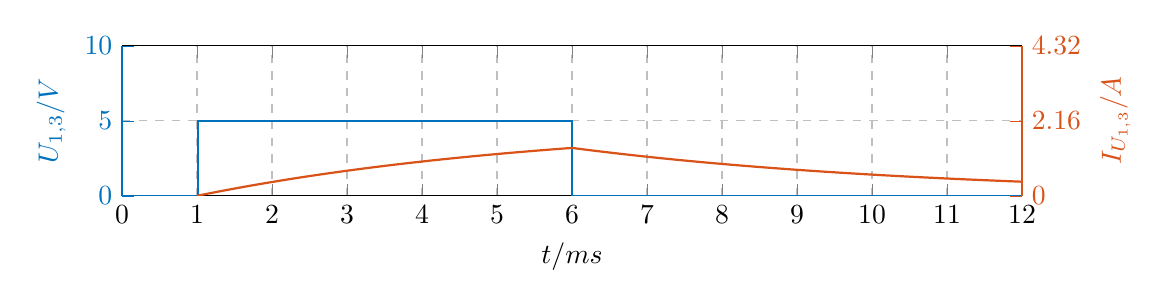
\begin{tikzpicture}
\pgfplotsset{
	width=4.5in,
	height=0.75in,
	every axis plot/.append style={thick}
}


\begin{axis}[%
scale only axis,
axis y line*=left,
ymin=0,
ymax=10,
xmin=0, xmax=12,
xlabel={$ t/ms $},
ytick={ 0, 5, 10},
ylabel style={font=\color{mycolor1}},
ylabel={$ U_{1,3}/V $},
ytick style={mycolor1},
yticklabel style={mycolor1},
y axis line style={mycolor1},
xmajorgrids,
ymajorgrids,
major grid style={dashed}
]
\addplot[const plot, color=mycolor1] table[row sep=crcr] {%
-1	0\\
-0.99	0\\
-0.98	0\\
-0.97	0\\
-0.96	0\\
-0.95	0\\
-0.94	0\\
-0.93	0\\
-0.92	0\\
-0.91	0\\
-0.9	0\\
-0.89	0\\
-0.88	0\\
-0.87	0\\
-0.86	0\\
-0.85	0\\
-0.84	0\\
-0.83	0\\
-0.82	0\\
-0.81	0\\
-0.8	0\\
-0.79	0\\
-0.78	0\\
-0.77	0\\
-0.76	0\\
-0.75	0\\
-0.74	0\\
-0.73	0\\
-0.72	0\\
-0.71	0\\
-0.7	0\\
-0.69	0\\
-0.68	0\\
-0.67	0\\
-0.66	0\\
-0.65	0\\
-0.64	0\\
-0.63	0\\
-0.62	0\\
-0.61	0\\
-0.6	0\\
-0.59	0\\
-0.58	0\\
-0.57	0\\
-0.56	0\\
-0.55	0\\
-0.54	0\\
-0.53	0\\
-0.52	0\\
-0.51	0\\
-0.5	0\\
-0.49	0\\
-0.48	0\\
-0.47	0\\
-0.46	0\\
-0.45	0\\
-0.44	0\\
-0.43	0\\
-0.42	0\\
-0.41	0\\
-0.4	0\\
-0.39	0\\
-0.38	0\\
-0.37	0\\
-0.36	0\\
-0.35	0\\
-0.34	0\\
-0.33	0\\
-0.32	0\\
-0.31	0\\
-0.3	0\\
-0.29	0\\
-0.28	0\\
-0.27	0\\
-0.26	0\\
-0.25	0\\
-0.24	0\\
-0.23	0\\
-0.22	0\\
-0.21	0\\
-0.2	0\\
-0.19	0\\
-0.18	0\\
-0.17	0\\
-0.16	0\\
-0.15	0\\
-0.14	0\\
-0.13	0\\
-0.12	0\\
-0.11	0\\
-0.1	0\\
-0.09	0\\
-0.08	0\\
-0.07	0\\
-0.0599999999999999	0\\
-0.0499999999999999	0\\
-0.04	0\\
-0.03	0\\
-0.02	0\\
-0.01	0\\
0	0\\
0.01	0\\
0.02	0\\
0.03	0\\
0.04	0\\
0.05	0\\
0.0600000000000001	0\\
0.0700000000000001	0\\
0.0800000000000001	0\\
0.0900000000000001	0\\
0.1	0\\
0.11	0\\
0.12	0\\
0.13	0\\
0.14	0\\
0.15	0\\
0.16	0\\
0.17	0\\
0.18	0\\
0.19	0\\
0.2	0\\
0.21	0\\
0.22	0\\
0.23	0\\
0.24	0\\
0.25	0\\
0.26	0\\
0.27	0\\
0.28	0\\
0.29	0\\
0.3	0\\
0.31	0\\
0.32	0\\
0.33	0\\
0.34	0\\
0.35	0\\
0.36	0\\
0.37	0\\
0.38	0\\
0.39	0\\
0.4	0\\
0.41	0\\
0.42	0\\
0.43	0\\
0.44	0\\
0.45	0\\
0.46	0\\
0.47	0\\
0.48	0\\
0.49	0\\
0.5	0\\
0.51	0\\
0.52	0\\
0.53	0\\
0.54	0\\
0.55	0\\
0.56	0\\
0.57	0\\
0.58	0\\
0.59	0\\
0.6	0\\
0.61	0\\
0.62	0\\
0.63	0\\
0.64	0\\
0.65	0\\
0.66	0\\
0.67	0\\
0.68	0\\
0.69	0\\
0.7	0\\
0.71	0\\
0.72	0\\
0.73	0\\
0.74	0\\
0.75	0\\
0.76	0\\
0.77	0\\
0.78	0\\
0.79	0\\
0.8	0\\
0.81	0\\
0.82	0\\
0.83	0\\
0.84	0\\
0.85	0\\
0.86	0\\
0.87	0\\
0.88	0\\
0.89	0\\
0.9	0\\
0.91	0\\
0.92	0\\
0.93	0\\
0.94	0\\
0.95	0\\
0.96	0\\
0.97	0\\
0.98	0\\
0.99	0\\
1	0\\
1.01	5\\
1.02	5\\
1.03	5\\
1.04	5\\
1.05	5\\
1.06	5\\
1.07	5\\
1.08	5\\
1.09	5\\
1.1	5\\
1.11	5\\
1.12	5\\
1.13	5\\
1.14	5\\
1.15	5\\
1.16	5\\
1.17	5\\
1.18	5\\
1.19	5\\
1.2	5\\
1.21	5\\
1.22	5\\
1.23	5\\
1.24	5\\
1.25	5\\
1.26	5\\
1.27	5\\
1.28	5\\
1.29	5\\
1.3	5\\
1.31	5\\
1.32	5\\
1.33	5\\
1.34	5\\
1.35	5\\
1.36	5\\
1.37	5\\
1.38	5\\
1.39	5\\
1.4	5\\
1.41	5\\
1.42	5\\
1.43	5\\
1.44	5\\
1.45	5\\
1.46	5\\
1.47	5\\
1.48	5\\
1.49	5\\
1.5	5\\
1.51	5\\
1.52	5\\
1.53	5\\
1.54	5\\
1.55	5\\
1.56	5\\
1.57	5\\
1.58	5\\
1.59	5\\
1.6	5\\
1.61	5\\
1.62	5\\
1.63	5\\
1.64	5\\
1.65	5\\
1.66	5\\
1.67	5\\
1.68	5\\
1.69	5\\
1.7	5\\
1.71	5\\
1.72	5\\
1.73	5\\
1.74	5\\
1.75	5\\
1.76	5\\
1.77	5\\
1.78	5\\
1.79	5\\
1.8	5\\
1.81	5\\
1.82	5\\
1.83	5\\
1.84	5\\
1.85	5\\
1.86	5\\
1.87	5\\
1.88	5\\
1.89	5\\
1.9	5\\
1.91	5\\
1.92	5\\
1.93	5\\
1.94	5\\
1.95	5\\
1.96	5\\
1.97	5\\
1.98	5\\
1.99	5\\
2	5\\
2.01	5\\
2.02	5\\
2.03	5\\
2.04	5\\
2.05	5\\
2.06	5\\
2.07	5\\
2.08	5\\
2.09	5\\
2.1	5\\
2.11	5\\
2.12	5\\
2.13	5\\
2.14	5\\
2.15	5\\
2.16	5\\
2.17	5\\
2.18	5\\
2.19	5\\
2.2	5\\
2.21	5\\
2.22	5\\
2.23	5\\
2.24	5\\
2.25	5\\
2.26	5\\
2.27	5\\
2.28	5\\
2.29	5\\
2.3	5\\
2.31	5\\
2.32	5\\
2.33	5\\
2.34	5\\
2.35	5\\
2.36	5\\
2.37	5\\
2.38	5\\
2.39	5\\
2.4	5\\
2.41	5\\
2.42	5\\
2.43	5\\
2.44	5\\
2.45	5\\
2.46	5\\
2.47	5\\
2.48	5\\
2.49	5\\
2.5	5\\
2.51	5\\
2.52	5\\
2.53	5\\
2.54	5\\
2.55	5\\
2.56	5\\
2.57	5\\
2.58	5\\
2.59	5\\
2.6	5\\
2.61	5\\
2.62	5\\
2.63	5\\
2.64	5\\
2.65	5\\
2.66	5\\
2.67	5\\
2.68	5\\
2.69	5\\
2.7	5\\
2.71	5\\
2.72	5\\
2.73	5\\
2.74	5\\
2.75	5\\
2.76	5\\
2.77	5\\
2.78	5\\
2.79	5\\
2.8	5\\
2.81	5\\
2.82	5\\
2.83	5\\
2.84	5\\
2.85	5\\
2.86	5\\
2.87	5\\
2.88	5\\
2.89	5\\
2.9	5\\
2.91	5\\
2.92	5\\
2.93	5\\
2.94	5\\
2.95	5\\
2.96	5\\
2.97	5\\
2.98	5\\
2.99	5\\
3	5\\
3.01	5\\
3.02	5\\
3.03	5\\
3.04	5\\
3.05	5\\
3.06	5\\
3.07	5\\
3.08	5\\
3.09	5\\
3.1	5\\
3.11	5\\
3.12	5\\
3.13	5\\
3.14	5\\
3.15	5\\
3.16	5\\
3.17	5\\
3.18	5\\
3.19	5\\
3.2	5\\
3.21	5\\
3.22	5\\
3.23	5\\
3.24	5\\
3.25	5\\
3.26	5\\
3.27	5\\
3.28	5\\
3.29	5\\
3.3	5\\
3.31	5\\
3.32	5\\
3.33	5\\
3.34	5\\
3.35	5\\
3.36	5\\
3.37	5\\
3.38	5\\
3.39	5\\
3.4	5\\
3.41	5\\
3.42	5\\
3.43	5\\
3.44	5\\
3.45	5\\
3.46	5\\
3.47	5\\
3.48	5\\
3.49	5\\
3.5	5\\
3.51	5\\
3.52	5\\
3.53	5\\
3.54	5\\
3.55	5\\
3.56	5\\
3.57	5\\
3.58	5\\
3.59	5\\
3.6	5\\
3.61	5\\
3.62	5\\
3.63	5\\
3.64	5\\
3.65	5\\
3.66	5\\
3.67	5\\
3.68	5\\
3.69	5\\
3.7	5\\
3.71	5\\
3.72	5\\
3.73	5\\
3.74	5\\
3.75	5\\
3.76	5\\
3.77	5\\
3.78	5\\
3.79	5\\
3.8	5\\
3.81	5\\
3.82	5\\
3.83	5\\
3.84	5\\
3.85	5\\
3.86	5\\
3.87	5\\
3.88	5\\
3.89	5\\
3.9	5\\
3.91	5\\
3.92	5\\
3.93	5\\
3.94	5\\
3.95	5\\
3.96	5\\
3.97	5\\
3.98	5\\
3.99	5\\
4	5\\
4.01	5\\
4.02	5\\
4.03	5\\
4.04	5\\
4.05	5\\
4.06	5\\
4.07	5\\
4.08	5\\
4.09	5\\
4.1	5\\
4.11	5\\
4.12	5\\
4.13	5\\
4.14	5\\
4.15	5\\
4.16	5\\
4.17	5\\
4.18	5\\
4.19	5\\
4.2	5\\
4.21	5\\
4.22	5\\
4.23	5\\
4.24	5\\
4.25	5\\
4.26	5\\
4.27	5\\
4.28	5\\
4.29	5\\
4.3	5\\
4.31	5\\
4.32	5\\
4.33	5\\
4.34	5\\
4.35	5\\
4.36	5\\
4.37	5\\
4.38	5\\
4.39	5\\
4.4	5\\
4.41	5\\
4.42	5\\
4.43	5\\
4.44	5\\
4.45	5\\
4.46	5\\
4.47	5\\
4.48	5\\
4.49	5\\
4.5	5\\
4.51	5\\
4.52	5\\
4.53	5\\
4.54	5\\
4.55	5\\
4.56	5\\
4.57	5\\
4.58	5\\
4.59	5\\
4.6	5\\
4.61	5\\
4.62	5\\
4.63	5\\
4.64	5\\
4.65	5\\
4.66	5\\
4.67	5\\
4.68	5\\
4.69	5\\
4.7	5\\
4.71	5\\
4.72	5\\
4.73	5\\
4.74	5\\
4.75	5\\
4.76	5\\
4.77	5\\
4.78	5\\
4.79	5\\
4.8	5\\
4.81	5\\
4.82	5\\
4.83	5\\
4.84	5\\
4.85	5\\
4.86	5\\
4.87	5\\
4.88	5\\
4.89	5\\
4.9	5\\
4.91	5\\
4.92	5\\
4.93	5\\
4.94	5\\
4.95	5\\
4.96	5\\
4.97	5\\
4.98	5\\
4.99	5\\
5	5\\
5.01	5\\
5.02	5\\
5.03	5\\
5.04	5\\
5.05	5\\
5.06	5\\
5.07	5\\
5.08	5\\
5.09	5\\
5.1	5\\
5.11	5\\
5.12	5\\
5.13	5\\
5.14	5\\
5.15	5\\
5.16	5\\
5.17	5\\
5.18	5\\
5.19	5\\
5.2	5\\
5.21	5\\
5.22	5\\
5.23	5\\
5.24	5\\
5.25	5\\
5.26	5\\
5.27	5\\
5.28	5\\
5.29	5\\
5.3	5\\
5.31	5\\
5.32	5\\
5.33	5\\
5.34	5\\
5.35	5\\
5.36	5\\
5.37	5\\
5.38	5\\
5.39	5\\
5.4	5\\
5.41	5\\
5.42	5\\
5.43	5\\
5.44	5\\
5.45	5\\
5.46	5\\
5.47	5\\
5.48	5\\
5.49	5\\
5.5	5\\
5.51	5\\
5.52	5\\
5.53	5\\
5.54	5\\
5.55	5\\
5.56	5\\
5.57	5\\
5.58	5\\
5.59	5\\
5.6	5\\
5.61	5\\
5.62	5\\
5.63	5\\
5.64	5\\
5.65	5\\
5.66	5\\
5.67	5\\
5.68	5\\
5.69	5\\
5.7	5\\
5.71	5\\
5.72	5\\
5.73	5\\
5.74	5\\
5.75	5\\
5.76	5\\
5.77	5\\
5.78	5\\
5.79	5\\
5.8	5\\
5.81	5\\
5.82	5\\
5.83	5\\
5.84	5\\
5.85	5\\
5.86	5\\
5.87	5\\
5.88	5\\
5.89	5\\
5.9	5\\
5.91	5\\
5.92	5\\
5.93	5\\
5.94	5\\
5.95	5\\
5.96	5\\
5.97	5\\
5.98	5\\
5.99	5\\
6	0\\
6.01	0\\
6.02	0\\
6.03	0\\
6.04	0\\
6.05	0\\
6.06	0\\
6.07	0\\
6.08	0\\
6.09	0\\
6.1	0\\
6.11	0\\
6.12	0\\
6.13	0\\
6.14	0\\
6.15	0\\
6.16	0\\
6.17	0\\
6.18	0\\
6.19	0\\
6.2	0\\
6.21	0\\
6.22	0\\
6.23	0\\
6.24	0\\
6.25	0\\
6.26	0\\
6.27	0\\
6.28	0\\
6.29	0\\
6.3	0\\
6.31	0\\
6.32	0\\
6.33	0\\
6.34	0\\
6.35	0\\
6.36	0\\
6.37	0\\
6.38	0\\
6.39	0\\
6.4	0\\
6.41	0\\
6.42	0\\
6.43	0\\
6.44	0\\
6.45	0\\
6.46	0\\
6.47	0\\
6.48	0\\
6.49	0\\
6.5	0\\
6.51	0\\
6.52	0\\
6.53	0\\
6.54	0\\
6.55	0\\
6.56	0\\
6.57	0\\
6.58	0\\
6.59	0\\
6.6	0\\
6.61	0\\
6.62	0\\
6.63	0\\
6.64	0\\
6.65	0\\
6.66	0\\
6.67	0\\
6.68	0\\
6.69	0\\
6.7	0\\
6.71	0\\
6.72	0\\
6.73	0\\
6.74	0\\
6.75	0\\
6.76	0\\
6.77	0\\
6.78	0\\
6.79	0\\
6.8	0\\
6.81	0\\
6.82	0\\
6.83	0\\
6.84	0\\
6.85	0\\
6.86	0\\
6.87	0\\
6.88	0\\
6.89	0\\
6.9	0\\
6.91	0\\
6.92	0\\
6.93	0\\
6.94	0\\
6.95	0\\
6.96	0\\
6.97	0\\
6.98	0\\
6.99	0\\
7	0\\
7.01	0\\
7.02	0\\
7.03	0\\
7.04	0\\
7.05	0\\
7.06	0\\
7.07	0\\
7.08	0\\
7.09	0\\
7.1	0\\
7.11	0\\
7.12	0\\
7.13	0\\
7.14	0\\
7.15	0\\
7.16	0\\
7.17	0\\
7.18	0\\
7.19	0\\
7.2	0\\
7.21	0\\
7.22	0\\
7.23	0\\
7.24	0\\
7.25	0\\
7.26	0\\
7.27	0\\
7.28	0\\
7.29	0\\
7.3	0\\
7.31	0\\
7.32	0\\
7.33	0\\
7.34	0\\
7.35	0\\
7.36	0\\
7.37	0\\
7.38	0\\
7.39	0\\
7.4	0\\
7.41	0\\
7.42	0\\
7.43	0\\
7.44	0\\
7.45	0\\
7.46	0\\
7.47	0\\
7.48	0\\
7.49	0\\
7.5	0\\
7.51	0\\
7.52	0\\
7.53	0\\
7.54	0\\
7.55	0\\
7.56	0\\
7.57	0\\
7.58	0\\
7.59	0\\
7.6	0\\
7.61	0\\
7.62	0\\
7.63	0\\
7.64	0\\
7.65	0\\
7.66	0\\
7.67	0\\
7.68	0\\
7.69	0\\
7.7	0\\
7.71	0\\
7.72	0\\
7.73	0\\
7.74	0\\
7.75	0\\
7.76	0\\
7.77	0\\
7.78	0\\
7.79	0\\
7.8	0\\
7.81	0\\
7.82	0\\
7.83	0\\
7.84	0\\
7.85	0\\
7.86	0\\
7.87	0\\
7.88	0\\
7.89	0\\
7.9	0\\
7.91	0\\
7.92	0\\
7.93	0\\
7.94	0\\
7.95	0\\
7.96	0\\
7.97	0\\
7.98	0\\
7.99	0\\
8	0\\
8.01	0\\
8.02	0\\
8.03	0\\
8.04	0\\
8.05	0\\
8.06	0\\
8.07	0\\
8.08	0\\
8.09	0\\
8.1	0\\
8.11	0\\
8.12	0\\
8.13	0\\
8.14	0\\
8.15	0\\
8.16	0\\
8.17	0\\
8.18	0\\
8.19	0\\
8.2	0\\
8.21	0\\
8.22	0\\
8.23	0\\
8.24	0\\
8.25	0\\
8.26	0\\
8.27	0\\
8.28	0\\
8.29	0\\
8.3	0\\
8.31	0\\
8.32	0\\
8.33	0\\
8.34	0\\
8.35	0\\
8.36	0\\
8.37	0\\
8.38	0\\
8.39	0\\
8.4	0\\
8.41	0\\
8.42	0\\
8.43	0\\
8.44	0\\
8.45	0\\
8.46	0\\
8.47	0\\
8.48	0\\
8.49	0\\
8.5	0\\
8.51	0\\
8.52	0\\
8.53	0\\
8.54	0\\
8.55	0\\
8.56	0\\
8.57	0\\
8.58	0\\
8.59	0\\
8.6	0\\
8.61	0\\
8.62	0\\
8.63	0\\
8.64	0\\
8.65	0\\
8.66	0\\
8.67	0\\
8.68	0\\
8.69	0\\
8.7	0\\
8.71	0\\
8.72	0\\
8.73	0\\
8.74	0\\
8.75	0\\
8.76	0\\
8.77	0\\
8.78	0\\
8.79	0\\
8.8	0\\
8.81	0\\
8.82	0\\
8.83	0\\
8.84	0\\
8.85	0\\
8.86	0\\
8.87	0\\
8.88	0\\
8.89	0\\
8.9	0\\
8.91	0\\
8.92	0\\
8.93	0\\
8.94	0\\
8.95	0\\
8.96	0\\
8.97	0\\
8.98	0\\
8.99	0\\
9	0\\
9.01	0\\
9.02	0\\
9.03	0\\
9.04	0\\
9.05	0\\
9.06	0\\
9.07	0\\
9.08	0\\
9.09	0\\
9.1	0\\
9.11	0\\
9.12	0\\
9.13	0\\
9.14	0\\
9.15	0\\
9.16	0\\
9.17	0\\
9.18	0\\
9.19	0\\
9.2	0\\
9.21	0\\
9.22	0\\
9.23	0\\
9.24	0\\
9.25	0\\
9.26	0\\
9.27	0\\
9.28	0\\
9.29	0\\
9.3	0\\
9.31	0\\
9.32	0\\
9.33	0\\
9.34	0\\
9.35	0\\
9.36	0\\
9.37	0\\
9.38	0\\
9.39	0\\
9.4	0\\
9.41	0\\
9.42	0\\
9.43	0\\
9.44	0\\
9.45	0\\
9.46	0\\
9.47	0\\
9.48	0\\
9.49	0\\
9.5	0\\
9.51	0\\
9.52	0\\
9.53	0\\
9.54	0\\
9.55	0\\
9.56	0\\
9.57	0\\
9.58	0\\
9.59	0\\
9.6	0\\
9.61	0\\
9.62	0\\
9.63	0\\
9.64	0\\
9.65	0\\
9.66	0\\
9.67	0\\
9.68	0\\
9.69	0\\
9.7	0\\
9.71	0\\
9.72	0\\
9.73	0\\
9.74	0\\
9.75	0\\
9.76	0\\
9.77	0\\
9.78	0\\
9.79	0\\
9.8	0\\
9.81	0\\
9.82	0\\
9.83	0\\
9.84	0\\
9.85	0\\
9.86	0\\
9.87	0\\
9.88	0\\
9.89	0\\
9.9	0\\
9.91	0\\
9.92	0\\
9.93	0\\
9.94	0\\
9.95	0\\
9.96	0\\
9.97	0\\
9.98	0\\
9.99	0\\
10	0\\
10.01	0\\
10.02	0\\
10.03	0\\
10.04	0\\
10.05	0\\
10.06	0\\
10.07	0\\
10.08	0\\
10.09	0\\
10.1	0\\
10.11	0\\
10.12	0\\
10.13	0\\
10.14	0\\
10.15	0\\
10.16	0\\
10.17	0\\
10.18	0\\
10.19	0\\
10.2	0\\
10.21	0\\
10.22	0\\
10.23	0\\
10.24	0\\
10.25	0\\
10.26	0\\
10.27	0\\
10.28	0\\
10.29	0\\
10.3	0\\
10.31	0\\
10.32	0\\
10.33	0\\
10.34	0\\
10.35	0\\
10.36	0\\
10.37	0\\
10.38	0\\
10.39	0\\
10.4	0\\
10.41	0\\
10.42	0\\
10.43	0\\
10.44	0\\
10.45	0\\
10.46	0\\
10.47	0\\
10.48	0\\
10.49	0\\
10.5	0\\
10.51	0\\
10.52	0\\
10.53	0\\
10.54	0\\
10.55	0\\
10.56	0\\
10.57	0\\
10.58	0\\
10.59	0\\
10.6	0\\
10.61	0\\
10.62	0\\
10.63	0\\
10.64	0\\
10.65	0\\
10.66	0\\
10.67	0\\
10.68	0\\
10.69	0\\
10.7	0\\
10.71	0\\
10.72	0\\
10.73	0\\
10.74	0\\
10.75	0\\
10.76	0\\
10.77	0\\
10.78	0\\
10.79	0\\
10.8	0\\
10.81	0\\
10.82	0\\
10.83	0\\
10.84	0\\
10.85	0\\
10.86	0\\
10.87	0\\
10.88	0\\
10.89	0\\
10.9	0\\
10.91	0\\
10.92	0\\
10.93	0\\
10.94	0\\
10.95	0\\
10.96	0\\
10.97	0\\
10.98	0\\
10.99	0\\
11	0\\
11.01	0\\
11.02	0\\
11.03	0\\
11.04	0\\
11.05	0\\
11.06	0\\
11.07	0\\
11.08	0\\
11.09	0\\
11.1	0\\
11.11	0\\
11.12	0\\
11.13	0\\
11.14	0\\
11.15	0\\
11.16	0\\
11.17	0\\
11.18	0\\
11.19	0\\
11.2	0\\
11.21	0\\
11.22	0\\
11.23	0\\
11.24	0\\
11.25	0\\
11.26	0\\
11.27	0\\
11.28	0\\
11.29	0\\
11.3	0\\
11.31	0\\
11.32	0\\
11.33	0\\
11.34	0\\
11.35	0\\
11.36	0\\
11.37	0\\
11.38	0\\
11.39	0\\
11.4	0\\
11.41	0\\
11.42	0\\
11.43	0\\
11.44	0\\
11.45	0\\
11.46	0\\
11.47	0\\
11.48	0\\
11.49	0\\
11.5	0\\
11.51	0\\
11.52	0\\
11.53	0\\
11.54	0\\
11.55	0\\
11.56	0\\
11.57	0\\
11.58	0\\
11.59	0\\
11.6	0\\
11.61	0\\
11.62	0\\
11.63	0\\
11.64	0\\
11.65	0\\
11.66	0\\
11.67	0\\
11.68	0\\
11.69	0\\
11.7	0\\
11.71	0\\
11.72	0\\
11.73	0\\
11.74	0\\
11.75	0\\
11.76	0\\
11.77	0\\
11.78	0\\
11.79	0\\
11.8	0\\
11.81	0\\
11.82	0\\
11.83	0\\
11.84	0\\
11.85	0\\
11.86	0\\
11.87	0\\
11.88	0\\
11.89	0\\
11.9	0\\
11.91	0\\
11.92	0\\
11.93	0\\
11.94	0\\
11.95	0\\
11.96	0\\
11.97	0\\
11.98	0\\
11.99	0\\
12	0\\
};
\end{axis}

\begin{axis}[
scale only axis,
axis y line*=right,
axis x line=none,
xmin=0,
xmax=12,
ymin=0,
ymax=4.32,
ytick={   0, 2.16, 4.32},
ytick style={mycolor2},
ylabel style={font=\color{mycolor2}},
yticklabel style={mycolor2},
y axis line style={mycolor2},
ylabel={$ I_{U_{1,3}}/A $}
]

\addplot [color=mycolor2]
  table[row sep=crcr]{%
-1	-3.24605430007372\\
-0.99	-3.23944991924123\\
-0.98	-3.23285897559807\\
-0.97	-3.22628144180509\\
-0.96	-3.21971729057879\\
-0.95	-3.21316649469117\\
-0.94	-3.20662902696962\\
-0.93	-3.20010486029683\\
-0.92	-3.19359396761065\\
-0.91	-3.18709632190399\\
-0.9	-3.18061189622473\\
-0.89	-3.17414066367557\\
-0.88	-3.16768259741391\\
-0.87	-3.16123767065182\\
-0.86	-3.15480585665582\\
-0.85	-3.14838712874685\\
-0.84	-3.14198146030012\\
-0.83	-3.13558882474502\\
-0.82	-3.12920919556499\\
-0.81	-3.12284254629743\\
-0.8	-3.11648885053357\\
-0.79	-3.11014808191837\\
-0.78	-3.10382021415043\\
-0.77	-3.09750522098185\\
-0.76	-3.09120307621812\\
-0.75	-3.08491375371805\\
-0.74	-3.07863722739363\\
-0.73	-3.07237347120991\\
-0.72	-3.06612245918493\\
-0.71	-3.05988416538958\\
-0.7	-3.05365856394753\\
-0.69	-3.04744562903506\\
-0.68	-3.04124533488102\\
-0.67	-3.03505765576668\\
-0.66	-3.02888256602564\\
-0.65	-3.02272004004373\\
-0.64	-3.01657005225887\\
-0.63	-3.01043257716101\\
-0.62	-3.004307589292\\
-0.61	-2.99819506324548\\
-0.6	-2.99209497366679\\
-0.59	-2.98600729525284\\
-0.58	-2.97993200275204\\
-0.57	-2.97386907096416\\
-0.56	-2.96781847474026\\
-0.55	-2.96178018898256\\
-0.54	-2.95575418864433\\
-0.53	-2.94974044872981\\
-0.52	-2.94373894429412\\
-0.51	-2.93774965044309\\
-0.5	-2.93177254233322\\
-0.49	-2.92580759517157\\
-0.48	-2.91985478421562\\
-0.47	-2.9139140847732\\
-0.46	-2.90798547220237\\
-0.45	-2.90206892191135\\
-0.44	-2.89616440935838\\
-0.43	-2.89027191005162\\
-0.42	-2.88439139954907\\
-0.41	-2.87852285345847\\
-0.4	-2.87266624743718\\
-0.39	-2.86682155719208\\
-0.38	-2.86098875847948\\
-0.37	-2.85516782710503\\
-0.36	-2.84935873892359\\
-0.35	-2.84356146983916\\
-0.34	-2.83777599580473\\
-0.33	-2.83200229282227\\
-0.32	-2.82624033694252\\
-0.31	-2.820490104265\\
-0.3	-2.81475157093781\\
-0.29	-2.80902471315762\\
-0.28	-2.80330950716949\\
-0.27	-2.79760592926685\\
-0.26	-2.79191395579134\\
-0.25	-2.78623356313273\\
-0.24	-2.78056472772884\\
-0.23	-2.77490742606544\\
-0.22	-2.76926163467612\\
-0.21	-2.76362733014222\\
-0.2	-2.75800448909273\\
-0.19	-2.75239308820419\\
-0.18	-2.7467931042006\\
-0.17	-2.7412045138533\\
-0.16	-2.73562729398091\\
-0.15	-2.73006142144921\\
-0.14	-2.72450687317104\\
-0.13	-2.71896362610621\\
-0.12	-2.71343165726143\\
-0.11	-2.70791094369016\\
-0.1	-2.70240146249258\\
-0.09	-2.69690319081543\\
-0.08	-2.69141610585198\\
-0.07	-2.68594018484187\\
-0.0599999999999999	-2.68047540507106\\
-0.0499999999999999	-2.67502174387174\\
-0.04	-2.6695791786222\\
-0.03	-2.66414768674675\\
-0.02	-2.65872724571566\\
-0.01	-2.65331783304502\\
0	-2.64791942629666\\
0.01	-2.64253200307808\\
0.02	-2.63715554104232\\
0.03	-2.6317900178879\\
0.04	-2.62643541135871\\
0.05	-2.62109169924393\\
0.0600000000000001	-2.61575885937792\\
0.0700000000000001	-2.61043686964013\\
0.0800000000000001	-2.60512570795504\\
0.0900000000000001	-2.59982535229203\\
0.1	-2.5945357806653\\
0.11	-2.58925697113379\\
0.12	-2.58398890180108\\
0.13	-2.57873155081529\\
0.14	-2.57348489636902\\
0.15	-2.56824891669921\\
0.16	-2.56302359008711\\
0.17	-2.55780889485813\\
0.18	-2.55260480938181\\
0.19	-2.54741131207167\\
0.2	-2.54222838138517\\
0.21	-2.53705599582358\\
0.22	-2.53189413393194\\
0.23	-2.52674277429891\\
0.24	-2.52160189555673\\
0.25	-2.51647147638112\\
0.26	-2.51135149549117\\
0.27	-2.50624193164928\\
0.28	-2.50114276366106\\
0.29	-2.49605397037524\\
0.3	-2.49097553068357\\
0.31	-2.48590742352077\\
0.32	-2.48084962786441\\
0.33	-2.47580212273482\\
0.34	-2.47076488719503\\
0.35	-2.46573790035066\\
0.36	-2.46072114134985\\
0.37	-2.45571458938316\\
0.38	-2.45071822368348\\
0.39	-2.44573202352597\\
0.4	-2.44075596822794\\
0.41	-2.43579003714879\\
0.42	-2.43083420968991\\
0.43	-2.42588846529461\\
0.44	-2.42095278344801\\
0.45	-2.41602714367698\\
0.46	-2.41111152555005\\
0.47	-2.40620590867729\\
0.48	-2.40131027271029\\
0.49	-2.39642459734201\\
0.5	-2.39154886230677\\
0.51	-2.38668304738007\\
0.52	-2.38182713237859\\
0.53	-2.37698109716007\\
0.54	-2.37214492162323\\
0.55	-2.36731858570769\\
0.56	-2.36250206939387\\
0.57	-2.35769535270295\\
0.58	-2.35289841569672\\
0.59	-2.34811123847758\\
0.6	-2.34333380118838\\
0.61	-2.33856608401238\\
0.62	-2.33380806717316\\
0.63	-2.32905973093455\\
0.64	-2.32432105560052\\
0.65	-2.3195920215151\\
0.66	-2.31487260906235\\
0.67	-2.3101627986662\\
0.68	-2.30546257079044\\
0.69	-2.30077190593859\\
0.7	-2.29609078465385\\
0.71	-2.29141918751899\\
0.72	-2.28675709515631\\
0.73	-2.2821044882275\\
0.74	-2.27746134743363\\
0.75	-2.27282765351503\\
0.76	-2.26820338725119\\
0.77	-2.26358852946073\\
0.78	-2.25898306100129\\
0.79	-2.25438696276946\\
0.8	-2.2498002157007\\
0.81	-2.24522280076923\\
0.82	-2.24065469898802\\
0.83	-2.23609589140866\\
0.84	-2.23154635912126\\
0.85	-2.22700608325445\\
0.86	-2.22247504497522\\
0.87	-2.21795322548891\\
0.88	-2.21344060603906\\
0.89	-2.20893716790741\\
0.9	-2.20444289241375\\
0.91	-2.19995776091591\\
0.92	-2.19548175480962\\
0.93	-2.19101485552848\\
0.94	-2.18655704454386\\
0.95	-2.18210830336482\\
0.96	-2.17766861353806\\
0.97	-2.17323795664781\\
0.98	-2.16881631431576\\
0.99	-2.16440366820102\\
1	-1.08\\
1.01	0.00439470855365792\\
1.02	0.00878047568913453\\
1.03	0.0131573195985256\\
1.04	0.0175252584369137\\
1.05	0.0218843103224427\\
1.06	0.0262344933363947\\
1.07	0.0305758255232624\\
1.08	0.0349083248908268\\
1.09	0.0392320094102293\\
1.1	0.0435468970160482\\
1.11	0.0478530056063718\\
1.12	0.052150353042874\\
1.13	0.0564389571508863\\
1.14	0.0607188357194746\\
1.15	0.06499000650151\\
1.16	0.0692524872137446\\
1.17	0.0735062955368837\\
1.18	0.0777514491156602\\
1.19	0.0819879655589069\\
1.2	0.0862158624396304\\
1.21	0.0904351572950825\\
1.22	0.0946458676268348\\
1.23	0.0988480109008499\\
1.24	0.103041604547555\\
1.25	0.107226665961913\\
1.26	0.111403212503495\\
1.27	0.115571261496554\\
1.28	0.119730830230094\\
1.29	0.123881935957942\\
1.3	0.128024595898823\\
1.31	0.132158827236427\\
1.32	0.136284647119484\\
1.33	0.140402072661833\\
1.34	0.144511120942492\\
1.35	0.148611809005731\\
1.36	0.152704153861142\\
1.37	0.156788172483711\\
1.38	0.160863881813884\\
1.39	0.164931298757643\\
1.4	0.168990440186571\\
1.41	0.173041322937926\\
1.42	0.177083963814708\\
1.43	0.181118379585731\\
1.44	0.18514458698569\\
1.45	0.189162602715232\\
1.46	0.193172443441026\\
1.47	0.197174125795832\\
1.48	0.201167666378566\\
1.49	0.205153081754375\\
1.5	0.209130388454702\\
1.51	0.213099602977354\\
1.52	0.217060741786575\\
1.53	0.221013821313106\\
1.54	0.224958857954263\\
1.55	0.228895868073999\\
1.56	0.232824868002971\\
1.57	0.236745874038611\\
1.58	0.240658902445195\\
1.59	0.244563969453904\\
1.6	0.248461091262897\\
1.61	0.252350284037377\\
1.62	0.256231563909656\\
1.63	0.260104946979226\\
1.64	0.26397044931282\\
1.65	0.267828086944483\\
1.66	0.271677875875639\\
1.67	0.275519832075153\\
1.68	0.279353971479402\\
1.69	0.283180309992338\\
1.7	0.286998863485556\\
1.71	0.290809647798357\\
1.72	0.294612678737818\\
1.73	0.298407972078853\\
1.74	0.302195543564282\\
1.75	0.305975408904894\\
1.76	0.309747583779513\\
1.77	0.313512083835064\\
1.78	0.317268924686637\\
1.79	0.321018121917549\\
1.8	0.324759691079415\\
1.81	0.328493647692207\\
1.82	0.332220007244321\\
1.83	0.335938785192639\\
1.84	0.339649996962597\\
1.85	0.343353657948245\\
1.86	0.347049783512313\\
1.87	0.350738388986273\\
1.88	0.354419489670406\\
1.89	0.358093100833861\\
1.9	0.361759237714723\\
1.91	0.36541791552007\\
1.92	0.369069149426045\\
1.93	0.37271295457791\\
1.94	0.376349346090112\\
1.95	0.379978339046351\\
1.96	0.383599948499633\\
1.97	0.38721418947234\\
1.98	0.390821076956289\\
1.99	0.394420625912794\\
2	0.39801285127273\\
2.01	0.401597767936595\\
2.02	0.405175390774567\\
2.03	0.408745734626573\\
2.04	0.412308814302344\\
2.05	0.415864644581482\\
2.06	0.419413240213517\\
2.07	0.422954615917969\\
2.08	0.426488786384412\\
2.09	0.430015766272532\\
2.1	0.433535570212187\\
2.11	0.437048212803472\\
2.12	0.440553708616774\\
2.13	0.444052072192837\\
2.14	0.447543318042821\\
2.15	0.451027460648361\\
2.16	0.454504514461627\\
2.17	0.457974493905387\\
2.18	0.461437413373062\\
2.19	0.46489328722879\\
2.2	0.468342129807484\\
2.21	0.47178395541489\\
2.22	0.475218778327649\\
2.23	0.478646612793356\\
2.24	0.482067473030614\\
2.25	0.485481373229102\\
2.26	0.488888327549625\\
2.27	0.492288350124178\\
2.28	0.495681455056004\\
2.29	0.499067656419651\\
2.3	0.50244696826103\\
2.31	0.505819404597477\\
2.32	0.509184979417806\\
2.33	0.51254370668237\\
2.34	0.51589560032312\\
2.35	0.519240674243661\\
2.36	0.522578942319306\\
2.37	0.525910418397144\\
2.38	0.529235116296085\\
2.39	0.532553049806927\\
2.4	0.535864232692408\\
2.41	0.539168678687263\\
2.42	0.542466401498286\\
2.43	0.545757414804381\\
2.44	0.549041732256621\\
2.45	0.552319367478305\\
2.46	0.555590334065015\\
2.47	0.55885464558467\\
2.48	0.562112315577586\\
2.49	0.565363357556529\\
2.5	0.56860778500677\\
2.51	0.571845611386148\\
2.52	0.575076850125116\\
2.53	0.578301514626804\\
2.54	0.581519618267071\\
2.55	0.584731174394563\\
2.56	0.587936196330766\\
2.57	0.591134697370063\\
2.58	0.594326690779787\\
2.59	0.59751218980028\\
2.6	0.600691207644942\\
2.61	0.603863757500292\\
2.62	0.607029852526019\\
2.63	0.610189505855038\\
2.64	0.613342730593541\\
2.65	0.616489539821058\\
2.66	0.619629946590507\\
2.67	0.622763963928246\\
2.68	0.625891604834133\\
2.69	0.629012882281575\\
2.7	0.632127809217583\\
2.71	0.635236398562827\\
2.72	0.638338663211689\\
2.73	0.641434616032316\\
2.74	0.644524269866673\\
2.75	0.647607637530598\\
2.76	0.650684731813853\\
2.77	0.653755565480179\\
2.78	0.656820151267348\\
2.79	0.659878501887214\\
2.8	0.662930630025771\\
2.81	0.665976548343199\\
2.82	0.669016269473922\\
2.83	0.672049806026657\\
2.84	0.675077170584468\\
2.85	0.678098375704817\\
2.86	0.681113433919618\\
2.87	0.684122357735286\\
2.88	0.687125159632792\\
2.89	0.690121852067713\\
2.9	0.693112447470284\\
2.91	0.696096958245449\\
2.92	0.699075396772914\\
2.93	0.702047775407197\\
2.94	0.705014106477679\\
2.95	0.707974402288658\\
2.96	0.710928675119395\\
2.97	0.71387693722417\\
2.98	0.716819200832329\\
2.99	0.719755478148336\\
3	0.722685781351827\\
3.01	0.725610122597654\\
3.02	0.728528514015942\\
3.03	0.731440967712132\\
3.04	0.73434749576704\\
3.05	0.7372481102369\\
3.06	0.740142823153416\\
3.07	0.743031646523814\\
3.08	0.74591459233089\\
3.09	0.748791672533059\\
3.1	0.751662899064407\\
3.11	0.754528283834739\\
3.12	0.757387838729626\\
3.13	0.760241575610459\\
3.14	0.763089506314496\\
3.15	0.76593164265491\\
3.16	0.768767996420839\\
3.17	0.771598579377437\\
3.18	0.774423403265919\\
3.19	0.777242479803611\\
3.2	0.780055820684001\\
3.21	0.782863437576784\\
3.22	0.785665342127912\\
3.23	0.788461545959643\\
3.24	0.791252060670588\\
3.25	0.79403689783576\\
3.26	0.796816069006622\\
3.27	0.799589585711134\\
3.28	0.802357459453801\\
3.29	0.805119701715722\\
3.3	0.807876323954635\\
3.31	0.810627337604968\\
3.32	0.813372754077885\\
3.33	0.81611258476133\\
3.34	0.818846841020081\\
3.35	0.821575534195792\\
3.36	0.824298675607039\\
3.37	0.827016276549373\\
3.38	0.829728348295362\\
3.39	0.832434902094637\\
3.4	0.835135949173944\\
3.41	0.837831500737184\\
3.42	0.840521567965466\\
3.43	0.843206162017146\\
3.44	0.845885294027881\\
3.45	0.848558975110669\\
3.46	0.8512272163559\\
3.47	0.853890028831398\\
3.48	0.856547423582468\\
3.49	0.859199411631945\\
3.5	0.861846003980234\\
3.51	0.86448721160536\\
3.52	0.867123045463014\\
3.53	0.869753516486593\\
3.54	0.872378635587252\\
3.55	0.874998413653945\\
3.56	0.877612861553472\\
3.57	0.880221990130524\\
3.58	0.882825810207726\\
3.59	0.885424332585685\\
3.6	0.888017568043032\\
3.61	0.890605527336469\\
3.62	0.893188221200812\\
3.63	0.895765660349036\\
3.64	0.898337855472319\\
3.65	0.900904817240089\\
3.66	0.903466556300063\\
3.67	0.906023083278297\\
3.68	0.908574408779225\\
3.69	0.911120543385709\\
3.7	0.913661497659075\\
3.71	0.916197282139163\\
3.72	0.91872790734437\\
3.73	0.921253383771689\\
3.74	0.92377372189676\\
3.75	0.926288932173907\\
3.76	0.928799025036184\\
3.77	0.931304010895418\\
3.78	0.933803900142252\\
3.79	0.936298703146191\\
3.8	0.938788430255638\\
3.81	0.941273091797944\\
3.82	0.943752698079448\\
3.83	0.946227259385519\\
3.84	0.9486967859806\\
3.85	0.951161288108251\\
3.86	0.953620775991187\\
3.87	0.956075259831329\\
3.88	0.958524749809838\\
3.89	0.960969256087162\\
3.9	0.963408788803075\\
3.91	0.965843358076723\\
3.92	0.968272974006661\\
3.93	0.970697646670901\\
3.94	0.973117386126948\\
3.95	0.975532202411844\\
3.96	0.977942105542211\\
3.97	0.980347105514291\\
3.98	0.982747212303987\\
3.99	0.985142435866906\\
4	0.987532786138399\\
4.01	0.989918273033603\\
4.02	0.992298906447482\\
4.03	0.994674696254867\\
4.04	0.997045652310498\\
4.05	0.999411784449065\\
4.06	1.00177310248525\\
4.07	1.00412961621376\\
4.08	1.00648133540938\\
4.09	1.00882826982701\\
4.1	1.0111704292017\\
4.11	1.01350782324868\\
4.12	1.01584046166344\\
4.13	1.01816835412171\\
4.14	1.02049151027957\\
4.15	1.02280993977343\\
4.16	1.02512365222011\\
4.17	1.02743265721683\\
4.18	1.02973696434133\\
4.19	1.03203658315184\\
4.2	1.03433152318713\\
4.21	1.03662179396659\\
4.22	1.03890740499023\\
4.23	1.04118836573871\\
4.24	1.04346468567345\\
4.25	1.04573637423656\\
4.26	1.04800344085099\\
4.27	1.0502658949205\\
4.28	1.0525237458297\\
4.29	1.05477700294414\\
4.3	1.05702567561027\\
4.31	1.05926977315558\\
4.32	1.06150930488854\\
4.33	1.06374428009868\\
4.34	1.06597470805667\\
4.35	1.06820059801427\\
4.36	1.07042195920445\\
4.37	1.07263880084138\\
4.38	1.07485113212048\\
4.39	1.07705896221847\\
4.4	1.0792623002934\\
4.41	1.08146115548468\\
4.42	1.08365553691312\\
4.43	1.085845453681\\
4.44	1.08803091487204\\
4.45	1.09021192955152\\
4.46	1.09238850676624\\
4.47	1.09456065554462\\
4.48	1.09672838489669\\
4.49	1.09889170381417\\
4.5	1.10105062127047\\
4.51	1.10320514622075\\
4.52	1.10535528760194\\
4.53	1.10750105433279\\
4.54	1.10964245531392\\
4.55	1.11177949942782\\
4.56	1.11391219553893\\
4.57	1.11604055249362\\
4.58	1.1181645791203\\
4.59	1.1202842842294\\
4.6	1.12239967661341\\
4.61	1.12451076504696\\
4.62	1.1266175582868\\
4.63	1.1287200650719\\
4.64	1.1308182941234\\
4.65	1.13291225414473\\
4.66	1.13500195382162\\
4.67	1.13708740182209\\
4.68	1.13916860679656\\
4.69	1.14124557737784\\
4.7	1.14331832218116\\
4.71	1.14538684980424\\
4.72	1.1474511688273\\
4.73	1.14951128781311\\
4.74	1.15156721530701\\
4.75	1.15361895983696\\
4.76	1.15566652991355\\
4.77	1.15770993403009\\
4.78	1.15974918066257\\
4.79	1.16178427826977\\
4.8	1.16381523529323\\
4.81	1.16584206015734\\
4.82	1.16786476126934\\
4.83	1.16988334701936\\
4.84	1.17189782578045\\
4.85	1.17390820590866\\
4.86	1.17591449574301\\
4.87	1.17791670360555\\
4.88	1.17991483780141\\
4.89	1.18190890661883\\
4.9	1.18389891832918\\
4.91	1.18588488118698\\
4.92	1.18786680342999\\
4.93	1.18984469327918\\
4.94	1.19181855893882\\
4.95	1.19378840859647\\
4.96	1.19575425042304\\
4.97	1.1977160925728\\
4.98	1.19967394318346\\
4.99	1.20162781037614\\
5	1.20357770225546\\
5.01	1.20552362690954\\
5.02	1.20746559241004\\
5.03	1.20940360681221\\
5.04	1.2113376781549\\
5.05	1.21326781446062\\
5.06	1.21519402373553\\
5.07	1.21711631396953\\
5.08	1.21903469313625\\
5.09	1.22094916919308\\
5.1	1.22285975008126\\
5.11	1.22476644372584\\
5.12	1.22666925803576\\
5.13	1.22856820090387\\
5.14	1.23046328020694\\
5.15	1.23235450380574\\
5.16	1.23424187954504\\
5.17	1.23612541525364\\
5.18	1.23800511874443\\
5.19	1.23988099781437\\
5.2	1.2417530602446\\
5.21	1.24362131380039\\
5.22	1.24548576623124\\
5.23	1.24734642527086\\
5.24	1.24920329863725\\
5.25	1.25105639403267\\
5.26	1.25290571914375\\
5.27	1.25475128164146\\
5.28	1.25659308918117\\
5.29	1.25843114940265\\
5.3	1.26026546993017\\
5.31	1.26209605837244\\
5.32	1.26392292232274\\
5.33	1.26574606935885\\
5.34	1.26756550704317\\
5.35	1.2693812429227\\
5.36	1.27119328452907\\
5.37	1.27300163937863\\
5.38	1.27480631497238\\
5.39	1.2766073187961\\
5.4	1.27840465832032\\
5.41	1.28019834100039\\
5.42	1.28198837427647\\
5.43	1.28377476557359\\
5.44	1.28555752230167\\
5.45	1.28733665185557\\
5.46	1.28911216161509\\
5.47	1.29088405894501\\
5.48	1.29265235119513\\
5.49	1.29441704570032\\
5.5	1.29617814978048\\
5.51	1.29793567074067\\
5.52	1.29968961587104\\
5.53	1.30143999244693\\
5.54	1.30318680772889\\
5.55	1.30493006896267\\
5.56	1.30666978337929\\
5.57	1.30840595819507\\
5.58	1.31013860061162\\
5.59	1.31186771781594\\
5.6	1.31359331698036\\
5.61	1.31531540526264\\
5.62	1.31703398980599\\
5.63	1.31874907773907\\
5.64	1.32046067617603\\
5.65	1.32216879221656\\
5.66	1.32387343294589\\
5.67	1.32557460543486\\
5.68	1.3272723167399\\
5.69	1.32896657390309\\
5.7	1.33065738395218\\
5.71	1.33234475390064\\
5.72	1.33402869074763\\
5.73	1.33570920147812\\
5.74	1.33738629306283\\
5.75	1.3390599724583\\
5.76	1.34073024660695\\
5.77	1.34239712243704\\
5.78	1.34406060686274\\
5.79	1.34572070678417\\
5.8	1.3473774290874\\
5.81	1.34903078064447\\
5.82	1.35068076831348\\
5.83	1.35232739893854\\
5.84	1.35397067934985\\
5.85	1.35561061636373\\
5.86	1.35724721678259\\
5.87	1.35888048739503\\
5.88	1.36051043497584\\
5.89	1.36213706628601\\
5.9	1.36376038807279\\
5.91	1.36538040706968\\
5.92	1.36699712999652\\
5.93	1.36861056355942\\
5.94	1.3702207144509\\
5.95	1.37182758934984\\
5.96	1.37343119492153\\
5.97	1.37503153781769\\
5.98	1.37662862467654\\
5.99	1.37822246212275\\
6	1.37981305676755\\
6.01	1.37700570665504\\
6.02	1.3742040683414\\
6.03	1.37140813020547\\
6.04	1.36861788064974\\
6.05	1.3658333081003\\
6.06	1.36305440100679\\
6.07	1.36028114784235\\
6.08	1.35751353710355\\
6.09	1.35475155731039\\
6.1	1.35199519700623\\
6.11	1.34924444475772\\
6.12	1.34649928915478\\
6.13	1.34375971881054\\
6.14	1.34102572236132\\
6.15	1.33829728846654\\
6.16	1.33557440580869\\
6.17	1.33285706309329\\
6.18	1.33014524904886\\
6.19	1.32743895242682\\
6.2	1.3247381620015\\
6.21	1.32204286657006\\
6.22	1.31935305495246\\
6.23	1.3166687159914\\
6.24	1.31398983855228\\
6.25	1.31131641152315\\
6.26	1.30864842381469\\
6.27	1.30598586436013\\
6.28	1.30332872211519\\
6.29	1.3006769860581\\
6.3	1.2980306451895\\
6.31	1.29538968853241\\
6.32	1.29275410513217\\
6.33	1.29012388405643\\
6.34	1.28749901439507\\
6.35	1.28487948526017\\
6.36	1.28226528578596\\
6.37	1.27965640512878\\
6.38	1.27705283246704\\
6.39	1.27445455700115\\
6.4	1.27186156795351\\
6.41	1.26927385456844\\
6.42	1.26669140611214\\
6.43	1.26411421187266\\
6.44	1.26154226115983\\
6.45	1.25897554330523\\
6.46	1.25641404766217\\
6.47	1.2538577636056\\
6.48	1.25130668053209\\
6.49	1.24876078785978\\
6.5	1.24622007502835\\
6.51	1.24368453149897\\
6.52	1.24115414675424\\
6.53	1.23862891029815\\
6.54	1.23610881165607\\
6.55	1.23359384037466\\
6.56	1.23108398602187\\
6.57	1.22857923818685\\
6.58	1.22607958647995\\
6.59	1.22358502053265\\
6.6	1.22109552999753\\
6.61	1.21861110454821\\
6.62	1.21613173387935\\
6.63	1.21365740770655\\
6.64	1.21118811576634\\
6.65	1.20872384781613\\
6.66	1.20626459363418\\
6.67	1.20381034301954\\
6.68	1.20136108579202\\
6.69	1.19891681179213\\
6.7	1.19647751088106\\
6.71	1.19404317294063\\
6.72	1.19161378787324\\
6.73	1.18918934560184\\
6.74	1.18676983606988\\
6.75	1.18435524924127\\
6.76	1.18194557510034\\
6.77	1.1795408036518\\
6.78	1.17714092492069\\
6.79	1.17474592895235\\
6.8	1.17235580581238\\
6.81	1.16997054558658\\
6.82	1.16759013838092\\
6.83	1.16521457432152\\
6.84	1.16284384355457\\
6.85	1.16047793624631\\
6.86	1.158116842583\\
6.87	1.15576055277085\\
6.88	1.15340905703602\\
6.89	1.15106234562452\\
6.9	1.14872040880225\\
6.91	1.14638323685488\\
6.92	1.14405082008785\\
6.93	1.14172314882634\\
6.94	1.13940021341521\\
6.95	1.13708200421894\\
6.96	1.13476851162165\\
6.97	1.132459726027\\
6.98	1.13015563785818\\
6.99	1.12785623755787\\
7	1.1255615155882\\
7.01	1.12327146243069\\
7.02	1.12098606858624\\
7.03	1.11870532457506\\
7.04	1.11642922093666\\
7.05	1.11415774822981\\
7.06	1.11189089703246\\
7.07	1.10962865794176\\
7.08	1.10737102157396\\
7.09	1.10511797856443\\
7.1	1.10286951956758\\
7.11	1.10062563525683\\
7.12	1.09838631632459\\
7.13	1.0961515534822\\
7.14	1.09392133745989\\
7.15	1.09169565900676\\
7.16	1.08947450889072\\
7.17	1.08725787789849\\
7.18	1.08504575683552\\
7.19	1.08283813652595\\
7.2	1.0806350078126\\
7.21	1.07843636155695\\
7.22	1.07624218863903\\
7.23	1.07405247995744\\
7.24	1.07186722642932\\
7.25	1.06968641899026\\
7.26	1.0675100485943\\
7.27	1.0653381062139\\
7.28	1.06317058283986\\
7.29	1.06100746948134\\
7.3	1.05884875716577\\
7.31	1.05669443693885\\
7.32	1.05454449986449\\
7.33	1.05239893702479\\
7.34	1.05025773951997\\
7.35	1.04812089846839\\
7.36	1.04598840500646\\
7.37	1.04386025028863\\
7.38	1.04173642548735\\
7.39	1.03961692179303\\
7.4	1.03750173041398\\
7.41	1.03539084257644\\
7.42	1.03328424952448\\
7.43	1.03118194251996\\
7.44	1.02908391284257\\
7.45	1.0269901517897\\
7.46	1.02490065067646\\
7.47	1.02281540083564\\
7.48	1.02073439361765\\
7.49	1.0186576203905\\
7.5	1.01658507253977\\
7.51	1.01451674146856\\
7.52	1.01245261859746\\
7.53	1.01039269536454\\
7.54	1.00833696322524\\
7.55	1.00628541365244\\
7.56	1.00423803813633\\
7.57	1.00219482818443\\
7.58	1.00015577532153\\
7.59	0.998120871089683\\
7.6	0.996090107048126\\
7.61	0.994063474773285\\
7.62	0.992040965858718\\
7.63	0.990022571915089\\
7.64	0.988008284570131\\
7.65	0.98599809546861\\
7.66	0.983991996272292\\
7.67	0.981989978659908\\
7.68	0.97999203432712\\
7.69	0.977998154986484\\
7.7	0.976008332367418\\
7.71	0.97402255821617\\
7.72	0.972040824295778\\
7.73	0.970063122386038\\
7.74	0.968089444283474\\
7.75	0.966119781801299\\
7.76	0.964154126769382\\
7.77	0.962192471034216\\
7.78	0.960234806458883\\
7.79	0.95828112492302\\
7.8	0.956331418322785\\
7.81	0.954385678570824\\
7.82	0.952443897596239\\
7.83	0.950506067344552\\
7.84	0.948572179777671\\
7.85	0.94664222687386\\
7.86	0.944716200627704\\
7.87	0.942794093050076\\
7.88	0.940875896168101\\
7.89	0.938961602025129\\
7.9	0.937051202680696\\
7.91	0.935144690210493\\
7.92	0.933242056706338\\
7.93	0.931343294276134\\
7.94	0.929448395043844\\
7.95	0.927557351149453\\
7.96	0.925670154748942\\
7.97	0.923786798014247\\
7.98	0.921907273133234\\
7.99	0.92003157230966\\
8	0.918159687763149\\
8.01	0.916291611729151\\
8.02	0.914427336458914\\
8.03	0.912566854219454\\
8.04	0.910710157293517\\
8.05	0.908857237979553\\
8.06	0.907008088591682\\
8.07	0.905162701459659\\
8.08	0.903321068928845\\
8.09	0.901483183360178\\
8.1	0.899649037130136\\
8.11	0.897818622630707\\
8.12	0.89599193226936\\
8.13	0.894168958469012\\
8.14	0.892349693667994\\
8.15	0.890534130320023\\
8.16	0.888722260894171\\
8.17	0.886914077874829\\
8.18	0.885109573761683\\
8.19	0.883308741069676\\
8.2	0.881511572328981\\
8.21	0.879718060084971\\
8.22	0.877928196898183\\
8.23	0.876141975344291\\
8.24	0.874359388014077\\
8.25	0.872580427513393\\
8.26	0.870805086463139\\
8.27	0.869033357499228\\
8.28	0.867265233272554\\
8.29	0.865500706448965\\
8.3	0.863739769709229\\
8.31	0.861982415749009\\
8.32	0.860228637278826\\
8.33	0.858478427024034\\
8.34	0.856731777724788\\
8.35	0.854988682136011\\
8.36	0.85324913302737\\
8.37	0.851513123183242\\
8.38	0.849780645402684\\
8.39	0.848051692499404\\
8.4	0.846326257301732\\
8.41	0.84460433265259\\
8.42	0.842885911409458\\
8.43	0.841170986444352\\
8.44	0.839459550643789\\
8.45	0.837751596908759\\
8.46	0.836047118154696\\
8.47	0.834346107311449\\
8.48	0.832648557323248\\
8.49	0.830954461148683\\
8.5	0.82926381176067\\
8.51	0.827576602146418\\
8.52	0.825892825307409\\
8.53	0.824212474259361\\
8.54	0.822535542032204\\
8.55	0.820862021670048\\
8.56	0.819191906231156\\
8.57	0.817525188787915\\
8.58	0.815861862426805\\
8.59	0.814201920248375\\
8.6	0.812545355367208\\
8.61	0.810892160911899\\
8.62	0.809242330025022\\
8.63	0.807595855863104\\
8.64	0.805952731596595\\
8.65	0.80431295040984\\
8.66	0.802676505501051\\
8.67	0.80104339008228\\
8.68	0.799413597379388\\
8.69	0.797787120632021\\
8.7	0.796163953093577\\
8.71	0.794544088031181\\
8.72	0.792927518725658\\
8.73	0.791314238471504\\
8.74	0.789704240576855\\
8.75	0.788097518363464\\
8.76	0.786494065166673\\
8.77	0.784893874335382\\
8.78	0.783296939232023\\
8.79	0.781703253232534\\
8.8	0.780112809726328\\
8.81	0.778525602116272\\
8.82	0.77694162381865\\
8.83	0.775360868263147\\
8.84	0.77378332889281\\
8.85	0.772208999164031\\
8.86	0.770637872546513\\
8.87	0.769069942523248\\
8.88	0.767505202590485\\
8.89	0.765943646257706\\
8.9	0.7643852670476\\
8.91	0.762830058496034\\
8.92	0.761278014152025\\
8.93	0.759729127577717\\
8.94	0.758183392348351\\
8.95	0.756640802052243\\
8.96	0.755101350290749\\
8.97	0.753565030678249\\
8.98	0.75203183684211\\
8.99	0.750501762422669\\
9	0.7489748010732\\
9.01	0.747450946459889\\
9.02	0.745930192261812\\
9.03	0.744412532170902\\
9.04	0.742897959891929\\
9.05	0.74138646914247\\
9.06	0.739878053652884\\
9.07	0.738372707166285\\
9.08	0.736870423438521\\
9.09	0.73537119623814\\
9.1	0.733875019346371\\
9.11	0.732381886557094\\
9.12	0.730891791676818\\
9.13	0.729404728524652\\
9.14	0.727920690932278\\
9.15	0.726439672743934\\
9.16	0.724961667816376\\
9.17	0.723486670018864\\
9.18	0.722014673233128\\
9.19	0.720545671353348\\
9.2	0.719079658286127\\
9.21	0.717616627950464\\
9.22	0.716156574277733\\
9.23	0.714699491211651\\
9.24	0.713245372708261\\
9.25	0.7117942127359\\
9.26	0.710346005275181\\
9.27	0.708900744318959\\
9.28	0.707458423872314\\
9.29	0.706019037952523\\
9.3	0.704582580589034\\
9.31	0.703149045823445\\
9.32	0.701718427709474\\
9.33	0.70029072031294\\
9.34	0.698865917711733\\
9.35	0.697444013995794\\
9.36	0.696025003267088\\
9.37	0.69460887963958\\
9.38	0.693195637239211\\
9.39	0.691785270203871\\
9.4	0.69037777268338\\
9.41	0.68897313883946\\
9.42	0.687571362845711\\
9.43	0.686172438887587\\
9.44	0.684776361162373\\
9.45	0.683383123879158\\
9.46	0.681992721258817\\
9.47	0.68060514753398\\
9.48	0.679220396949012\\
9.49	0.677838463759988\\
9.5	0.676459342234671\\
9.51	0.675083026652486\\
9.52	0.673709511304495\\
9.53	0.67233879049338\\
9.54	0.670970858533409\\
9.55	0.669605709750422\\
9.56	0.668243338481802\\
9.57	0.666883739076454\\
9.58	0.665526905894781\\
9.59	0.664172833308658\\
9.6	0.662821515701413\\
9.61	0.661472947467802\\
9.62	0.660127123013982\\
9.63	0.658784036757496\\
9.64	0.65744368312724\\
9.65	0.65610605656345\\
9.66	0.654771151517669\\
9.67	0.653438962452732\\
9.68	0.65210948384274\\
9.69	0.650782710173034\\
9.7	0.649458635940177\\
9.71	0.64813725565193\\
9.72	0.646818563827228\\
9.73	0.645502554996155\\
9.74	0.644189223699928\\
9.75	0.642878564490869\\
9.76	0.641570571932383\\
9.77	0.640265240598935\\
9.78	0.638962565076032\\
9.79	0.637662539960196\\
9.8	0.636365159858941\\
9.81	0.635070419390755\\
9.82	0.633778313185074\\
9.83	0.63248883588226\\
9.84	0.631201982133582\\
9.85	0.629917746601189\\
9.86	0.628636123958092\\
9.87	0.62735710888814\\
9.88	0.626080696085997\\
9.89	0.624806880257122\\
9.9	0.623535656117747\\
9.91	0.622267018394853\\
9.92	0.62100096182615\\
9.93	0.619737481160054\\
9.94	0.618476571155667\\
9.95	0.617218226582753\\
9.96	0.615962442221717\\
9.97	0.614709212863586\\
9.98	0.613458533309982\\
9.99	0.612210398373106\\
10	0.610964802875713\\
10.01	0.609721741651092\\
10.02	0.608481209543044\\
10.03	0.607243201405859\\
10.04	0.606007712104299\\
10.05	0.604774736513573\\
10.06	0.603544269519318\\
10.07	0.602316306017573\\
10.08	0.601090840914766\\
10.09	0.599867869127686\\
10.1	0.598647385583464\\
10.11	0.597429385219553\\
10.12	0.596213862983705\\
10.13	0.595000813833953\\
10.14	0.593790232738588\\
10.15	0.592582114676136\\
10.16	0.591376454635344\\
10.17	0.59017324761515\\
10.18	0.588972488624671\\
10.19	0.587774172683177\\
10.2	0.586578294820071\\
10.21	0.585384850074869\\
10.22	0.584193833497181\\
10.23	0.583005240146688\\
10.24	0.581819065093123\\
10.25	0.58063530341625\\
10.26	0.579453950205843\\
10.27	0.578275000561667\\
10.28	0.577098449593457\\
10.29	0.575924292420896\\
10.3	0.574752524173599\\
10.31	0.573583139991089\\
10.32	0.572416135022777\\
10.33	0.571251504427945\\
10.34	0.570089243375724\\
10.35	0.56892934704507\\
10.36	0.567771810624752\\
10.37	0.566616629313327\\
10.38	0.56546379831912\\
10.39	0.564313312860205\\
10.4	0.563165168164385\\
10.41	0.562019359469175\\
10.42	0.560875882021777\\
10.43	0.559734731079063\\
10.44	0.558595901907557\\
10.45	0.557459389783413\\
10.46	0.556325189992395\\
10.47	0.555193297829861\\
10.48	0.554063708600737\\
10.49	0.552936417619506\\
10.5	0.551811420210182\\
10.51	0.550688711706291\\
10.52	0.549568287450857\\
10.53	0.548450142796375\\
10.54	0.547334273104801\\
10.55	0.546220673747521\\
10.56	0.545109340105344\\
10.57	0.544000267568473\\
10.58	0.542893451536494\\
10.59	0.541788887418349\\
10.6	0.540686570632324\\
10.61	0.539586496606026\\
10.62	0.538488660776362\\
10.63	0.537393058589528\\
10.64	0.536299685500982\\
10.65	0.535208536975428\\
10.66	0.5341196084868\\
10.67	0.533032895518239\\
10.68	0.531948393562074\\
10.69	0.53086609811981\\
10.7	0.529786004702099\\
10.71	0.528708108828732\\
10.72	0.527632406028613\\
10.73	0.526558891839742\\
10.74	0.525487561809199\\
10.75	0.524418411493123\\
10.76	0.523351436456695\\
10.77	0.522286632274119\\
10.78	0.521223994528602\\
10.79	0.52016351881234\\
10.8	0.519105200726495\\
10.81	0.518049035881179\\
10.82	0.516995019895438\\
10.83	0.515943148397228\\
10.84	0.514893417023403\\
10.85	0.513845821419693\\
10.86	0.512800357240686\\
10.87	0.511757020149814\\
10.88	0.510715805819329\\
10.89	0.509676709930291\\
10.9	0.508639728172545\\
10.91	0.507604856244707\\
10.92	0.506572089854144\\
10.93	0.505541424716955\\
10.94	0.504512856557959\\
10.95	0.503486381110669\\
10.96	0.502461994117282\\
10.97	0.501439691328654\\
10.98	0.500419468504291\\
10.99	0.499401321412322\\
11	0.498385245829489\\
11.01	0.497371237541126\\
11.02	0.496359292341142\\
11.03	0.495349406032004\\
11.04	0.494341574424717\\
11.05	0.493335793338813\\
11.06	0.492332058602326\\
11.07	0.49133036605178\\
11.08	0.49033071153217\\
11.09	0.489333090896942\\
11.1	0.488337500007983\\
11.11	0.487343934735595\\
11.12	0.486352390958486\\
11.13	0.485362864563746\\
11.14	0.484375351446836\\
11.15	0.483389847511565\\
11.16	0.482406348670079\\
11.17	0.481424850842839\\
11.18	0.480445349958606\\
11.19	0.479467841954426\\
11.2	0.478492322775611\\
11.21	0.477518788375721\\
11.22	0.476547234716551\\
11.23	0.475577657768111\\
11.24	0.47461005350861\\
11.25	0.473644417924441\\
11.26	0.472680747010161\\
11.27	0.471719036768478\\
11.28	0.470759283210233\\
11.29	0.469801482354382\\
11.3	0.468845630227982\\
11.31	0.467891722866173\\
11.32	0.466939756312161\\
11.33	0.465989726617203\\
11.34	0.465041629840592\\
11.35	0.464095462049634\\
11.36	0.463151219319642\\
11.37	0.46220889773391\\
11.38	0.461268493383703\\
11.39	0.460330002368237\\
11.4	0.459393420794666\\
11.41	0.458458744778064\\
11.42	0.457525970441409\\
11.43	0.456595093915567\\
11.44	0.455666111339275\\
11.45	0.45473901885913\\
11.46	0.453813812629564\\
11.47	0.452890488812836\\
11.48	0.451969043579014\\
11.49	0.451049473105956\\
11.5	0.450131773579298\\
11.51	0.449215941192436\\
11.52	0.448301972146511\\
11.53	0.447389862650393\\
11.54	0.446479608920667\\
11.55	0.445571207181612\\
11.56	0.444664653665193\\
11.57	0.44375994461104\\
11.58	0.442857076266432\\
11.59	0.441956044886286\\
11.6	0.441056846733136\\
11.61	0.440159478077124\\
11.62	0.439263935195976\\
11.63	0.438370214374995\\
11.64	0.43747831190704\\
11.65	0.436588224092513\\
11.66	0.435699947239344\\
11.67	0.434813477662973\\
11.68	0.433928811686338\\
11.69	0.433045945639858\\
11.7	0.432164875861418\\
11.71	0.431285598696354\\
11.72	0.430408110497437\\
11.73	0.42953240762486\\
11.74	0.42865848644622\\
11.75	0.427786343336506\\
11.76	0.42691597467808\\
11.77	0.426047376860668\\
11.78	0.425180546281338\\
11.79	0.42431547934449\\
11.8	0.42345217246184\\
11.81	0.422590622052403\\
11.82	0.421730824542482\\
11.83	0.42087277636565\\
11.84	0.420016473962735\\
11.85	0.419161913781808\\
11.86	0.418309092278167\\
11.87	0.417458005914321\\
11.88	0.416608651159976\\
11.89	0.415761024492022\\
11.9	0.414915122394517\\
11.91	0.41407094135867\\
11.92	0.413228477882832\\
11.93	0.412387728472477\\
11.94	0.411548689640189\\
11.95	0.410711357905648\\
11.96	0.409875729795614\\
11.97	0.409041801843916\\
11.98	0.408209570591431\\
11.99	0.407379032586078\\
12	0.406550184382797\\
};

\end{axis}
\end{tikzpicture}%
	\caption{Stromverlauf bei Anregungspuls von 5ms}
	\label{fig:2:5}
\end{figure}
In den Abbildungen \ref{fig:2:150} bis \ref{fig:2:5} werden die Stromverläufe anhand der oben ausgerechneten Parameter dargestellt.

\section{}\label{sec:2b}
Sollte der Spannungspuls von zu kurzer Dauer sein, kommt es vor, dass sich der Strangstrom nicht komplett aufbauen kann. Dies ist in Abbildung \ref{fig:2:5} der Fall: bevor $ I_{max} $ erreicht wird, ist der Puls von $ U_{1,3} $ bereits vorüber. Unter diesen Bedingungen kann der Motor nicht das vollständige Drehmoment aufbringen, was im Gegensatz dazu bei den Abbildungen \ref{fig:2:150} und \ref{fig:2:35} der Fall ist, da hier genug Zeit zum Aufbau des Stromes vorhanden ist.
